\documentclass[a4paper, oneside, 10pt]{book}
\usepackage[utf8]{inputenc}
\usepackage[spanish]{babel}
\usepackage[T1]{fontenc}
\usepackage{graphicx}
\usepackage{longtable}
\usepackage{hyperref}
    \hypersetup{
    	colorlinks=true,
    	citecolor=black,
    	linkcolor=blue,
    	filecolor=blue,      
    	urlcolor=blue
    }
\usepackage[small]{caption}
    \DeclareCaptionType[]{Ecuacion}[Ecuación][Lista de Ecuaciones]
    \DeclareCaptionType[]{Formula}[Fórmula][Lista de Formulas]
\usepackage{capt-of}
\usepackage[figuresright]{rotating}
% Añade al índice los entornos subsubsection
\setcounter{tocdepth}{3}
\setcounter{secnumdepth}{3}
% Entornos multicolumna
\usepackage{multicol}
% Entornos de lista
\usepackage{enumitem}
% Entornos float (imagenes y demás)
\usepackage{floatrow}	% Permite poner a un lado los pies de imagen
\usepackage{subcaption}
\usepackage{lscape}
% Entornos matemáticos y elementos matemáticos
\usepackage{amsmath}
\usepackage{amsfonts}
\usepackage{amssymb}
\usepackage{mathtools}
\usepackage{ulem}	% Permite tachar palabras
    \newcommand{\N}{\mathbb{N}}
    \newcommand{\Z}{\mathbb{Z}}
    \newcommand{\Q}{\mathbb{Q}}
    \newcommand{\R}{\mathbb{R}}
    \newcommand{\CC}{\mathbb{C}}
% Letaras y caracteres especiales (por problemas usando €)
\usepackage{marvosym}
%\DeclareUnicodeCharacter{20AC}{\EUR{}}
% Entornos de tabla modificados
\usepackage{multirow}
\usepackage{array}
    \newcolumntype{M}[1]{>{\raggedright\let\newline\\\arraybackslash\hspace{0pt}}m{#1}}
    \newcolumntype{N}[1]{>{\centering\let\newline\\\arraybackslash\hspace{0pt}}m{#1}}
    \newcolumntype{P}[1]{>{\raggedleft\let\newline\\\arraybackslash\hspace{0pt}}m{#1}}
\usepackage{tabulary}
% Entorno que permiten generar colores
\usepackage[table, dvipsnames]{xcolor}
%%%% Gris muy claro
\definecolor{hiperlightgray}{gray}{0.85}
% Entornos para añadir algoritmos y fragmentos de código
\usepackage[ruled,vlined]{algorithm2e}
\usepackage{listings}
\lstset{
    backgroundcolor=\color{hiperlightgray},   % Indica el color de fondo; necesita que se añada \usepackage{color} o \usepackage{xcolor}
    basicstyle=\scriptsize,
    showstringspaces=false,
    formfeed=newpage,
    tabsize=4,
    commentstyle=\itshape,
    morekeywords={models, lambda, forms}
}
% Entorno para estructuras químicas
\usepackage{tikz,pgfplots}
\usepackage{chemformula}
\usepackage{chemfig}
% set margins for double-sided printing
\usepackage[left=1.2cm, right=1.2cm, top=1.4cm, bottom=1.4cm, bindingoffset=1.2cm, head=15pt]{geometry} 
\usepackage{setspace}
    \onehalfspacing
% set headers
\usepackage{fancyhdr}
    \pagestyle{fancy}
    \fancyhead{}
    \fancyhead[R]{\thesisauthor}
    \fancyhead[L]{\title}
    \fancyfoot{}
    \fancyfoot[C]{\thepage}
    \renewcommand{\headrulewidth}{0.4pt}
    \renewcommand{\footrulewidth}{0pt}

% set APA citation style
\usepackage{apacite}
\usepackage[numbib,notlof,notlot,nottoc]{tocbibind}
\pagenumbering{gobble}

%%%%%%%%%%%%%%%%%%%%%%%%%%%%%%%%%%%%%%%%%%%%%%%%%%%%%%%%%%%%%
%THESIS Parameters 
%%%%%%%%%%%%%%%%%%%%%%%%%%%%%%%%%%%%%%%%%%%%%%%%%%%%%%%%%%%%%

\title{Curso Fundamental de Biología}

\newcommand{\thesisdate}{\today}
\newcommand{\thesisauthor}{Alejandro Cebrián del Valle} %input name
%\newcommand{\studentID}{999999999} %input student ID
\newcommand{\thesistype}{Recopilación y ampliaciones} % Set either to Bachelor or Master
\newcommand{\proyecto}{Biblioteca personal de Educación}

%%%%%%%%%%%%%%%%%%%%%%%%%%%%%%%%%%%%%%%%%%%%%%%%%%%%%%%%%%%%%
%DOCUMENT
%%%%%%%%%%%%%%%%%%%%%%%%%%%%%%%%%%%%%%%%%%%%%%%%%%%%%%%%%%%%%
\begin{document}
    %%%%%%%%%%%%%%%%%%%%%%%%%%%%%%%%%%%%%%%%%%%%%%%%%%%%%%%%%%%%%
    %TITLE PAGE (Pre-defined, just change parameters above)
    %%%%%%%%%%%%%%%%%%%%%%%%%%%%%%%%%%%%%%%%%%%%%%%%%%%%%%%%%%%%%
    %%%%%%%%%%%%%%%%%%%%%%%%%%%%%%%%%%%%%%%%%%%%%%%%%%%%%%%%%%%%%
%TITLE PAGE
%%%%%%%%%%%%%%%%%%%%%%%%%%%%%%%%%%%%%%%%%%%%%%%%%%%%%%%%%%%%%
\makeatletter
\begin{titlepage}
	\begin{center}
		\vspace*{1cm}
		
		\Large
		\textbf{\@title}
		
		\vspace{1.5cm}
		
		\thesistype{}
		
		\vspace{1cm}
		
		\begin{figure}[htbp]
			\centering
			
\includegraphics[width=.7\linewidth]{./A.imagenes/Escudo.png}
		\end{figure}
		
		\vspace{1cm}
		
		\Large
		\textbf{Autor}: \thesisauthor{}\\ %(Student ID: \studentID{})\\
		\Large
		\textbf{Proyecto}: \proyecto{}\\
		%\large
		%\textbf{Coautor}: \cosupervisor{}
		
		\vspace{2cm}
		\large
		%Department of Information Systems for Sustainable Society\\
		%Faculty of Management, Economics and Social Sciences\\
		%University of Cologne\\
		
		\vspace{1cm}
		\@date
		
	\end{center}
\end{titlepage}
\makeatother
    %%%%%%%%%%%%%%%%%%%%%%%%%%%%%%%%%%%%%%%%%%%%%%%%%%%%%%%%%%%%%
    %TOC,TOF,TOT
    %%%%%%%%%%%%%%%%%%%%%%%%%%%%%%%%%%%%%%%%%%%%%%%%%%%%%%%%%%%%%
    \clearpage
    \pagenumbering{Roman}
    \tableofcontents
    \clearpage
    \listoffigures
    \clearpage
    \listoftables
    \clearpage
    \listofEcuacion
    \clearpage
    \listofFormula
    \clearpage
    
    \pagenumbering{arabic}
    %%%%%%%%%%%%%%%%%%%%%%%%%%%%%%%%%%%%%%%%%%%%%%%%%%%%%%%%%%%%%
    %MAIN PART
    %%%%%%%%%%%%%%%%%%%%%%%%%%%%%%%%%%%%%%%%%%%%%%%%%%%%%%%%%%%%%
    \part{Introducción a la biología y ciencias afines}
    \chapter{Estadística}
\section{Estadística descriptiva}
\subsection{Conceptos}
\begin{itemize}[itemsep=0pt,parsep=0pt,topsep=0pt,partopsep=0pt]
    \item \textbf{Estadística}: rama de las Matemáticas encargada de los métodos y procedimientos de recogida, clasificación, síntesis y análisis de datos y su posterior interpretación. Se pueden distinguir, entre sus ramas principales:
    \begin{itemize}[itemsep=0pt,parsep=0pt,topsep=0pt,partopsep=0pt]
        \item\textbf{Descriptiva}: describe, analiza y representa datos según medidas matemáticas y gráficos, que muestran la información obtenida.
        \item\textbf{Inferencial}: permite, a través de datos descriptivos, efectuar estimaciones, predicciones o generalizaciones de una población.
    \end{itemize}
    \item \textbf{Individuo/Elemento}: ente con una información a estudiar.
    \item\textbf{Población}: conjunto de individuos con propiedades comunes. Pueden ser:
    \begin{itemize}[itemsep=0pt,parsep=0pt,topsep=0pt,partopsep=0pt]
        \item \textbf{Finita}: tiene un tamaño limitado.
        \item\textbf{Infinita}: tiene un tamaño que tiende al infinito.
    \end{itemize}
    \item\textbf{Muestra}: subconjunto representativo de una población.
    \item\textbf{Parámetro}: función definida sobre los valores numéricos de características medibles de una población.
    \item\textbf{Estadístico}: función definida sobre los valores numéricos de una muestra.
\end{itemize}
\subsubsection{Variable}
\paragraph{Variable o carácter} Propiedad, rasgo o cualidad de los elementos de una población. Tienen los siguientes elementos:
\begin{itemize}[itemsep=0pt,parsep=0pt,topsep=0pt,partopsep=0pt]
    \item \textbf{Modalidad}: valor de una variable, diferentes situaciones de un carácter.
    \item\textbf{Clase o intervalo}: conjunto de una o más modalidades en los que se verifica que cada modalidad pertenece a un intervalo.
    \item\textbf{Marcas de clase}: valor central (media) de un intervalo.
\end{itemize}
\subparagraph{Tipos de variable}
\begin{itemize}[itemsep=0pt,parsep=0pt,topsep=0pt,partopsep=0pt]
    \item \textbf{Cualitativa nominal}: sirve en categorización y etiquetado de elementos. La modalidad no tiene valor numérico. Sólo permite hallar la moda.
    \item\textbf{Cualitativa ordenada/Cuasicuantitativa}: sirve en categorización y etiquetado de elementos. La modalidad es un número que codifica a una cualidad. Pueden ordenarse.
    \item\textbf{Cuantitativa}: da una magnitud de una medición. Tiene un valor numérico que es la cantidad de una magnitud:
    \begin{itemize}[itemsep=0pt,parsep=0pt,topsep=0pt,partopsep=0pt]
        \item \textbf{Discretos}: son enteros ($\Z$). Pueden hacerse operaciones de suma, resta, producto, orden y conteo.
        \item\textbf{Continuos}: son números reales ($\R$). Pueden hacerse operaciones de suma, resta, división, orden, integración, derivación y limite.
    \end{itemize}
\end{itemize}
\subsubsection{Tablas estadísticas}
Elementos de ordenación de datos que se componen de:
\begin{itemize}[itemsep=0pt,parsep=0pt,topsep=0pt,partopsep=0pt]
    \item \textbf{Frecuencia absoluta} ($n_i$): número de repeticiones de un valor o modalidad.
    \item\textbf{Frecuencia absoluta acumulada} ($N_i$): unicamente calculable en variables que se puedan sumar. Número de elementos cuya modalidad es igual o menor al valor $x_i$.
        \[ N_i = \sum_{j=1}^{i}n_j \]
    \item\textbf{Frecuencia relativa} ($f_i$): cociente resultante de dividir la frecuencia absoluta de la modalidad y el total de observaciones
        \[ f_i = \dfrac{n_i}{n} \]
    \item\textbf{Frecuencia relativa acumulada} ($F_i$): sólo se puede calcular en variables que permitan sumar. Suma de las frecuencias relativas de las modalidades iguales o inferiores a $x_i$.
        \[ F_i = \sum_{1}^{i}f_i \]
    \item\textbf{Distribución de frecuencias}: conjunto de clases ordenadas junto a sus frecuencias.
\end{itemize}
\subsubsection{Diagramas}
\begin{itemize}[itemsep=0pt,parsep=0pt,topsep=0pt,partopsep=0pt]
    \item \textbf{Pictogramas}: expresan información mediante dibujos alusivos al tema a estudio. Los dibujos están escalados, siendo el área proporcional a la frecuencia.
    \item\textbf{Sectores}: división de un círculo en las clases existentes, con arcos proporcionales a las frecuencias. Si se comparan dos poblaciones, el radio de las semicircunferencias es proporcional al tamaño de las poblaciones.
        \[ r_2 = r_1\cdot\sqrt{\dfrac{n_2}{n_1}} \]
    \item\textbf{Barras}: ordenan a la modalidad en un eje y da la frecuencia en el otro.
    \item\textbf{Histograma}: diagrama de barras utilizado en representación de intervalos.
    \begin{itemize}[itemsep=0pt,parsep=0pt,topsep=0pt,partopsep=0pt]
        \item \textbf{Base}: anchura correspondiente al intervalo.
        \item\textbf{Altura}: proporciona a la frecuencia.
            \[h = \dfrac{f_i}{base}\]
    \end{itemize}
    \item\textbf{Polígono de frecuencias}: obtenido del histograma, área delimitada por una recta que pasa por el punto medio de todas las barras.
    \item\textbf{Diagramas acumulados}: representan frecuencias acumuladas. Existen de dos tipos:
    \begin{itemize}[itemsep=0pt,parsep=0pt,topsep=0pt,partopsep=0pt]
        \item \textbf{Variables discretas}: diagrama de barras escalonado siempre creciente.
        \item\textbf{Variables continuas}: polígono de frecuencias siempre creciente.
    \end{itemize}
\end{itemize}
\begin{table}[H]
    \begin{tabular}{cccc}
        \rowcolor{black}\textcolor{White}{\textbf{Variable}}&\textcolor{White}{\textbf{Cuantitativa}}&&\textcolor{White}{\textbf{Cualitativa}}\\
        \rowcolor{black}&\textcolor{White}{\textbf{Continua}}&\textcolor{White}{\textbf{Discreta}}&\\
        Diagrama&Diferencial: histograma&Diferencial: Barras&Pictogramas\\
        &Polígono de frecuencias&Integral: Diagrama acumulado&Sectores\\
        &Integral: diagramas acumulados&&Barras\\
        \hline
    \end{tabular}
\end{table}
\subsubsection{Valores centrales}
Los valores centrales traten de hacer ver que es lo característica de una muestra. De esta forma, son valores representativos de la muestra, tratan de resumir información en unos pocos datos generalizando la información.
\paragraph{Media}: Valor obtenido como la suma de todos los datos entre el número de observaciones. Queda a la misma distancia de todos los datos:
\begin{center}
    \begin{equation}
        \bar{X} = \dfrac{\sum_{1}^{n}x_j}{n}
    \end{equation}
    \captionof{Ecuacion}{Cálculo de la media.}
\end{center}
\subparagraph{Modos de cálculo}
\begin{itemize}[itemsep=0pt,parsep=0pt,topsep=0pt,partopsep=0pt]
    \item \textbf{Datos no tabulados}: se suman todos y se divide entre el número de datos.
    \item\textbf{Datos en tablas}: se suma el producto de cada datos por su frecuencia absoluta y se divide entre la suma de todas las frecuencias.
    \item\textbf{Datos en intervalos}: se hace lo mismo que en el caso anterior, pero utilizando las marcas de clase.
\end{itemize}
\paragraph{Mediana}: Valor obtenido como el valor central de la serie ordenada de todos los datos. Los modos de cálculo, en todos los casos se utilizan frecuencias absolutas o relativas acumuladas. La modalidad que está más cercana al 50 \% y supere este valor es la mediana. Si no estan tabulados, basta con ordenarlos y buscar la mitad. Si la cantidad de valores es par, se hará semisuma de los valores centrales, mientras que si es impar, se coge el valor central.
\paragraph{Moda}: Valor que se calcula como la modalidad que más se repite, la que tiene la frecuencia absoluta máxima.
\subsubsection{Valores de dispersión}
Los valores de dispersión indican si los datos de una variable están o no muy agrupados, o dispersos con respecto a los valores centrales, permitiendo juzgar si la información que moda, media y mediana ofrecen es correcta o no.
\paragraph{Rango}: Valor que indica la amplitud del intervalo para los que se considera la variable. Se obtiene como la diferencias entre el valor más alto y el más bajo de la variable. Se ve afectada por observaciones extremas, no disminuyendo si aumenta el número de observaciones.
\begin{center}
    \begin{equation}
        \mbox{Rango} = x_n - x_1
    \end{equation}
    \captionof{Ecuacion}{Cálculo del rango.}
\end{center}
\paragraph{Varianza}: Media de las diferencias cuadráticas de los valores con respecto a su media aritmética. Debido a que da valores que son las del cuadrado de la variable, se usa más la desviación típica. No es recomendable usarla si la media no es buena como medida de tendencia central. Son muy sensibles ante la modificación de un solo dato.
\begin{center}
    \begin{equation}
        S^2 = \dfrac{\sum_{i = 1}^{n}\left(x_1-\bar{X}\right)}{n}
    \end{equation}
    \captionof{Ecuacion}{Cálculo de la varianza.}
\end{center}
\paragraph{Desviación típica}: raíz cuadrada de la varianza. No es recomendable usarla si la media no es buena como medida de tendencia central. Son muy sensible ante la modificación de un solo dato.
\begin{center}
    \begin{equation}
        S = \sqrt{\mbox{Var}}
    \end{equation}
    \captionof{Ecuacion}{Cálculo de la desviación típica.}
\end{center}
\paragraph{Coeficiente de variación o de Pearson}: Valor obtenido de dividir la desviación típica entre la media. Elimina la dimensionalidad, permitiendo comparar variables diferentes. Sólo se puede aplicar a números positivos. Aunque no le afectan las modificaciones de escala, si se le suma a una medida una cantidad positiva, el nuevo Coeficiente de variación es menor que el anterior.
\begin{center}
    \begin{equation}
        CV = \dfrac{S}{\bar{X}}
    \end{equation}
    \captionof{Ecuacion}{Cálculo del coeficiente de variación.}
\end{center}
\subsubsection{Estadísticos de posición}
Valores de una variable que alcanzan un porcentaje o posición determinadas.
\paragraph{Percentiles}: Valor de una variable que deja por debajo de si un porcentaje determinado de la población. Se puede calcular:
\begin{itemize}[itemsep=0pt,parsep=0pt,topsep=0pt,partopsep=0pt]
    \item \textbf{Datos no tabulados}: a partir del total, se halla el valor que es el porcentaje y se busca.
    \item\textbf{Datos tabulados}: siguen el proceso anterior.
    \item\textbf{Datos en intervalos}: con los procesos anteriores se halla el intervalo y luego se interpola
\end{itemize}
\begin{center}
    \begin{equation}
        P_k = x_{i-1} + \dfrac{n\dfrac{\%}{100} - N_{i-1}}{n_i}\cdot\mbox{Rango}\qquad P_k = x_i + \dfrac{\mbox{Rango}}{n_i}\cdot\left(\mbox{Total}\cdot\% - N_{i-1}\right)
    \end{equation}
    \captionof{Ecuacion}{Cálculo de los percentiles.}
\end{center}
\paragraph{Cuartiles}: Se consideran como percentiles especiales:
\begin{itemize}[itemsep=0pt,parsep=0pt,topsep=0pt,partopsep=0pt]
    \item \textbf{Cuartil primero} ($Q_1$): es el percentil 25, deja por debajo a un cuarto de la población.
    \item \textbf{Cuartil segundo} ($Q_2$): es el percentil 50, deja por debajo a la mitad de la población, siendo la mediana.
    \item \textbf{Cuartil tercero} ($Q_3$): es el percentil 75, deja por debajo a tres cuartas partes de la población.
\end{itemize}
\paragraph{Rango intercuartílico} (IQR): diferencia entre el tercer y primer cuartil. Determina si hay datos atípicos (\textit{outlier}), de manera que todo dato atípico es aquel cuay diferencia con el cuartil primero o tercero es 1.5 veces el IQR.
\section{Probabilidad}
La \textbf{probabilidad} es la rama de las Matemáticas que estudia la relación entre el número de veces que ocurre un suceso y el número de veces en que podría suceder, siempre y cuando éste se dé por azar.
\subsection{Suceso, Espacio muestral}
\begin{itemize}[itemsep=0pt,parsep=0pt,topsep=0pt,partopsep=0pt]
    \item \textbf{Espacio muestral} ($\Omega$, E): conjunto de todos los resultados posibles que pueden suceder en un determinado proceso.
    \item\textbf{Suceso} ($A, B, C \dots$): cada uno de los subconjuntos del espacio muestral. Los tipos de sucesos son:
    \begin{itemize}[itemsep=0pt,parsep=0pt,topsep=0pt,partopsep=0pt]
        \item \textbf{Elemental}:  suceso que no puede ser desgajado en otro suceso más simple. La recopilación de todos estos da el espacio muestral.
        \item\textbf{Suceso unión} ($P_{\left( A\cup B\right) }$): conjunto de sucesos elementales que bien pueden ocurrir en A o pueden ocurrir en B.
            \[ P_{\left( A\cup B\right) } = P_A + P_B  -P_{\left( A\cap B\right) }\]
        \item\textbf{Suceso intersección} ($P_{\left( A \cap B\right) }$): conjunto de sucesos elementales que cumple que se den en el suceso A y B.
             \[ P_{\left( A\cap B\right) } = P_A - P_B + P_{\left( A\cup B\right) } \]
         \item\textbf{Suceso diferencia} ($P_{\left( A\setminus B\right) }$): conjunto de sucesos elementales que cumplen que se dan en A pero no en B.
            \[ P_{\left( A\setminus B\right) } = P_A - P_B = P_{\left( A\cap \bar{B}\right) } \]
        \item\textbf{Suceso diferencia simétrica} ($P_{\left( A\bigtriangleup B\right) }$): conjunto de sucesos elementales que cumple que están en A no están en B, y los que están en B no están en A.
            \[ P_{\left( A\bigtriangleup B\right) } = P_{\left( A\cup B\right) }\setminus P_{\left( B\cap A\right) } \]
        \item\textbf{Suceso contrario} ($P_{\bar{A}}$): conjunto de sucesos elementales que cumplen que no se da A.
            \[ P_{\bar{A}} = 1- P_A \]
    \end{itemize}
\end{itemize}
\subsection{Regla de Laplace}
La \textbf{regla de Laplace} afirma que la probabilidad de que un suceso A resulte es el cociente entre los sucesos favorables a A y el total de sucesos elementales que conforman el espacio muestral.
\begin{center}
    \begin{equation}
        P_A = \dfrac{\mbox{Sucesos favorables A}}{\Omega}
    \end{equation}
    \captionof{Ecuacion}[Regla de Laplace]{Regla de Laplace. $\omega$ indica el total del espacio muestral.}
\end{center}
No obstante, existen varias excepciones a la Regla de Laplace:
\begin{itemize}[itemsep=0pt,parsep=0pt,topsep=0pt,partopsep=0pt]
    \item Para poder aplicar la regla de Laplace, es necesario que todos los sucesos tengan un espacio muestral donde sus subconjuntos sean elementales y equiprobables (tienen la misma probabilidad de resultar). De esta manera, no es aplicable a, por ejemplo, dados trucados.
    \item No se puede aplicar a aquellos sucesos de sea infinito y/o el número de sucesos favorables sea infinito (daría lugar a una indeterminación no resoluble).
\end{itemize}
\subsection{Leyes de Kolmogorov}
Las leyes de Kolmogorov son tres axiomas que definen cuando se puede hablar íntegramente de probabilidad:
\begin{itemize}[itemsep=0pt,parsep=0pt,topsep=0pt,partopsep=0pt]
    \item \textbf{Primer axioma}: La probabilidad de cualquier suceso está definida entre los valores positivos del intervalo de 0 a 1, ambos incluidos.
        \[ P_{\left( A\right) }  \subset \left[ 0,1 \right] \subset \R \]
    \item\textbf{Segundo axioma}: la probabilidad del suceso seguro, que siempre se da, es 1. La probabilidad del suceso improbable, su contrario, es 0.
        \[ P_{\left( E \right) } = 1 \qquad P_{\left( \bar{E} \right) } = 0 \]
    \item\textbf{Tercer axioma}: la probabilidad del suceso unión es la suma de las probabilidad A y B menos la probabilidad del suceso intersección. La probabilidad de sucesos disconjuntos es la suma de sus probabilidades.
        \[ P\left[ \bigcup_{i = 1}^{\infty} A_i\right] = \sum_{i = 1}^{\infty} P_{\left( A_i\right) }  \]
\end{itemize}
\subsection{Función de probabilidad}
La función de probabilidad ($fn(e)$) se define como:
\begin{center}
    \begin{equation}
       fn(e) = \dfrac{\mbox{Ocurrencias de e}}{n}
    \end{equation}
    \captionof{Ecuacion}[Función de probabilidad]{Función de probabilidad. Debido a los problemas que pueden desarrollarse, se suele usar la regla de Laplace, muy similar.}
\end{center}

Se puede definir una serie de propiedades de la probabilidad:
\begin{itemize}[itemsep=0pt,parsep=0pt,topsep=0pt,partopsep=0pt]
    \item Sea cual sea el suceso aleatorio A, su probabilidad está entre 0 y 1.
        \[ 0 \leq P_A \leq 1 \]
    \item La probabilidad del espacio muestral es 1.
    \item La probabilidad del espacio muestral vacio ($\Omega = \left\lbrace \right\rbrace $)  es cero.
    \item Si A y B son dos sucesos disjuntos  (y siendo el suceso intersección nulo $P_{\left( A\cap B\right) } = 0$ ), esto es, que no pueden ocurrir a la vez, el suceso unión es la suma de probabilidades
        \[ P_{\left( A\cap B\right) } = 0 \iff P_{\left( A\cup B\right) } = P_A + P_B \]
    \item Si el suceso A está contenido en B (es decir, si ocurre A siempre ocurre B), se dice que la probabilidad de A es igual o menor que B; y que la probabilidad de B es la suma de y la intersección de B y el complementario de B.
        \begin{equation*}
            A \subset B \iff
             \begin{array}{c}
                    P_A \leq P_B\\
                    P_ = P_A + P_{\left( B\cup A^C\right) }\\
            \end{array}
        \end{equation*}
    \item La probabilidad del suceso complementario o contrario es la diferencia de 1 menos la probabilidad de A.
    \item La probabilidad de la unión se define como la suma de las probabilidad de cada suceso menos la probabilidad del suceso unión cogido en subconjuntos pares, más el suceso intersección cogido en subconjuntos impares.
        \[ P_{\left( A\cup B\cup C\right) } = P_A + P_B + P_C - \left( P_{\left( A\cap B\right) } + P_{\left( A\cap C\right) }  + P_{\left( B\cap C\right) } \right)  + P_{\left( A\cap B\cap C\right) } \]
\end{itemize}
\subsection{Teorema de la probabilidad condicionada}
Un suceso condicionado es aquel que al proceder a realizarse, se da una información extraordinaria que limita  el campo de posibilidades (reduce el espacio muestral), de forma que altera la probabilidad (al afirmarse un hecho que compartan varios elementos del espacio muestral, este excluye el resto de sucesos, haciendo variar el número total de casos posibles y con ello la fracción obtenida mediante la regla de Laplace, eliminando todo problema de excepciones a esta ya que funciona con probabilidades ya asignadas).
\begin{center}
     \begin{equation}
        P_{\left( A\mid B\right) } = \dfrac{P_{\left( A\cap B\right)}}{P_{B}} \iff
        \begin{array}{c}
            P_B > 0\\
            A \subset E\\
            B \subset E\\
        \end{array}
    \end{equation}
    \captionof{Ecuacion}[Teorema de la probabilidad condicionada]{Teorema de la probabilidad condicionada.}
\end{center}
De la misma manera, se puede afirmar, siendo A y B independientes: \[ P_{\left( A\mid B\right) } \cdot P_B = P_{\left( B\mid A\right) }\cdot P_A\]
\subsection{Teorema de probabilidad compuesta}
Sean $A_1 , A_2 , A_3 \dots A_n$ sucesos aleatorios contenidos en un mismo espacio muestral, la probabilidad de que se den esos sucesos es:
\begin{center}
    \begin{equation}
        P_{A_1 A_2 A_3\dots A_n} = P_{A_1}\cdot P_{\left( A_2\mid A_1\right) }\cdot P_{\left( A_3\mid A_2 A_1\right) }\cdot\dots\cdot P_{\left( A_n\mid A_{n-1}\dots A_2 A_1\right) }
    \end{equation}
    \captionof{Ecuacion}[Teorema de la probabilidad compuesta]{Teorema de la probabilidad compuesta.}
\end{center}
\subsection{Sistemas exhaustivos y excluyentes}
Un sistema de sucesos es exhaustivo y excluyente si cumple que la suma de todos los sucesos forman el espacio muestral:
\begin{equation*}
    \bigcup_{i=1}^n A_i = \Omega \iff A_i \cap A_j = \varnothing \qquad\forall i \neq  j
\end{equation*}
\subsection{Teorema de la probabilidad total}
Sea un conjunto de sucesos que cumple:
\begin{itemize}[itemsep=0pt,parsep=0pt,topsep=0pt,partopsep=0pt]
    \item Es un sistema exhaustivo y excluyente.
    \item La intersección de cualquiera de los sucesos es cero.
    \item La probabilidad de todos los sucesos es mayor que cero
\end{itemize}
Se cumple que para una colección de sucesos es:
\begin{center}
    \begin{equation}
        P_A = P_{B_1} \cdot P_{\left( A\mid B_1\right) } + P_{B_2} \cdot P_{\left( A\mid B_2\right) } + \dots +P_{B_n} \cdot P_{\left( A\mid B_n\right) }
    \end{equation}
    \captionof{Ecuacion}[Teorema de la probabilidad total]{Teorema de la probabilidad total.}
\end{center}
\subsection{Teorema de Bayes}
El teorema de Bayes o el teorema de las causas, permite conocer la probabilidad de B conocida la de A, etando el suceso A contenido en B. El teorema de Bayes responde a la pregunta de sabiendo A, ¿cuál es la probabilidad de que haya salido el mecanismo $B_i$? De esta forma, se diferencian dos probabilidades:
\begin{itemize}[itemsep=0pt,parsep=0pt,topsep=0pt,partopsep=0pt]
    \item \textit{A priori}: es la probabilidad del principio del problema, la probabilidad del mecanismo.
    \item \textit{A posteriori}: son las probabilidad de que haya surgido por tal mecanismo.
\end{itemize}
Por ello, el teorema de Bayes se puede entender como la resolución del teorema de la probabilidad total, necesitando ser un sistema de sucesos exhaustivo y excluyente. Se formula como:
\begin{multicols}{2}
    \begin{center}
        \begin{equation}
            P_{\left( B_k\mid A\right) } = \dfrac{P_{\left( A\mid B_k \right) }\cdot P_{B_k}}{\bigcup_{i=1}^k P_{\left( A\mid B_k\right)} \cdot P_{B_i}} \iff
                \begin{array}{c}
                    \bigcup_{i=1}^k B_i = \Omega\\
                    B_i \cap B_j = \varnothing \\
                    P_{B_i} > 0 \\
                \end{array}
        \end{equation}
        \captionof{Ecuacion}[Teorema de Bayes]{Teorema de Bayes.}
    \end{center}
    \columnbreak
    \begin{figure}[H]
        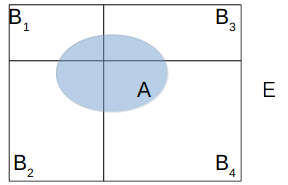
\includegraphics[width=0.51\columnwidth]{A.imagenes/ACV-BioSan-Estat-Bayes.png}
        \caption[Representación geométrica del teorema de Bayes]{Representación geométrica del teorema de Bayes.}
    \end{figure}
\end{multicols}
\section{Combinatoria}
La Combinatoria es la parte de las matemáticas que estudia las técnicas de recuento, en particular, las distintas formas de seleccionar subconjuntos de elementos de un conjunto según unos criterios.
\subsection{Números combinatorios}
El número combinatorio ${n \choose k}$ se define como el número de subconjuntos de $n$ tomados de $k$ en $k$, sin importar el orden y sin repetición. Se calcula como:
\begin{center}
    \begin{equation}
        {n \choose k} = \dfrac{n!}{k!\cdot \left( n - k\right)! }
    \end{equation}
    \captionof{Ecuacion}[Números combinatorios]{Números Combinatorios: Se distinguen cuatro casos especiales:\protect\\
        ${n \choose n} = 1; {n \choose 0} = 1; {n \choose 1} = n; {n \choose n-1} = n$.}
\end{center}
\subsection{Variaciones}
\subsubsection{Variaciones sin repetición}
Se obtiene el número de grupos distintos que se pueden formar con $n$ elementos de forma que cada grupo esté formado por $p$ elementos distintos y que dos grupos son distintos si algún elemento difiere en el orden o en el elemento en sí.
\begin{center}
    \begin{equation}
       V_{n,p} = n - \left( p + 1\right) 
    \end{equation}
    \captionof{Ecuacion}[Variaciones sin repetición]{Variaciones sin repetición.}
\end{center}
\subsubsection{Variaciones con repetición}
Se obtiene el número de grupos distintos que se pueden formar con $n$ elementos de forma que cada grupo esté formado por $p$ elementos repetidos o no y que dos grupos son distintos si algún elemento difiere en el orden o en el elemento en sí.
\begin{center}
    \begin{equation}
        VR_{n,p} = n^p
    \end{equation}
    \captionof{Ecuacion}[Variaciones con repetición]{Variaciones con repetición.}
\end{center}
\subsection{Permutaciones}
\subsubsection{Permutaciones sin repetición}
Se definen diferentes grupos de $n$ elementos distintos que se pueden formar si la diferencia radica en el orden de los mismos.
\begin{center}
    \begin{equation}
        P_n = n!
    \end{equation}
    \captionof{Ecuacion}[Permutaciones sin repetición]{Permutaciones sin repetición.}
\end{center}
\subsubsection{Permutaciones con repetición}
Se definen diferentes permutaciones de $n$ elementos en los que los diferntes elementos se repiten $a, b, \dots k$ veces, respectivamente
\begin{center}
    \begin{equation}
        P_n = \dfrac{n!}{a!\cdot b! \dots k!} \iff a + b +\dots + k = n
    \end{equation}
    \captionof{Ecuacion}[Permutaciones con repetición]{Permutaciones con repetición.}
\end{center}
\section{Variables aleatorias}
Una variable aleatoria ($X$) es una función o fórmula que le asigna a cada elemento $p$ del espacio muestral $\Omega$, un número real ($\R$), llamado ($X_p$). Son siempre cuantitativas, definiéndose como modelo teórico. La función de una variable aleatoria definen sucesos probabilisticos (subconjunto de elementos del espacio muestral) cuando se les asigna un valor, luego la imagen de $X_p$ es la probabilidad de $p$ en la variable $X$. Existen dos tipos:
\begin{itemize}[itemsep=0pt,parsep=0pt,topsep=0pt,partopsep=0pt]
    \item \textbf{Variable aleatoria discreta}: aquella que toma un número finito de valores.
    \begin{figure}[H]
        \centering
        \begin{equation*}
            \begin{split}
                f: \N &\longrightarrow \left[ 0, 1\right] \\
                x_i &\longrightarrow f\left( x_i\right) = P _{\left[ X = x_i\right]} = P _{\left[ e, t.q. X_{\left( e\right)}=x_i \right]}\\
            \end{split}
        \end{equation*}
    \end{figure}
    \item\textbf{Variable aleatoria continua}: aquella que puede tomar un infinito no numerable de valores.
    \begin{figure}[H]
        \centering
        \begin{equation*}
            \begin{split}
                f: \R &\longrightarrow \left[ 0, 1\right] \\
                x_i &\longrightarrow F\left( x\right) = P _{\left[ X \leq x \right]} = \int_{-\infty}^{\infty} f\left( t\right) \cdot dt
            \end{split}                
        \end{equation*}
        \caption*{Variable aleatoria discreta}
    \end{figure}
\end{itemize}
\subsection{Distribución Bernuilli y Binomial}
\subsubsection{Distribución de Bernuilli}
Sea una variable continua $X$, consiste en la realización de un experimento aleatorio con dos posibilidades, éxito o fracaso. La probabilidad de éxito es $p$ y la de fracaso es $q$, que se obtiene de $1-p$. 
\begin{table}[H]
    \begin{tabular}{cc}
        \rowcolor{black}\textcolor{white}{\textbf{Valor}}&\textcolor{white}{\textbf{Probabilidad}}\\
        1&$p$\\
        \rowcolor{hiperlightgray}0&$q = 1-p$\\
        \hline
    \end{tabular}
    \caption[Ejemplo de distribución de Bernuilli]{Ejemplo de distribución de Bernuilli $\left( X\rightarrow \mbox{Ber}_{\left( p\right)} \right)$. En este caso, 1 es \textit{Éxito} y 0 es \textit{Fracaso}. Un ejemplo es el lanzamiento de monedas, siendo 1 sacar cara y 0 no sacar cara.}
\end{table}
\subsubsection{Distribución binomial}
Sea una variable continua $X$ que es una suma de distribuciones de Bernuilli, es decir, consiste en la realización de experimentos aleatorios con varias posibilidade4s, cada una con su probabilidad correspondiente.
\begin{multicols}{2}
    \begin{table}[H]
        \begin{tabular}{cc}
            \cellcolor[HTML]{000000}{\color[HTML]{FFFFFF} Valor} & \cellcolor[HTML]{000000}{\color[HTML]{FFFFFF} Probabilidad}  \\
            $X_1$ & $P_{x_1}$   \\
            \rowcolor{hiperlightgray}$X_2$ & $P_{x_2}$   \\
            $X_3$ & $P_{x_3}$   \\
            \rowcolor{hiperlightgray}$\dots$ & $\dots$  \\
            $X_k$ & $P_{x_k}$ \\
            \hline
        \end{tabular}
        \caption[Ejemplo de distribución binomial]{Ejemplo de distribución binomial.}
    \end{table}
    \columnbreak
    \begin{center}
        \begin{equation}
            P_{\left( X\right) } = {n \choose k}\cdot P^k\cdot Q^{\left(  n-k\right) }
        \end{equation}
        \captionof{Ecuacion}[Formula de una ecuación binomial]{Formula de una ecuación binomial. De la fórmula de la izquierda se puede extraer: $P_{\left( X \right) }$: probabilidad de X; $n$: número total de elementos; $k$: número total de éxitos; $P$: Probabilidad de sacar el suceso; $Q$: Probabilidad de fracaso.}
    \end{center}
\end{multicols}
\subsection{Modelo teórico: media, varianza y dispersión}
Al ser modelos teóricos, existe la necesidad de contrastar estos datos con los reales, de forma que se verifique o no tal modelo.
\begin{itemize}[itemsep=0pt,parsep=0pt,topsep=0pt,partopsep=0pt]
    \item \textbf{Media teórica}: media más probable de obtener según una variable X.
    \begin{center}
        \begin{equation}
            \mu_X = \dfrac{\sum_{i}^{k}\left( P_{x_i}\cdot x_i\right) }{\sum_{i}^{k}P_{x_i}} \xrightarrow[]{\sum_{i}^{k}P_{x_i} = 1} \mu_X = \sum_{i}^{k} \left( P_{x_i}\cdot x_i\right) 
        \end{equation}
        \captionof{Ecuacion}[Formula de la media teórica]{Formula de la media teórica.}
    \end{center}
    \item \textbf{Varianza teórica}: varianza más probable de obtener según una variable X y su media teórica ($\mu_X$).
    \begin{center}
        \begin{equation}
            \sigma_X = \dfrac{\sum_{i}^{k}\left( P_{x_i}\cdot \left( x_i - \mu_X\right)^2\right)  }{\sum_{i}^{k}P_{x_i}} \xrightarrow[]{\sum_{i}^{k}P_{x_i} = 1} \sigma_X = \sum_{i}^{k} \left( P_{x_i}\cdot \left( x_i - \mu_X\right)^2\right) 
        \end{equation}
        \captionof{Ecuacion}[Formula de la varianza teórica]{Formula de la varianza teórica.}
    \end{center}
    \item\textbf{Coeficiente de variación teórico}: raíz cuadrada de la varianza teórica.
    \begin{center}
        \begin{equation}
            CV = \sqrt{\sigma_X} = \sqrt{\sum_{i}^{k} \left( P_{x_i}\cdot \left( x_i - \mu_X\right)^2\right) }
        \end{equation}
        \captionof{Ecuacion}[Formula del coeficiente de variación teórico]{Formula del coeficiente de variación teórico.}
    \end{center}
\end{itemize}
\begin{table}[H]
    \begin{tabular}{ccc}
        \rowcolor{black}&\textcolor{white}{\textbf{Variables de Bernuilli}}&\textcolor{white}{\textbf{Variables continuas}}\\
        Media teórica&$\mu_{\mbox{Ber}} = p$&$\mu_X = \int_{-\infty}^{\infty}x\cdot f\left( x\right) d\left( x\right) $\\
        \rowcolor{hiperlightgray}Varianza teórica&$\sigma_{\mbox{Ber}}^2 = p\cdot q$&$\sigma_X^2 = \int_{-\infty}^{\infty}\left( x -\mu_X\right) \cdot f\left( x\right) d\left( x\right) $\\
        Desviación teórica&$\sigma_{\mbox{Ber}} = \sqrt{p\cdot q}$&$\sigma_X =\sqrt{\int_{-\infty}^{\infty}\left( x -\mu_X\right) \cdot f\left( x\right) d\left( x\right)}$\\
        \hline
    \end{tabular}
    \caption[Definiciones teóricas de valores de centralización]{Definiciones teóricas de valores de centralización. Las variables de Bernuilli, al ser únicamente dos casos los posibles, las definiciones son sencillas; mientras que las variables continuas se definen mediante integrales.}
\end{table}
\subsection{Operaciones con variables aleatorias}
Toda variable aleatoria es en esencia una función cuya imagen asigna una probabilidad a un valor $x_i$. Al ser una función, también se le pueden sumar, restar, multiplicar y dividir números para obtener resultados proporcionales o hacer combinaciones lineales con otras funciones y obtener otra cualquiera.
\begin{equation*}
    X_{a,b}\xrightarrow{\exists}\left\lbrace \begin{array}{c}
        A\cdot X_{a,b}\\
        X_{a,b} + A\\
        X_{a,b}^A\\
        X_{1\left( a,b\right) } + X_{2\left( a,b\right) }\\
    \end{array}\right\rbrace 
\end{equation*}
Fuere cual fuere la operación practicada, la media, varianza y desviación típica de la función operada guardar una relación con la función no operada.
\begin{table}[H]
    \begin{tabular}{cccc}
        \rowcolor{black}&\textcolor{white}{$a,b$ números cualesquiera}&\textcolor{white}{$X_1,X_2$ variables dependientes}&\textcolor{white}{$X_1,X_2$ variables independientes}\\
        Media &$\mu_{a\cdot x+b} = a\cdot \mu_X + b$&$\mu_{X_1 + X_2} = \mu_{X_1} + \mu_{X_2}$&$\mu_{X_1 + X_2} = \mu_{X_1} + \mu_{X_2}$\\
        \rowcolor{hiperlightgray}Varianza &$\sigma_{a\cdot X + b} = a^2\cdot\sigma_X^2$&&$\sigma_{X_1 + X_2}^2 = \sigma_{X_1}^2 + \sigma_{X_2}^2$\\
        \hline
    \end{tabular}
    \caption[Operaciones con valores de centralización]{Operaciones con valores de centralización.}
\end{table}
    \part{Bioquímica}
    \chapter{Introducción}
\chapter{Proteínas}
\section{Aminoácidos}
\subsection{Introducción: clasificación y propiedades}
    
    \part{Botánica y Fisiología vegetal}
    \part{Citología e Histología}
     \chapter{Introducción y teoría celular}
\section{Teoría celular}
La teoría celular fue elaborada por tres grandes científicos como J.M Schleiden (enunciándola en 1938), T. Schwann (1939) y R. Virchow (1955) que establece tres elementos fundamentales:
\begin{itemize}[itemsep=0pt,parsep=0pt,topsep=0pt,partopsep=0pt]
    \item La célula es la unidad funcional y estructural de los seres vivos.
    \item Todos los seres vivos está compuestos por una o más células.
    \item Toda célula proviene de otra célula\footnote{\textit{omnis cellula ex cellula}, enunciado de Virchow.}.
\end{itemize}
\section{Organización celular}
Desde el punto de vista de la organización, las células se clasifican en dos grupos, a saber, procariotas y eucariotas, con notables diferencias:
\begin{table}[H]
    \begin{tabular}{N{3.25cm}M{6cm} M{6.9cm}}
        \rowcolor{black}\textcolor{white}{\textbf{}}&\textcolor{white}{\textbf{Procariotas}}&\textcolor{white}{\textbf{Eucariotas}}\\
        Organización celular&Unicelular&Unicelular o pluricelular\\
        \rowcolor{hiperlightgray}Tamaño (aprox)&1 a 10 $\mu$m&10 a 50 $\mu$m\\
        Envoltura nuclear&Ausente&Doble\\
        \rowcolor{hiperlightgray}Compartimentación&No&Sí\\
        Orgánulos&No&Sí (Retículo endoplásmico, Aparato de Golgi, Mitocondrias, Lisosomas, Peroxisomas)\\
        \rowcolor{hiperlightgray}Citoesqueleto&No&Sí\\
        Genoma&Sin histonas, circular, citoplasmático&Con histonas y otras proteínas, Lineal, nuclear\\
        \rowcolor{hiperlightgray}Nucléolo&No&Sí\\
        Ribosomas&70S (50S y 30S)&80S (60S y 40 S)\\
        \hline
    \end{tabular}
    \caption[Diferencias entre procariotas y eucariotas]{Diferencias entre procariotas y eucariotas.}
\end{table}
\subsection{Células eucariotas}
Las células eucariotas se dividen en compartimentos principales:
\begin{itemize}[itemsep=0pt,parsep=0pt,topsep=0pt,partopsep=0pt]
    \item \textbf{Citoplasma}: parte localizada fuera del núcleo. Contiene orgánulos e inclusiones en un gel acuoso concentrado denominado citosol o matriz citoplasmática. La matriz está compuesta por un 70 a 80 \% de agua y solutos desde iones inorgánicos, metabolitos intermedios, glúcidos, lípidos, proteínas y ARN.
    \item \textbf{Núcleo}: el núcleo es un compartimento limitado por una membrana (envoltura nuclear) que contiene al material genético (ADN) junto con la maquinaria necesaria para la replicación y su transcripción y procesamiento a ARN.
    \item\textbf{Protoplama}: constituye todo el interior celular, sumando citoplasma y núcleo.
\end{itemize}
\chapter{Membrana plasmática}
La membrana plasmática es una barrera semipermeable que separa el medio extracelular del intracelular, así como la delimitación entre orgánulos celulares y el citoplasma (llamadas entonces membranas citoplasmáticas). Debido a que actúa como barrera selectiva al paso de las moléculas, la membrana plasmática determina la composición del citoplasma. Dado su pequeño tamaño (8 a 10 nm), no es visible con el microscopio óptico.

En la actualidad, el modelo más aceptado es el propuesto por Singer y Nicolson (1972), llamado \textbf{modelo de mosaico fluido}:
\begin{itemize}[itemsep=0pt,parsep=0pt,topsep=0pt,partopsep=0pt]
    \item La membrana está formada por lípidos, proteínas y glúcidos que se disponen en una configuración estable de baja energía.
    \item Los lípidos se orientan formando una doble capa lipídica en la que se disponen proteínas que interaccionan entre sí y con los lípidos, con capacidad limitada de movimiento lateral.
    \item Las membranas biológicas son estructuras asimétricas en cuanto a la distribución de sus componentes, ya que los glúcidos se localizan exclusivamente en la cara externa de la membrana plasmática.
\end{itemize}
\section{Composición química}
En la mayoría de los tipos celulares, la membrana plasmática se compone de un 50 \% de lípidos y otro tanto de proteínas en peso. Como las proteínas son mucho más grandes, este porcentaje corresponde más o menos a una molécula de proteína por cada 50 a 100 de lípidos. Algunas membranas varían estos porcentajes, como la mitocondrial (75 \% de proteínas) o la vaina de mielina (sólo 20\% de proteínas).
\subsection{Lípidos de membrana}
Los lípidos tienen carácter anfipático y cuando se encuentran en un medio acuoso se orientan formando una bicapa, enfrentando los grupos hidrófilos al medio acuoso y los hidrófobos en el centro. Entre estos, se encuentran tres grupos de familias químicas:
\subsubsection{Fosfolípidos}
Contienen un residuo de ácido fosfórico mediante enlace éster. Se dividen en:
\begin{itemize}[itemsep=0pt,parsep=0pt,topsep=0pt,partopsep=0pt]
    \item \textbf{Fosfoglicéridos}: son los lípidos más abundantes, compuestos por glicerol esterificado en sus posiciones 1 y 2 (diacilglicerol) con ácidos grasos y un grupo fosfato (posición 3). Los principales son la fosfatidilcolina (lecitina), fosfatidilserina, fosfatidiletanolamina (cefalina), fosfatidilinositol, fosfatidilglicerol y difosfatidilglicerol (cardiolipina). La fosfatidilcolina es el fosfoglicérido principal de las membranas plasmática y citoplasmáticas; y la cardiolipina el de las mitocondriales.
    \item\textbf{Esfingolípidos}: compuestos derivados de la esfingosina (o ceramida, 2-amino-4-octadecen-1,3-diol) . La esfingosina unida a fosfocolina o fosfoetanolamina forman las esfingomielinas, abundantes en la vaina de mielina.
\end{itemize}
\subsubsection{Glucolípidos}
La ceramida unida a glúcidos forma los glucoesfingolípidos, que se localizan en la cara externa de la membrana plasmática. Pueden ser:
\begin{itemize}[itemsep=0pt,parsep=0pt,topsep=0pt,partopsep=0pt]
    \item \textbf{Cerebrósidos}: la ceramida se una a un monosacárido, ya sea galactosa (galactocerebrósidos), en las membranas del tejido nervioso; o a glucosa (glucocerebrósidos), en tejidos no nerviosos.
    \item\textbf{Gangliósidos}: la ceramida se une con oligosacáridos con al menos un residuo de ácido siálico (N-acetilneuramínico), con carga negativa. Abundantes en células nerviosas.
\end{itemize}
\subsubsection{Colesterol}
El colesterol es un lípidos de unos 27 carbonos que representa el 40 \% de los lípidos de membrana, encargado de regular la fluidez de ésta.
\subsubsection{Movimientos de los lípidos}
Los componentes de la membrana tienen una posibilidad de movimiento limitada que le permite cierta fluidez a ésta. Pueden ser:
\begin{itemize}[itemsep=0pt,parsep=0pt,topsep=0pt,partopsep=0pt]
    \item \textbf{Difusión lateral}: las moléculas se desplazan en 2 dimensiones siguiendo el plano de la membrana.
    \item\textbf{Rotación}: la molécula puede girar sobre su eje mayor.
    \item\textbf{Flexión}: las cadenas de ácidos grasos pueden flexionarse o doblarse dentro de la doble capa.
    \item\textbf{Flip-Flop}: movimiento en el que una molécula se transloca (normalmente por acción de una enzima translocasa) de una monocapa a otra.
\end{itemize}
\subsubsection{Lípidos y fluidez}
La fluidez de las membranas depende de los lípidos y es una característica fundamental para la transducción de señales. Depende a su vez de factores como la temperatura, concentración de colesterol y naturaleza de los fosfolípidos y de la longitud y grado de insaturaciones de los ácidos grasos.

La fluidez de incrementa con la temperatura, la presencia de lípidos insaturados y de cadena corta y la falta de colesterol. El colesterol se inserta en la bicapa con sus grupos apolares próximos a la cabeza de los fosfolípidos, interfiriendo con el movimiento de las cadenas de ácidos grasos, así como impedir un gran empaquetamiento en las cadenas de estos en caso de bajas temperaturas.
\subsubsection{Distribución asimétrica}
Existe una mayor proporción de fosfatidilcolina y esfingomielina y esterificaciones de ácidos grasos saturados en la hemimembrana E o exoplasmática, y mayor cantidad de fosfatidilcolina y fosfatidilserina (es marcador de apoptosis y señal para macrófagos para que la fagociten) y esterificaciones ácidos grasos insaturados, en la hemimembrana P o citoplasmática. Debido a su mayor contenido en ácidos grasos insaturados, la hemimembrana P es más fluida.

En la membrana pueden encontrarse regiones de lípidos implicadas en la señalización celular, denominándose microdominios o balsas lipídicas (\textit{rafts}), teniendo mayor riqueza en esfingolípidos y colesterol. Los esfingolípidos poseen largas cadenas de ácidos grasos saturados, lo que hace que las balsas lipídicas sean más espesas y menos fluidas que el resto de la membrana. Las caveolas están estrechamente relacionadas con estos \textit{rafts} y son invaginaciones de membrana recubiertas de la proteína caveolina, mediadora en la endocitosis.
\subsection{Proteínas de membrana}
Las proteínas son características de cada tipo celular y confieren a la membrana sus funciones biológicas. Su distribución es asimétrica y según su disposición en la membrana se habla de proteínas integrales (intrínsecas) o periféricas (extrínsecas).
\subsubsection{Proteínas integrales}
Las proteínas integrales están firmemente unidas a lípidos por interacciones hidrofóbicas, por lo que sólo se disocian de éstos mediante tratamientos drásticos que destruyen la integridad de la membrana como detergentes. Una de sus funciones principales es la recepción de ligandos.

Las proteínas integrales suelen atravesar la membrana por completo, siendo proteínas transmembrana. Si sobresalen por ambos lados de la doble membrana, se denominan monopaso, bitópicas o de paso único. Si emerge varias veces, se habla de proteínas multipaso, politópicas o de paso múltiple. Las proteínas que se anclan a la membrana pero no la atraviesan se denominan monotópicas. Su orientación con respecto a las hemimembranas  se determina en el retículo endoplásmico.
\subsubsection{Proteínas periféricas}
Las proteínas periféricas sobresalen solo por uno de los lados de la membrana celular y no se asocian a lípidos, por lo que pueden extraerse sin necesidad de alterar la bicapa. Este tipo de proteínas se pueden unir a una proteína integral, a un lípido o a un oligosacárido unido a un lípido.

Al igual que los lípidos, tienen movimiento de rotación y difusión, pero no de translocación.
\subsection{Glúcidos de membrana}
Están representados en su mayoría por oligosacáridos unidos covalentemente a segmentos o dominios de proteínas o lípidos, formando, en cada caso, glucoproteínas o glucolípidos. Su distribución es exclusiva de la hemimembrana E, constituyendo la cubierta celular o glucocálix, en la que pueden encontrarse algunas proteínas.

Los oligosacáridos unidos a proteínas pueden unirse a asparagina (N-oligosacáridos) o a treonina o serina (O-oligosacáridos). Los que están unidos a lípidos se unen fundamentalmente a esfingolípidos y en menor medida al fosfatidilinositol.

Las principales funciones son:
\begin{itemize}[itemsep=0pt,parsep=0pt,topsep=0pt,partopsep=0pt]
    \item Presentan propiedades inmunológicas, ya que los glúcidos conforman el sistema ABO y MN.
    \item Interviene en los fenómenos de reconocimiento celular, importantes durante el desarrollo embrionario.
    \item Contribuye al reconocimiento y fijación de sustancias a incorporar mediante pinocitosis o fagocitosis.
    \item Participa en las uniones celulares entre sí y con la matriz extracelular.
    \item Es responsable (por el ácido siálico) de la carga negativa de la superficie celular.
\end{itemize}
\subsection{Renovación de la membrana}
La membrana plasmática se encuentra en un continuo proceso de reciclaje debido a procesos de endocitosis y exocitosis. La renovación se realiza a partir de membranas del aparato de Golgi, procedentes a su vez del retículo endoplásmico, lugar donde se sintetizan las membranas citosólicas y plasmáticas pero no de mitocondria ni cloroplasto. 
\subsection{Membrana eritrocitaria}
Las proteínas de membrana más estudiadas con las del eritrocito dada la facilidad para obtenerlas. Se compone, además de la cantidad antes descrita de lípidos y glúcidos, de:
\begin{itemize}[itemsep=0pt,parsep=0pt,topsep=0pt,partopsep=0pt]
    \item \textbf{Glucoforina}: glucoproteína transmembrana cuyo segmento externo se une a oligosacáridos, principalmente ácido siálico.
    \item\textbf{Proteína de la banda 3}: proteína transmembrana de paso múltiple que posee alrededor de 14 segmentos transmembrana que forman un canal para el transporte antiparalelo de \ch{Cl^-} y \ch{HCO^{3-}}.
    \item\textbf{Espectrina}: principal proteína periférica de la membrana del eritrocito, es un tetrámero constituido por dos cadanas $\alpha$ y dos cadena $\beta$ que se asocian con filamentos de actina para formar una red bajo la membrana plasmática.
    \item\textbf{Anquirina}: forma un nexo de unión entre el dominio citoplásmico de la proteína de la banda 3, la actina y la espectrina.
    \item\textbf{Proteína 4.1}: fija y une el dominio citoplásmico de la glucoforina junto con la red de actina y espectrina.
\end{itemize}








     \chapter{Transporte a través de membranas}
\section{Transporte de moléculas pequeñas}
El transporte de moléculas pequeñas a través de membrana no modifica su morfología y se lleva a cabo sin la participación del citoesqueleto. Puede ocurrir mediante los siguientes mecanismos.
\begin{table}[H]
    \begin{tabular}{M{3.5cm}M{4cm}N{3.5cm} N{4cm}}
        \multirow{6}{3.5cm}{Dependencia de energía} & \multirow{3}{4cm}{\textbf{Transporte pasivo}\\
             (a favor de gradiente, sin consumo de energía)} & \multicolumn{2}{N{7cm}}{Difusión pasiva o  simple} \\
        &  & \multirow{2}{3.5cm}{Difusión facilitada} & Proteínas transportadoras \\
        &  &  & Proteínas canal \\
        & \multirow{3}{4cm}{\textbf{Transporte activo}\\(en contra de gradiente, consumo de energía)} & \multirow{2}{4cm}{Primario (hidrolisis de ATP)} & ATPasa de \ch{Na^+}/\ch{K^+}; ATPasa de \ch{Ca^{2+}} \\
        &  &  & Transportadores ABC \\
        &  & \multicolumn{2}{N{7cm}}{Secundario (energía en gradiente iónico)} \\
        \hline
        \multirow{2}{3.5cm}{Dirección de los compuestos transportados} & \multirow{2}{4cm}{Uniporte o transporte simple} & \multicolumn{2}{N{7cm}}{Cotransporte} \\
        &  & Paralelo o simporte & Antiparalelo o antiporte
    \end{tabular}
    \caption[Modalidades de transporte a través de membrana\label{tab:CITO:Transporte:ModalidadTransporte}]{Modalidades de transporte a través de membrana.}
\end{table}
\subsection{Transporte pasivo}
El transporte pasivo de moléculas se efectúa a favor de gradiente de concentración o carga eléctrica, por lo que no se produce gasto de energía. Se puede diferenciar entre una forma simple o facilitada.
\subsubsection{Difusión pasiva o simple}
El mecanismo más sencillo mediante el que las moléculas pueden atravesar la membrana plasmática es la difusión pasiva: una molécula se disuelve en la bicapa lipídica, difunde a través de ella y después se disuelve en la solución acuosa al otro lado de la membrana. Gracias a este mecanismo, las sustancias atraviesan esta membrana desde la zona más concentrada a la más diluida hasta igualar concentraciones a ambos lados.

La membrana plasmática deja pasar con facilidad pequeñas moléculas no polares (\ch{O_2}, \ch{N_2}, benceno), y moléculas pequeñas polares sin carga (agua, urea, glicerol, \ch{CO_2}). El agua se mueve con más facilidad y se desplaza hacia donde los solutos están más concentrados mediante un proceso de ósmosis.
\subsubsection{Difusión facilitada}
Las moléculas se desplazan a favor de gradiente de concentración y, en el caso de moléculas cargadas, de potencial eléctrico. La difusión facilitada se diferencia en que las moléculas no se disuelven en la bicapa lipídica y necesitan la participación de una proteína transportadora para atravesarla. Existen dos clases de proteínas, las transportadoras y las que forman canales.
\begin{itemize}[itemsep=0pt,parsep=0pt,topsep=0pt,partopsep=0pt]
    \item \textbf{Proteínas transportadoras}: Las proteínas transportadoras (carriers o permeasas) son proteínas integrales de membrana que sufren un cambio conformacional durante el transporte. Muy selectivas, a menudo sólo transportan un tipo de molécula. Permiten el paso de determinadas moléculas o iones, saturándose el transporte a determniadas concentraciones. La cinética del transporte es similar a la de las reacciones enzimáticas. Son responsables de la difusión de glúcidos, nucleótidos y aminoácidos.
    \item\textbf{Proteínas canal}:
\end{itemize}

    \part{Embriología}
    \part{Fisiología}
    \part{Genética y Biología Molecular}
    \part{Microbiología}
    % SEC I - Introducción
     \clearpage
\chapter{Introducción}
\label{chapter:Introduccion}
\section{Introducción}
\label{chap1:sec:introduccion}
La Microbiología es la ciencia que estudia a los microorganismos en relación a su estructura, fisiología, genética, taxonomía y aplicaciones. Estudia a los microorganismo de forma holística y en cada una de sus estructuras.

Un microorganismo es un ente biológico acelular, unicelular, pluricelular o cenocítico sin organización tisular y que requiere una metodología especial de estudio (cultivo puro)
\section{Cronología y <<Teoría de la Generación espontánea>>}
\label{chap1:sec:cronologia}
Algunos hechos notables en la historia de esta disciplina son:
\begin{itemize}[itemsep=0pt,parsep=0pt,topsep=0pt,partopsep=0pt]
	\item \textbf{Hoocke}: descubrimiento de los cuerpos fructíferos de hongos
	\item \textbf{A. van Leeuwenhoek}: descubrimiento de ciertas bacterias o “animálculos”
	\item \textbf{R. Koch}: Observación del Bacillus anthracis
	\item Microscopios y lentes de Abbe y Zeiss
	\item \textbf{Ziehl} y \textbf{Neelsen}: descripción del Mycobacterium tuberculosis
	\item \textbf{C. Gram}: tinción selectiva para microorganismos
	\item \textbf{Loeffter}: Tinción de flagelos.
\end{itemize}

\paragraph{Generación espontánea}: hasta mediados del siglo XIX, la única teoría aceptada para el origen de la vida era por generación espontánea. Los experimentos de Francesco Redi en el siglo XVII la invalidaron para seres pluricelulares. El descubrimiento del $0_2$ y de la química de los gases, junto con las controversias entre Needham y Spallanzani mantuvieron vivo el debate hasta la llegada de Pasteur, quien aboliría la teoría para el mundo microbiano.  

Los experimentos de Pasteur consistían en calentar para desinfectar un caldo de carne en un matraz. Curvó el cuello del matraz en forma de ese itálica para aislarlo del exterior, pero que siguiese entrando O2. Al no observar contaminación, probó a romper la boca del matraz, dejando expuesto el caldo de cultivo, que esta vez sí se infectó. Así, por tanto, dedujo Pasteur que la contaminación solo podía venir de microorganismo que estaban en el aire, y no se generaban espontáneamente.

Tyndall descubrió que el calor no siempre mataba a los microorganismos, no a todos. Así, observó que en cultivos a base de infusiones de heno, no todos los microorganismos eran termolábiles, algunos resistían las altas temperaturas y lo contaminaban. Fue el investigador Ferdinand Cohn quien descubrió que los microorganismos termorresistentes forma una estructura, la endospora, que sobrevivía a su forma vegetativa. Esta estructura de resistencia es muy común del género \textit{Bacillus}.
\section{Microorganismos y Ciclos biogeoquímicos. Transformación de materia. Patogenia}
\label{chap1:sec:totumrevolutum}
Los microorganismos juegan papeles bastante reseñables en la transformación de materia y patogenia. Uno de los primeros investigadores en estos campos fue Pasteur, quien describió las fermentaciones alcohólica, láctica y butírica, así como el aislamiento del primer ser anaerobio estricto, \textit{Clostridium}.

Para el estudio de microorganismo es necesaria una metodología especial, que es el cultivo puro, es decir, su aislamiento en ciertos medios para su estudio. La primera técnica fue creada por Joseph Lister (1878) por diluciones. Le siguió Emil Hansen (1886) con las diluciones seriadas. Robert Koch propuso el método de cultivo en medio sólido. En una base de agar-agar, inerte y no comestible, al añadírsele a un líquido, este se solidificaba. Creador del asa de siembra, descubrió que todos los organismos provenientes de una masa aislada en cultivo procedían del mismo individuo, que había formado una colonia.

Los primeros investigadores en relacionar a los microorganismos con los ciclos biogeoquímicos fueron Beijerinck y Winogradsky. Beijerinck, que ideó además el cultivo por enriquecimiento, descubrió que intervenían en el ciclo del nitrógeno al fijar nitrógeno molecular en el suelo, siendo los géneros \textit{Rhizobium} (en simbiosis) y \textit{Azotobacter}. Winogradsky fue el primero en observar la autotrofía en bacterias quimiolitotrofas (obtenían el carbono del $CO_2$ ambiental y la energía de reacciones químicas inorgánicas).

La idea de que algunos microorganismos podían originar enfermedades nació a partir de 1850, cuando Ignaz Semmelweis propuso que estos seres podían ser la causa de la fiebre puerperal. En 1860, Lister, en busca de prevenir estas enfermedades, lanzó la idea de la cirugía aséptica, con escaso éxito. Pero el científico que más trabajo en el campo de los microorganismos patógenos, fue Robert Koch. Asiló a los agentes del carbunco (\textit{Bacillus anthracis}) y de la tuberculosis (\textit{Mycobacterium tuberculosis}, o bacilo de Koch). Así mismo, desarrolló los postulados de Koch que permiten establecer si una enfermedad es causada o no por un microorganismo. Son:
\begin{enumerate}[itemsep=0pt,parsep=0pt,topsep=0pt,partopsep=0pt]
	\item El agente patógeno se halla en individuos enfermos, pero no en sanos
	\item Es posible aislar en medio de cultivo el patógeno en sangre del individuo enfermo
	\item Si se le inocula a un individuo aislado el microorganismo aislado, enferma.
	\item Es posible volver a aislar el patógeno en la sangre de un individuo inoculado, que es igual al del primer individuo.
\end{enumerate}
\begin{figure}[htbp]
	\centering
	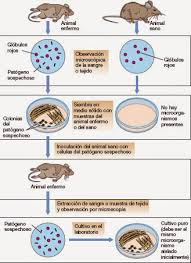
\includegraphics[trim={0 2cm 0 0},clip,width=0.8\columnwidth]{./A.imagenes/ACV-MICROBIO-PostuladosKoch}
	\caption[Postulados de Koch]{Representación de los postulados de Koch. \textit{\textbf{Extraido de}}: \protect\cite{Brock2012}}
\end{figure}

Además de las bacterias y otros microorganismos patógenos, existen otros agentes causantes de enfermedades, capaces de atravesar filtros microscópicos que las bacterias eran incapaces por su tamaño, los virus. El primero en ser descubierto fue el virus del mosaico del tabaco por Beijerinck e Ivanovsky. Así les siguieron el de la glosopeda (Loffler y Frosch), los bacteriófagos (Twort y D'Herelle). Importantes fue también la hipótesis sobre la replicación del virus del sarcoma de Rous (Temin), o el descubrimiento del VIH (Montaigner, Gallo).

En el desarrollo de la quimioterapia, una idea fundamental fue el concepto de <<bala mágica>> de Paul Erlich, que desarrolló el Salvarsán (compuesto 606) frente a la sífilis. Domayeck descubrió que el colorante Prontosil rubrum era efectivo contra estafilococos y estreptococos. Pero no fue hasta 1929 en él se creó el concepto de antibiótico con el descubrimiento de la penicilina por A. Fleming a partir de Penicilium notatum. Fueron Florey y Chain quienes consiguieron aislar en cultivos y producirla a gran escala. Para 1940, Selmen Walkman descubrió la actinomicina, la estreptomicina y la neomicina.

Un hito importante en la relación entre microorganismos y patogenia fue la creación de las vacunas  por Edward Jenner a finales del siglo XVIII. Al observar que las vaqueras en contacto con vacas con la variante bovina de la viruela eran inmunes a la cepa humana, descubrió que inoculando las costras del ganado en humanos, estos se inmunizaban. Pasteur, que utilizaba microorganismos sin poder patogénico pero sí inmunológico, creó vacunas atenuadas para la rabia o al cólera aviar. Salmon y Smith descubrieron que los microorganismos muertos por procesos físicos o químicos podían provocar inmunidad en caso de ser inoculados. Así se crearon vacunas contra la fiebre tifoidea (Widal), cólera (Haffkine) o tuberculosis, cólera, rabia y tifus (Clúa)

En el campo de la genética, algunos microorganismos o microbiólogos han tenido relación con grandes avances en esta rama. Así, el Dogma Central de la Biología Molecular de  <<1 gen: 1 enzima>> fue comprobado mediante experimentos con el moho rojo del pan, diseñados por Beadle y Tatum. La técnica de la PCR desarrollada por Kary Mullis para la clonación de genes usó enzimas de microorganismos que intervenían en la replicación del DNA.
\section{Aplicaciones de la Microbiología}
\label{chap1:sec:aplicaciones}
Los microorganismos son los seres vivos mejor conocidos dado su simplicidad estructural. Ello, junto con la facilidad de manipulación genética y su elevada tasa de crecimiento, permite usarlos para ciertos procesos con interés para los humanos en diferentes áreas, por transformación química de sustratos. Así, en la industria alimentaria pueden ser utilizados para la mejora de producción de un determinado producto, obtención de algún compuesto o en controles de calidad. En la agricultura y la ganadería, como insecticidas biológicos, cepas fijadoras de nitrógeno (abonado) o como suplemento alimentario para ganado. En el cuidado del medio natural, pueden servir para la biorremediación de suelos, reciclado de basuras y depuración de aguas, destoxificación de efluentes,… En la lucha frente a patógenos, puede ser útil la microbiología en síntesis de nuevos fármacos, tecnología de vacunas o nuevos métodos de diagnóstico.
\section{Diversidad del mundo microbiano}
\subsection{Microorganismos con estructura celular}
Los microorganismos con estructura celular, es decir, vivos, se pueden clasificar en dos grandes grupos, según presenten o no su material genético encerrado en una membrana (núcleo): procariotas (sin núcleo) y \textit{Eukarya} (con núcleo). Las procariotas a su vez se dividen en \textit{Archaea} y \textit{Bacteria}.
\subsubsection{Dominio \textit{Bacteria}}
Procariota (no presenta membrana nuclear, el material genético se presenta en el citoplasma, en una región denominada nucleoide). El material genético lo constituye, de forma general, un único cromosoma (algunos presentan mayor número) de forma circular (también se han advertido en forma lineal). Presenta también moléculas de DNA dúplex circular, con información no fundamental para el desarrollo pero que si le otorga ventajas frente a otros entes. Codifican enzimas de resistencia a antibióticos, toxinas, utilización de otros sustratos (Plásmido Tol (tolueno)).

Mayoritariamente son unicelulares, aunque a veces formen colonias o estructuras cenocíticas. La mayoría presentan pared celular, siendo de peptidoglucano (mureína). La membrana celular es muy similar a las del género \textit{Eukarya}, es decir, una estructura de bicapa lipídica enfrentando porciones hidrófobas.  En su citoplasma se hallan ribosomas de 70S y se advierta la inexistencia de orgánulos membranosos (de membrana unitaria), a excepción de los tilacoides de cianobacterias. Algunas de las funciones de los orgánulos membranosos de los eucariontes lo llevan a cabo otras estructuras, como por ejemplo la pared bacteriana, que puede realizar la función de obtención de energía de las mitocondrias. Presentan estructuras exclusivas de este dominio como son los pili o las fimbrias.

En cuanto a su morfología se pueden clasificar en cocos (esféricas), bacilos (forma de barra), espirales (forma espiral), vibrios (forma de coma). Según su motilidad, pueden ser sésiles (sin capacidad de moverse), o móviles (con capacidad de moverse, poseen una estructura particular que es el flagelo, distinto de los eucariontes). No existen procesos de reproducción sexual, se reproducen por fisión binaria. No obstante, se observan procesos de parasexualidad (intercambio de material genético): transformación, transducción y conjugación.
\subsubsection{Dominio \textit{Archaea}}
Son seres procariotas (no presenta membrana nuclear, el material genético se presenta en el citoplasma, en una región denominada nucleoide). El material genético lo constituye, de forma general, un único cromosoma de forma circular 

Este clado posee, en gran parte de sus individuos, la característica de tener pared celular, constituida en muchos casos de pseudopeptidoglucano (pseudomureína). La membrana plasmática no está formada por esteres de glicerol, sino por glicerol unido a cadenas de isoprenos (metil-1,3-butadieno) por enlaces éter. Esta característica les permite habitar lugares con condiciones ambientales límite (extremófilas). Poseen flagelos y cilios, pero de composición diferente al resto de taxones. No existen seres, en esta división taxonómica, que sean patógenos ni fotosintéticos.
\subsubsection{Dominio \textit{Eukarya}}
Este dominio se subdivide en tres grupos:
\begin{itemize}[itemsep=0pt,parsep=0pt,topsep=0pt,partopsep=0pt]
	\item \textbf{Hongos}: quimioorganotrofos heterótrofos, poseen un núcleo verdadero (eucariontes), y se alimentan por absorción. Son seres no fotosintéticos, con una pared celular de quitina y otros glucanos. Pueden reproducirse de forma asexual y sexual. Son patógenos oportunistas, sólo son invasivos en casos de inmunodepresión (\textit{Penicilium}, \textit{Aspergillus}). Se clasifican en 
	\begin{itemize}[itemsep=0pt,parsep=0pt,topsep=0pt,partopsep=0pt]
		\item \textit{\textbf{Filamentosos}}: mohos.
		\item \textit{\textbf{Unicelulares}}: levaduras.
		\item \textit{\textbf{Mucosos}}: forman esporas y son móviles. Menos desarrollados, se alimentan de bacterias.
	\end{itemize}
	\item \textbf{Algas}: eucariontes, pueden ser unicelulares de vida libre o colonial. Son fotosintéticas, con una pared celular de celulosa. Son de hábitats acuáticos.
	\item \textbf{Protozoos}: eucariontes, unicelulares. Se alimentan por ingestión. De hábitat acuático y sin pared celular. Suelen ser comensales o patógenos.
\end{itemize}
\subsection{Entidades acelulares}
\subsubsection{Virus}
Partículas infectivas, parásitos obligados, constan de una cápside proteica que encierra que encierra al material genético, que en el caso de los virus puede ser DNA o RNA, en todas la forma posibles (lineal o circular; doble o monocatenario;$\dots$). Al conjunto de cápside y material genético se le denomina nucleocápside, pudiendo estar o no recubierta de una vesícula de membrana unitaria de su anterior huésped (cubiertos o desnudos, respectivamente). Algunos virus tienen enzimas en la nucleocápside, como la lisozima o las transcriptasas, necesarias para algún proceso de su ciclo vital. Algunos virus son satélites, es decir, que necesitan de otro virus para poder infectar a una célula. Un ejemplo es el virus de la hepatitis D, que precisa infectar junto al de la hepatitis B.
\subsubsection{Viroides}
Partículas de RNA simplexo circular con estructura secundaria (especialmente puentes intracatenarios, simulando una estructura dúplex) infectivos, patógenos de plantas. Con una medida de 250 a 400 nucleótidos, se desconoce qué codifican. Fueron descubiertos por Diener en 1967. 
\subsubsection{Priones}
Moléculas patógenas formadas por proteínas, variantes conformacionales de proteínas propias, con la misma estructura primaria, pero distinta secundaria, la cual pueden transmitir a otra proteína con la conformación no patógena. Producen enfermedades como el Kuru, la encefalopatía espongiforme bovina y humana o el Corea de Huntington.
\subsection{Propuestas de clasificación}
En el momento del descubrimiento de los microorganismos, estos seres se incluyeron en los reinos ya descritos, es decir, en animales o plantas. No será hasta 1866 cuando por parte del biólogo Haeckel los clasifique, a aquellos seres sin núcleo en el reino Monera o Protista, juntando a todos los procariotas. 

En 1930, con el microscopio electrónico, Chalton establece el término procariota tras estudios de estructura celular, concepto que defendió en 1960 Murray. Para 1969, el científico Whitaker, siguiendo criterios de estructura celular, clasificó a los seres vivos en 5 reinos: \textit{Monera} (bacterias), \textit{Protoctista} (protozoos y algas), \textit{Funghi}, \textit{Plantae} y \textit{Animalia}.

En la década de 1970, al albor de la Biología Molecular, con la secuenciación de ácidos nucleicos, se pueden clasificar filogenéticamente a las especies por la similitud de estas macromoléculas. De todo el material genético celular, se estudia el RNA ribosómico (RNAr) de 16S (procariotas) ó 18S (eucariotas). Estos cronómetros moleculares se utilizan frente a otros fragmentos por su ubicuidad, su pronta aparición en la evolución, su pequeño tamaño, frente a otros genes, por la conservación de su función y de parte de la secuencia.

Propuesta por Woesse en 1977, diferenció tres dominios con un ancestro común a todos (LUCA): las bacterias por un lado, y Archaea y eucariontes por otro lado. Así, los procariotas forman un grupo bifilético frente a unas eucariotas monofiléticas.

Dentro de la clasificación de Woesse, se pueden diferenciar los siguientes subclados:
\begin{itemize}[itemsep=0pt,parsep=0pt,topsep=0pt,partopsep=0pt]
	\item \textit{\textbf{Bacteria}}: numerosos filos de los que se puede destacar \textit{Cyanobacteria}, Gram positivas, \textit{Chlamydia} (parásitos intracelulares obligados, algunos provocan ETSs), \textit{Proteobacteria} (dominio de mayoría Gram negativa, están \textit{E. colli} o \textit{Salmonella})
	\item \textit{\textbf{Archaea}}: dos filo principales: \textit{Euryarchaeota} y \textit{Crenarcheaota}. Son procariotas extremófilos.
	\item\textbf{\textit{Eukarya}}: se encuentra el reino Funghi, Plantae y Animalia.
\end{itemize}
\begin{figure}[H]
	\centering
	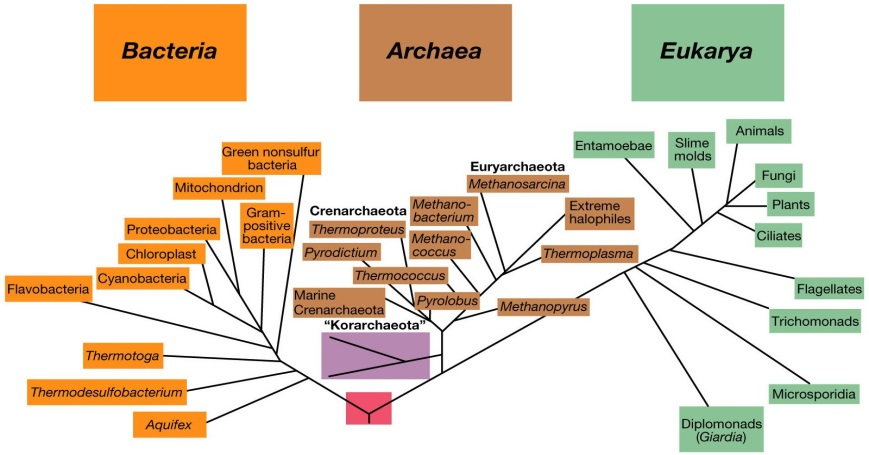
\includegraphics[width=\columnwidth]{A.imagenes/ACV-MICROBIO-PropuestaClasificacion}
	\caption[Propuesta de clasificación de Microorganismos]{Propuesta de clasificación de Microorganismos. Todas descenderían de un mismo replicador que por diversas mutaciones, daría lugar al conjunto de la vida. \textit{\textbf{Extraído de}}: \cite{Prescott2011}}
\end{figure}

     \chapter{Observación microscópica}
Microscopio óptico de campo claro con objetivo de inmersión x100. Los objetivos de 10x y 40x se usan para enfocar los microorganismos. El aumento viene determinado por:
\begin{equation}
	\mbox{Aumento total} = \mbox{Amplitud ocular} \cdot \mbox{Amplitud objetivo}
\end{equation}
Se suele conseguir entre 1000x y 1500x aumentos si se utiliza aceite de cedro con el objetivo de inmersión; en caso contrario, no se ve nada, es decir, poco definido.
\begin{equation}
	d = \frac{0.5 \cdot \lambda}{N\cdot \sin \theta}
\end{equation}
Donde:
\begin{description}[itemsep=0pt,parsep=0pt,topsep=0pt,partopsep=0pt]
	\item[d]: es la distancia entre dos puntos como entidades separadas.
	\item[$\lambda$]: es la longitud de onda del haz de electrones.
	\item[$N \sin\theta$] es la apertura numérica del diafragma, siendo $N$ a su vez el índice de refracción de una sustancia. El índice de refracción del aire es de 1, mientras que el del aceite es de 1.2 a 1.4. Con esto se mejora la resolución y se ven los microorganismos más nítidos.
\end{description}
\section{Preparaciones}
\begin{enumerate}[itemsep=0pt,parsep=0pt,topsep=0pt,partopsep=0pt]
	\item \textbf{Fijación al porta} (al lavar sin fijar se pierden todos los microorganismos). 
	\begin{enumerate}[itemsep=0pt,parsep=0pt,topsep=0pt,partopsep=0pt]
		\item Para eso antes se debe realizar un frotis. Sobre un porta se coloca una gota de agua. Sobre esa gota se resuspende el microorganismo gracias al asa de siembra.
		\item Uso del asa de siembra: Siempre debe manejarse en condiciones de total esterilidad. Se debe mantener siempre el mechero encendido y regular el paso de gas hasta obtener una llama no muy grande y azulada. Se pasa el filamento metálico del asa de siembra por la llama para volverlo incandescente antes y después de la aplicación. Al coger los microorganismos del tubo también se debe flambear el tubo una fracción de segundo.
		\item Se extiende por el porta y se deja secar al aire (lento), o sobre la llama del mechero (rápido).
	\end{enumerate}
	\item \textbf{Tinción}: Las tinciones pueden ser de tres tipos:
	\begin{itemize}[itemsep=0pt,parsep=0pt,topsep=0pt,partopsep=0pt]
		\item \textit{\textbf{Simples}}: Directas, Negativas.
		\item \textit{\textbf{Diferenciales}}.
		\item \textit{\textbf{Especiales}}.
	\end{itemize}
	Las tinciones simples directas se realizan con colorantes básicos o catiónicos (azul de metileno, safranina, etc). Con estas tinciones penetrantes se distingue tanto la forma del microorganismo como las agrupaciones. No penetran en el microorganismo las tinciones ácidas, aniónicas o negativa. En ellas también se ve muy bien la ultraestructura bacteriana y las agrupaciones, puesto que solo se tiñe el fondo de la preparación.
\end{enumerate}
\begin{table}[H]
	\centering
	\begin{tabular}{c c}
		\rowcolor{black}\textcolor{white}{\textbf{Tinciones positivas}}&\textcolor{white}{\textbf{Tinciones negativas}}\\
		Preparación de un frotis, que será fijado.&El microorganismo se resuspende en el propio colorante,\\
		\rowcolor{hiperlightgray}Cubrir con colorante de 2-5 minutos.& y en esa gota se resuspende y extiende.\\
		Lavar con agua y poner en la rejilla.&No se lava con agua, y tampoco se fija el frotis\\
		\rowcolor{hiperlightgray}Escurrir al aire con el porta inclinado.&Mejor visión: Al no fijar el frotis no se deshidrata\\
		\hline
	\end{tabular}
	\caption{Diferencias entre tinciones positivas y tinciones negativas}
\end{table}
\section{Tinciones diferenciales}
Las tinciones diferenciales tiñen en función de las características del microorganismo. Constan siempre de dos colorantes.
\subsection{Tinción de Gram}
Importantísima tinción diferencial para diferenciar bacterias Gram positivas de Gram negativas. Dependerá de la estructura de la pared celular.
\begin{enumerate}[itemsep=0pt,parsep=0pt,topsep=0pt,partopsep=0pt]
	\item Hacer un frotis.
	\item Tinción propiamente dicha:
	\begin{enumerate}[itemsep=0pt,parsep=0pt,topsep=0pt,partopsep=0pt]
		\item Cristal violeta (2 min). Tiñe todos los microorganismos.
		\item Decántese el exceso y añadimos lugol (1 min). Este lugol se une al cristal violeta formando el complejo lugol-cristal violeta. Aumenta el tamaño de la molécula de forma considerable.
		\item Decolorar con etanol 96º 30 segundos tres veces. En función de la pared celular el alcohol va a arrastrar, o no, el anterior complejo fuera. 
		\item Lavar con agua destilada.
		\item Safranina 1 min. Tiñe los microorganismos decolorados.
		\item Lávese con agua destilada de nuevo.
		\item Secado al aire con el porta inclinado.
	\end{enumerate}
	\item Observación
\end{enumerate}
Funcionamiento a nivel molecular y macromolecular:
\begin{itemize}[itemsep=0pt,parsep=0pt,topsep=0pt,partopsep=0pt]
	\item Gram positivas (\textit{Staphylococcus aureus, Streptococus thermophilus}) Agrupación en racimo de uva y en cadenas, respectivamente:
	\begin{itemize}[itemsep=0pt,parsep=0pt,topsep=0pt,partopsep=0pt]
		\item Pasa el cristal violeta
		\item Pasa el lugol y se forma el complejo cristal violeta-lugol
		\item El alcohol contrae el peptidoglucano y la malla se vuelve más tupida. Por mucho alcohol de más que yo le eche, el complejo cristal violeta-Lugol no puede salir.
		\item La safranina no puede teñir nada.
	\end{itemize}
	\item Gram negativos (\textit{Escherichia coli)}
	\begin{itemize}[itemsep=0pt,parsep=0pt,topsep=0pt,partopsep=0pt]
		\item Pasa el cristal violeta.
		\item Pasa el lugol.
		\item El etanol elimina la membrana externa y contrae el peptidoglucano. Puesto que la malla es muy poco tupida el complejo cristal violeta-Lugol se va.
		\item La safranina teñirá entonces de color rojizo-rosáceo las bacterias.
	\end{itemize}
\end{itemize}
La célula vegetativa aparece teñida, y la endospora aparece sin teñir, pues no capta los colorantes básicos. La mayoría de las preparaciones analizadas serán de cultivo mixto, con muchos tipos de bacterias.
\subsection{Tinción ácido-alcohol resistente} 
Tinción diferencial que permite observar bacterias por la estructura de su pared (\textit{Mycobacterium}, \textit{Nocordia}). Se debe recordar que en las Gram positivas la pared estaba compuesta en un 90\% de peptidoglucano. No obstante, había algunas bacterias con menos peptidoglucano pero con ácidos micólicos, ácidos grasos de cadena larga que impiden una correcta tinción por métodos convencionales. Esta tinción utiliza dos colorantes:
\begin{itemize}[itemsep=0pt,parsep=0pt,topsep=0pt,partopsep=0pt]
	\item \textbf{Colorante primario}: fucsina fenicada (contiene fenol). Las ceras son hidrófobas y el fenol penetra bien por ahí. Se mantiene cinco minutos con calor. Este puede ser proporcionado por un hisopo (vidrio con algodón en la punta). Cuando empiecen a emitirse vapores se debe retirar el porta. 
	\item \textbf{Decolorante}: etanol + HCl. (alcohol ácido)
	\item \textbf{Colorante secundario}: azul de metileno (1 minuto). Lavar con agua y secado inclinado.
\end{itemize}

Si el alcohol ácido ha sido capaz de decolorar el microorganismo, estos se verán teñidos de azul. La capa cérea repele el alcohol ácido y solo se tiñe con fucsina, luego es ácido alcohol resistente. Lo que se espera hallar es la presencia en esputos de bacterias como \textit{M. tuberculosis} o \textit{M. lepre}. Observar en la imagen correspondiente a esta tinción bacilos alargados del género \textit{Mycobacterium} teñidos de color rosa. Se dice, por tanto, que esa muestra es positiva para esta tinción. 
\subsection{Tinciones específicas de endospora}
\begin{enumerate}[itemsep=0pt,parsep=0pt,topsep=0pt,partopsep=0pt]
	\item Para las endosporas  se obtiene un frotis normal y se tiñe posteriormente con verde malaquita con la ayuda de un papel de filtro. Mantener 8 minutos calentando de forma intermitente hasta la emisión de vapores. El verde malaquita penetra en este proceso. 
	\item Lavar con agua destilada.
	\item Añadir safranina, 1 minuto. Lavar con agua y escurrir con el porta inclinado al aire.
	\item Se puede ver:
	\begin{itemize}[itemsep=0pt,parsep=0pt,topsep=0pt,partopsep=0pt]
		\item Células teñidas solo de verde (endosporas)
		\item Células teñidas de rosa (célula vegetativa)
	\end{itemize}
\end{enumerate}
En un mismo cultivo se pueden ver todos los elementos: endosporas libres, células vegetativas lisadas, células vegetativas con endospora dentro…
\subsection{Tinciones específicas de cápsula}
Frotis con tinta china y safranina, o con tinta china a secas. Es una tinción similar a las simples negativas. La bacteria será teñida por la tinta y la cápsula no se tiñe.
\subsection{Tinción de Ryu o de flagelos}
\begin{itemize}[itemsep=0pt,parsep=0pt,topsep=0pt,partopsep=0pt]
	\item Gota de agua en el porta
	\item Deposición de la colonia.
	\item Engrosar el flagelo con una preparación a base de fenol, ácido tánico y alumbre. Mezclar en proporción 1:1 con otra solución de cristal violeta para visualizar el flagelo. La tinción dura 7 min y después se ha de lavar con agua destilada unos dos minutos.
\end{itemize}
\begin{figure}[H]
	\centering
	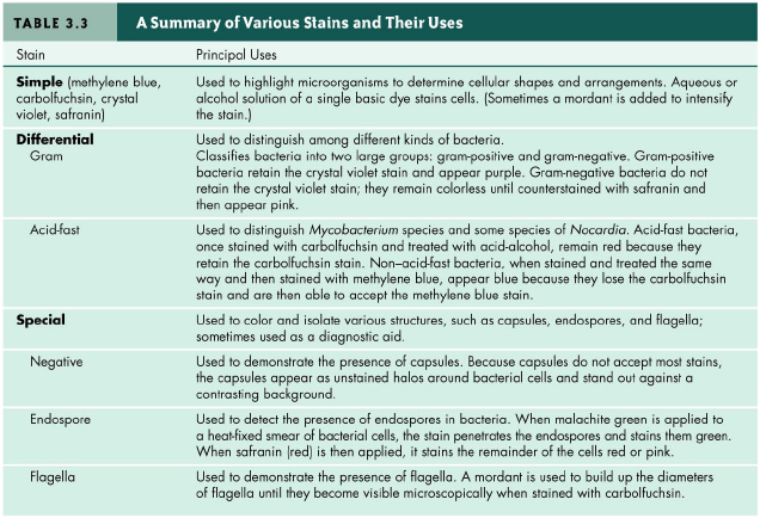
\includegraphics[width=\columnwidth]{A.imagenes/ACV-MICRO-Temp1}
	\caption[Resumen de las principales tinciones.]{Resumen de las principales tinciones. \textit{\textbf{Extraido de:}} \cite{Prescott2011}}
\end{figure}
    % SEC X - Citoplasma
     \chapter{Ultraestructura interna}
\section{Citoplasma}
El citoplasma está compuesto en un 70\% por agua, dónde se encuentran en solución coloidal una gran cantidad de macromoléculas u otras biomoléculas o bioelementos, con una presión oncótica u osmótica de 2 atmósferas. En el citoplasma, además, se encuentran presentes las enzimas bacterianas necesarias para su metabolismo y chaperonas (proteínas que ayudan a una proteína a alcanzar su plegamiento correcto). Así mismo se hallan proteínas con una función estructural, que dan forma a la célula, asimilándose al citoesqueleto de eucariotas. Algunas proteínas son:
\begin{itemize}[itemsep=0pt,parsep=0pt,topsep=0pt,partopsep=0pt]
	\item \textbf{FtsZ} (similar a la tubulina): tienen función en la división celular. Se encuentra en numerosas especies de Bacteria y Archaea.
	\item \textbf{MreB} (similar a la actina): dan la forma a la célula. Se encuentran en muchos géneros de bacilos.
	\item \textbf{Crescentina}: (similar a filamentos internos) dan forma a la célula. Se encuentra en especies como el \textit{Caulobacter crecentus}.
\end{itemize}

En el citoplasma se encuentran, además, orgánulos y el nucleoide. El nucleoide es el área del citoplasma donde se coloca el material genético (normalmente, un cromosoma circular) y plásmidos. Estos últimos son cadenas de DNA no vitales, pero que confieren al individuo ventajas adaptativas como resistencia a antibióticos, a daños or metales pesados o la incorporación al metabolismo de otros compuestos, como el plásmido \textit{Tol} (tolueno) de \textit{Pseudomona}. El cromosoma se encuentra, como en eucariontes, superenrollado, pero en este proceso no participan histonas.

Los ribosomas son el único orgánulo celular compartido con los tres dominios celulares. Con la misma función en todos los individuos, el bacteriano es de 70S, con una subunidad menor de 30S (compuesto por 21 proteinas y RNAr de 16S) y una mayor de 50S (compuesto por 34 proteínas y dos RNAr, uno de 23S y otro de 5S).

Otro tipo de orgánulo bacteriano son las inclusiones. Las inclusiones son gránulos de material orgánico o inorgánico envuelto o no por una membrana no unitaria (formadas por proteínas, lipoproteínas o glicoproteínas). Se generan, normalmente, bajo condiciones determinadas de crecimiento. Pueden ser:
\begin{itemize}[itemsep=0pt,parsep=0pt,topsep=0pt,partopsep=0pt]
	\item \textbf{Orgánicas}: de polisacáridos, de poli-$\beta$-hidroxialcano o cianoficina
	\item \textbf{Inorgánicas}: polifosfato o de azufre elemental. 
\end{itemize}

Algunos otros orgánulos no rodeados por membrana son las vesículas de gas, clorosomas, carboxisomas o magnetosomas. Como única excepción a la no presencia de orgánulos rodeados por membrana unitaria son los tilacoides de las cianobacterias.
\subsection{Inclusiones orgánicas}
Pueden ser:
\begin{itemize}[itemsep=0pt,parsep=0pt,topsep=0pt,partopsep=0pt]
	\item \textbf{Polisacarídicas}: de glucógeno (ósido de reserva animal) o de almidón (ósido de reserva vegetal). Ambos polímeros de glucosasirven como reservorio de carbono. Se comienzan a sintetizar cuando en el medio hay falta de nitrógeno. Cuando se restituye este elemento, se forman las proteínas con el carbono almacenado.
	\item De \textbf{poli-$\beta$-hidroxialcanoatos} (PHA): se encuentran entre ellos:
	\begin{itemize}[itemsep=0pt,parsep=0pt,topsep=0pt,partopsep=0pt]
		\item \textbf{Poli-$\beta$-hidroxibutirato} (PHB) polímero de ácido 3-hidroxibutírico unidos por enlace éster. Sirve como reservorio de carbono antes de la esporulación en \textit{Pseudomona} y \textit{Bacillus}.
		\item \textbf{Otros}, con función de bioplásticos (en el organismo vivo se utilizan como reserva de carbono), son copolímeros de poli-$\beta$-hidroxibutírico y poli-$\beta$-hidroxivalérico.
	\end{itemize}
	\item \textbf{Cianoficina}: presente únicamente en cianobacterias, como la Anaystis nidulans, son polímeros de aspartato con ramificaciones de arginina, unidos por enlaces peptídicos. Estas inclusiones, cuya generación se produce ante la falta en el medio de algún nutriente, se utilizan como reserva de carbono y nitrógeno.
\end{itemize}
\subsection{Inclusiones inorgánicas}
De las más conocidas son:
\begin{itemize}[itemsep=0pt,parsep=0pt,topsep=0pt,partopsep=0pt]
	\item \textbf{Inclusiones de polifosfato}: se dan en los géneros Lactobacillus y Spirilum. Se conocen también como gránulos de volutina o metacromáticos. Sirven de reserva de fosfato, produciéndose ante la falta de azufre.
	\item \textbf{Inclusiones de azufre}: observables en las bacterias verdes y en las quimiolitotrofas. En ambos casos, son acumulaciones temporales de azufre elemental que se da por un proceso lento de oxidación a sulfato ($SO_4^{2-}$). Se usa, en el caso de bacterias verdes, para obtener poder reductor, y en el caso de quimiolitotrofos, para obtener poder reductor y energía.
\end{itemize}
\subsection{Vacuolas de gas}
Estos orgánulos no presentan límite de membrana unitaria. Se hallan presentes en algunas procariotas, sobre todo acuáticas, siendo su función la de permitir al organismo moverse en la vertical hacia hábitats más propicios (más luz, nutrientes,$\dots$). Son agregados de un gran número de estructuras pequeñas huecas cilíndricas o fusiformes. Las cianobacterias con vesículas de gaspresentan una membrana especial, permeable a los gases, pero no al agua. De esta forma, al reducir su contenido en gas, desciende en profundidad; y al aumentar la cantidad de gas, ascienden.
    \part{Parasitología}
    % SEC I - Introducción
     \chapter{Introducción}
La parasitología es una rama de la Biología que estudia el parasitismo, realción ecológica entre dos seres de distinta especia (relación esterotípica o anisoespecífica) denominados hospedador, que proporciona un medio; y se relaciona con un parásito, ecuariota que desarrolla una dependencia metabólica con respecto al hospedador, mediante respuesta inmune. Entre hospedador y parásito se da una relación semántica y coevolutiva, por medio de adpatación. La relación de parasitismo puede prosperar o fracasar según el medio externo.

La parasitología sanitaria consiste en el estudio de los parasitismos que afectan al ser humano y que pueden tener repercusiones tanto para la salud individual que las padece como las poblaciones que les afecta. Mediante el estudio tanto de la morfología y biología de los parásitos como de las enferemedades que originan (patología y sintomatología) fijando las bases para su control.
\section{Definiciones}
\paragraph{Parásito}\footnote{\textit{al lado de la comida}}: a nivel biológico, animal que vive a expensas de otro. Forman en torno a dos tercios de la fauna del planeta. Comienzan a surgir a partir de organismos de vida libre, siendo los primeros los \textit{Unos} (tenias) en el Paleozoico, se expanden en número en el Cretácico y era Terciaria, dandose fenómenos de adaptaciones a tiempo real (amebas anfizoicas). De origen polifilético y evolutivo y temporal distintos, se clasifican:
\begin{itemize}[itemsep=0pt,parsep=0pt,topsep=0pt,partopsep=0pt]
	\item Según su habitat ojetivo:
	\begin{itemize}[itemsep=0pt,parsep=0pt,topsep=0pt,partopsep=0pt]
		\item \textbf{Fitoparásitos}: o plagas, son parásitos de plantas.
		\item\textbf{Zooparasitos}: parásitos de animales. Se subdividen:
		\begin{itemize}[itemsep=0pt,parsep=0pt,topsep=0pt,partopsep=0pt]
			\item \textbf{Ectoparásitos}: se localizan en el exterior. Pueden ser Hematófagos o no hematófagos.
			\item\textbf{Endoparásitos}: habitan en el interior del hospedador. Son:
			\begin{itemize}[itemsep=0pt,parsep=0pt,topsep=0pt,partopsep=0pt]
				\item Intestinales
				\item Subcutáneos
				\item Cavitarios (en el interior de órganso).
				\item Endocelulares
				\item Cenozoicos (en el interior del núcleo celular).
				\item Erraticos (Se mueven por el hospedador. Se pueden diferenciar de localización errática en tanto que alude a parásitos que no están en su hábitat habitual).
			\end{itemize}
		\end{itemize}
	\end{itemize}
	\item Según su tiempo de contacto:
	\begin{itemize}[itemsep=0pt,parsep=0pt,topsep=0pt,partopsep=0pt]
		\item \textbf{Permanente}: (piojos,$\dots$) lleva a cabo todo su ciclo biológico en un mismo hospedador: viviendo, creciendo y reproduciéndose en él.
		\item\textbf{Temporal}: (pulgas, etc.) el parásito vive en el ambiente del hospedado, próximo a él, pero sólo accede a este cuando precisa de cierta necesidad.
		\item\textbf{Estacional}: (mosquitos, $\dots$) sólo está presente en ciertas épocas del año.
		\item\textbf{Facultativos}: (\textit{Lucilia} spp, etc) el parásito puede vivier de forma libre o en forma parasitaria en alguno de los momentos de su vida.
	\end{itemize}
	\item Según los hospedadores intermedios en su ciclo vital:
	\begin{itemize}[itemsep=0pt,parsep=0pt,topsep=0pt,partopsep=0pt]
		\item \textbf{Monoxenos}: sólo presenta un hospedador.
		\item\textbf{Heteroxenos}: presenta varios hospedadores intermedios.
		\item\textbf{Poliheteroxenos}: presenta múchos hospedadores intermedios.
	\end{itemize}
	\item Según su especificidad:
	\begin{itemize}[itemsep=0pt,parsep=0pt,topsep=0pt,partopsep=0pt]
		\item \textbf{Estenoxeno}: (piojos, $\dots$) requieren unas condiciones muy concretas que provoca que se desarrollen sólo en una o muy pocas especies.
		\item\textbf{Eurixeno}: (\textit{Toxoplasma gondii}, etc.) tiene requerimientos poco específicos, por lo que puede desarrollarse en varias especies.
	\end{itemize}
\end{itemize}
\paragraph{Hospedador}: animal que proporciona un ambiente al parásito. Se clasifican:
	\begin{itemize}[itemsep=0pt,parsep=0pt,topsep=0pt,partopsep=0pt]
		\item \textbf{Definitivo}: hospedador en el que el parásito está en forma adulta y es capaz de reproducirse sexualmente.
		\item\textbf{Intermedio}: hospedador en el que el parásito está en forma larvaria y es capaz de reproducirse asexualmente.
		\item\textbf{Paraténica}: hospedador no necesario en el que el parásito permanece en un determinado estado y en el que no se reproduce, alargando su ciclo vital.
		\item\textbf{Reservorio}: hospedador vertebrado no humano que actúa como hospedador definitivo y supone una provisión de parásitos en la naturaleza (\textit{Leishmania} spp y el perro).
		\item\textbf{Vector}: hospedador invertebrado que actúa como hospedador intermedio\footnote{Se daría reproducción asexual} y como medio de transporte del parásito\footnote{Excepto \textit{Plasmodium} y el mosquito \textit{Anopheles}, ya que existe reproducción sexual en él} (\textit{Plasmodium} y la mosca tse-tse).
		\begin{itemize}[itemsep=0pt,parsep=0pt,topsep=0pt,partopsep=0pt]
			\item \textbf{Transmisor mecánico} o \textbf{portador}: hospedador donde no se da ningún tipo de reproducción, sólo dándose un movimiento entre dos puntos. Se usa con ectoparásitos.
		\end{itemize}
	\end{itemize}
\paragraph{Ciclo biológico}: conjunto de sucesos por los que pasa un parásito desde una fase determinada hasta que vuelve a esa fase. Existen distintos tipos:
\begin{itemize}[itemsep=0pt,parsep=0pt,topsep=0pt,partopsep=0pt]
	\item \textbf{Directo}: no existen hospedadores intermedios. Pueden ser:
	\begin{itemize}[itemsep=0pt,parsep=0pt,topsep=0pt,partopsep=0pt]
		\item \textbf{Saprozoico}: se transmite por agua o suelo, vehiculizado por estos.
		\item\textbf{No saprozoico}: se transmite de un hospedador a otro.
	\end{itemize}
	\item\textbf{Indirecto}: existen uno o varios hospedadores intermedios.
	\item\textbf{Facultativos}: Puede tener o no hospedadores intermedios.
	\item\textbf{Autoheteroxenos}: en el mismo hospedador se desarrolla todo el ciclo vital. (\textit{Trichinella} spp).
\end{itemize}
\paragraph{Ciclo epidemiológico}: referido a un hospedador, conjunto de sucesos por los que pasa un parásito al salir de un hospedador hasta que vuelve al mismo.
\paragraph{Agente etiológico o causal}: parásito, en cualquiera de sus formas, pudiendo darse que el mismo agente etiológico (parásito) esté en uno u otro estado dependiendo del hospedador. Se pueden llevar dos tipos de diagnósticos:
\begin{itemize}[itemsep=0pt,parsep=0pt,topsep=0pt,partopsep=0pt]
	\item \textbf{Directo}: búsqueda del parásito en el hospedador en cualquiera de las formas del ciclo vital de este.
	\item\textbf{Indirecto}: búsqueda de anticuerpos ante el parásito y de otros marcadores de respuesta inmune (más limitado por inespecificidad y poca antigenicidad).
\end{itemize}
\paragraph{Fuente de infección}: medio que lleva al parásito hasta el siguiente hospedador.
\paragraph{Vía de infección}: canal por el que llega el parásito al hospedador:
\begin{itemize}[itemsep=0pt,parsep=0pt,topsep=0pt,partopsep=0pt]
	\item Oral.
	\item Parenteral (a través de la piel y hacia la sangre).
	\item Congénita o placentaria.
	\item Venérea.
	\item Galactógena.
\end{itemize}
\section{Epidemiología}
\subsection{Introducción y definiciones}
\paragraph{Epidemiología}: ciencia que estudia el conjunto de conocimientos relativos a las enfermedades de las poblaciones humanas o comunidades más que la individuales. Estudia el conjunto de factores que determinan frecuencia y distribución de las enfermedades.
\paragraph{Prevalencia}: proporción de individuos que albergan el parásito (enfermos nuevos y antiguos) en una población determinada. Se expresa en porcentaje:
\begin{center}
	\begin{math}
		\mbox{Prevalencia} = \dfrac{\mbox{Nº parasitados}}{\mbox{Población total}} \cdot 100
	\end{math}
\end{center}
\paragraph{Incidencia}: casos nuevos de parasitosis en una población y periodo temporal. Se expresa como casos por 100 000 habitantes y año.

La prevalencia depende de la incidencia y duración de las parasitosis en tanto que alta incidencia y/o una enfermedad crónica aumnetan la prevalencia, mientras que parasitosis poco incidentes y/o de corta duración (rápida curación o alta mortalidad), la hacen descender.

\paragraph{Endemia/enzootia}: enfermedad constante en cieratas épocas y regiones por influencia de una causa local (gran número de hospedadores, etc.)
\paragraph{Hiperendemia/hiperenzootia}: endemia de alta prevalencia, originada por descontrol de una endemia.
\paragraph{Epidemia/Epizootia}: infección accidental transitoria que afecta al mismo tiempo y en la misma región a un gran número de individuos.
\paragraph{Pandemia}: epidemia que afecta a gran número de regiones.
\subsection{Factores determinantes}
Entre los factores que pueden determinar la distribuciónd e la enfermedad, se pueden agrupar en ambientales y derivados de la actividad humana.
\begin{itemize}[itemsep=0pt,parsep=0pt,topsep=0pt,partopsep=0pt]
	\item \textbf{Ambientales}:
	\begin{itemize}[itemsep=0pt,parsep=0pt,topsep=0pt,partopsep=0pt]
		\item \textbf{Bióticos}: se relacionan con la vegetación, que sirve de refugio a formas de vida libre o determina la presencia o no de ciertos hospedadores; y faunta, comunidades que viven juntos de especies distintas que se infectan a la vez y presencia de vectores en el ecosistema.
		\item\textbf{Abióticos}: del biotopo. Son:
		\begin{itemize}[itemsep=0pt,parsep=0pt,topsep=0pt,partopsep=0pt]
			\item \textbf{Climáticos}: como temperatura (altas temperaturas favorecen los ciclos de vida libre y los ciclos de transmisión por los artrópodos), viento (algunos vectores son incapaces de vivir en zonas con altos flujos de aire) o humedad (la alta humedad favorece los ciclos de vida libre al evitar la desecación y favorecer una gran vegetación que dé refugio y zonas sombrias que eviten la deshidratación del parásito).
			\item\textbf{Edáficas}: condicionan, la aridez o compactación del suelo, la supervivencia de ciclos de vida libre.
			\item\textbf{Hídricos}: el pH, turbidez, cantidad de oxígeno disuelto y materia orgánica, así como régimen de turbulencias, condicionan la vida de ciclos de vida libre y la posibilidad de infectar a un hospedador.
		\end{itemize}
	\end{itemize}
	\item\textbf{Antropogénicos}:
	\begin{itemize}[itemsep=0pt,parsep=0pt,topsep=0pt,partopsep=0pt]
		\item \textbf{Dependientes del nivel de desarrollo}: uso de suelos, disponibilidad de alimentos y agua potable, condiciones de vivienda, sanidad, escolaridad, etc.
		\item\textbf{Dependientes de la actividad humana}: construcción de grandes infraestructuras, colonización de áreas poco pobladas y deforestación, existencia de programas sanitarios, proximidad de animales (zoonosis), incremento del comercio y viajes, cambios demográficos (mayor población urbana que conlleva hacinamiento y escasez de servicios).
		\item\textbf{Existencia de conflictos armados}: dado que determina cambios ambientales y el desplazamiento forzoso de gran número de personas (hacinamiento, falta de servicios y salubridad).
	\end{itemize}
\end{itemize}

Todos estos factores determinan la distribución mayoritaria de las parasitosis en regiones tropicales: las condiciones de subdesarrollo determinan el desarrollo de parásitos que lastran el desarrollo económico.
\section{Respuesta inmune}
La respuesta inmune frente a los parásitos es muy compleja y rara vez suele ser tan sólida como la que se desarrolla frente a bacterias y virus\footnote{Excepto las leishmaniosis cutáneas que curan de forma espontánea y confieren inmunidad.}. Se puede llegar a cierta inmunidad ante gran cantidad de exposiciones, por ejemplo, los infectados por determinadas cepas son resistentes a cepas homólogas pero no a heterólogas.

Así mismo, en ciertas ocaciones, la respuesta inmune no sólo resulta inútil frente al parásito, sino que también es lesiva para el hospedador (inmunopatología), pudiendose dar fenómenos de alergias e hipersensibilidad (helmintos), destrucción de células sanas (hemolisis por antígenos adsorbidos de \textit{Plasmodium}), o formación de granulomas y fibrosis en órganos (\textit{Schistosoma}). Además, el propio parásito se ha dotado de estrategias para evitar o evadir la respuesta inmune.
\subsection{Mecanismos de evasión}
La respuesta inmunitaria se lleva a cabo mediante dos mecanismos:
\begin{itemize}[itemsep=0pt,parsep=0pt,topsep=0pt,partopsep=0pt]
	\item \textbf{Inmunidad natural innata}: es inespecífica (se desencadenan las mismas reacciones frente a distintos patógenos) y se produce en el momento de la entrada del parásito. Consiste en fagocitosis y reacciones inflamatorias de carácter humoral.
	\item\textbf{Respuesta adaptativa}: es de tipo específico (a distintos patógenos, distintos procesos), ligadas a ciertas células (linfocitos y células presentadoras de antígenos, leucocitos y anticuerpos), pudiendo ser de carácter celular, dependiendo de linfocitos T, o humoral, de linfocitos B. Actúan tiempo después de la entrada del parásito, se incrementan y persisten actuando por procesos complejos y únicamente frente a especias que indujeron su activación.
\end{itemize}

Dada la diferencia a nivel estructural, bioquímico, patogénico y de ciclo biológico, no se puede formar una respuesta inmune única. Aun así, según la localización del parásito, se pueden distinguir:
\begin{itemize}[itemsep=0pt,parsep=0pt,topsep=0pt,partopsep=0pt]
	\item Parásitos que viven en el entorno intracelular, generan una respuesta celular (protozoos).
	\item Parásitos que viven en el medios extracelular y en sangre, inducen respuestas humorales.
\end{itemize}

Los mecanismos de evasión de la respuesta inmune más frecuentes son:
\begin{itemize}[itemsep=0pt,parsep=0pt,topsep=0pt,partopsep=0pt]
	\item \textbf{Evasión del reconocimiento}: el parásito modifica de forma frecuente sus antígenos de superficie, volviendo ineficaces a los anticuerpos formados frente al parásito (tripanosomas africanos).
	\item\textbf{Enmascaramiento antigénico}: para evitar la dispersión del parásito por el organismo, esta los tapiza formando una membrana que impide el contacto con células inmunes y por ello, la respuesta inmune (quistes hidatídicos).
	\item\textbf{Encapsulamiento}: el parásito penetra en una célula, a la que modifica (formación de más retículo endoplásmico, creación de una cubierta,$\dots$) haciendola más fibrosa, como un quiste, y transformandola en una <<célula nodriza>> que protege al parásito (\textit{Trichinella}).
	\item\textbf{Modificación de la expresión antigénica}: según el estado de desarrollo, la fase del parásito en cada momento, tendrá distintos marcadores celulares (\textit{Plasmodium} varía sus antígenos en el momento de entrada al hepatocito, donde se reproduce asexualemnte, a su salida de éste y en el momento de entrada al eritrocito).
	\item\textbf{Adaptación a vivir en <<paraísos parasitarios>>}: el parásito vive en una región del organismo donde no llega la respuesta inmune (\textit{Toxoplasma gondii} y su colonización del Sistema Nervioso Central (SNC)).
	\item\textbf{Adaptación a vivir en células inmunes}: el parásito segrega enzimas que permiten vivir y multiplicarse en vacuolas líticas leucocitarias (\textit{Leishmania}).
	\item\textbf{Cubiertas}: posesión de un glicocálix o tegumento graso que protege frente a mecanismos citotóxicos de macrófagos y neutrófilos (helmintos).
\end{itemize}
\subsection{Inmunodiagnóstico}
Las características exigibles a cualquier prueba diagnóstica son:
\begin{itemize}[itemsep=0pt,parsep=0pt,topsep=0pt,partopsep=0pt]
	\item \textbf{Sensibilidad}: capacidad de detección de casos positivos ante cantidades mínimas de marcador.
	\item\textbf{Especificidad}: capacidad de detección de casos negativos, eliminando reacciones cruzadas.
	\item\textbf{Reproducibilidad}: capacidad de que tantas veces se repita el experimento, el resultado no varie.
	\item Facilidad de realización, rapidez y bajo coste.
\end{itemize}
A estas características se le ha de añadir la definición de un título límite del marcador que indique la presencia de parasitosis.

El diagnóstico inmunológico es un tipo de diagnóstico indirecto que complementa al directo o morfológico, pero no lo sustituye. De gran utilidad cuando el parásito no es fácilmente localizable o no hay formas de eliminación. Existen varios tipos:
\begin{itemize}[itemsep=0pt,parsep=0pt,topsep=0pt,partopsep=0pt]
	\item Detección de antígenos específicos.
	\item Detección de antígenos solubles.
	\item Detección de inmunocomplejos circulantes.
	\item Exploración de inmunidad mediada por células (citoquinas, interleuquinas, interferones, linfoblastos, $\dots$)
\end{itemize}
Las técnicas más usadas son:
\begin{itemize}[itemsep=0pt,parsep=0pt,topsep=0pt,partopsep=0pt]
	\item \textbf{Reacciones de precipitación}: inmunoelectroforesis, inmunodifusióon radial (Mancini), doble difusión, contrainmunoelectroforesis, etc.
	\item\textbf{Reacciones de aglutinación}: aglutinación directa, hemoaglutinación, aglutinación con látex, Pentonita.
	\item\textbf{Marcadores}: inmunofluorescencia, enzimoimnunoanálisis (ELISA y variantes), radioinmunoanálisis.
\end{itemize}
\section{La enfermedad parasitaria}
En el caso del parasitismo, de la interacción hospedador-parásito, pueden darse 4 supuestos:
% Please add the following required packages to your document preamble:
% \usepackage{multirow}
\begin{table}[H]
	\begin{tabular}{cccc}
		&  & \multicolumn{2}{c}{Hospedador} \\
		&  & \multicolumn{1}{c|}{Vive} & Muere \\ \cline{3-4} 
		\multirow{2}{*}{Parásito} & \multicolumn{1}{c|}{Vive} & \multicolumn{1}{c|}{\begin{tabular}[c]{@{}c@{}}Parasitismo próspero: parásito vive y\\ hospedador lo tolera\end{tabular}} & \begin{tabular}[c]{@{}c@{}}Parásito se establece pero \\ mata al hospedador\end{tabular} \\ \cline{2-4} 
		& \multicolumn{1}{c|}{Muere} & \multicolumn{1}{c|}{\begin{tabular}[c]{@{}c@{}}Parásito se establece y\\ el hospedador lo mata\end{tabular}} & Parásito no se establece
	\end{tabular}
	\caption{Cuadro de relaciones de parasitismo. \label{table:PARASIT:EnferParasRelac}}
\end{table}

En una relación de parasitismo se define:
\begin{itemize}[itemsep=0pt,parsep=0pt,topsep=0pt,partopsep=0pt]
	\item \textbf{Infección inaparente}: los parásitos viven en el hospedador sin causar daño aparente durante periodos largos o recidivas(en el caso de los helmintos, sólo se ven síntomas en caso de que gran número de ellos estén; o en el caso del paludismo, las recidivas cada 48 o 72 horas).
	\item\textbf{Portador sano}: estado del portador durante la infección inaparente, no manifestando signos ni síntomas, dado que el daño tisular se realiza a la misma velocidad de recuperación, con posibilidad de transmisión del parásito.
	\item\textbf{Parasitismo}: relación en equilibrio entre parásito y hospedador sano o portador.
	\item\textbf{Parasitosis}: enfermedad parasitaria provocada por la ruptura del equilibrio del parasitismo. Aun sin daños en el hospedador, el parásito es casi siempre un patógeno.
	\item\textbf{Patogenicidad}: capacidad de un parásito de producir daño a un hospedador, generando una enfermedad.
\end{itemize}

Los parásitos, como todo ser vivo de la escala zoológica, tiene un nombre genérico y otro específico que lo identifica, escribiendos siempre en cursiva o subrayado, el latín y con el género empezando en mayúscula. Las enfermedades producidas por los parásitos se nombran como el género del parásito que la produce acabado en <<-\textit{osis}>> (o -\textit{asis} o -\textit{iasis}). En cuanto a las parasitosis, se clasifican:
\begin{itemize}[itemsep=0pt,parsep=0pt,topsep=0pt,partopsep=0pt]
	\item \textbf{Antroponosis}: parasitósis exclusivas del ser humano.
	\item\textbf{Zoonosis}: parasitosis exclusivas de animales no humanos.
	\item\textbf{Antropozoonosis}: parasitosis que afectan por igual a todos los animales, incluidos humanos.
\end{itemize}
\subsection{Factores condicionantes de la patogenia}
Se pueden distinguir entre factores intrínsecos (del parásito) y extrínsecos (del hospedador):
\begin{itemize}[itemsep=0pt,parsep=0pt,topsep=0pt,partopsep=0pt]
	\item \textbf{Intrínsecos}:
	\begin{itemize}[itemsep=0pt,parsep=0pt,topsep=0pt,partopsep=0pt]
		\item \textbf{Grado de infección}: número de parásitos que se asientan en el hospedador. Cuanto mayor sea, más patógeno será el parásito.
		\item\textbf{Capacidad de multiplicación del parásito}.
		\item\textbf{Virulencia}: capacidad del parásito de producir daño.
		\item\textbf{Localización del parásito}: depende de la localización puntual del parásito en caso de migrar, dandose mayor estimulación antigénica en sangre y tejidos que en el intestino.
	\end{itemize}
	\item\textbf{Extrínsecos}:
	\begin{itemize}[itemsep=0pt,parsep=0pt,topsep=0pt,partopsep=0pt]
		\item \textbf{Edad}.
		\item\textbf{Estado funcional}: embarazo o lactancia exacerban los síntomas y daños.
		\item\textbf{Estado nutricional}.
		\item\textbf{Estado inmunitario}.
	\end{itemize}
\end{itemize}

Así, se definen los siguientes términos:
\begin{itemize}[itemsep=0pt,parsep=0pt,topsep=0pt,partopsep=0pt]
	\item \textbf{Periodo de incubación}: periodo de tiempo transcurrido entre el contagio y la aparición de síntomas y signos.
	\item\textbf{Periodo prepatente}: tiempo que transcurre desde el contagio hasta la eliminación de formas parasitarias de transmisión.
	\item\textbf{Periodo patente o de estado}: periodo de tiempo en elq ue la enfermedad es manifiesta y se eliminan formas de diseminación.
	\item\textbf{Periodo postpatente}: tiempo de ausencia de sintomatología y descenso de formas de eliminación.
	\item\textbf{Etiología}: causa de la enfermedad.
	\item\textbf{Patogénia}: dinámica de la enfermedad, estudio de la interacción parásito-hospedador.
	\item\textbf{Sintomatología}: conjunto de signos\footnote{Manifestaciones cuantificables y objetivas.} y síntomas\footnote{Manifestaciones subjetivas.} de la enfermedad. En el caso de las parasitosis, la sintomatología, por ser vaga y fácilmente confundible, no es definitoria de enfermedad, necesitando confirmar diagnósticos mediante laboratorio.
\end{itemize}
\subsubsection{Acción patogénica del parásito}
Los parasitos pueden causar daño al hospedador mediante distintas acciones:
\begin{itemize}[itemsep=0pt,parsep=0pt,topsep=0pt,partopsep=0pt]
	\item \textbf{Mecánicas}: según el volumen, número y localización de los parásitos pueden ser:
	\begin{itemize}[itemsep=0pt,parsep=0pt,topsep=0pt,partopsep=0pt]
		\item\textbf{De presión}: quistes hidatídicos, cisticercosis cerebrales, etc.
		\item\textbf{De bloqueo}: filarias linfáticas, ascaris intestinales, $\dots$
	\end{itemize}
	\item\textbf{Traumática}: ruptura de tejidos por penetración, migración o asentamiento del parásito.
	\item\textbf{Expoliadora}: sustracción de nutrientes de tipo general o específico.
	\item\textbf{Toxicológica}: dada por sustancias producidas por el vector (hinchazón ante la picadura, etc.) o metabolitos del parásito (sarcocistina, un neurotóxico del parásito \textit{Sarcocystis}).
	\item\textbf{Vehiculadora}: transporte de gérmenes de un sitio a otro (infección secundaria), pudiendo ser desde el medio externo o interno.
	\item\textbf{Estimulación de reacciones hísticas}: inflamaciones, encapsulamiento fibrosos o eosinofilia (helmintos). Resultan en:
	\begin{itemize}[itemsep=0pt,parsep=0pt,topsep=0pt,partopsep=0pt]
		\item\textbf{Hipertrofia}: aumento del tamaño del órgano.
		\item\textbf{Hiperplasia}: aumento de la función del órgano.
		\item\textbf{Neoplasia}: aumento de la división celular en el órgano.
	\end{itemize}
\end{itemize}
\subsection{Importancia socioeconómica}
Pese al gran porcentaje de población (33 \%) que sufre estas enfermedades, son enfermedades desatendidas.
\begin{multicols}{2}
	Las parasitosis tiene efecto a nivel económico en tanto pérdida de mano de obra (incapacidad o muerte), como aumento del gasto sanitario y pérdidas por absentismo laboral, así como de perdida de productividad en el caso de las zoonosis, por muerte del ganado y pérdida de fuerza de tiro. El aumento de las zoonosis también genera un aumento de las antropozoonosis, especialmente virulentas en ninños (con mayor contacto y menor desarrollo inmune), que lastra el aumento de mano de obra.
	\columnbreak
	\begin{figure}[H]
		\centering
		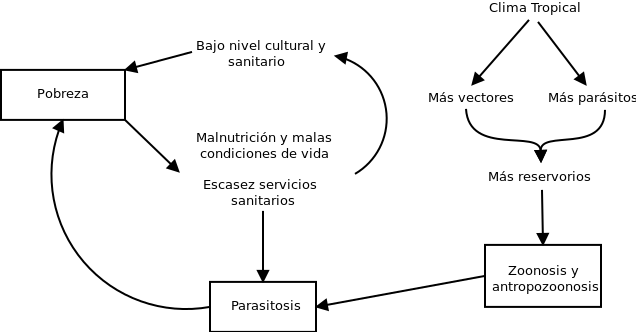
\includegraphics[width=0.9\columnwidth]{A.imagenes/ACV-BioSan-Parasit-ImportSocioecon}
		\caption[Repercusiones de las parasitosis]{Esquema de las repercusiones socioeconómicas de las parasitosis.\label{fig:PARASIT:ConsecSocioecon}}
	\end{figure}
\end{multicols}
Las antropozoonosis tienden a cronificarse, cursando de forma asintomática (portadores sanos), y requieren terapia prolongada, que por su elevado coste (medicamento o administración), sólo se da adultos y no se completa, o se dan de forma adulterada, generando resistencias.

Las antropozoonosis suelen provocar rechazo social por confusión con otras patologías (\textit{Oncocerca volvulas} provoca dermatitis asemejan a la lepra), son incapacitantes, se asocian con profesiones o prácticas con rechazo social o manifestaciones que se asocian a prácticas calificadas como negativos o pensamientos magico-religiosos negativos o problemas de nutrición. Acaban, en infantes, generando retraso físico y mental. La mayor libertad sexual aumentó las parasitosis por vía venerea y ciertas inmunodepresiones (SIDA,etc.) y el aumento de intercambio de población y mercancías han aumentado la propagación de las parasitosis. El rechazo social incrementa el no tratamiento y con ello, contagio y propagación. Por ello, en tanto freno a la inversión, pérdida de productividad y aumento del gasto, las parasitosis generan subdesarrollo y este, retroalimenta el ciclo: la salud es necesaria para acabar con la pobreza.
\begin{figure}[H]
	\centering
	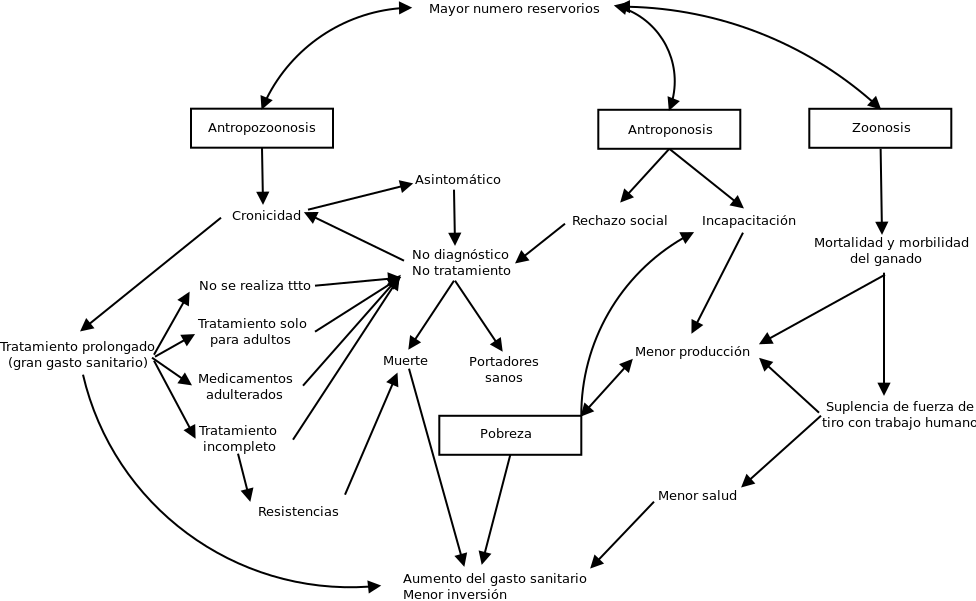
\includegraphics[width=\columnwidth]{A.imagenes/ACV-BioSan-Parasit-ImportSocioecon2}
	\caption[Consecuencias ampliadas de las parasitosis]{Consecuencias socioeconómicas que favorecen las parasitosis y efectos de estas.\label{fig:PARASIT:ConsecSocioecon2}}
\end{figure}
    % SEC I - Protozoos
     \chapter{\textit{Phylum} Protozoa}
\section{\textit{Sarcodinia}}
\subsection{\textit{Entamoeba histolítica}}
Ameba cosmopolita, aunque con gran incidencia en regiones tropicales y subtropicales (prevalencia de hasta el 40 \%). Provoca, entre otras patologías, la \textit{diarrea del viajero}. Afecta a 10 millones de personas en todo el mundo, causando unas 100000 muertes anuales, siendo el 80 \% de los infectados portadores sanos. No obstante, la facilidad de confusión con \textit{Entamoeba dispar}, otra ameba comensal y no patógena, hace que los datos no sean del todo exactos. Se diferencian mediante técnicas de laboratorio (moleculares y bioquímicas).
\subsubsection{Morfología}
\textit{E. histolytica} presenta dos formas: una patógena (trofozoito) y otra de resistencia (quiste).
\begin{itemize}[itemsep=0pt,parsep=0pt,topsep=0pt,partopsep=0pt]
	\begin{multicols}{2}
		\item \textbf{Trofozoito}: (figura \ref{fig:PARASIT:EHistolyticaMorf}, derecha) sin forma constante por la emisión de pseudópodos, se meuve sobre superficies de forma directa por la emisión de lobópodos. Presenta dos zonas: ectoplasma (externo, de aspecto hialino y sin orgánulos celulares) y endoplasma (interno, rugoso y con orgánulos celulares). Tiene un núcleo con un nucleolo central y heterocromatina dispuesta perifericamente. En el citoplasma no se hallan mitocondrias, retículo endoplásmico o aparato de Golgi, pero sí polirribosomas, microtúbulos, glucógeno $\alpha \mbox{ o } \beta$ y vacuolas alimentarias con eritrocitos en degradación.
		\columnbreak
		\begin{figure}[H]
			\centering
			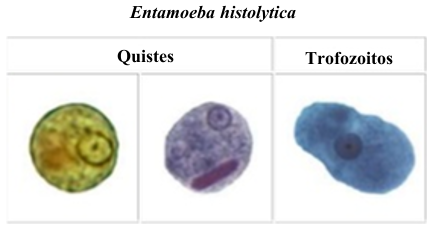
\includegraphics[width=0.9\columnwidth]{A.imagenes/ACV-BioSan-Parasit-EHistolyticaMorf}
			\caption[Quistes de \textit{E. Histolytica}]{\textit{E. histolytica} en sus dos morfologías: la de resistencia o quiste, con 2 ó 4 núcleos (inmaduros y maduros, respectivamente); y la forma patógena que se puede hallar en tejido.\label{fig:PARASIT:EHistolyticaMorf}}
		\end{figure}
	\end{multicols}
	\item\textbf{Quistes}: (figura \ref{fig:PARASIT:EHistolyticaMorf}, central e izquierda) capaces de soportar las condiciones externas, es la forma de contagio. De forma esférica, presenta una membrana gruesa que lo protege y da forma. En su interior presenta 2 ó 4 núcleos, según su madurez (2, inmaduro; 4, maduro), acúmulos de glucógeno y unos cuerpos cromatoides en forma de huso (figura \ref{fig:PARASIT:EHistolyticaMorf}, central).
\end{itemize}
\begin{table}[H]
	\begin{tabular}{c|ccc}
		\rowcolor{black}&\textcolor{white}{\textit{\textbf{E. histolytica}}}&\textcolor{white}{\textbf{\textit{E. dispar}}}&\textcolor{white}{\textit{\textbf{E. coli}}}\\
		Tamaño quiste ($\mu m$)&15 a 20&15 a 20&15 a 50\\
		\rowcolor{hiperlightgray}Núcleos (en madurez)&4&4&8\\
		Nucleolo&Central&Central&Excéntrico\\
		\rowcolor{hiperlightgray}Cromatina&Uniforme&Uniforme&Irregular\\
		Cuerpos cromatoides& Bordes Redondeados&Bordes Redondeados&Bordes Astillados\\
		\rowcolor{hiperlightgray}Patogenicidad&Sí (hematófoga y extraintestinal)&No&No\\
		\hline
	\end{tabular}
	\caption{Diferencias morfológicas entre las principales \textit{Entamoebas} intestinales humanas.\label{table:PARASIT:EHistolyticaDiferMorf}}
\end{table}
\subsubsection{Ciclo biológico}
\begin{multicols}{2}
	Se trata de un ciclo directo, ocurriendo todo en un mismo hospedador. El punto de inicio del ciclo se da con la ingesta de agua y/o comida infectada con los quistes de \textit{E. histolytica}, ya sean maduros o inmaduros. Los quistes, por su tegumento, resisten los ácidos estomacales, produciendos la exquistación ante el pH neutro del intestino delgado. Se da una multiplicación nucleolar que resulta en un trofozoito multinucleado (con hasta 8 núcleos) que sufre una rápida citocinesis, obteniendo trofozoitos maduros que avanzan por el intestino empujados por el bolo alimenticio. A medida que descienden por el intestino, la menor humedad promueve el proceso de enquistación, formando un prequiste (se redondea y forma una cubierta glucídica que es la cubierta quística y se desorganiza el nucleolo), generando un prequiste con un núcleo y tras la cariocinesis, un quiste inmaduro, con la generación de los cuerpos cromatoides. La segunda cariocinesis da lugar a la maudración del quiste y pérdida de los cuerpos cromatoides. En las heces se expulsan todas las formas de estas amebas (los trofozoitos pueden desarrollar canales y proteínas que los unen a la pared intestinal y permiten invadirla), pero solo sobrevivirán los quistes. Existe también una via de infección por prácticas sexuales (oral o anal).
	\columnbreak
	\begin{figure}[H]
		\centering
		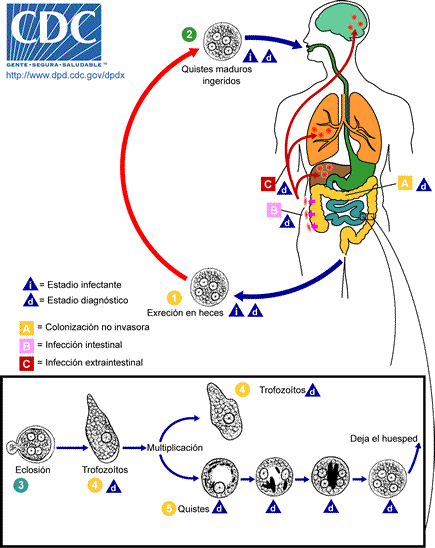
\includegraphics[width=\columnwidth]{A.imagenes/ACV-BioSan-Parasit-EHistolyticaCbios}
		\caption[Ciclo biológico de \textit{E. histolytica}.]{Ciclo biológico de \textit{E. histolytica}.\\Vehículo: agua o comida (directo no saprozoico).\\Vía: oral.\\Agente: quistes. \label{fig:PARASIT:EHistolyticaCBios}}
	\end{figure}
\end{multicols}
\subsubsection{Control}
\begin{itemize}[itemsep=0pt,parsep=0pt,topsep=0pt,partopsep=0pt]
	\item Saneamiento de aguas residuales
	\item Profilácticos.
	\item Medidas higienicas y lavado de alimentos (lejía alimentaria).
\end{itemize}
\subsubsection{Patología}
El periodo de incubación es de 2 a 21 días, el prepatente de 2 a 7 y el patente se puede extender durante años.
\begin{itemize}[itemsep=0pt,parsep=0pt,topsep=0pt,partopsep=0pt]
	\item\textbf{Disenteria\footnote{En griego: \textit{Muchas deposiciones}} amebiana} o \textbf{Amebiosis intestinal}: se produce en la fase inicial en el intestino. Los trofozoitos se adsorben en la mucosa y mediante enzimas, producen una actividad lítica del tejido, formando una úlcera <<en cuello de botella>>, reproduciendose en ella en forma de <<panal de abeja>>. Si la ulceración llega a la submucosa, pueden ir a localizaciones secundarias (enfermedad extraintestinal).
	\item\textbf{Amebomas}: granulomas en el cólon (sólo en el 1 \% de los casos, y en Latinoamérica).
	\item\textbf{Abcesos extraintestinales}: a través del torrente sanguineo, las amebas colonizan el SNC, hígado o lo hacen a través de las pleuras (con ulceraciones intestinales sangrantes).
\end{itemize}
\subsubsection{Sintomatología} 
\begin{itemize}[itemsep=0pt,parsep=0pt,topsep=0pt,partopsep=0pt]
	\item\textbf{Lesiones intestinales}: dolor abdominal; diarrea sanguinolienta , abunudante y con mucus; fiebre alta y dolor de cabeza. Si la amebiosis prospera, se pude producir paro cardiaco por agotamiento o peritonitis por perforación intestinal.
	\item\textbf{Lesiones extraintestinales}: se forman abcesos (formación con amebas externas e internas con tejido necrótico) en cerebro, bajo el nombre de meningoencefalitis amebiana secundaria; o abcesos hepáticos, en piel, pulmón y pene.
\end{itemize}
\subsubsection{Diagnosis}
\begin{itemize}[itemsep=0pt,parsep=0pt,topsep=0pt,partopsep=0pt]
	\item\textbf{Etiológico}: mediante examen de heces, distinguiendo a comensales como \textit{Entamoeba coli} o \textit{E. dispar}, esta última mediante técnicas moleculares.
	\item\textbf{Inmunodiagnóstico}: de escasa sensibilidad en caso de no haber amebas en sangre. Se hace mediante IFI, inmunohemoaglutinación, o ELISA (sensibilidad del 95 \% en casos extraintestinales, 70 \% en intestinales y 10 \% en asintomáticos; IgM dan positivo el 64 \% de las veces).
	\item\textbf{PCR}: permite descartar a \textit{E. dispar}.
\end{itemize}
\newpage
\section{Amebas anfiozoicas}
Las amebas anfizoicas\footnote{En griego: \textit{Ambas vidas} [libre y parasitaria].} siguen un ciclo biológico facultativo pudiendo vivir de forma exozoica como amebas de vida libre o endozoica como parasitos unicelulares. Su ciclo parasitario surge de una penetración accidental en el hospedador. Actualmente, se está dando un proceso de adaptación al parasitismo. Producen, por llevar acabo su acción primaria en el cerebro, una meningoencefalitis amebiana primaria que, por confusión en el diagnóstico y la falta de coevolución, resulta ser virulenta y mortal. Los géneros que afectan al ser humano son \textit{Naegleria fowleri}, \textit{Acanthamoeba cultbersoni}, \textit{Balamuthia} y \textit{Sappinia}; siendo las dos primeras las más incidentes.
\subsubsection{Morfología}
\begin{multicols}{2}
	\subsection{\textit{Naegleria fowleri}}
	Presenta tres estados. En todos los casos, el núcleo sólo es visible con microscopio de contraste de fases.
	\begin{itemize}[itemsep=0pt,parsep=0pt,topsep=0pt,partopsep=0pt]
		\item\textbf{Trofozoito ameboide}: muy activos metabolomicamente, no tienen forma constante por la emisión de pseudópodos, por los que se mueven por las superficies. Presentan un ectoplasma externo, hialino y sin orgánulos celulares; y un endoplasma interno, rugoso, con orgánulos celulares y el núcleo en posición central.
		\item\textbf{Trofozoito flagelado}: resultante del proceso a un medio líquido de las formas ameboides, o por medios poco ricos. Temporal, no presenta ectoplasma. Es ovalado, con endoplasma típico y dos flagelos polares.
		\item\textbf{Quistes}: capaces de soportar condiciones extremas, son redondeados, esféricos, con una membrana externa gruesa con perforaciones, núcleo central y endoplasma denso.
	\end{itemize}
	\columnbreak
	\subsection{\textit{Acanthamoeba cultbersoni}}
	Presenta dos estados:
	\begin{itemize}[itemsep=0pt,parsep=0pt,topsep=0pt,partopsep=0pt]
		\item\textbf{Trofozoito}: poco activo metabolicamente, sin forma constante, presenta un único núcleo y dos zonas diferenciadas: un ectoplasma externo, hialino y sin orgánulos celulares; y un endoplasma interno, rugoso, con orgánulos celulares. Tiene dos tipos de prolongaciones: filópodos, o pseudópodos espinosos, y acantopodinas, o lobópodos redondeados.
		\item\textbf{Quistes}: presenta las mismas estructuras del trofozoito (ectoplasma, endoplasma y un núcleo poco visible), carece de prolongaciones. El endoplasma tiene conformaciones poliédricas.
	\end{itemize}
\end{multicols}
\begin{figure}[H]
	\centering
	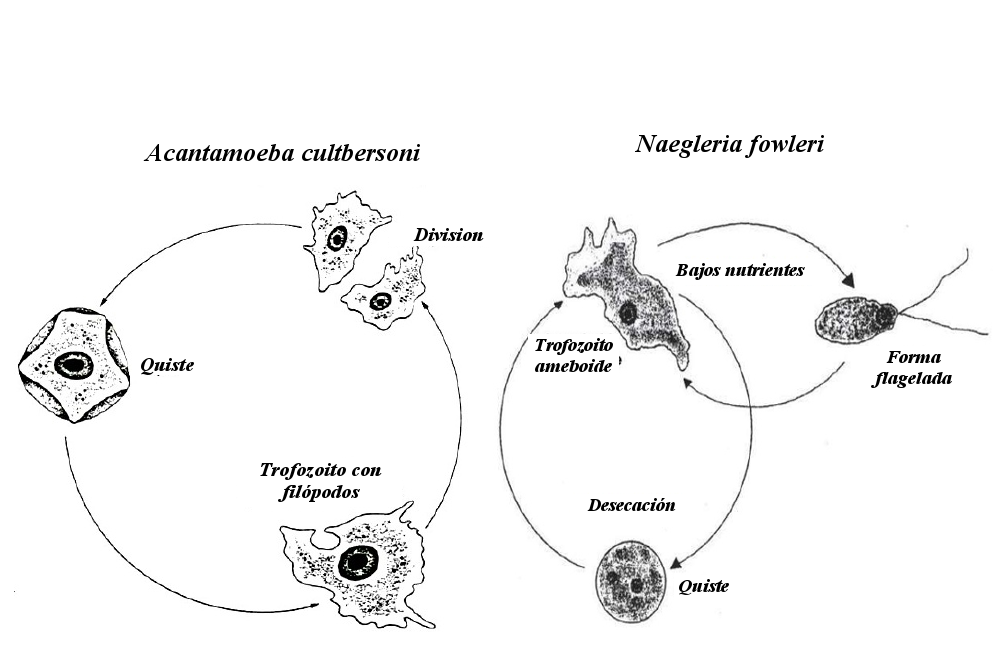
\includegraphics[trim=0 0.1cm 0.01cm 4cm,clip,width=0.55\columnwidth]{A.imagenes/ACV-BioSan-Parasit-AAnfizMorf}
	\caption[Morfología y ciclo vital \textit{N. fowleri} y \textit{A. cultbersoni}]{Morfología y ciclo vital libre de las dos amebas anfizoicas más comunes: \textit{N. fowleri} y \textit{A. cultbersoni}.\label{fig:PARASIT:AAnfizMorf}}
\end{figure}
\subsubsection{Ciclo biológico}
Estas amebas se hallan presentes en el fondo de lagos y pozas (\textit{Naegleria} es capaz de vivir en aguas a 50º C y \textit{Acanthamoeba} vive en filtros de aire con \textit{L. pneumophila}). Estas amebas, por medio de turbulencias, ascienden a la superficie. Por aerosoles, estas amebas ingresan en la cavidad nasal del hospedador, llegando a su epitelio olfativo. De éste, siguiendo sus vías axonales, viajan al lóbulo olfativo, extendiendose por el encéfalo a la par que se multiplican asexualmente. En el caso de \textit{A. cultbersoni} puede llevar consigo a \textit{L. pneumophila}. Es capaz a su vez de introducirse por heridas en la piel o por la córnea.
\subsubsection{Control}
\begin{itemize}[itemsep=0pt,parsep=0pt,topsep=0pt,partopsep=0pt]
	\item Evitar bañarse en aguas no controladas.
	\item Cloración y salinización (>0.7 \%) de aguas.
	\item Adición de poliheximida al 2 \% para líquidos de lentillas.
\end{itemize}
\begin{figure}[H]
	\centering
	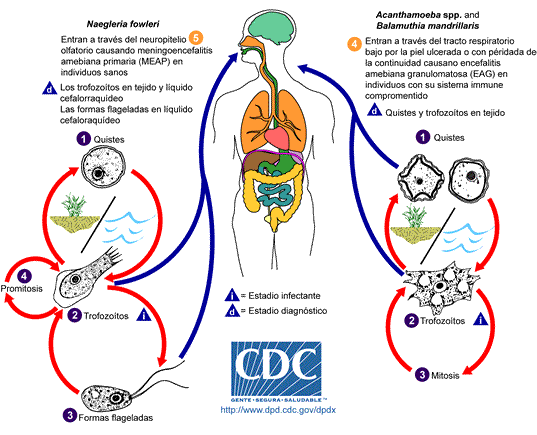
\includegraphics[width=0.65\columnwidth]{A.imagenes/ACV-BioSan-Parasit-AAnfizCbios}
	\caption[Ciclos biológicos de \textit{N. fowleri} y \textit{A. cultbersoni}.]{Ciclos biológicos de \textit{N. fowleri} y \textit{A. cultbersoni}. Vehículo: aerosoles infectados (directo no saprozoicos), Vía: nasal, parenteral u ocular, Agente: Trofozoito.\label{fig:PARASIT:AAnfizCBios}}
\end{figure}
\subsubsection{Patología}
\begin{itemize}[itemsep=0pt,parsep=0pt,topsep=0pt,partopsep=0pt]
	\item\textbf{Meningoencefalitis amebiana primaria}: su periodo de incubación es de 1 a 3 días, o raramente de 7 a 14 días. La principal acción del parásito es una acción traumática de bloqueo, generando focos necróticos en el encéfalo. La sintomatología comienza con el comienzo de las divisiones y es facilmente confundible con una meningitis bacteriana: cefaleas, fiebre alta, nauseas, vómitos, rigidez de la nuca, encefalitis, creación de zonas necróticas y de consistencia blanda, meninges purulentas y congestión del bulbo olfativo. La muerte llega, en el 95 \% de los casos, a los 4 o 6 días.
	\item En el caso de \textit{A. cultbersoni}, causa:
	\begin{itemize}[itemsep=0pt,parsep=0pt,topsep=0pt,partopsep=0pt]
		\item\textbf{Encefalitis amebiana granulomatosa}: de desarrollo lento (periodo de incubación desconocido), se produce cuando el parásito se introduce por heridas y se distribuye por sangre. Allí donde se multiplica el parásito, forma una membrana. Los síntomas: afección nerviosa en varios puntos, dolor de cabeza insidioso, fiebre esporádica, ataxia y desorientación.
		\item\textbf{Queratinitis}: se produce ante situaciones de inmunocompromiso, traumas epiteliales en la córnea y agua de limpieza de lentillas contaminada con amebas. Se produce una destrucción de la córnea por inflamación, ulceración y perforación. Sus síntomas se confunden con infecciones por infecciones por herpes o bacterias: opacidad de la córnea, iritis, irritación ocular, lagrimeo excesivo, dolores agudos y pérdida de visión.
	\end{itemize}
\end{itemize}
\subsubsection{Diagnóstico}
\subsubsection{\textit{Naegleria fowleri}}
\begin{itemize}[itemsep=0pt,parsep=0pt,topsep=0pt,partopsep=0pt]
	\item\textbf{Clinico}: buscando síntomas y antecedentes del paciente.
	\item\textbf{Etiológico}: en líquido cefalorraquidio se puede encontrar viva y movil con Giemsa y tinciones de Wright. Cultivable en agar \textit{E. coli}.
	\item\textbf{Inmunológico}: Inmunofluorescencia o inmunoperoxidasa en necropsias.
	\item\textbf{PCR}.
\end{itemize}
\subsubsection{\textit{Acanthamoeba culbertsoni}}
\begin{itemize}[itemsep=0pt,parsep=0pt,topsep=0pt,partopsep=0pt]
	\item\textbf{Etiológico}: identificada en biopsias cutáneas o cerebrales (granulomas) o mediante su cultivo a 22 y 37 C
	\item\textbf{Inmunológico}: mediante IFI o ELISA con antígenos extraidos de tejido fijados en formol.
	\item\textbf{PCR}.
\end{itemize}
\newpage
\section{Ciliados}
\subsection{\textit{Balantidium coli}}
La balantidiosis es una enfermedades transmitidas por parásitos protozoarios intestinales relativamente comunes y de amplia distribución mundial. De ciclos y sintomatología parecida \textit{Giardia lambia}, son relativamente distantes en cuanto a su taxonomía.
\subsubsection{Morfología}
\textit{Balantidium coli} es un protozoo cosmopolita ciliado (siendo el único parásito de humanos ciliado). Tiene dos formas:
\begin{itemize}[itemsep=0pt,parsep=0pt,topsep=0pt,partopsep=0pt]
	\item \textbf{Trofozoito}: mide entre 30 y 300 $\mu$m de largo y entre 25 y 120 $\mu$m de ancho. En su parte externa presenta una película de la que surgen cilios en filas longitudinales, que, en el citoplasma, se interconectan en una estructura denominada cinetodesma. Esta estructura se encarga de la organización sincrónica del movimiento, conociéndose al total de la estructura que realiza la función como infraciliatura. Presenta dos núcleos, un macronúcleo (grande, de forma de J o judía, relacionada con funciones tróficas) y un micronúcleo (pequeño, situado en la concavidad del macronúcleo, relacionado con funciones de reproducción). Tiene en el citoplasma dos vacuolas contráctiles. Así mismo, es relevante una estructura, el citostoma. Esta estructura es una invaginación en forma de embudo no ciliada de este protozoo por la que introduce el alimento. Se compone de una abertura externa (peristoma), que se continúa con un conducto (citofaringe) que acaba en un ciego junto a la vacuola alimentaria. En el polo contrario se halla el citopigio, por donde se exocitan los desechos.
	\item \textbf{Quiste}: de un tamaño de entre 45 y 75 $\mu$m de diámetro, son estructuras esféricas recubiertas de una pared resistente. Tras esa pared se descubre una célula muy similar al trofozoito: sin citostoma, ciliada y con los dos núcleos.
\end{itemize}
\begin{multicols}{2}
	\begin{figure}[H]
		\centering
		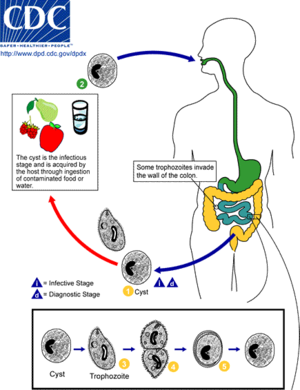
\includegraphics[width=\columnwidth]{A.imagenes/ACV-BioSan-Parasit-BcoliCBios}
		\caption[Ciclo biológico de \textit{B. coli}]{Ciclo biológicos de \textit{B. coli}. Vehículo: comida y agua infectadas, Vía: oral, Agente: Quiste.\label{fig:PARASIT:BColiCBios}}
	\end{figure}
	\columnbreak
	\vspace*{5.4cm}
	\begin{figure}[H]
		\centering
		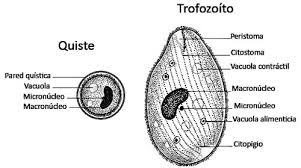
\includegraphics[width=\columnwidth]{A.imagenes/ACV-BioSan-Parasit-BcoliMorf}
		\caption[Morfología de \textit{B. coli}]{Morfología de \textit{B. coli}. A la izquierda, el quiste con sus secciones; a la derecha, la forma parasitaria intestinal.\label{fig:PARASIT:BColiMorf}}
	\end{figure}
\end{multicols}
\subsubsection{Ciclo biológico}
La localización de \textit{B. coli} es, principalmente, el intestino grueso (ciego y colon) de cerdo, chimpancés, ratas y humanos. Tiene un ciclo directo, siendo monoxeno. Este parásito entra por vía oral, vehiculizado en agua o alimentos contaminados con quistes de esta especie. En el intestino delgado acontece la desenquistamiento. En el intestino, las formas de trofozoito se alimentan de enterocitos del hospedador, bacterias, mucus y eritrocitos (balantidiosis extraintestinal). Estos protozoos poseen un metabolismo anaerobio. En el intestino se reproducen por fisión binaria transversal (homeotetogónica), o, cuando hay cepas diferentes, mediante conjugación.
\subsubsection{Epidemiología y control}
Su distribución es cosmopolita, siendo más frecuente en zonas tropicales y subtropicales. Suele aparecer como brote epidémico, siendo su prevalencia del 1 al 53\%. Es más incidente en zonas con gran cabaña porcina. La población de riesgo es aquella gente en contacto con excrementos de animales (jardineros, población de granjas,…) así como de lugares de higiene deficiente y gran concentración de población (psiquiátricos, cárceles,…)

Los sistemas de control comienzan con una adecuada educación sanitaria, unida a ciertas medidas higiénicas, control de aguas y sistemas adecuados de saneamiento de letrinas.
\subsubsection{Patogenia y sintomatología}
La infección por \textit{Balantidium coli} provoca infecciones desde asintomáticas a graves. Así, puede ser una infección de tipo agudo o crónico. Se trata de un invasor secundario, es decir, sólo es capaz de infectar en conjugación con factores concomitantes: estrés, malnutrición, dietas ricas en glúcidos y pobre en proteínas, presencia de otros microorganismos que irriten las mucosas, aclorhidria o alcoholismo.

Los síntomas que provoca son semejantes a \textit{Entamoeba histolytica}, formación de úlceras (planas y redondas), diarreas (en casos graves, con sangre y mucus), nauseas, vómitos, cólicos intestinales y, relacionado con estos, deshidratación e insuficiencia renal. En casos de malnutrición, la muerte puede sobrevenir a los 3 ó 5 días. A pesar de que hay cepas poseedoras de hialuronidasa, si no existe lesión previa, no invade tejidos extraintestinales. En caso de que la haya, se dan casos de peritonitis e invasión de pulmón e hígado. Así mismo, existen también casos asintomáticos crónicos (portadores sanos).
\subsubsection{Diagnóstico}
El diagnóstico de la balantidiasis se hace mediante diagnóstico etiológico por coprología, identificándose trofozoitos en casos de disentería y quistes en casos crónicos.
\newpage
\section{Flagelados: \textit{Trypanosomatide}}
La familia \textit{Trypanosomatide}, género \textit{Trypanosoma}, tiene importancia en el campo de la Parasitología por causar dos enfermedades: la enfermedad del sueño y el Mal de Chagas. Este género se divide en dos subgéneros o secciones, que son:
\begin{itemize}[itemsep=0pt,parsep=0pt,topsep=0pt,partopsep=0pt]
	\item \textbf{Subgénero \textit{Trypanozoon}} o \textbf{Sección salivaria}: transmitidos por la picadura de un vector, la mosca tsé-tsé (género \textit{Gossina}), son los que producen la enfermedad del sueño. Son los tripanosomas africanos: \textit{Trypanosoma Trypanozoon brucei gambiense} (produce la enfermedad del sueño de África Central y Occidental) y \textit{Trypanosoma Trypanozoon brucei rhodesiense} (enfermedad del sueño de África Oriental). 
	\item \textbf{Subgénero \textit{Schizotrypanum}} o \textbf{Sección \textit{Stercoraria}}: transmitidos por contaminación con heces infectadas del vector, producen el Mal de Chagas. Son los tripanosomas americanos: \textit{Trypanosoma cruzi}.
\end{itemize}

La enfermedad del sueño se creyó controlada en la década de los 50, pero sufrió un repunte en 1970. Actualmente, se estiman 20000 casos reales, con una población en riesgo de 70 millones de personas. Las zonas donde se dan los tripanosomas africanos es el África tropical. \textit{T. gambiense}, productora del 98\% de los casos se da al oeste del Rift Valley, mientras que \textit{T. rhodesiense} se da al oeste del Rift Valley. Existen regiones sobre esta cordillera montañosa, como Uganda, donde coexisten las dos especies.
\newpage
\subsection{\textit{Trypanosoma brucei}}
\subsubsection{Morfología}
\textit{Tripanosoma brucei} es una especie parásita heteroxena (tiene dos hospedadores, uno invertebrado (género \textit{Gossina}, la mosca tsé-tsé), y uno cordado). Una característica común en todos los tripanosomas es que son flagelados, ya sea libre o en un bolsillo flagelar, todas las fases tienen flagelo. Así mismo, todas las formas del parásito tienen un único núcleo, un aparato de Golgi, un retículo endoplásmico y una mitocondria, que en su interior guarda un kinetoplasto (reserva de DNA), siempre cercano al kinetosoma (lugar de donde surge el flagelo), y una serie de microtúbulos subpediculares. Las formas posibles son:
\begin{itemize}[itemsep=0pt,parsep=0pt,topsep=0pt,partopsep=0pt]
	\item \textbf{Promastigote}: de forma alargada, presentan una estructura, el quinetosoma, cerca del quinetoplasto, donde nace el flagelo.
	\item \textbf{Epimastigote}: similar al promastigote, presenta una pequeña membrana ondulante antes de quedar libre.
	\item \textbf{Tripomastigote}: presenta una membrana ondulante por todo el cuerpo y una mitocondria desarrollada.
	\item \textbf{Esferomastigote}: esféricos, presentan un pequeño flagelo que se pega a la superficie.
	\item \textbf{Paramastigote}: esféricos, con un flagelo corto y libre.
\end{itemize}

Los tripanosomas se caracterizan por dos características, el polimorfismo (distintas formas de un mismo parásito en un mismo hospedador por distintas etapas de desarrollo) y el pleomorfismo (distintas variaciones en la morfología de una forma parasitaria en un mismo hospedador) (ver figura \ref{fig:PARASIT:TBruceiMorfA}). Estas características forman parte de estrategias de enmascaramiento antigénico. Así, las formas polimórficas son:
\begin{itemize}[itemsep=0pt,parsep=0pt,topsep=0pt,partopsep=0pt]
	\item Formas tripomastigote intestinales en el hospedador invertebrado.
	\item Formas epimastigote en el hospedador invertebrado.
	\item Formas tripomastigote metacíclicas en el hospedador invertebrado.
	\item Formas tripomastigote sanguíneas en el hospedador vertebrado.
	\item Formas amastigote y epimastigote en el hospedador vertebrado (en chancro tripanosómico).
\end{itemize}
El pleomorfismo se da en las formas tripomastigote sanguíneas en el hospedador cordado son:
\begin{itemize}[itemsep=0pt,parsep=0pt,topsep=0pt,partopsep=0pt]
	\item \textbf{Formas largas}: mitocondrias sencilla con crestas cortas tubulares. Precisan grandes cantidades de oxígeno y glucosa. Muy activas, son abundantes en sangre y linfa.
	\item \textbf{Formas intermedias}: más evolucionadas, con mitocondrias con crestas alargadas.
	\item \textbf{Formas cortas}: redondeadas, cortas con un flagelo de 1 $\mu$m. Mitocondrias muy elaboradas con gran actividad metabólica. Son las formas infectantes para la mosca.
\end{itemize}
\begin{figure}[H]
	\centering
	\subfigure[Distintas formas de \textit{T. brucei} dentro de los hospedadores.\label{fig:PARASIT:TBruceiMorfA}]{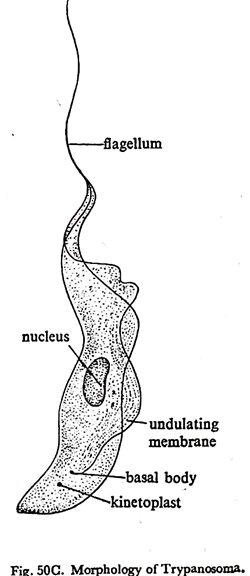
\includegraphics[width=0.5\columnwidth]{A.imagenes/ACV-BioSan-Parasit-TbruceiMorf2}}
	\subfigure[Morfología del tripomastigote.]{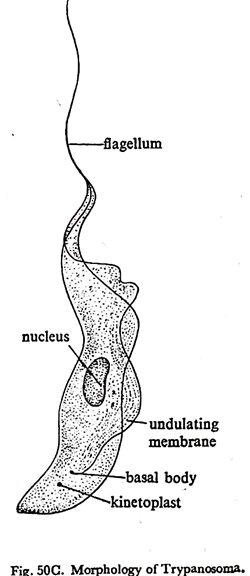
\includegraphics[trim=0 1cm 0 0,scale=0.55,clip]{A.imagenes/ACV-BioSan-Parasit-TbruceiMorf2}}
	\caption[Morfología de \textit{T. brucei}]{Distintas formas parasitarias y ciclo de la morfología de \textit{T. brucei} y detalle de la constitución del tipomastigote sanguineo.\label{fig:PARASIT:TBruceiMorf}}
\end{figure}
\subsubsection{Ciclo biológico}
El ciclo biológico del parásito comienza cuando una mosca tse-tsé sana pica a un animal infectado, con tripomastigotes en sangre. Estos ingresan en el  tracto digestivo de la mosca, dándose una multiplicación por fisión binaria longitudinal. Cuando se verifica, se obtienen, ya en la zona media del intestino, tripomastigotes intestinales. Estos atraviesan la membrana peritrópica, por el espacio endoperitrópico, buscando las glándulas salivales de la mosca. En ellas se da una multiplicación, saliendo, por fisión binaria, dos epimastigotes de cada tripomastigote. Tras ello, ocurre otra multiplicación, formándose tripomastigotes metacíclicos, la forma infectiva para el hospedador vertebrado. Así, cuando la mosca se alimenta de otro hospedador vertebrado, con la saliva viajan los tripomastigotes metacíclicos.

En la picadura, el parásito tiene dos posibilidades: a) pasa directamente a sangre en forma de tripomastigote; o b) se da una multiplicación en los tejidos anejos a la picadura de forma masiva, transformándose en epimastigotes y generándose por ello el chancro tripanosómico. Dentro de ese chancro tripanosómico se encuentran formas esferomastigote y amastigote. Estas se transforman en tripomastigote y pasan a sangre, llegando a otros órganos y multiplicándose en ellos. Cuando una mosca sana chupa la sangre a este hospedador, se lleva tripomastigotes que le infectan, reiniciándose el ciclo.

El tiempo de desarrollo en la mosca es de 3 semanas, mientras que el ser humano es de entre 5 y 12 días, sirviendo de portador. En el tripomastigote metacíclico se forman gran variedad de antígenos, preparándose para ser infectantes. Esta es una forma de evitar que el sistema inmune emita una respuesta que elimine el parásito (gran variabilidad antigénica que evite una respuesta inmune eficaz). Además, el parásito ha creado distintas maneras para perdurar en el tiempo. En el hospedador vertebrado, se dan dos formas de tripomastigote en sangre: las cortas y las largas. Las formas cortas son las infectantes para la mosca y se dan en  momentos en los que baja el número por una respuesta inmune eficaz, asegurándose que pasa a la otra fase del ciclo. Las formas largas se dan cuando hay gran cantidad de estos parásitos.
\begin{figure}[H]
	\centering
	%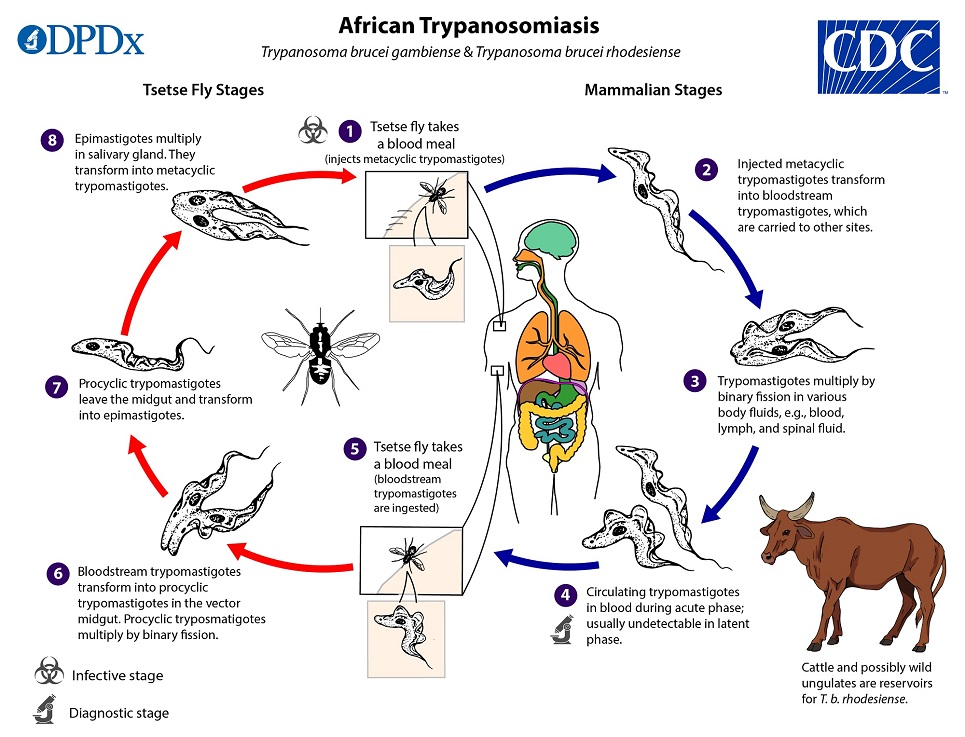
\includegraphics[width=0.8\columnwidth]{A.imagenes/ACV-BioSan-Parasit-TbruceiCBios}
	\caption[Ciclo vital de \textit{T. brucei}]{Ciclo vital de \textit{T. brucei}. Vector: mosca del género \textit{Gossina}. Vía: parenteral. Agente: tripomastigote metacíclico.\label{fig:PARASIT:TBruceiCBios}}
\end{figure}
\subsubsection{Transmisión y control}
Las principales formas de transmisión del parásito son las picaduras del vector (la mosca tsé-tsé) y transfusiones de sangre y trasplantes de órganos. Así, los principales puntos de control son el control del vector mediante insecticidas, repelentes y mosquiteras; diagnóstico y tratamiento de los infectados (control de los reservorios) y control en las transfusiones de sangre y trasplantes de órganos.
\subsubsection{Patología}
De las especies que pueden provocar la enfermedad del sueño, ambas dos provocan la enfermedad con una duración distinta: \textit{T gambiense} cursa de forma crónica (varios meses o años), y \textit{T rhodesiense} cursa de forma aguda (unas semanas a 9 meses). En ambos es común el tiempo de incubación (de 1 a 21 días se puede hallar en sangre), el periodo prepatente (de 7 a 21 días) y el periodo patente (de meses a años). Así mismo, también es común la sintomatología de la enfermedad, que se divide en tres periodos:
\begin{enumerate}[itemsep=0pt,parsep=0pt,topsep=0pt,partopsep=0pt]
	\item \textbf{Periodo inicial} (o de <<incubación>>): dura entre 6 a 14 días, hasta que el parásito llega a sangre. En este periodo se distinguen dos fases:
	\begin{itemize}[itemsep=0pt,parsep=0pt,topsep=0pt,partopsep=0pt]
		\item De 2 a 3 días tras la infección, se forma, en el lugar de la picadura, el chancro tripanosómico: un edema localizado, de centro vesiculoso, bordes descamados y doloroso al tacto. En ese chancro se dan las primeras multiplicaciones del parásito.
		\item De 5 a 12 días tras la infección, se da la parasitemia (elevada si es T rhodesiense) con una fiebre alternante semanal (provocada por picos de parásitos en sangre, hasta que se activa la respuesta inmune, se acompaña de síntomas inespecíficos (periodo prodrómico: malestar general, dolor de cabeza y articulaciones,…)) y anemia normocrónica (por la adsorción de antígenos solubles a eritrocitos sanos, produciendo su lisis por: eritrofagocitosis, activación del complemento o producción de una hemolisina)
	\end{itemize}
	\item \textbf{Periodo segundo}: se pueden encontrar parásitos en linfa, lo que genera una inflamación de los ganglios (sobre todo cervicales) conocidos como signo de Winterbottom, tras 7 a 12 días de la infección. Tras varias multiplicaciones en los ganglios, se da una adenopatía generalizada. En este periodo el parásito llega a distintos órganos: corazón (cardiomegalia, pancarditis), pulmón (edema, congestión por fallo cardiaco).
	\item \textbf{Tercer periodo}: se da la llegada al cerebro del parásito, afectando gravemente al SNC: cefalea intensa, rigidez del cuello, apatía, falta de interés por el trabajo, insomnio, somnolencia, cambio de personalidad, desintegración de funciones del SNC, convulsiones, ataxia, meningitis, y muerte por coma, insuficiencia cardiaca o neumonía.
\end{enumerate}
\subsubsection{Diagnóstico}
\begin{itemize}[itemsep=0pt,parsep=0pt,topsep=0pt,partopsep=0pt]
	\item \textbf{Diagnóstico clínico}: basado en la presencia del chancro tripanosómico, el signo de Winterbottom y fiebre alternante semanal.
	\item \textbf{Diagnóstico etiológico}: búsqueda de tripanosomas en:
	\begin{itemize}[itemsep=0pt,parsep=0pt,topsep=0pt,partopsep=0pt]
		\item \textbf{Chancro}: se hallan formas amastigote y esferomastigote.
		\item \textbf{Sangre}: se hallan tripomastigotes excepto a los 12 días posteriores a la infección; 2 ó 3 días posteriores a la parasitemia y al final de la enfermedad.
		\item \textbf{Linfa}: se encuentran tripomastigotes.
	\end{itemize}
	\item \textbf{Diagnóstico serológico o indirecto}: mediante HAI, ELISA, IFI o F.C.
\end{itemize}
\newpage
\subsection{\textit{Trypanosoma cruzi}}
La enfermedad de Chagas, enfermedad así llamada por el descubridor de su agente etiológico, Carlos Chagas, está causada por el protozoo flagelado \textit{Trypanosoma cruzi}. Descrito en 1909, y llamado así por Oswaldo Cruz, no fue hasta 1930 cuando se le relacionó directamente con el mal de Chagas.

Su distribución se asocia con la de su vector, la vinchuca, chinche asesina o chinche besucona. Esta es la parte continental del mar Caribe, costa pacífica de Méjico, Ecuador, Bolivia, norte y centro de Chile y Argentina y costa atlántica de Brasil (a excepción de la desembocadura del Amazonas). De 120 millones de personas expuestas, entre 16 y 18 millones están parasitadas. Por el mal de Chagas hay unas 50000 muertes anuales en estas zonas, siendo el responsable de la muerte del 30\% de los adultos en Brasil. En Argentina parasita a 3 millones de personas; en EEUU, a 300000; y en España, hasta a unos 68000.
\subsubsection{Morfología}
\begin{multicols}{2}
	\textit{Trypanosoma cruzi} presenta polimorfismo y pleomorfismo. En cuanto a su polimorfismo, se dan varias fases tanto en el hospedador invertebrado como en el cordado, siendo:
	\begin{itemize}[itemsep=0pt,parsep=0pt,topsep=0pt,partopsep=0pt]
		\item \textbf{Hospedador invertebrado}: según avanza en su intestino se dan formas esferomastigote (tracto digestivo inicial), epimastigote (intestino medio) y tripomastigote metacíclico (final del intestino). 
		\item \textbf{Hospedador vertebrado}: en él se dan las formas de amastigote (chagoma), tripomastigote (en sangre) y formas intracelulares intermedias (en células parasitadas, amastigotes).
	\end{itemize}
	\columnbreak
	\begin{figure}[H]
		\centering
		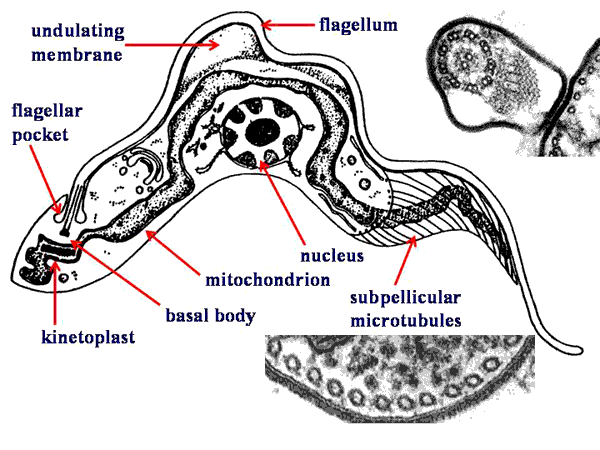
\includegraphics[width=0.8\columnwidth]{A.imagenes/ACV-BioSan-Parasit-TcruziMorf2}
		\caption[Morfología de \textit{T. cruzi}]{Morfología de \textit{T. cruzi}, tripomastigote en sangre. Detalles de los microtúbulos del flagelo. \label{fig:PARASIT:TCruziMorf}}
	\end{figure}
\end{multicols}

Con respecto a formas pleomórficas, se dan las siguientes:
\begin{itemize}[itemsep=0pt,parsep=0pt,topsep=0pt,partopsep=0pt]
	\item En las formas de \textbf{tripomastigote} (sangre del hospedador vertebrado), existen tres formas: cortas, intermedias y largas. Son formas más flexuosas que otros tripanosomas.
	\item En la fase de \textbf{epimastigote} en el intestino medio del vector, existen dos formas: medias y largas.
\end{itemize}
\subsubsection{Ciclo biológico}
\textit{T. cruzi} tiene un ciclo vital que se desarrolla entre dos hospedadores: la vinchuca, un artrópodo de la familia \textit{Reduvidae}, subfamilia \textit{Triatominae}, perteneciente a los géneros: \textit{Triatoma}, \textit{Pastrongylus}, \textit{Rhodnius}; y un mamífero: armadillo, roedores, marsupiales, perros, gatos, humanos,\dots en ninguno de los do hay reproducción sexual, solo se dan multiplicaciones por fisión binaria.

El ciclo comienza con la picadura de una vinchuca parasitada durante la noche (atraída por el CO$_2$ que expele su víctima), normalmente cerca del ojo o los labios. Tras ello, defeca, dejando junto a la herida heces con tripomastigotes metacíclicos. Al rascarse, se introducen en la herida, o cualquier otro punto de entrada (córnea, mucosas,\dots) dándose allí la primera multiplicación. En la piel, cambian de forma al introducirse en las células, transformándose en amastigotes. Una vez se han dado muchas fisiones binarias, el pseudoquiste estalla y libera los amastigotes, que cambian de forma a tripomastigotes en sangre. Estos viajan por el organismo, infectando a otras células (preferentemente a la musculatura no voluntaria). Una vez contactan con una célula, cambian su forma a amastigote, multiplicándose en su interior. Repetirán el ciclo indefinidamente.

El mecanismo de entrada de los tripomastigotes en la célula es sencillo. El parásito se deja fagocitar por la célula objetivo, quedando incluido en una vacuola parasitaria. La célula, mediante la fusión con enzimas líticos, trata de eliminarlo, pero el parásito segrega una enzima, la Tc-Tox, que rompe esas vacuolas, pudiendo darse la multiplicación.

El ciclo biológico termina cuando el hospedador vertebrado es picado de nuevo por una chinche sana, llevándose con la sangre las formas tripomastigote. Estos avanzan por el tracto digestivo y, en el estómago, se transforman en epimastigote, tras lo cual se multiplican, y siguen viajando hasta el fin el intestino del vector, donde se multiplican y se transforman en tripomastigotes metaciclicos, que saldrán de nuevo por las heces.

El tiempo de desarrollo en el vertebrado es de entre 4 a 5 semanas hasta encontrar formas infectantes. En la vinchuca, es de 10 a 8 días.
\begin{figure}[H]
	\centering
	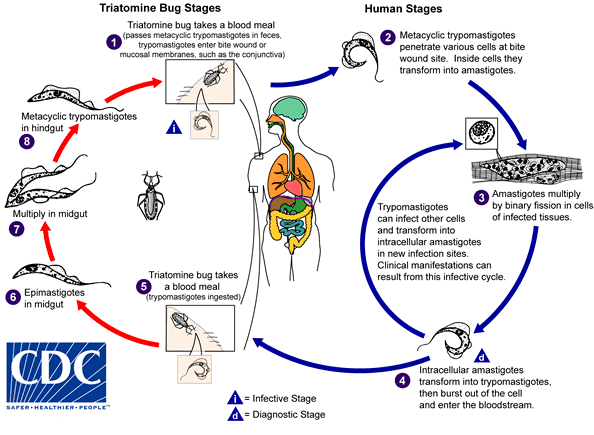
\includegraphics[width=0.7\columnwidth]{A.imagenes/ACV-BioSan-Parasit-TcruziCBios}
	\caption[Ciclo vital de \textit{T. cruzi}]{Ciclo vital de \textit{T. cruzi}. Vector: artŕopodo de la subfamilia \textit{Triatominae}. Vía: parenteral. Agente: tripomastigote metacíclico.\label{fig:PARASIT:TCruziCBios}}
\end{figure}
\subsubsection{Transmisión y control}
Los modos de transmisión más comunes son:
\begin{enumerate}[itemsep=0pt,parsep=0pt,topsep=0pt,partopsep=0pt]
	\item Contaminación de mucosas o heridas por heces de un vector que contengan tripomastigotes metacíclicos.
	\item Transfusiones de sangre y trasplantes de órganos.
	\item Transplacentaria o durante la lactancia
	\item Material quirúrgico o de tatuador contaminado con heces de este parásito.
	\item Contaminación por ingesta de alimentos contaminados con heces contaminadas con tripomastigotes.
\end{enumerate}
Así, las medidas de control son:
\begin{enumerate}[itemsep=0pt,parsep=0pt,topsep=0pt,partopsep=0pt] 
	\item Evitar la picadura de la chinche. Para ello, se invierte en educación sanitaria y en eliminar a la vinchuca del ambiente doméstico y peridoméstico, mediante fumigación, pinturas con insecticidas, barreras físicas (mosquiteras) y alejando a reservorios (otros animales) de ese entorno.
	\item Control en sangre y órganos de la presencia del parásito.
	\item Diagnóstico en embarazos.
	\item Esterilización de material contaminado.
	\item Higiene alimentaria.
\end{enumerate}

La existencia de reservorios mantiene el problema, por ello se hace tan importante el asilar a animales susceptibles de ser reservorios del entorno peridoméstico.
\subsubsection{Patogenia}
La tripanosomosis americana, la enfermedad de Chagas o el mal silenciosos es una enfermedad causada por T. cruzi. Este parásito lleva, sobre todo, una acción traumática de destrucción de las células (cuando una célula del hospedador se infecta, se le denomina pseudoquiste) por masiva multiplicación del parásito en su interior.

El periodo de incubación de la enfermedad es de unos 5 a 20 días, siendo el periodo prepatente de 1 a 2 meses; y el periodo patente de hasta 20 años.

En cuanto a la sintomatología del mal de Chagas, se distinguen cuatro etapas:
\begin{enumerate}[itemsep=0pt,parsep=0pt,topsep=0pt,partopsep=0pt] 
	\item \textbf{Fase inicial} (o de incubación): se puede observar el chagoma (zona enrojecida, eritematosa, de tacto duro y doloroso junto al lugar de la picadura del parásito); linfadenitits (inflamación de los ganglios cercanos al lugar de la infección) y el signo de Romaña (edema de párpado y conjuntiva).
	\item \textbf{Fase aguda}: se da la aparición de la parasitemia y la diseminación de a otros tejidos 60 días después a la infección, apareciendo por ello fiebre alta, dolores musculares o inespecíficos, malestar general (por la multiplicación del parásito en el medio intracelular). Aparecen lesiones en distintos órganos: hepatomegalia, cardiomegalia, miocarditis (provoca taquicardias que, si no son tratadas, llevan a la muerte) y daños en el SNC (aneurismas, irritabilidad y embotellamiento mental (en niños, puede producir un coma que puede llevar a la muerte))
	\item \textbf{Fase latente}: en esta fase, asintomática, el parásito continúa multiplicándose en el interior de las células, pero no genera signos ni síntomas.
	\item \textbf{Fase crónica}: aparece a los 10 o 20 años de la infección. Afecta a ganglios del sistema parasimpático en esófago y colon (10\% de los casos), y provoca distensiones de esófago y colon (megaesófago (regurgitación) y megacolon (estreñimiento), respectivamente) irreversibles.
\end{enumerate}
\subsubsection{Diagnosis}
\begin{itemize}[itemsep=0pt,parsep=0pt,topsep=0pt,partopsep=0pt] 
	\item \textbf{Diagnóstico clínico}: basado en el chagoma y el signo de Romaña.
	\item \textbf{Diagnóstico etiológico}: se puede realizar en:
	\begin{itemize}[itemsep=0pt,parsep=0pt,topsep=0pt,partopsep=0pt] 
		\item Recogida de muestras en el chagoma (macrófagos o histocitos con amastigotes en su interior)
		\item En ganglios inflamados cercanos al lugar de la infección (con tripomastigotes en su interior)
		\item En periodos de fiebre, se hallan tripomastigotes en sangre.
		\item \textbf{Cultivo} de muestras en medio NNN (en caso de poco número, para aumentar su concentración).
		\item \textbf{Xenodiagnóstico}: dejar picar a una chinche sana a un individuo sospechoso y, tras esperar entre 10 y 30 días, buscar en su intestino las diversas formas del parásito.
	\end{itemize}
	\item \textbf{Diagnóstico indirecto}: mediante IFI, ELISA y PCR (reacciones cruzadas con \textit{Leishmania}). Análisis de proteínas por espectrometría (proteómica, 99\% de especificidad).
\end{itemize}
\newpage
\section{Otros Flagelados}
\subsection{\textit{Leishmania} spp}
La leishmaniosis está causada por distintas especies del género \textit{Leishmania}, que se transmite por medio de un vector, un mosquito del género \textit{Phlebotomus} (Viejo Mundo, también conocido como <<beatilla>>) o \textit{Lutzomyia} (Nuevo Mundo), causando hasta tres tipos de parasitosis: leishmaniosis cutánea, mucocutánea y visceral o kala-azar. Las especies son:
\begin{itemize}[itemsep=0pt,parsep=0pt,topsep=0pt,partopsep=0pt] 
	\item Especies responsables de la \textbf{Leishmaniosis visceral}, transmisor \textit{Phlebotomus}:
	\begin{itemize}[itemsep=0pt,parsep=0pt,topsep=0pt,partopsep=0pt] 
		\item[$ $]	\textit{L. (L.) donovani}
		\item[$ $] \textit{L. (L.) infantum} (en España)
		\item[$ $] \textit{L. (L.) archivaldi}
		\item[$ $] \textit{L. (L.) chagasi} (en América, transmisor \textit{Lutzomyia})
	\end{itemize}
	\item Especies responsables de \textbf{Leishmaniosis cutáneas}:
	\vspace*{-0.5cm}
	\begin{multicols}{2}
		\subitem En el Viejo Mundo\footnote{conocido como \textit{Botón de Oriente}}, transmisor \textit{Phlebotomus}.
		\begin{itemize}[itemsep=0pt,parsep=0pt,topsep=0pt,partopsep=0pt]
			\item[$ $] \textit{L. (L.) tropica}
			\item[$ $] \textit{L. (L.) major}
			\item[$ $] \textit{L. (L.) aethiopica} (cutánea difusa)
			\item[$ $] \textit{L. (L.) infantum} (en España)
		\end{itemize}
		\columnbreak
		\subitem En el Nuevo Mundo: transmisor \textit{Lutzomyia}
		\begin{itemize}[itemsep=0pt,parsep=0pt,topsep=0pt,partopsep=0pt]
			\item[$ $] \textit{L. (L.) mexicana}
			\item[$ $] \textit{L. (L.) amazonensis}
			\item[$ $] \textit{L (L.) enrietti}
			\item[$ $] \textit{L. (L.) venezuelensis}
			\item[$ $] \textit{L. (L.) pifanoi}
		\end{itemize}
	\end{multicols}
	\vspace*{-0.5cm}
	\item Especies responsables de \textbf{Leishmaniosis mucocutánea} (Nuevo Mundo) \textit{Lutzomyia}
	\begin{itemize}[itemsep=0pt,parsep=0pt,topsep=0pt,partopsep=0pt]
		\item[$ $] \textit{L. (V.) braziliensis} (espundia)
		\item[$ $] \textit{L. (V.) guyanensis} (pianbois)
		\item[$ $] \textit{L. (V.) panamensis} (afección nasofaríngea rara)
		\item[$ $] \textit{L (LV) peruviana} (uta)
	\end{itemize}
\end{itemize}

En cuanto a su epidemiología:
\begin{itemize}[itemsep=0pt,parsep=0pt,topsep=0pt,partopsep=0pt] 
	\item \textbf{Prevalencia mundial}: 12 millones parasitados (350 millones expuestos) principalmente en regiones tropicales y subtropicales.
	\item \textbf{Incidencia mundial}: 500.000 nuevos casos al año
	\item \textbf{Incidencia en España}: 100-120 casos anuales.
	\item \textbf{Enfermedad reemergente} en Europa: Brotes en países meridionales de Europa (700 casos autóctonos)
\end{itemize}
\subsubsection{Morfología}
Leishmania pertenece a la familia \textit{Trypanosomatide} teniendo también pleomorfismo y polimorfismo:
\begin{itemize}[itemsep=0pt,parsep=0pt,topsep=0pt,partopsep=0pt] 
	\item \textbf{Polimorfismo}: se da por las diferentes formas presentes en su ciclo vital en los dos hospedadores: amastigote (vertebrados) y promastigote, amastigote, esferomastigote y paramastigote (invertebrados)
	\item \textbf{Pleomorfismo}: sólo se da en formas promastigote del estómago del mosquito, habiendo formas neptomonadidas (más de 12 $\mu$m) y haptomonadidas (menos de 12 $\mu$m).
\end{itemize}

Así mismo, el género \textit{Leishmania} se divide en dos subgéneros, según donde se desarrolle en el aparato digestivo del mosquito:
\begin{itemize}[itemsep=0pt,parsep=0pt,topsep=0pt,partopsep=0pt] 
	\item \textbf{Sección \textit{Suprapylaria}}: son especies del subgénero \textit{Leishmania}. El parasito sólo se desarrolla en la región anterior y media del intestino del vector.
	\item \textbf{Sección \textit{Peripylaria}}: son especies del subgénero \textit{Viannia}. Se desarrolla en la zona anterior, media y posterior del parásito.
\end{itemize}

Independientemente del subgénero y especie, la fase infectante para el vertebrado es la de promastigote, y para el mosquito, la de amastigote.
\begin{figure}[htpb]
	\centering
	\subfigure[Fases y morfología en el hospedador vertebrado y en el vector de las dos formas de \textit{Leishmania} spp. \textbf{N}: Núcleo; \textbf{K}: kinetoplasto; \textbf{F}: Flagelo]{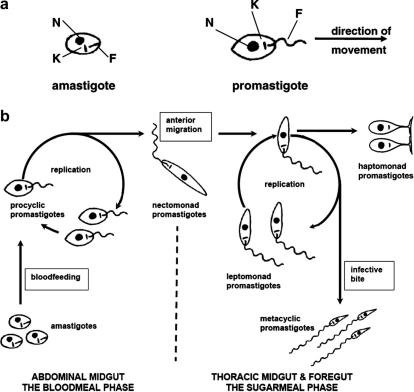
\includegraphics[width=0.475\columnwidth]{A.imagenes/ACV-BioSan-Parasit-LeishmaniaMorf1}}
	\subfigure[Morfología de \textit{Leishmania} (concretamente \textit{L. donovani}) de su vista al microscopio electrónico del tripomastigote en vertebrados]{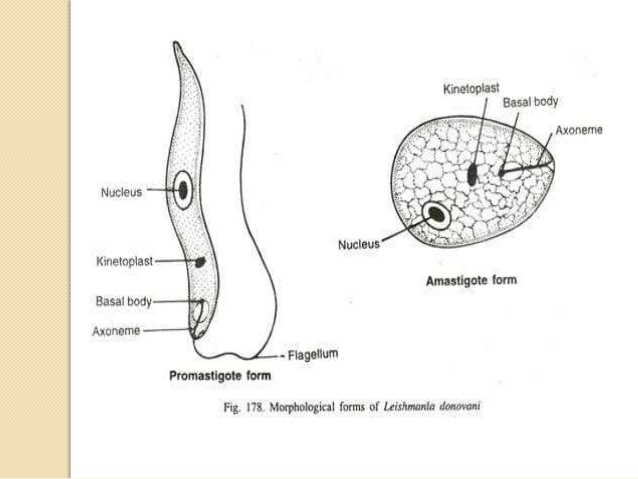
\includegraphics[trim=3cm 3cm 0 0,clip,width=0.475\columnwidth]{A.imagenes/ACV-BioSan-Parasit-LeishmaniaMorf2}}
	\caption[Morfología de \textit{Leishmania}]{Morfología de \textit{Leishmania}, con descripción de sus partes visibles y de sus ciclos biológicos. \label{fig:PARASIT:LeishmaniaMorf}}
\end{figure}
\subsubsection{Ciclo biológico}
Se trata de un parásito heteroxeno (dos hospedadores: vertebrados (roedores, cánidos, carnívoros, caballos y humanos); e invertebrados (mosquitos)). Existen dos ciclos: el zoonótico, en el que es necesario el mosquito; y el antroponótico, consistente en la transmisión entre seres humanos, bien por mosquitos, bien por jeringuillas. 

El ciclo zoonotico comienza cuando un mosquito infectado pica a un individuo no infectado. En el momento de la picadura, con su saliva, el mosquito inyecta formas promastigote que son fagocitadas por los macrófagos. Sobreviven a las vesículas líticas de los macrófagos gracias a la liberación de la proteasa gp63 que protege de la degradación lisosomal, así como de su cubierta polisacarídica (lipofosfoglicano, LPG). Tras penetrar en la célula, se transforman en amastigotes (en el momento de la secreción de gp63) y comienzan a multiplicarse.
 
Tras muchas multiplicaciones, el macrófago estalla, liberando amastigotes que serán de nuevo fagocitados, continuando la parasitosis. El ciclo continúa con la picadura por parte de un mosquito sano que tras la ingesta, los amastigotes, en su estómago, se multiplican y cambian de conformación a promastigote (formas neptomonadidas en su zona media del estómago y, en la banda estomodal, formas haptomonadidas). En el esófago, se transforman en paramastigotes que al avanzar a la faringe pasan a formas promastigote. En especies de la sección peripilaria también se da multiplicación en el píloro, siendo el resto del ciclo de la misma forma.
\begin{figure}[H]
	\centering
	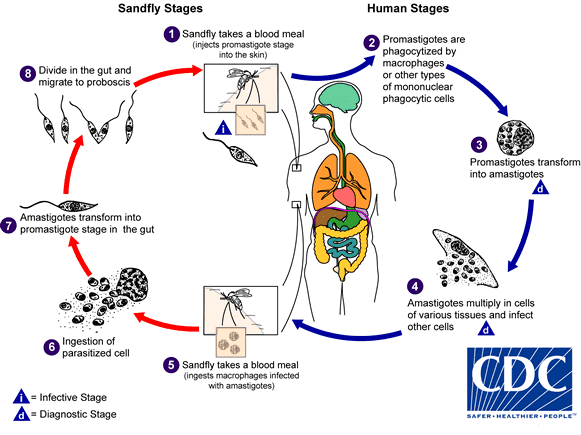
\includegraphics[width=0.75\columnwidth]{A.imagenes/ACV-BioSan-Parasit-LeishmaniaCBios}
	\caption[Ciclo biológico de \textit{Leishmania} spp]{Ciclo biológico de \textit{Leishmania} spp. Vector: mosquito; Agente: promastigote; Vía: parenteral.}
\end{figure}
\subsubsection{Control}
\begin{itemize}[itemsep=0pt,parsep=0pt,topsep=0pt,partopsep=0pt] 
	\item Evitar la picadura del insecto mediante mosquiteras, repelentes,$\dots$
	\item Control de reservorios y control y tratamiento de los infectados.
	\item No compartir jeringuillas (resulta especialmente incidente en pacientes seropositivos contagiados por el uso compartido de jeringuillas, siendo además oportunista (gran desarrollo de la enfermedad en pacientes con linfocitos CD4$^+$ en niveles menores a 50 udd/mL)).
\end{itemize}
\subsubsection{Vector y epidemiologia}
La leishmaniosis se transmite por la inoculación en la picadura de formas promastigote presentes en la saliva de dos mosquitos: \textit{Phlebotomus} y \textit{Lutzomyia}. Estos mosquitos son capaces de sobrevivir 1 mes infectados, siendo transmisores a partir de los 3 o 4 días de la infección. Pican las hembras al atardecer, yendo a zonas oscuras, haciendo vuelos cortos y rastreros en días sin viento. Tienen piezas bucales cortas, pudiendo picar solo en zonas de piel desnuda. Los reservorios de la enfermedad son carnívoros y mamíferos medianos.

Estos mosquitos se diferencian por:
\begin{table}[H]
	\centering
	\begin{tabular}{cc}
		\rowcolor{black}\textcolor{white}{\textit{\textbf{Phlebotomus}}}&\textcolor{white}{\textit{\textbf{Lutzomyia}}}\\
		Propios del Viejo Mundo&Propios del Nuevo Mundo\\
		(Mediterráneo, Próximo Oriente, India, África Tropical)&Zonas tropicales.\\
		\rowcolor{hiperlightgray}Regiones semiáridas (grietas, huecos en árboles, suelo)&Zonas boscosas (selva)\\
		Necesitan humedad pero no corrientes de agua&Precisan de un alto grado de humedad\\
		\hline
	\end{tabular}
	\caption{Comparativa entre los diferente vectores de \textit{Leishmania}.}
\end{table}
\subsubsection{Patología y sintomatología}
Se diferencian tres tipos de leishmaniosis, causadas por las citadas especies del género \textit{Leishmania}.
\paragraph{Cutánea}
Es la única de las leishmaniosis que es capaz de producir una cierta inmunidad. Su periodo de incubación es muy variable: de días a años. En el punto de la picadura del mosquito, el punto de la infección, se forma una pápula roja que, a los pocos días, se forma una costra y, tras ella, se ulcera (la parasitosis puede complicarse debido a otras infecciones secundarias que aprovechen la úlcera para introducirse en el organismo). La úlcera se cierra, se da la curación espontánea, siendo así efectiva la gran respuesta inmune, en un plazo de dos meses a un año, dejando una cicatriz despigmentada.

Esta enfermedad la provocan dos especies distintas, \textit{L. tropica} y \textit{L. major}, con dos comportamientos ciertamente distintos:
\begin{table}[H]
	\centering
	\begin{tabular}{cc}
		\rowcolor{black}\textcolor{white}{\textit{\textbf{Leishmania tropica}}}&\textcolor{white}{\textit{\textbf{Leishmania major}}}\\
		Se da en zonas urbanas muy pobladas. Sin reservorios.&Zonas rurales poco habitadas.\\
		&Con reservorios (animales domésticos).\\
		\rowcolor{hiperlightgray}Pápula seca, roja y con muchos amastigotes en ella.&Pápula húmeda, roja, bulbosa y con pocos\\
		\rowcolor{hiperlightgray} Persiste meses sin ulcerar.& amastigotes en ella. Se ulcera con facilidad.\\
		Su curación sólo da inmunidad frente a \textit{L. tropica}.&Produce inmunidad frente a\textit{ L. tropica} y \textit{L. major}\\
		\hline
	\end{tabular}
	\caption{Leishmaniosis cutánea: principales agentes y comparación}
\end{table}

Otro tipo de leishmaniosis cutáneas son:
\begin{itemize}[itemsep=0pt,parsep=0pt,topsep=0pt,partopsep=0pt]
	\item \textbf{Leishmaniosis cutánea difusa}: provocada por \textit{L. aethiopica} y \textit{L. pifani}. Se trata de una leishmaniosis parecida a la cutánea en la que las úlceras se difunden por todo el tegumento.
	\item\textbf{Úlcera del chiclero}: causada por \textit{L. mexicana}. El mosquito (genero \textit{Lutzomyia}) que vive en el árbol del chicle (en sus hojas y en la corteza) pica sobre todo en la oreja, donde degrada la piel y el cartílago de zonas anexas a la picadura.
\end{itemize}
\paragraph{Mucocutánea}
La especie tipo de esta parasitosis es \textit{Leishmania Viannia braziliensis}. El 90\% de los casos de esta enfermedad se hallan entre Bolivia, Brasil y Perú. La picadura del mosquito da lugar a una lesión en la piel parecida a la de la leishmaniosis cutánea: formación de una pápula roja a la que siguen lesiones secundarias por infección de ésta. Cuando se cura, comienzan a verse daños en mucosas de otras partes del cuerpo: se forman pápulas que acaban por ulcerarse y son especialmente predispuestas a infectarse, generando infecciones secundarias que acaban por llevar a la muerte si no hay tratamiento. La formación de úlceras se relaciona con metástasis en tabique nasal y faringe, pudiendo además destruir partes blandas de nariz, paladar o labios.
\paragraph{Visceral o Kala-azar}
Esta leishmaniosis es muy prevalente en la zona de la India y África. El periodo de incubación de esta enfermedad es muy variable (de 10 días a un año). Primeramente aparece una lesión cutánea que pasa desapercibida (pequeña pápula) y donde se da la primera multiplicación. A partir de ahí, pasa a sangre, llegando a hígado y bazo, donde se multiplicará en el interior de los macrófagos de estos órganos.
La multiplicación del parásito se asocia a una disminución de células sanguíneas (anemia normocítica, leucopenia y trombocitopenia) lo que genera una hiperplasia de hígado y bazo en su función de más elementos formes sanguíneos (hepatomegalia, esplenomegalia) y un incremento inespecífico de las inmunoglobulinas y un descenso de la albúmina.

La sintomatología de la enfermedad se desarrolla de la siguiente forma: aparece una fiebre inicial, vómitos y un agotamiento progresivo. Pueden aparecer pigmentaciones oscuras en la piel, lo que se ha llamado fiebre negra. Se produce una distensión abdominal y aparecen dolores en el abdomen acompañados, al final de la enfermedad, de disenterías. Sin tratamiento provoca la muerte en 2 ó 3 años. Las manifestaciones más agudas cursan con fiebre, frío, vómitos, edemas, hemorragias en las mucosas, dificultad respiratoria y muerte entre los 6 y 12 meses posteriores a la infección. 
\subsubsection{Diagnóstico}
\begin{itemize}[itemsep=0pt,parsep=0pt,topsep=0pt,partopsep=0pt] 
	\item \textbf{Mucocutánea y cutánea}
	\begin{itemize}[itemsep=0pt,parsep=0pt,topsep=0pt,partopsep=0pt] 
		\item \textbf{Clínico}: se puede identificar inequívocamente por las lesiones generadas en la piel.
		\item \textbf{Etiológico}: se puede optar mediante el visionado directo de muestras de piel de pápulas (se observan macrófagos con Leishmania en su interior), o, si no hay gran cantidad de parásitos, concentrarlo mediante cultivo en NNN o RPMI y agar sangre. También existe la posibilidad del xenodiagnóstico, ya sea por inoculación a un mosquito sano y su posterior disección, o inoculándosela a un ratón.
		\item \textbf{Inmunodiagnóstico}: pueden hacerse pruebas inmunohistoquímicas que identifiquen  al parasito dentro de las células; ELISA, IFI o Western Blot, aunque existen reacciones cruzadas con \textit{Trypanosoma} spp, \textit{Mycobacterium leprae} y \textit{Mycobacterium tuberculosis}; y por último, la intradermorreacción de Montenegro (inyección de antígenos de Leishmania y ver si existe un eritema (positivo si es mayor de 5 mm.). La prueba tiene una sensibilidad del 95\%, pero una vez hecha, provoca una inmunidad en el paciente que genera falsos positivos al repetirla.
		\item \textbf{PCR}: resulta especialmente útil para identificar la especie causante.
	\end{itemize}
	\item \textbf{Visceral}: Dado que la pápula no es llamativa y los otros síntomas pueden llevar a confusión, no existe diagnóstico clínico.
	\begin{itemize}[itemsep=0pt,parsep=0pt,topsep=0pt,partopsep=0pt] 
		\item \textbf{Etiológico}: Leishmania no se puede encontrar en frotis sanguíneos, recurriéndose a punciones de médula ósea, hepática y bazo. Estas muestras recogidas se pueden concentrar mediante cultivo en RPMI o NNN; o se puede realizar xenodiagnóstico (inocularle el aislado a animales de experimentación). 
		\item \textbf{Indirecto}: Se puede hacer mediante IFI o ELISA. No tiene valor la prueba de Intradermorreacción de Montenegro. 
		Otra prueba específica para el kala-azar o leishmaniosis visceral es la reacción de formol-leuco-gelificación, que permite detectar la gran elevación de anticuerpos asociados a esta enfermedad. El mecanismo es el siguiente: se toman unas 20 gotas de suero problema al que se le
	\end{itemize} añaden 2 gotas de formol al 40\%. Se espera 30 minutos y se observa: si se gelifica, la reacción es positiva; si permanece líquido, la reacción es negativa.
\end{itemize}
\newpage
\subsection{\textit{Giardia lambia}}
La giardiosis es una enfermedades transmitidas por parásitos protozoarios intestinales relativamente comunes y de amplia distribución mundial. De ciclos y sintomatología parecida \textit{Balantidium coli}, son relativamente distantes en cuanto a su taxonomía.
\subsubsection{Morfología}
\textit{Giardia lamblia} es un flagelado anaerobio intestinal de distribución cosmopolita, pero de mayor incidencia en zonas cálidas y templadas. Carece de mitocondrias y aparato de Golgi, se reproducen por fisión binaria longitudinal. Posee dos formas:
\begin{itemize}[itemsep=0pt,parsep=0pt,topsep=0pt,partopsep=0pt]
	\item \textbf{Trofozoito}: con dos núcleos, piriformes (en forma de careta, siendo los núcleos los ojos), posee simetría longitudinal. Tiene 4 pares de flagelos a cada lado: un par anterolateral, un par ventral, un par posterolateral y un par caudal. Estos últimos nacen en la parte anterior (en la parte redondeada), recorriendo el axonema todo el citoplasma, rígidos, formando el funis. Los núcleos se sitúan a ambos lados del funis, teniendo grandes nucléolos. Presentan también dos cuerpos medios curvos. En su citoplasma hay gran cantidad de ribosomas, RE y gránulos de glucógeno. La parte redondeada recibe el nombre de disco suctor, estructura con la que se adhiere a las vellosidades intestinales.
	\item \textbf{Quiste}: son ovalados, con 2 (inmaduros) o 4 (maduros) núcleos. Tiene restos de axonemas y de los cuerpos medios. Presentan un citoplasma muy colapsado.
\end{itemize}
\subsubsection{Ciclo biológico}
Se trata de un ciclo biológico directo monoxeno, teniendo varios reservorios (perros, gatos, ganado, primates). Una vez entran los quistes de Giardia lamblia en el organismo (por vía oral, vehiculizado por alimentos o agua contaminados por quistes (de 2 o 4 núcleos (inmaduros y maduros, respectivamente)). Al llegar al duodeno, eclosionan, obteniéndose 1 ó 2 trofozoitos, que continúan dividiéndose a lo largo que viajan por el intestino. Al llegar al colon, la falta de humedad hace que comience la fase de enquistación, que, ya sean maduros o inmaduros, salen al exterior por las heces, siendo capaces de poder reiniciar el ciclo.

Las moscas pueden actuar como transmisiones mecánicos de los quistes.
\begin{multicols}{2}
	\begin{figure}[H]
		\centering
		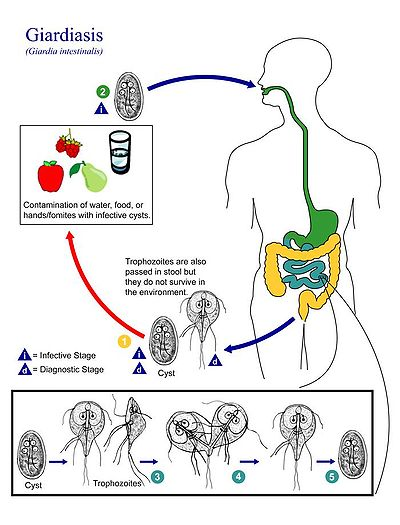
\includegraphics[width=0.895\columnwidth]{A.imagenes/ACV-BioSan-Parasit-GlambiaCBios}
		\caption[Ciclo biológico de \textit{G. lambia}]{Ciclo biológicos de \textit{G. lambia}. Vehículo: comida y agua infectadas, Vía: oral, Agente: Quiste.\label{fig:PARASIT:GLambiaCBios}}
	\end{figure}
	\columnbreak
	\begin{figure}[H]
		\centering
		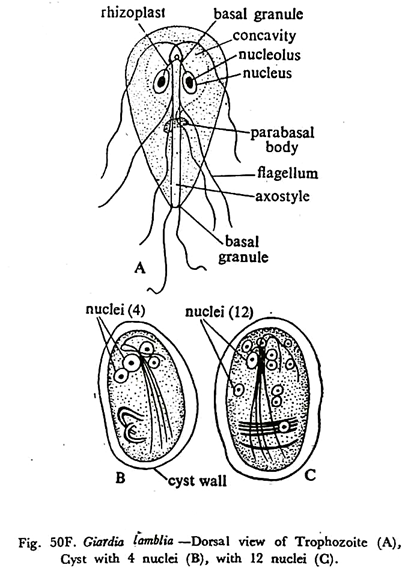
\includegraphics[trim= 0 1cm 0 0,clip,width=0.9\columnwidth]{A.imagenes/ACV-BioSan-Parasit-GlambiaMorf}
		\caption[Morfología de \textit{G. lambia}]{Morfología de \textit{G. lambia}. En la parte superior (\textbf{A}), la forma parasitaria; en la parte inferior, la forma de resistencia e infecciosa, el quiste, con (\textbf{B}) 4 núcleos y con (\textbf{C}) 8 núcleos.\label{fig:PARASIT:GLambiaMorf}}
	\end{figure}
\end{multicols}
\subsubsection{Epidemiología}
Presenta prevalencias variables (un 2\% en adultos y un 7\% de niños en países desarrollados, frente a un 33\% en países en desarrollo). Es la infección protozoaria más común en el ser humano, con una prevalencia de 280 millones de personas, y una incidencia de 500000 casos anuales (600 en España). La dosis infectiva es de entre 10 y 100 quistes, pero un individuo parasitado llega a arrojar hasta 10 billones de estas formas de manera diaria. La principal población de riesgo son los niños, personal de guarderías, turistas, ganaderos y homosexuales (contacto oral-anal).

Las principales medidas de control son el lavado adecuado de alimentos (3 gotas de Na(ClO) por litro de agua, durante 10 minutos) y de manos, para evitar la transmisión. Así mismo, el control de aguas, la correcta manipulación de alimentos y la higiene personal y comunitaria.
\subsubsection{Patogenia y sintomatología}
\textit{Giardia lamblia} tiene un tiempo de incubación de entre 7 y 20 días, un periodo patente desde horas hasta un par de días, y un periodo patente de meses o años. No presentan acción patógena traumática (no invaden las mucosas), siendo su acción patógena la deformación (aplanamiento) de las vellosidades intestinales.

Esta acción genera irritación en el intestino, que causa casi todos los síntomas de la enfermedad: nauseas, vómitos, dolor epigástrico sordo o vago, meteorismo, irritación duodenal por exceso de producción de mucus, síndrome de malabsorción (no se absorben las grasas ni vitaminas liposolubles, generando adelgazamiento y pérdida de apetito; y en el caso de niños, retraso mental) fiebre y diarrea (que pueden ser crónicas o agudas (continuas o intermitentes) con esteatorrea (heces grasientas). En algunas ocasiones se puede ver afectada la vesícula biliar (provocando ictericia y cólicos biliares) por acción mecánica obstructiva (impiden el paso de la bilis).
\subsubsection{Diagnosis}
\begin{itemize}[itemsep=0pt,parsep=0pt,topsep=0pt,partopsep=0pt]
	\item \textbf{Clínico}: un síntoma indicativo, pero no excluyente, de giardiosis es la esteatorrea (heces grasientas)
	\item \textbf{Etiológico}: se puede hacer mediante coprología (recogida de heces de tres días distintos y se examinan directamente o mediante técnicas de concentración (Bailenger) y posterior visualización), recogida de muestras por aspirado duodenal (y posterior visualización) o mediante PCR (aplicado a las muestras, permitiendo reconocer subtipos). 
	\item \textbf{Inmunológico}: se basa en la búsqueda y detección de coproantígenos en muestras de heces mediante ELISA, IFD.
\end{itemize}
\newpage
\subsection{\textit{Trichomonas vaginalis}}
De las dos especies del género \textit{Trichomona} que pueden vivir en el cuerpo humano, la única que presenta una importancia clínica es \textit{T. vaginalis}. La otra, \textit{T. hominis}, es un parasito comensal del intestino.

\textit{Trichomonas vaginalis} parasita la vagina y las glándulas prostáticas. Cosmopolita, su incidencia mundial es de 180 millones de casos (200 en España) cada año. La población de riesgo son prostitutas y el 100\% de las compañeras sexuales de varones tricomoniósicos. 
\subsubsection{Morfología}
\textit{Trichomonas vaginalis} no forma quistes. El trofozoito emite pseudópodos y está flagelado. Presenta 4 flagelos libres y uno unido a la membrana plasmática que la curva (recurrente), formando una membrana ondulante. Este último flagelo no sale, frente a T. hominis, que si es libre.

Presenta un núcleo, aparato de Golgi,  y una fibra solo visible al MET, denominada pelta que forma parte de las fibras parabasales. Así mismo, tiene un citostoma solo visible al MET y una gran cantidad de formaciones rígidas con función de soporte. Estas últimas son el axostilo (estructura que viaja desde el polo anterior al posterior, saliendo de la célula) y la costa (estructura cilíndrica y delgada situada bajo la membrana ondulante que la soporta y permite dar la forma). Junto a estas estructuras se encuentran gran cantidad de hidrogenosomas, paracostales y paraaxostilares, según se encuentren al lado de que estructura.

Esta célula se alimenta sobre todo de bacterias de la vagina.
\subsubsection{Ciclo biológico}
El ciclo de \textit{Trichomonas vaginalis} es un ciclo directo y sin reservorios (se dan infecciones de persona a persona). Transmitido por vía venérea, en el parto a recién nacidas y por instrumental ginecológico mal esterilizado. 

Las medidas de control más eficientes son el uso de preservativos y la detección y tratamiento adecuado de hospedadores (sobre todo varones asintomáticos).
\begin{multicols}{2}
	\begin{figure}[H]
		\centering
		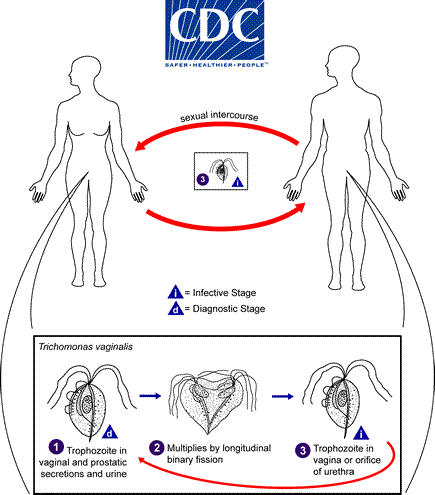
\includegraphics[width=\columnwidth]{A.imagenes/ACV-BioSan-Parasit-TVaginalisCBios}
		\caption[Ciclo biológico de \textit{T. vaginalis}]{Ciclo biológicos de \textit{T. vaginalis}. Vehículo: infección directa, Vía: sexual, Agente: Trofozoito.\label{fig:PARASIT:TvaginalisCBios}}
	\end{figure}
	\columnbreak
	\begin{figure}[H]
		\centering
		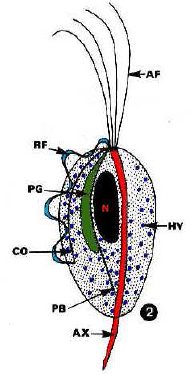
\includegraphics[width=0.585\columnwidth]{A.imagenes/ACV-BioSan-Parasit-TVaginalisMorf}
		\caption[Morfología de \textit{T. vaginalis}]{Morfología de \textit{T. vaginalis}. \textbf{AF}: Flagelos libres; \textbf{RF}: Membrana ondulante (flagelo); \textbf{PG}: Pelta o aparato de Golgi; \textbf{CO}: costa; \textbf{N}: núcleo; \textbf{HY}: citoplasma (hidrogenosomas); \textbf{PB}: fibras parabasales; \textbf{AX}: axostilo.\label{fig:PARASIT:TvaginalisMorf}}
	\end{figure}
\end{multicols}
\subsubsection{Patogenia y sintomatología}
La trichomonosis tiene un periodo de incubación de 4 a 28 días, un periodo prepatente de 4 a 28 días, y un periodo patente de meses o años. La principal acción de Trichomonas vaginalis es una acción traumática en el cérvix, provocando inflamación. Esta inflamación provoca la degeneración del epitelio del cuello de útero, evolucionando la enfermedad de dos maneras distintas:
\begin{itemize}[itemsep=0pt,parsep=0pt,topsep=0pt,partopsep=0pt]
	\item \textbf{Agudo}: se produce un flujo vaginal lechoso, purulento y fétido, siendo prueba patente de la enfermedad.
	\item \textbf{Crónico}: el flujo vaginal no presenta tantos leucocitos como en el curso agudo, pero se halla presente \textit{T. vaginalis} y una gran cantidad de células epiteliales.
\end{itemize}

La erosión del cérvix genera predisposiciones a sufrir carcinoma y es factor de riesgo para la infección de VIH y HVS-2. En varones suele ser asintomática, generando, a veces, prostatitis, uretritis, irritación temporal en el pene, ligero ardor tras orinar o eyacular y, en contados casos, esterilidad (reversible).

La sintomatología solo se presenta en el 30\% de los individuos parasitados. Esta es: escozor, prurito vulvar y vaginal, cambio de aspecto de las secreciones vaginales, vulvitis, dolor en la parte baja del vientre, cistitis y disuria.
\subsubsection{Diagnóstico}
\begin{itemize}[itemsep=0pt,parsep=0pt,topsep=0pt,partopsep=0pt]
	\item \textbf{Etiológico}: observación directa en secreciones vaginales o prostáticas y en sedimentos urinarios (hay que tomar medidas frente a contaminación con heces (falsos positivos por \textit{Trichomonas hominis}), cultivo de muestras en medios con suero y caseína hidrolizada (durante 7 días), o mediante PCR.
	\item \textbf{Indirecto}: mediante aplicaciones de HAI, IFI o ELISA de suero del paciente. Puede cuantificarse la cantidad de parásitos.
\end{itemize}
\newpage
\section{\textit{Apicomplexa}}
Los coccidios son una clado dentro del phylum \textit{Apicomplexa}, concretamente, dentro de la clase \textit{Sporozoea}, subclase \textit{coccidia}. Este clado se caracteriza por poseer todas las características tipo del filum. Esta es la posesión del complejo apical.

El complejo apical está formado por un orificio localizado en un polo de la célula, denominado anillo polar (pudiendo haber  uno o dos), que le corresponde uno en el otro extremo (anillo posterior). Bajo este anillo polar se encuentra el conoide, una formación cónica en espiral en cuyo centro se hallan las rotrias (cuyo número varía según la especie) en cuyo final, y a lo largo del conoide se hallan los micronemas, cuerpos vesiculares con sustancias proteicas en su interior que, en el caso de protozoos intracelulares, poseen sustancias líticas que permiten parasitar a la célula diana. Surgiendo del anillo polar, y cubriendo todo el cuerpo, se hallan los microtúbulos subpediculares. Bajo la estructura citoesquelética del complejo se halla una vacuola vestigial, el apicoplasto.

Así mismo, dentro del filum se dan las siguientes formas de reproducción:
\begin{itemize}[itemsep=0pt,parsep=0pt,topsep=0pt,partopsep=0pt]
	\item \textbf{Fisión binaria} (bipartición): la más frecuente, a partir de una célula madre se forman dos células hijas por previa cariocinesis seguida de una citocinesis. Según el plano de división son: a) anárquicas (amebas, sin plano de división definido); b) longitudinal o simetrogónica (flagelados, sigue una simetría longitudinal); y c) transversal u homotetogónica (ciliados).
	\item \textbf{Esquizogonia asexual}: en este proceso, el núcleo se divide varias veces, formando un ser multinucleado (esquizonte). Cada uno de esos núcleos se rodea de una porción de citoplasma, ocurriendo la división del citoplasma. A cada célula hija se le denomina merozoito.
	\item \textbf{Esporogonia}: se trata de una fisión múltiple tras una reproducción sexual (unión de gametos. Tras la formación del zigoto, se produce una meiosis y luego repetidas meiosis. Así, del ooquiste (con el cigoto en su interior), se forma, por meiosis, dos esporoblastos que, tras una mitosis, forma dos esporoquistes, con sendos dos o más esporozoitos en su interior.
	\item \textbf{Singamia} o \textbf{reproducción sexual}: proceso de unión de gametos y fusión de núcleos para formar, en el caso de los protozoos, un cigoto diplonte. Puede ser: isogamica (los gametos son iguales) o anisogámica (gametos distintos). El primer paso, en ambos casos, es la gamogonia o gametogénesis (proceso de formación de los gametos), llevado a cabo por los gamontes (células sexuales inmaduras que originan los gametos). En el caso de la anisogamia se diferencian dos gametocitos: el microgametocito (formado por un microgamonte que se divide muchas veces formando gametos pequeños) y el macrogamtocito (generado a partir de un único macrogamonte).
	\item \textbf{Endopoligenia} y \textbf{endodiogenia}: se trata de divisiones asexuales múltiples y binarias donde se obtienen taquizoitos o bradizoitos, respectivamente. Se diferencian de la esquizogonia en que en este proceso la membrana se forma de novo y no se verifica la división hasta que están perfectamente formadas, produciéndose entonces la rotura de la membrana de la célula madre.
\end{itemize}
\newpage
\subsection{\textit{Cryptosporidium parvum}}
\subsubsection{Morfología}
\textit{Cryptosporidium parvum} es un parásito intestinal de muchos animales y, entre ellos, del ser humano. Protozoo no flagelado, es cosmopolita y eurixeno. La incidencia en España es de unos 100 a 200 casos anuales. Está considerada una enfermedad emergente (se creía que solo afectaba a ratones, pero casos de inmunodepresión permitieron su localización en humanos) y ocupacional (es frecuente en personas en contacto directo con excretas animales). La población más expuesta a esta enfermedad son los individuos inmunosuprimidos, dado que las diarreas que causa en ellos no son autolimitantes, complicándose la enfermedad. Presenta dos formas:
\begin{itemize}[itemsep=0pt,parsep=0pt,topsep=0pt,partopsep=0pt]
	\item \textbf{Trofozoito}: tiene forma alargada y pequeña, midiendo hasta 5 $\mu$m, con puntas romas en sus extremos. En su polo apical presenta el complejo apical propio del phylum \textit{Apicomplexa}. Bajo este se halla un pequeño citostoma (microporo). Presenta un núcleo grande con un nucléolo grande. En su citoplasma se halla un aparato de Golgi, un retículo endoplásmico y mitocondrias. Las formas de trofozoito reciben un nombre distinto según se originen de esporogonias, gamogonias,… su localización habitual es el interior del enterocito, entrando en el mediante fagocitosis inducida, disponiéndose bajo el borde en cepillo.
	\item \textbf{Ooquiste}: fase de resistencia, presenta una cubierta externa quística protectora, con un orificio taponado (micropilo), los esporoquistes y una masa de restos de las divisiones celulares, el residuo ooquistico. Una vez maduro, ese micrópilo se abre y deja salir las fases al exterior. En el interior de estos se forman los esporoquistes, unas estructuras cubiertas por una membrana con los esporozoitos en su interior (con su forma de coccidio típica) y un residuo esporoquistico. Forman 4 esporozoitos en su interior, en un solo esporoquiste
\end{itemize}
\subsubsection{Ciclo biológico}
La vía de infección de \textit{Cryptosporidium parvum} es la ingesta de agua o alimentos contaminados con ooquistes maduros. 

Los ooquistes aguantan el pH estomacal, abriéndose en el intestino. Los esporozoitos que surgen del ooquistes se pegan al epitelio intestinal, fijándose, redondeándose y provocando su endocitosis y formación de una vacuola que les engloba en el interior del enterocito. En el interior de la vacuola, por esquizogonia, comienza a multiplicarse, surgiendo hasta merozoitos por esquizonte. Cuando estos merozoitos crecen, hacen estallar a la célula, reiniciando el ciclo infectivo estos merozoitos. Tras varias esquizogonias, se da una gamogonia, siendo anisogámica: en la invasión de los enterocitos, parte de los merozoitos formaran microgametocitos (16 por merozoito) y parte formaran macrogametocitos (1 por merozoito). Los gametocitos se liberan y, si se encuentran, ocurre la fecundación, generando un cigoto que formará un ooquiste, pudiendo seguir dos caminos:
\begin{enumerate}[itemsep=0pt,parsep=0pt,topsep=0pt,partopsep=0pt]
	\item El ooquiste inmaduro se libera al exterior del organismo, ocurriendo ahí su maduración, formando 4 esporozoitos con un residuo ooquistico.
	\item Se da una esporogonia en el interior del hospedador, madurando en el enterocito donde se dio la fecundación, rompiendo la célula y liberándose al exterior.
	\item En personas con problemas de inmunosupresión se da el fenómeno de la endoautoinvasión: antes de ser evacuados, el ooquiste se rompe y reinicia el ciclo esquizogónico.
\end{enumerate}

Así, el principal elemento de control de esta parasitosis es el evitar ingerir ooquistes contaminados (higiene alimentaria) y el control de las excretas.
\subsubsection{Patogenia y sintomatología}
El periodo de incubación de la cryptosporidiosis es de 3 a 12 días, el periodo prepatente es de unos 4 días, siendo el patente de 2 a 4 semanas (en inmunocompetentes, llegando a ser mortal en inmunosuprimidos (endoautoinvasión)).

La acción patógena de este parásito es, principalmente, traumática en células intestinales (provoca la destrucción del epitelio intestinal). La sintomatología de esta enfermedad es, sobre todo, diarreas intensas y acuosas. En inmunosuprimidos, estos protozoos llegan a otras localizaciones extraintestinales: vesícula biliar (colecistitis y colangitis, ictericia), conductos pancreáticos (pancreatitis) o vías respiratorias (tos, ronquera).
\subsubsection{Diagnóstico}
\begin{itemize}[itemsep=0pt,parsep=0pt,topsep=0pt,partopsep=0pt]
	\item \textbf{Etiológico}: mediante coprología, tomando una muestra de heces sospechosas y, una vez aplicada una tinción Ziehl-Nielsen, buscar ooquistes (tinción verde). No se ha de confundir con restos de descamación intestinal ni con otros coccidios intestinales (Cyclospora, Cystoisospora).
	\item \textbf{Técnicas indirectas}: pueden diagnosticarse mediante técnicas de detección de ooquistes en heces por IFI o ELISA.
\end{itemize}
\begin{multicols}{2}
	\begin{figure}[H]
		\centering
		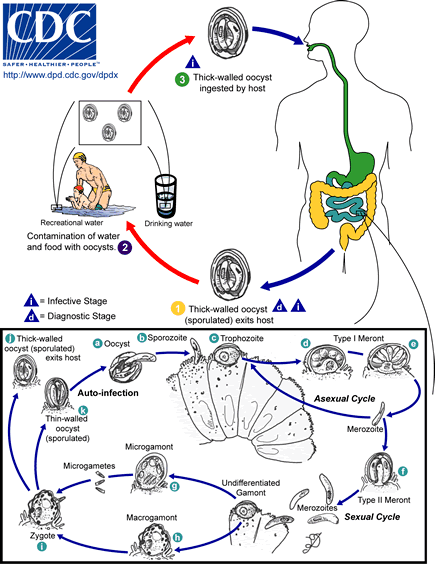
\includegraphics[width=\columnwidth]{A.imagenes/ACV-BioSan-Parasit-CparvumCbios}
		\caption[Ciclo biológico de \textit{C. parvum}]{Ciclo biológicos de \textit{C. parvum}. Vehículo: agua o alimentos contaminados, Vía: oral, Agente: Ooquiste.\label{fig:PARASIT:CparvumCBios}}
	\end{figure}
	\columnbreak
	\vspace*{2.47cm}
	\begin{figure}[H]
		\centering
		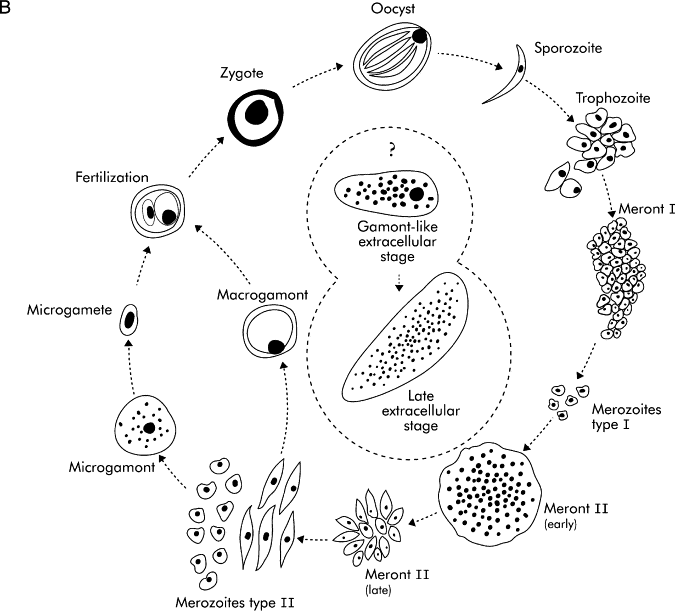
\includegraphics[width=\columnwidth]{A.imagenes/ACV-BioSan-Parasit-CparvumMorf}
		\caption[Morfología de \textit{C. parvum}]{Morfología de \textit{C. parvum} y los distintos estadíos del parásito.\label{fig:PARASIT:CparvumMorf}}
	\end{figure}
\end{multicols}
\newpage
\subsection{\textit{Cystoisospora belli}}
\subsubsection{Morfología}
Enfermedad emergente parasitaria, de distribución cosmopolita y frecuente en zonas tropicales y templadas. 
\begin{itemize}[itemsep=0pt,parsep=0pt,topsep=0pt,partopsep=0pt]
	\item \textbf{Trofozoito}: tiene forma alargada, con puntas romas en sus extremos. En su polo apical presenta el complejo apical propio del phylum \textit{Apicomplexa}. Bajo este se halla un pequeño citostoma (microporo). Presenta un núcleo grande con un nucléolo grande. En su citoplasma se halla un aparato de Golgi, un retículo endoplásmico y mitocondrias. Las formas de trofozoito reciben un nombre distinto según se originen de esporogonias, gamogonias,… su localización habitual es el interior del enterocito, entrando en el mediante fagocitosis inducida, disponiéndose bajo el borde en cepillo.
	\item \textbf{Ooquiste}: fase de resistencia, presenta una cubierta externa quística protectora, con un orificio taponado (micropilo), los esporoquistes y una masa de restos de las divisiones celulares, el residuo ooquistico. Una vez maduro, ese micrópilo se abre y deja salir las fases al exterior. En el interior de estos se forman los esporoquistes, unas estructuras cubiertas por una membrana con los esporozoitos en su interior (con su forma de coccidio típica) y un residuo esporoquistico. Forman 8 esporozoitos en su interior, repartidos en dos esporoquistes a razón de 4 por esporoquiste.
\end{itemize}
\begin{multicols}{2}
	\subsubsection{Ciclo biológico}
	La vía de infección de \textit{Cystoisospora belli} es la ingestión de ooquistes maduros en agua o alimentos contaminados. Sigue un ciclo directo, siendo eurixeno.
	
	Los ooquistes aguantan el pH estomacal, abriéndose en el intestino. Los esporozoitos que surgen del ooquistes se pegan al epitelio intestinal, fijándose, redondeándose y provocando su endocitosis y formación de una vacuola que les engloba en el interior del enterocito. En el interior de la vacuola, por esquizogonia, comienza a multiplicarse, surgiendo hasta merozoitos por esquizonte. Cuando estos merozoitos crecen, hacen estallar a la célula, reiniciando el ciclo infectivo estos merozoitos. Tras varias esquizogonias, se da una gamogonia, siendo anisogámica: en la invasión de los enterocitos, parte de los merozoitos formaran microgametocitos (16 por merozoito) y parte formaran macrogametocitos (1 por merozoito). Los microgametocitos se liberan y, si se encuentran con un macrogametocito, ocurre la fecundación, generando un cigoto que formará un ooquiste. El ooquiste inmaduro se libera al exterior del organismo, ocurriendo ahí su maduración, formando 2 esporoquistes con un residuo ooquistico, con 4 esporozoitos en su interior.
	\columnbreak
	\begin{figure}[H]
		\centering
		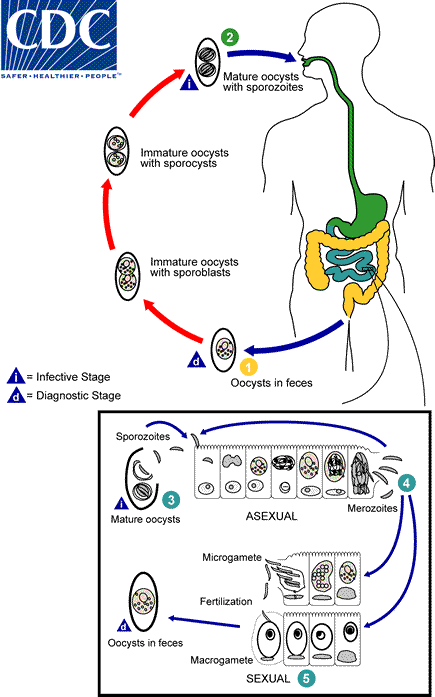
\includegraphics[width=0.85\columnwidth]{A.imagenes/ACV-BioSan-Parasit-CbelliCbios}
		\caption[Ciclo biológico y morfología de \textit{C. belli}]{Ciclo biológico y morfología de \textit{C. belli}. Vehículo: agua o alimentos contaminados, Vía: oral, Agente: Ooquiste.\label{fig:PARASIT:CbelliCBios}}
	\end{figure}
\end{multicols}
\subsubsection{Sintomatología y patogenia}
La cystoisosporosis tiene un periodo de incubación de 2 a 13 días, un periodo prepatente de 7 a 9 días y un periodo patente de 2 a 3 semanas (en pacientes inmunosuprimidos, es de 1 a 2 meses). Su principal acción patógena es la acción traumática (destruye los enterocitos y otras células intestinales). Este parásito se asocia a un gran número de eosinófilos y células plasmáticas.

La sintomatología es muy parecida a una gastroenteritis viral: febrícula, nauseas, vómitos, diarrea persistente pero autolimitantes (más de 10 deposiciones diarias), siendo estas, a veces, de aspecto grasiento y líquido, dolor abdominal y pérdida de peso. En pacientes inmunocomprometidos, las diarreas no son limitantes, y se tiende a una invasión generalizada, una isosporidosis extraintestinal, una diseminación del parásito por los ganglios linfáticos y la muerte.
\subsubsection{Diagnóstico}
La principal técnica es el diagnóstico directo por coprología, búsqueda de ooquistes en heces. Para resaltar estas formas parasitarias, se puede optar por teñir con yodo o concentrar mediante técnicas de flotación o sedimentación. Se observan en la muestras gran cantidad de cristales de Charcot-Leyden (residuos dejados por eosinófilos al entrar en apoptosis, resultado de su gran acción frente a este tipo de parásitos).
\newpage
\subsection{\textit{Cyclospora cayetanensis}}
\subsubsection{Morfología}
Considerada  una enfermedad emergente parasitaria, es de distribución cosmopolita, muy frecuente en zonas tropicales y templadas. Presenta dos formas 
\begin{itemize}[itemsep=0pt,parsep=0pt,topsep=0pt,partopsep=0pt]
	\item \textbf{Trofozoito}: tiene forma alargada, con puntas romas en sus extremos. En su polo apical presenta el complejo apical propio del phylum Apicomplexa. Bajo este se halla un pequeño citostoma (microporo). Presenta un núcleo grande con un nucléolo grande. En su citoplasma se halla un aparato de Golgi, un retículo endoplásmico y mitocondrias. Las formas de trofozoito reciben un nombre distinto según se originen de esporogonias, gamogonias,… su localización habitual es el interior del enterocito, entrando en el mediante fagocitosis inducida, disponiéndose bajo el borde en cepillo.
	\item \textbf{Ooquiste}: fase de resistencia, presenta una cubierta externa quística protectora, con un orificio taponado (micropilo), los esporoquistes y una masa de restos de las divisiones celulares, el residuo ooquistico. Una vez maduro, ese micrópilo se abre y deja salir las fases al exterior. En el interior de estos se forman los esporoquistes, unas estructuras cubiertas por una membrana con los esporozoitos en su interior (con su forma de coccidio típica) y un residuo esporoquistico. Forman 4 esporozoitos en su interior, repartidos en dos esporoquistes a razón de 2 por esporoquiste.
\end{itemize}
\subsubsection{Ciclo biológico}
\begin{multicols}{2}
	La vía de infección de \textit{Cyclospora cayetanensis} es la ingestión de ooquistes maduros en agua o alimentos contaminados. Sigue un ciclo directo, siendo eurixeno.
	
	Los ooquistes aguantan el pH estomacal, abriéndose en el intestino. Los esporozoitos que surgen del ooquistes se pegan al epitelio intestinal, fijándose, redondeándose y provocando su endocitosis y formación de una vacuola que les engloba en el interior del enterocito. En el interior de la vacuola, por esquizogonia, comienza a multiplicarse, surgiendo hasta merozoitos por esquizonte. Cuando estos merozoitos crecen, hacen estallar a la célula, reiniciando el ciclo infectivo estos merozoitos. Tras varias esquizogonias, se da una gamogonia, siendo anisogámica: en la invasión de los enterocitos, parte de los merozoitos formaran microgametocitos (16 por merozoito) y parte formaran macrogametocitos (1 por merozoito). Los microgametocitos se liberan y, si se encuentran con un macrogametocito, ocurre la fecundación, generando un cigoto que formará un ooquiste. El ooquiste inmaduro se libera al exterior del organismo, ocurriendo ahí su maduración, formando 2 esporoquistes con un residuo ooquistico, con 2 esporozoitos en su interior.
	\columnbreak
	\begin{figure}[H]
		\centering
		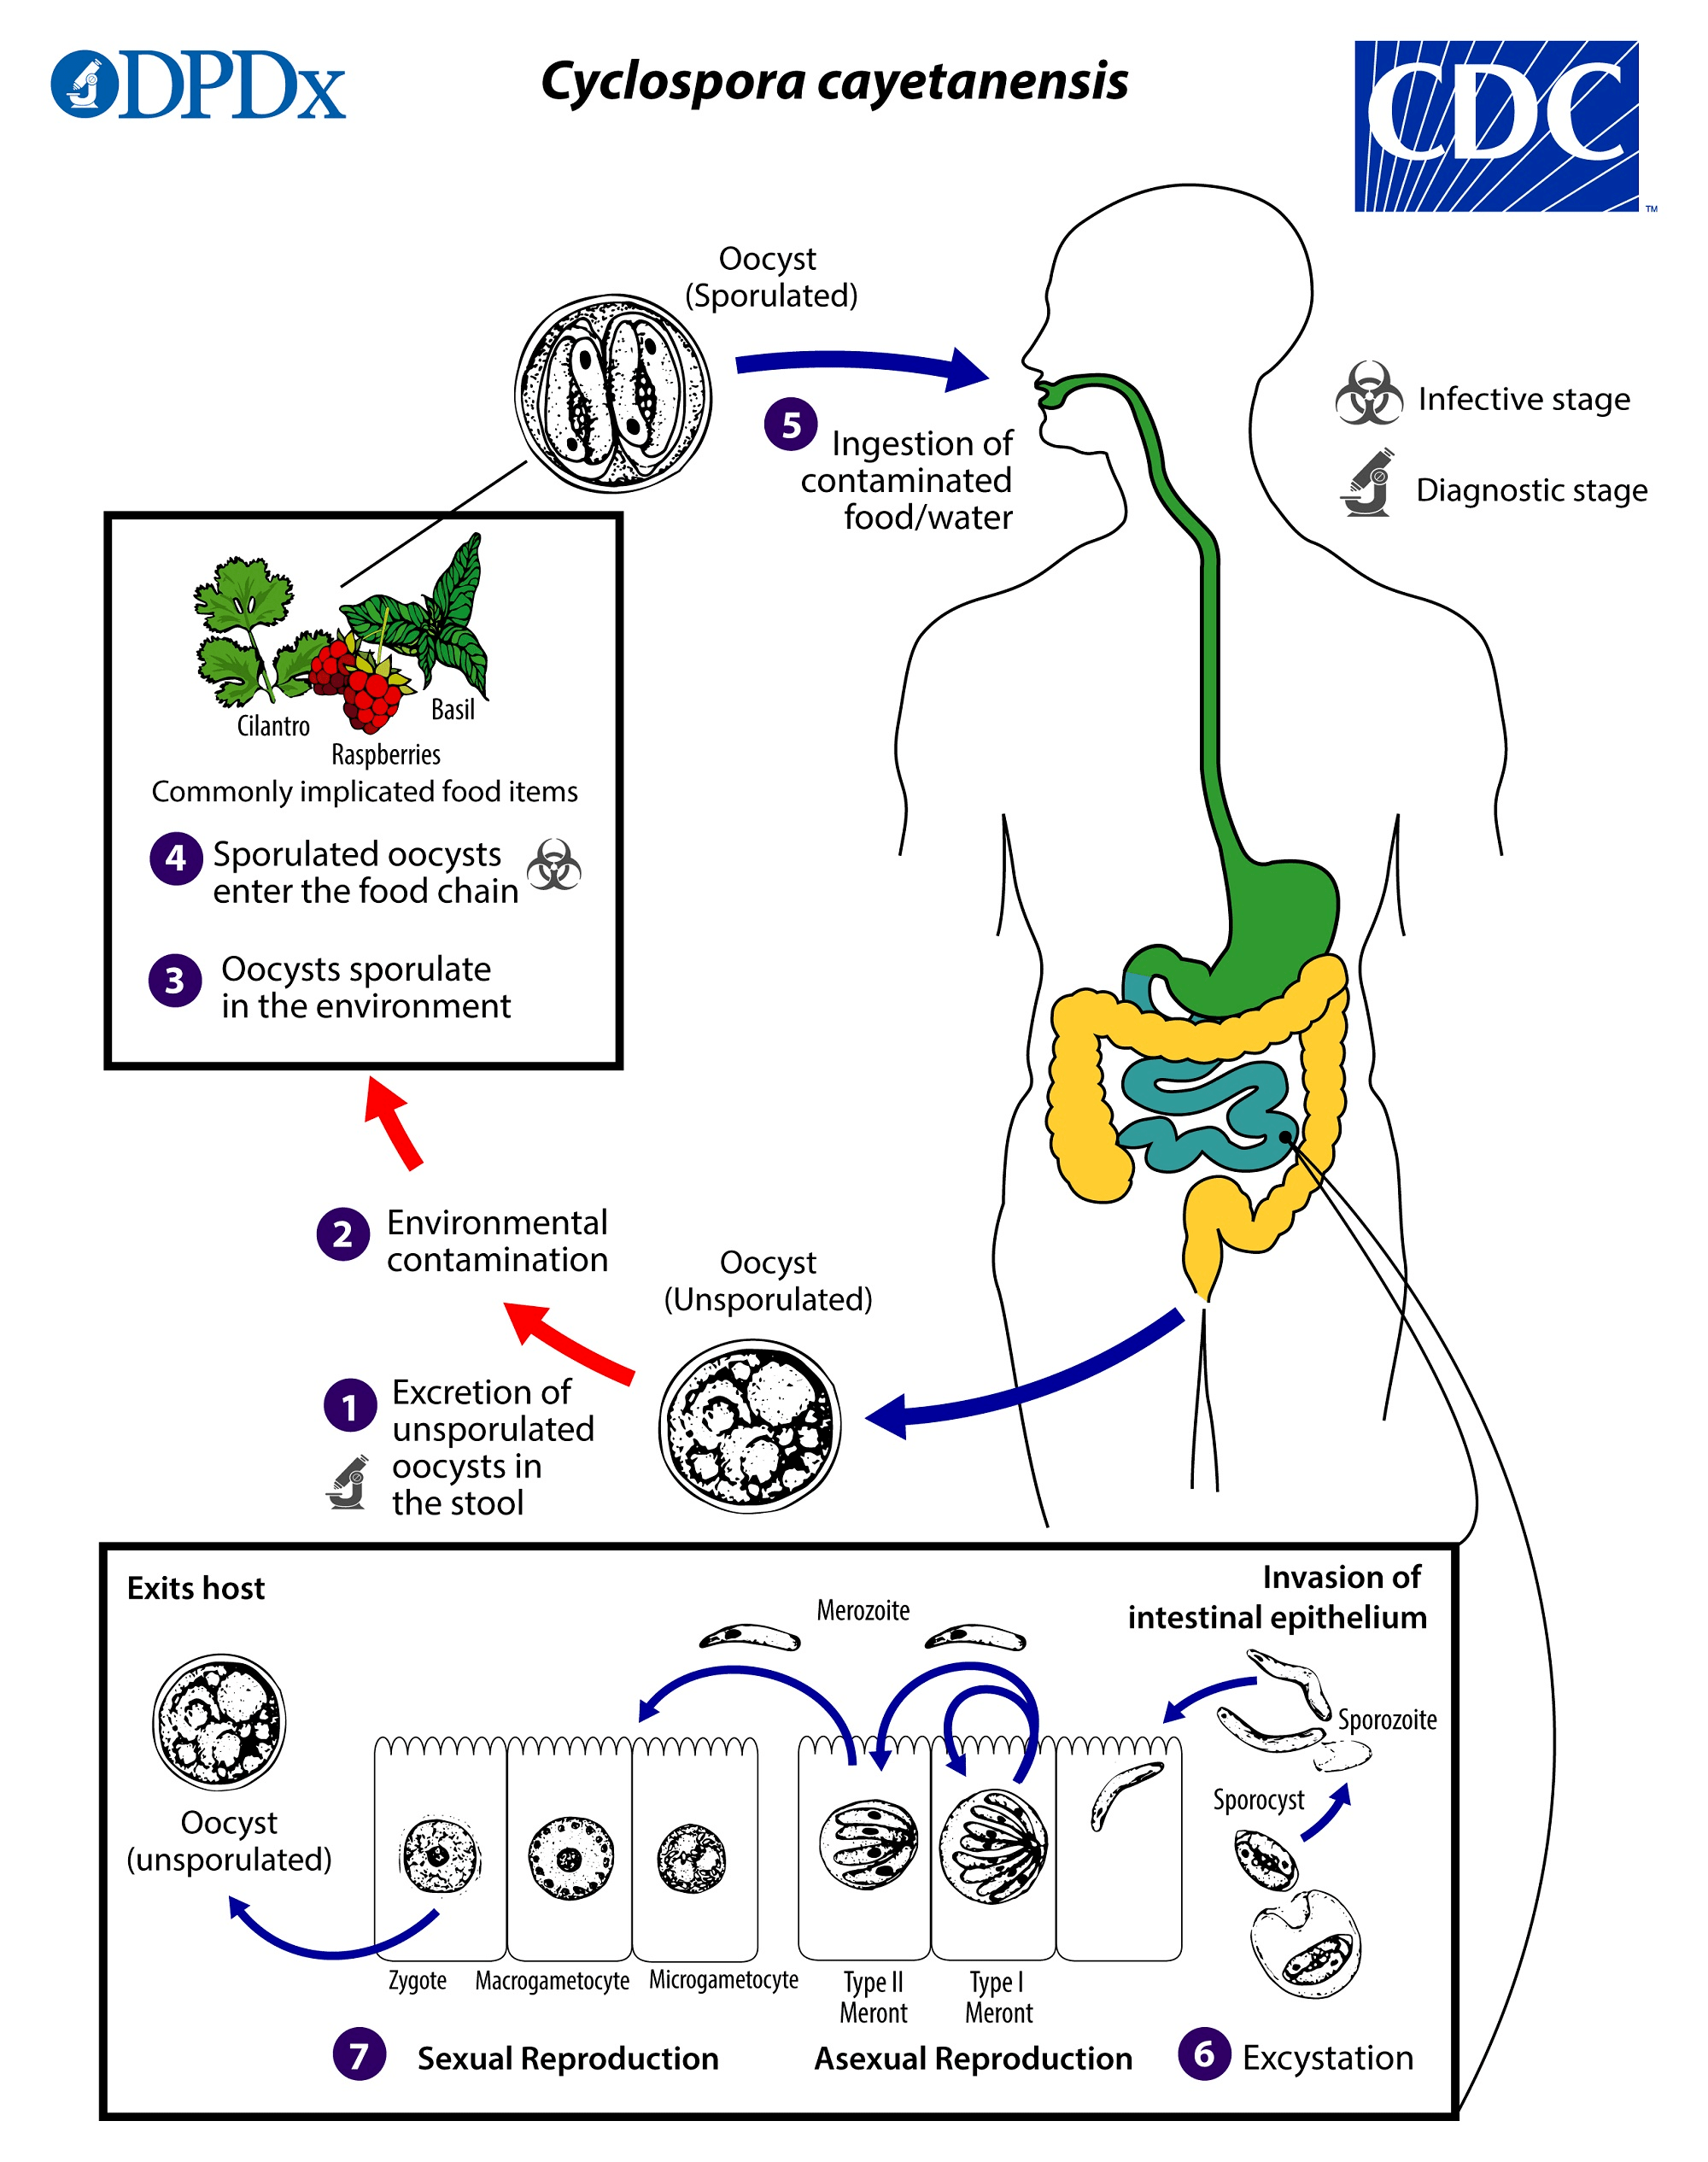
\includegraphics[width=\columnwidth]{A.imagenes/ACV-BioSan-Parasit-CcayetanensisCbios}
		\caption[Ciclo biológico y morfología de \textit{C. cayetanensis}]{Ciclo biológico y morfología de \textit{C. cayetanensis}. Vehículo: agua o alimentos contaminados, Vía: oral, Agente: Ooquiste.\label{fig:PARASIT:CcayetanesisMorf}}
	\end{figure}
\end{multicols}
\subsubsection{Patogenia y sintomatología}
La cyclosporosis provoca en el intestino una acción traumática por destrucción de las células del epitelio intestinal a la par que generan una reacción inflamatoria difusa y crónica. Todo ello genera un aplastamiento y atrofia de las vellosidades intestinales. La cyclosporosis cursa de la siguiente manera:
\begin{itemize}[itemsep=0pt,parsep=0pt,topsep=0pt,partopsep=0pt]
	\item Asintomática (se da en algunas personas, siendo portadores sanos).
	\item Sintomática, con diarreas con recaídas o cíclicas alternando con estreñimiento, pero autolimitante en inmunocompetentes, vómitos, fatiga, calambres, pérdida de peso y, en pacientes inmunosuprimidos, (VIH,…), colecistitis (por afección del conducto biliar).
\end{itemize}
\subsubsection{Diagnóstico}
La principal técnica es el diagnóstico directo por coprología, búsqueda de ooquistes en heces. Se diferencia mediante la forma y tamaño de los ooquistes (entre especies de coccidios) y por la autofluorescencia azul-verdosa bajo luz ultravioleta (característico de los coccidios).
\newpage
\subsection{\textit{Plasmodium} spp}
Paludismo, malaria o plasmodiosis son tres términos con los que se puede nombrar a la enfermedad provocada por el género de parásitos \textit{Plasmodium} spp. Estos parásitos, protozoos del phylum \textit{Apicomplexa}, familia \textit{Plasmodiidae}, presentan 5 especies capaces de infectar a los seres humanos, que son: \textit{Plasmodium vivax, P. ovale, P. falciparum, P. malariae} y \textit{P. knowlesi} (estas dos últimas parasitan al ser humano y a otros animales).
\subsubsection{Características generales}
\textit{Plasmodium} spp es un parásito que vive en la sangre, siendo un parásito intracelular de los eritrocitos. Son heteroxenos, teniendo una parte del ciclo en un hospedador intermediario (vertebrado), donde se dan procesos de esquizogonia y gametocitogénesis; y un hospedador definitivo (\textit{Anopheles}), donde se da la fecundación (final de la gamogonia) y la esporogonia. Frente a otras especies, el zigoto de este parásito es móvil, llamándose ooquineto. Todas las fases de este parásito ocurren, bien en el mosquito, bien en el vertebrado, es decir, no tiene fases de vida fuera del hospedador. Esta familia produce, por degradación de la hemoglobina, el pigmento palúdico, un pirógeno de gran importancia.

Las distintas especies se distribuyen de la siguiente forma:
\begin{itemize}[itemsep=0pt,parsep=0pt,topsep=0pt,partopsep=0pt]
	\item\textit{P. vivax}: Asia y Norte de África (34\% de casos de paludismo)
	\item\textit{P. ovale}: trópicos, EEUU, India e Indochina (poco frecuente)
	\item\textit{P. malariae}: cosmopolita (7\% de los casos)
	\item\textit{P. falciparum}: cosmopolita (50\% de los casos)
	\item\textit{P. knowlesi}: Sudeste asiático. Sin datos de prevalencia.
\end{itemize}

Antiguamente, dada la presencia de \textit{Anopheles} en las orillas del Mediterráneo, esta enfermedad también era endémica de estos países, dándose por controlada en torno a los años 60. No obstante, se han vuelto a dar casos de paludismo en estos países (Grecia, Francia, España)
\subsubsection{Morfología}
Las especies de Plasmodium presentan distintas formas celulares en su ciclo vital, que, aunque algunas son ciertamente diferentes entre las especies (teniendo valor taxonómico), son estados comunes en todas las especies. Son:
\begin{enumerate}[itemsep=0pt,parsep=0pt,topsep=0pt,partopsep=0pt]
	\item\textbf{Trofozoito}: presenta la forma típica de los \textit{Apicomplexa}, diferenciándose un estado joven, normalmente en forma de anillo; y otra madura, con una vacuola pequeña y de distinta forma.
	\item\textbf{Esquizonte}: se clasifican por el número de núcleos (merozoitos en el esquizonte maduro) que pueden presentar distintas formas.
	\item\textbf{Gametocitos}: el principal recurso para la clasificación es si deforman o no el eritrocito. 
\end{enumerate}

En cuanto a las especies, se destaca la siguiente morfología:
\begin{itemize}[itemsep=0pt,parsep=0pt,topsep=0pt,partopsep=0pt]
	\item\textit{\textbf{Plasmodium falciparum}}: responsable del 99 \% de las muertes, infectando a eritrocitos jóvenes y maduros. No presentan EES, y son proclives a causar recaídas (no se elimina totalmente al parásito, quedando a niveles que no dan síntomas). Es capaz de poliparasitar en glóbulos rojos. El trofozoito presenta forma de anillo con dos puntos de cromatina que protruyen al exterior en su fase juvenil. En su fase madura, y hasta la liberación de los merozoitos, el glóbulo rojo presenta unos gránulos, llamados de Maurer. El esquizonte (la esquizogonia dura entre 36-48 h), en su fase inmadura, almacena el pigmento palúdico en su centro. Se divide en de 8 a 32 merozoitos. El gametocito deforma el glóbulo, siendo el macho redondeado por los bordes, y el macrogametocito tiene forma de media luna.
	\item\textit{\textbf{Plasmodium vivax}}: Infecta a eritrocitos jóvenes, y realiza EES (causa de las recidivas). El trofozoito inmaduro es muy activo, presenta a veces dos puntos de cromatina y con dos anillos. El trofozoito maduro forma en el interior del hematíe unas granulaciones, los gránulos de Schuffner. La esquizogonia (de hasta 48 h) termina con entre 12 a 18 merozoitos y la hipertrofia del glóbulo rojo. El esquizonte inmaduro divide el citoplasma del eritrocito, teniendo forma irregular. El microgametocito ocupa todo el glóbulo rojo y lo no deforma, mientras que el macrogametocito es ovalado y deforma al hematíe.
	\item\textit{\textbf{Plasmodium malariae}}: No presentan EES, y son proclives a causar recaídas (no se elimina totalmente al parásito, quedando a niveles que no dan síntomas). Su parasitemia es baja, al sólo parasitar glóbulos rojos maduros. Su esquizogonia dura 72 horas.  El trofozoito tiene la forma típica de anillo, con una vacuola pequeña y el núcleo protruyendo hacia el interior. El trofozoito maduro tiene forma de prisma, y el eritrocito presenta los gránulos de Ziemann. El esquizonte inmaduro, que no deforma al hematíe, se divide en 8 merozoitos periféricos y el pigmento palúdico en el centro. Ninguno de los gametocitos deforma al glóbulo rojo, ocupándolo en su totalidad. 
	\item\textit{\textbf{Plasmodium ovale}}: Infecta a eritrocitos jóvenes, y realiza EES (causa de las recidivas). El trofozoito joven forma un anillo imperfecto, así como darse casos de poliparasitismo. En esta fase ya se encuentran presentes unos gránulos, los gránulos de Schuffer. El esquizonte acaba por formar de 6 a 12 merozoitos. Los gametocitos tienen formas redondeadas y ligeramente amorfas, deformantes del eritrocito.
	\item\textit{\textbf{Plasmodium knowlesi}}: suele parasitar simios, se confunde con otras especies por su morfología (con \textit{P. malariae}, al ser iguales sus trofozoitos maduros, y con P. falciparum, en el caso de los trofozoitos jóvenes). Su esquizogonia es la de menor duración, 24 horas (picos de fiebre diarios).
\end{itemize}
\begin{figure}[H]
	\centering
	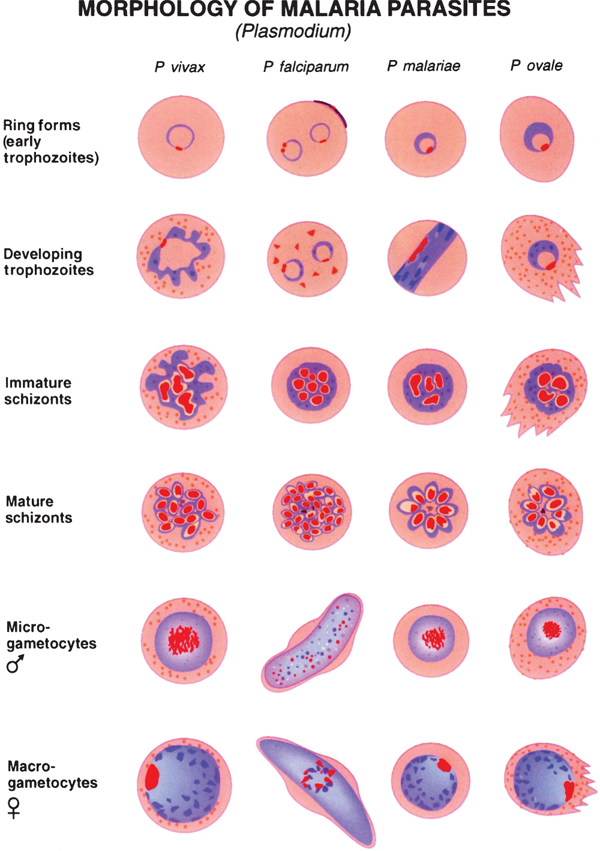
\includegraphics[trim=0 0 0 2cm,clip,width=0.75\columnwidth]{A.imagenes/ACV-BioSan-Parasit-PlasmodiumMorf}
	\caption[Morfología de las distintas especies de \textit{Plasmodium}]{Morfología de las distintas especies de \textit{Plasmodium} en las diferentes fases del parásito y su parasitación en el eritrocito, con las consecuencias de esta relación. \textit{P. falciparum} tiene poliparasitismo en su fas de trofozoito (conocido como gránulos de Maurer en esta fase), forma de 8 a 32 merozoitos deformando los eritrocitos. \textit{P. vivax} forma dos glóbulos de cromatina, y forma lo que se conocen como gránulos de Schuffner, y genera de 12 a 18 merozoitos. \textit{P. malariae} forma un nuclo no saliente y una vacuola pequeña, produciendo lo que se denominan gránulos de Zieman y forma 8 merozoitos en el eritrocito. Por último \textit{P. ovale} genera gránulos de Schuffner en su forma de trofozoito, y se forman de 6 a 12 merozoitos.}
\end{figure}
\subsubsection{Ciclo biológico}
El ciclo biológico comienza con la picadura de una hembra de \textit{Anopheles} spp parasitada inocula, junto con su saliva, esporozoitos en la sangre del hospedador intermediario. Desde la picadura, tarda unos 15 min. en llegar al hígado, entrando en los hepatocitos. En el interior de estas células, de los hepatocitos, pueden darse dos comportamientos: que \textit{Plasmodium} realice una esquizogonia (EEP: Esquizogonia Exoeritrocítica Primaria) en el hepatocito, denominada esa fase <<criptozoito>>, saliendo a posteriori al exterior cientos de merozoitos (<<metacriptozoitos>>); o que estos parásitos se queden en letargo (al hepatocito se le denomina <<hipnozoitos>>), dándose a posteriori una esquizogonia que los reactive (EES: Esquizogonia Exoeritrocítica Secundaria).

El metacriptozoito en sangre penetra en los eritrocitos (que le proporcionan un lugar de aislamiento del sistema inmune y elementos necesarios en su nutrición (hemoglobina)). En el interior de estos, toma una nueva forma, la de trofozoito, que tiene dos subfases, la de trofozoito joven, y la de maduro. Esta última, que produce el pigmento palúdico, comienza una nueva esquizogonia (el tiempo que tarda en realizar esta fase depende de cada especie), formándose el esquizonte en el interior del glóbulo rojo. Una vez que se forman los merozoitos, por presión, el eritrocito estalla, liberándolos junto con el pigmento palúdico (lo que se relaciona con los picos de fiebre de esta enfermedad: producidos por el pigmento palúdico y la propia parasitemia), pudiendo seguir estos merozoitos dos caminos: reiniciar la fase eritrocítica en otro glóbulo rojo; o comenzar una fase de gametocitogénesis en el interior de otros glóbulos rojos, diferenciándose en ellos en micro y macrogametocitos.

Cuando una hembra de \textit{Anopheles} pica a un individuo infectado, es capaz de incorporar a su interior a esos gametocitos. En su estómago, se rompen los eritrocitos y salen estos gametocitos. Los microgametocitos, por exflagelación, se transforman en microgametos; mientras que los macrogametocitos se diferencian en macrogametos. De la unión de estos, por el proceso de fecundación, continuación de la fase de reproducción sexual (gamogonia), se forma el zigoto, ooquineto. Este viaja por la pared externa del estómago, redondeándose y formando una membrana alrededor, formándose el ooquiste. Este ooquiste, por esporogonia, forma directamente esporozoitos (no hay forma intermedia de esporoquistes). Estos esporozoitos se reparten por todo el organismo del mosquito, llegando a la glándulas salivales del mosquito, pudiéndose reiniciar el ciclo con otra nueva picadura.
\begin{figure}[H]
	\centering
	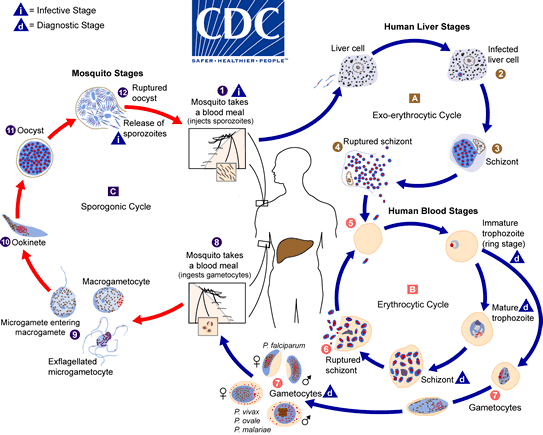
\includegraphics[width=0.85\columnwidth]{A.imagenes/ACV-BioSan-Parasit-PlasmodiumCbios}
	\caption[Ciclo vital de las distintas especies de \textit{Plasmodium}]{Ciclo vital de las distintas especies de \textit{Plasmodium}. Vector: mosquito \textit{Anopheles}. Vía: parenteral. Agente: esporozoito.}
\end{figure}
\subsubsection{Vías de transmisión}
\begin{itemize}[itemsep=0pt,parsep=0pt,topsep=0pt,partopsep=0pt]
	\item Picadura del mosquito \textit{Anopheles}, de la hembra de especies que lo puedan transmitir y que estén infectadas. Este es un riesgo presente en aeropuertos (que pasen mosquitos en el pasaje)
	\item Vía congénita (de madres no inmunes, por rotura de la placenta).
	\item Jeringuillas contaminadas
	\item Transfusiones de sangre o por trasplantes (suele ser frecuente en casos de riñón, corazón e hígado, órganos muy inervados). Este mecanismo es común en todas las especies.
\end{itemize}

En cuanto a la relación entre hospedador y parásito, se diferencian cuatro comportamientos:
\begin{itemize}[itemsep=0pt,parsep=0pt,topsep=0pt,partopsep=0pt]
	\item El parásito es incapaz de establecerse: esto ocurre en el caso de la no posesión de la proteína Duffy del eritrocito; déficit de la glucosa-6-P deshidrogenasa; talasemia; anemia falciforme o tenencia de una hemoglobina alterada.
	\item El parásito mata al hospedador: es el caso de \textit{P. falciparum}, que es mortal para personas de riesgo (inmunocomprometidos, viajeros o gente que no posee inmunidad, embarazadas, niños,$\dots$)
	\item El hospedador mata al parásito: es el caso de lactantes con madres con inmunidad frente al parasito.
	\item Parasitismo próspero o semiinmunidad: generación de portadores asintomáticos, o en fases paroxísticas.
\end{itemize}
\subsubsection{Patogenia}
Las distintas acciones que lleva a cabo el parásito son:
\begin{itemize}[itemsep=0pt,parsep=0pt,topsep=0pt,partopsep=0pt]
	\item \textbf{Traumática} de ruptura, por lisis de los eritrocitos.
	\item \textbf{Expoliadora} específica, al capturar la hemoglobina de los glóbulos rojos.
	\item \textbf{Tóxica}: genera fiebre por la propia parasitemia y por la liberación del pigmento palúdico.
	\item \textbf{Mecánica}: bloquea los capilares sanguíneos por la adsorción por parte de todo tipo de eritrocitos (sanos o infectados) que los hace propensos a pegarse en los capilares
\end{itemize}

La presencia de antígenos solubles en suero provocará una reacción inmune exagerada que se manifestará en forma de una respuesta inflamatoria exagerada, una inmunopatología. Así mismo, esos antígenos presentes en los eritrocitos, estén sanos o infectados, provocará una reacción de lisis de los mismos por acción de células del sistema inmune.

La enfermedad provocada por \textit{Plasmodium}, generará dos tipos de daños: los producidos por el parásito en su ciclo biológico, y los generados por la repuesta inflamatoria exagerada (escalofríos, fiebre, procesos autoinmunes). Así, se diferencian dos tipos de malaria: malaria no complicada (malestar con fiebre y síntomas inespecíficos) y malaria severa (que lleva a la muerte si un rápido diagnóstico).

En cuanto a los periodos de incubación, patente y prepatente, se existen diferencias entre las especies:
\begin{itemize}[itemsep=0pt,parsep=0pt,topsep=0pt,partopsep=0pt]
	\item\textbf{Periodo de incubación}: puede ir desde los 7 días (\textit{P. falciparum}); 18 días (\textit{P. vivax, P. ovale}) o hasta 42 días (\textit{P. malariae})
	\item\textbf{Periodo patente}: es de 8 días en todas las especies, excepto \textit{P. malariae}, que es de 17 a 37 días.
	\item\textbf{Periodo patente}: el lapso puede ser desde 1.5 años (\textit{P. falciparum}); 5 años (\textit{P. vivax, P. ovale}) o hasta 30 años (\textit{P. malariae}). En casos de malaria severa, puede ser de entre 28 y 42 días, dependiendo de la especie.
\end{itemize}

Según los síntomas, la malaria tiene dos fases diferenciables, que se explican según el ciclo vital del parasito. Estas son:
\begin{itemize}
	\item \textbf{Fase exoeritrocítica}: acontece la multiplicación de \textit{Plasmodium} spp. en el interior de los hepatocitos. Dura de 8 a 42 días, según la especie, y es una fase asintomática.
	\item\textbf{Fase eritrocítica}: es la fase de multiplicación del metacriptozoito en el interior del glóbulo rojo. La destrucción de los eritrocitos conlleva a una anemia (descenso de los niveles de hierro y hemoglobina) y una hipertrofia del bazo en pos de aumentar el número de células sanguíneas. En los casos de paludismo por \textit{P. falciparum}, existe, por un proceso de eritrofagocitosis provocada por la adsorción de antígenos solubles a la membrana plasmática de glóbulos rojos sanos y parasitados, un bloqueo de microcapilares, que puede desembocar en una trombosis cerebral.
	La hemoglobina libre, que se metaboliza en bilirrubina que provoca un daño hepático al metabolizarla en el hígado, apareciendo la ictericia. Esto, la bilirrubina, junto con el pigmento palúdico, que tiende a acumularse en hígado, bazo y cerebro, provoca graves brotes de fiebre de aparición cíclica. La destrucción de los eritrocitos y liberación de hemoglobina provoca una anoxemia (descenso del O$_2$ en sangre) y con ello, una hipoxia en todos los órganos y tejidos, provocando daño suprarrenal, hepático, esplénico, gastrointestinal (otro síntoma de malaria pueden ser heces con sangre o vómitos con sangre), cerebral y pulmonar.
\end{itemize}
\subsubsection{Sintomatología}
El paludismo se caracteriza por manifestarse en fases asintomáticas y sintomáticas, por lo que se le nombró en un principio como <<fiebres tercianas>> (ciclos de 48 días) o <<fiebres cuartanas>> (ciclos de 72 horas). Estas fases con sintomatología se denominan ataque palúdico, fases paroxísticas de la enfermedad con elevaciones bruscas de la temperatura. Duran de 8 a 12 horas y comienzan de la siguiente forma:
\begin{enumerate}[itemsep=0pt,parsep=0pt,topsep=0pt,partopsep=0pt]
	\item El enfermo comienza a sentir un frío intenso, escalofríos y comienza a subirle la temperatura.
	\item Cuando la fiebre llega a los 40 o hasta 42ºC, se dan síntomas de delirio, nauseas, vómitos y fortísimas convulsiones.
	\item Se da un periodo de intensa sudoración y una bajada de la fiebre, que dura unas 2 ó 3 horas.
	\item El paciente se duerme y se despierta sin ningún malestar.
\end{enumerate}

Estos ataques palúdicos pueden empezar con ciertos síntomas previos (febrículas, malestar,etc. síntomas vagos) o tener un inicio brusco. Cada ataque palúdico coincide con un ciclo de esquizogonia en el glóbulo rojo. Estas fases se repetirán, dependiendo de la especie, cada 24 (\textit{P. knowlesi}), 48 (\textit{P. vivax, P. ovale, P. falciparum}) o 72 horas (\textit{P. malariae}).

Una de las especies de Plasmodium más agresivas es \textit{P. falciparum}, del cual se deben mencionar dos clases de paludismo especial asociados a este parásito:
\begin{itemize}[itemsep=0pt,parsep=0pt,topsep=0pt,partopsep=0pt]
	\item \textbf{Paludismo cerebral}: conduce a la muerte en poco tiempo, si no hay un rápido tratamiento. Sus síntomas son: ceguera, epilepsia, ataque renal, esplenomegalia enorme, hepatomegalia e ictericia, cefalea progresiva hasta llegar al coma y fiebre superior a los 42ºC.
	\item \textbf{Paludismo congénito}: es raro, y el más asociado a esta patología es \textit{P. falciparum}. Aparece cuando la placenta está dañada (generalmente es el propio parasito el que rompe la placenta) y se adquiere en el momento del parto. Es muy frecuente en madres no inmunes, por el curso más severo de la enfermedad en ellas, que afecta a la placenta.
\end{itemize}
\subsubsection{Inmunidad}
La semiinmunidad se relaciona con una exposición intensa y prolongada en áreas de malaria endémica, con una transmisión persistente. Así mismo, esta se desarrolla de forma lenta, en torno a 5 ó 10 años, siendo esta no permanente (se puede perder cuando el individuo semiinmune deja de estar expuesto). Mantiene la enfermedad de forma asintomática, protege frente a la malaria severa, pero no evita la infección, dejándola a niveles submicroscópicos, apenas detectables, pero que los hace transformarse en portadores asintomáticos.

En cuanto a la respuesta inmune, la parasitemia provoca la producción de IgG y de la estimulación de linfocitos T CD4 y CD8 en sangre e hígado respectivamente. Esta última es el tipo de inmunidad (la inmunidad celular) la más efectiva cuando \textit{Plasmodium} está en el interior de la célula.
\subsection{Diagnóstico}
Se pueden llevar a cabo las siguientes técnicas:
\begin{itemize}[itemsep=0pt,parsep=0pt,topsep=0pt,partopsep=0pt]
	\item \textbf{Diagnóstico etiológico}: mediante análisis de sangre, se puede localizar mediante dos técnicas:
	\begin{itemize}
		\item Por frotis teñidos con Giemsa (tan solo se localizan en concentraciones mayores a los 5 o 16 parásitos/$\mu$L)
		\item Por gota gruesa: se depositan tres gotas de sangre sobre un porta (técnica de concentración), remover en un área de unos 2 cm$^2$ durante 30 segundos para desfibrinar, secar y limpiar. Posteriormente se tiñe con Giemsa sin fijar con metanol.
	\end{itemize}
	\item \textbf{Diagnóstico indirecto}: ya sea mediante técnicas serológicas (IFI,$\dots$) o por tiras cromatográficas reactivas, inmunocromatografía (útiles en campañas epidemiológicas por su rapidez y bajo coste)
	\item \textbf{PCR}: de gran sensibilidad y especificidad (cercanas al 100\%), identifican la especie, así como permiten diagnosticarlo cuando se hallan en concentraciones muy bajas (hasta 0.002 parásitos/$\mu$L).
\end{itemize}
\newpage
\subsection{\textit{Toxoplasma gondii}}
Toxoplasma gondii es un parásito del filo \textit{Apicomplexa} con distribución cosmopolita, que varía su prevalencia e incidencia según las costumbres culinarias de la zona. Es más incidente en aquellas zonas donde es costumbre cocinar poco la carne, mientras que en zonas donde es costumbre hacerlo en gran medida, es poco común.

El parásito fue descubierto en 1908, en 1937 fue descrita su transmisión congénita, pero hasta 1965 no se supo todas las fases y hospedadores de su ciclo vital.
\subsubsection{Morfología}
Según su estado de desarrollo, se diferencian tres estados:
\begin{itemize}[itemsep=0pt,parsep=0pt,topsep=0pt,partopsep=0pt]
	\item \textbf{Esporozoitos}: taquizoitos con mayor número de rotrias y micronemas. Surgen por esporogonia. Contenidos dentro de los ooquistes (uno en los inmaduros,  dos en los maduros), la maduración de estos ooquistes acontece en el exterior. Se destruyen con calor.
	\item \textbf{Taquizoitos}: originados por endopoligenia, tienen una morfología muy similar a la del coccidio típico. No resisten la digestión en el estómago, pero se multiplican rápidamente. Con forma de media luna, tras la multiplicación por endopoligenia, se multiplican rápidamente y se diseminan por el organismo. Son capaces de atravesar la placenta.
	\item \textbf{Bradizoitos}: surgen por endodiogenia, proceso más lento, son las formas presentes en infecciones crónicas, dado que son las formas que se hallan en los quistes tisulares de \textit{T. gondii}. Resisten la digestión, no se activan salvo inmunosupresión. No son capaces de sobrevivir a temperaturas de más de 65º o menores a -20ºC.
\end{itemize}
\begin{figure}[H]
	\centering
	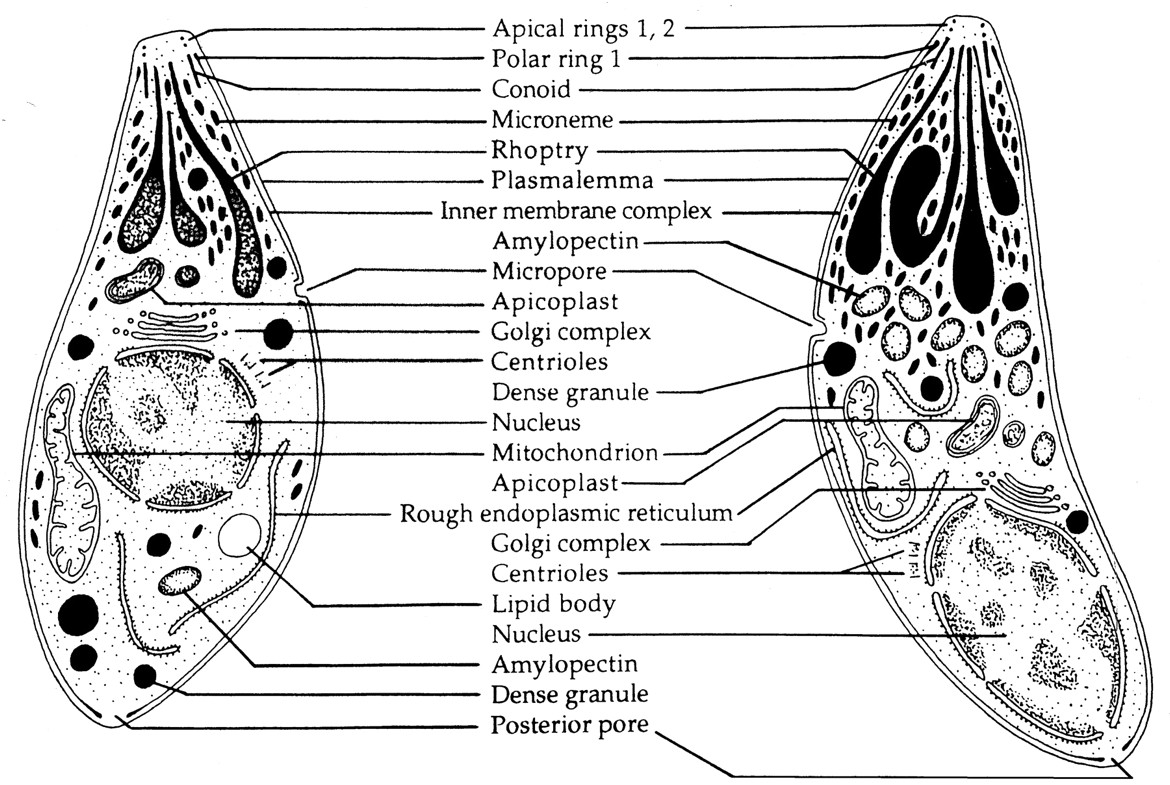
\includegraphics[width=0.7\columnwidth]{A.imagenes/ACV-BioSan-Parasit-TgondiiMorf}
	\caption[Morfología de \textit{T. gondii}]{Comparativa de las formas de taquizoito y bradizoito de \textit{T. gondii}.}
\end{figure}
\subsubsection{Ciclo biológico}
El ciclo comienza tras la gamogonia, en el intestino del hospedador definitivo, el gato. Tras este proceso de reproducción sexual, comienza la esporogonia, saliendo al exterior los ooquistes inmaduros. De 1 a 5 días, de un esporozonte se obtienen dos esporoquistes, con 4 esporozoitos cada uno y el residuo esporoquistico. Estos esporozoitos son infectantes para todos los hospedadores. 

Los hospedadores intermediarios se infectan, bien por la ingesta de ooquistes maduros como a partir de la ingesta de bradizoitos presentes en carnes contaminadas, pasando al intestino delgado. Allí, penetran y se dirigen al endotelio de los capilares sanguíneos por un proceso de endopoligenia. Así, se forman taquizoitos, que se dispersan por los tejidos, infectando a las células, introduciéndose dentro de una vacuola. A esa célula infectada se le denomina pseudoquiste. Allí, por endopoligenia, se forman más taquizoitos, que, tras muchas multiplicaciones, hacen estallar la célula y se liberan. Así, continúan durante 3 semanas, tras las cuales surge una respuesta inmune, momento en el que el parásito se queda confinado a células nerviosas, del ojo y fibras musculares, donde, por endodiogenia, se multiplica y transforma en bradizoitos. El consumo por parte de otro hospedador dará lugar a una reiniciación del ciclo o, en el gato, la terminación del ciclo.

Estos <<zoitos>>, en el gato (pasan por consumo de carne contaminada (ratones, fundamentalmente) se reproducen, en los enterocitos del intestino delgado del gato por endopoligenia, endodiogenia y esquizogonia. Los merozoitos que surgen de este último proceso, la esporogonia, comienzan la reproducción sexual: la gamogonia. Una serie de células en microgametocitos, otras células, en macrogametocitos. Tras la fecundación, se obtiene un zigoto que forma el esporonte del ooquiste inmaduro.

La infección en el gato dependerá de la forma parasitaria que ha ingerido. La forma de esporozoito tiene un periodo prepatente de unos 20 días. Los taquizoitos, de menos de 19 días, y los quistes, de 3 a 10 días. También es importante señalar la importancia de una vía congénita de transmisión del parásito, solo posible cuando está en fase de taquizoito (antes de la inmunidad).
\begin{figure}[H]
	\centering
	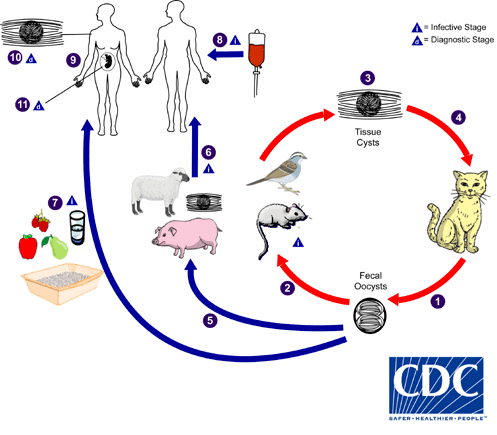
\includegraphics[width=0.7\columnwidth]{A.imagenes/ACV-BioSan-Parasit-TgondiiCbios}
	\caption[Ciclo biológico de \textit{T. gondii}]{Ciclo biológico de \textit{T. gondii}.Vehículo: agua o alimentos contaminados, Vía: oral, parenteral o placentaria, Agente: cualquier fase. El único hospedador definitivo conocido es miembros de la familia \textit{Felidae}. (1): los ooquistes no esporulados salen de las heces del gato. Aunque estos tardan de 1 a 2 semanas en madurar, se generan en gran cantidad. Tras 1 o 5 días, los ooquistes maduran en el ambiente, comenzando a ser infecciosos. Los hospedadores intermedios naturales (pájaros y roedores) se infectan por agua o alimentos contaminados. (2 y 3): los ooquistes se transforman en en taquizoitos, que se localizan en tejidos nervioso y muscular y se transforman en bradizoitos. (4): Los gatos se infectan por la ingestión de estos hospedadores infectados, repitiendo el ciclo. Los seres humanos se infectan, siendo un hospedador intermedio no esperado, infectandos por la ingestión de carne contaminada con el parásito (5 y 6); alimentos contaminados (7), transfusiones y via placentaria (8 y 9). En el ser humano, el parásito repite el patrón de los hospedadores intermedios, pero nunca terminará el ciclo.}
\end{figure}
\subsubsection{Vías de transmisión y control}
Para el hospedador intermedio (el hospedador definitivo se contagia por el consumo de carne contaminada con bradizoitos, normalmente, aunque las tres fases le resultan infectantes), se transmite:
\begin{itemize}[itemsep=0pt,parsep=0pt,topsep=0pt,partopsep=0pt]
	\item \textbf{Ingestión} de carne poco cocinada contaminada con quistes con bradizoitos.
	\item \textbf{Ingestión} de agua o verduras con ooquistes maduros (esporozoitos).
	\item \textbf{Transfusiones}, vía trasplacentaria o durante la lactancia (taquizoitos).
\end{itemize}

Así, los elementos de control son:
\begin{itemize}[itemsep=0pt,parsep=0pt,topsep=0pt,partopsep=0pt]
	\item Rápida eliminación de heces de gatos.
	\item Limpieza de vegetales crudos.
	\item Guantes para manipular heces.
	\item Cocinado de los alimentos a más de 66º o congelación a menos de -20º.
	\item Diagnóstico precoz en el embarazo (importantes son los títulos límite de infección aguda y crónica y/o diagnóstico con IgM (de fases crónicas)).
\end{itemize}
\subsubsection{Patogenia y sintomatología}
El periodo de incubación de la toxoplasmosis es de 2 días, el periodo prepatente dura desde varios días a semanas, y el periodo patente se extiende durante años. 

La principal acción de \textit{Toxoplasma gondii} suele ser acción traumática por destrucción de las células que infecta (pseudoquistes) y se desarrolla. Suele cursar asintomática por lo general, dado que esa destrucción se ve compensada por la regeneración celular.

Así, la enfermedad cursa según dos periodos:
\begin{enumerate}[itemsep=0pt,parsep=0pt,topsep=0pt,partopsep=0pt]
	\item \textbf{Toxoplasmosis aguda}: se manifiesta por una linfoadenopatía de los ganglios cervicales (90\% de los casos), siendo estos duros y dolorosos. Esta linfoadenopatía se acompaña de fiebre, malestar general, cansancio, dolores musculares y de cabeza. En algunos casos, la patología se complica con afecciones del SNC (4.3\%), miocarditis (1.4\%) y neumonía (0.8\%).
	\item \textbf{Toxoplasmosis crónica}: a las tres semanas de la infección crónica, comienza la fase crónica, con un desarrollo de la inmunidad frente a este parásito, pero que no le erradica. Esta fase dura meses o años. Es un periodo asintomático, en el que los quistes con bradizoitos no son nocivos salvo reactivaciones (pacientes inmunosuprimidos) que produzcan la rotura de los quistes y la liberación de los bradizoitos. La multiplicación de los bradizoitos origina focos de necrosis e inflación, provocando, en la retina, ceguera, o fallos en distintos órganos y, por ello, muerte.
\end{enumerate}

La toxoplasmosis también puede transmitirse por vía congénita (toxoplasmosis congénita o  subaguda). Por vía placentaria llega hasta el feto, desarrollándose de forma anómala. La tasa de infección a medida que avanza el embarazo es inversamente proporcional a los daños producidos en el feto. Así, durante el primer trimestre, tan solo se infecta el 14\% de los expuestos, cursando con daños letales al feto y abortos. En el segundo, esa tasa es del 29\%, y en el tercero, del 59\%. En estos casos, los daños no son letales, pero provocan ciertos problemas neurológicos. Así, \textit{T. gondii} causa los siguientes daños: hidrocefalia, problemas neurológicos, esplenomegalia, hepatomegalia, calcificaciones en el SNC, convulsiones.
\subsubsection{Diagnóstico}
Dada la imposibilidad de realizar un diagnóstico directo, se realizan las siguientes pruebas:
\begin{itemize}[itemsep=0pt,parsep=0pt,topsep=0pt,partopsep=0pt]
	\item \textbf{Dye-test} o \textbf{Técnica de Sabin-Feldman}: para ella se usan \textit{T. gondii} vivos, a los que se les cultiva con el suero problema (se busca saber si hay anticuerpos contra \textit{T. gondii} en él, indicativo de presencia) y azul de metileno a 37ºC durante 30 minutos. Se estudia morfología (el parásito se deforma si es positivo a la presencia de anticuerpos), movilidad (positivo si son inmóviles) y sensibilidad a la tinción (si es positivo, no se colorean).
	\item \textbf{Inmunodiagnóstico}: sin riesgo de manipulación, se hace mediante técnicas de IFI, ELISA, HAI, pudiéndose además obtener datos cuantitativos. Dado que la evolución de los anticuerpos es la de repetir una campana de Gauss, los datos pueden tomarse de forma errónea en métodos cuantitativos, se recomienda, una vez realizada la medición, o repetirla a los 21 días, o realizarla con anti-IgM, que indican curso agudo y no pueden atravesar la placenta. Así mismo, se ha de contar con que \textit{T. gondii} posee autofluorescencia azul, luego se ha de eliminar mediante la adición de azul Evans, que enmascara esa característica.
	\item \textbf{Aislado y cultivo} (necropsias).
	\item\textbf{PCR}
\end{itemize}
\newpage
\subsection{\textit{Eimeria}}
    % SEC III - Platelmintos
     \chapter{\textit{Phylum Plathelmintes}}

Los trematodos son una clase de gusanos planos (Platyhelmintes) de simetría bilateral, cuerpo aplanado dorsiventralmente, foliáceo, con aparato digestivo bifurcado, sin aparato respiratorio ni circulatorio, mayoritariamente hermafroditas y con ventosas como órgano de fijación.

Diastema hace referencia a la posesión de dos ventosas (oral y ventral) de estos géneros.
\newpage
\section{Clase \textit{Cestoda}}
\subsection{\textit{Taeniarrynchus}}
Los tenidos son una familia incluida dentro da la clase Cestoda, una división del phylum Platyhelminthes. Estas especies cuentan con una serie de características comunes:
a) Son gusanos planos de forma alargada o de cinta con segmentación corporal.
b) Ausencia de aparato digestivo. Se alimentan a través del tegumento.
c) La mayoría son hermafroditas.
d) El cuerpo está dividido en tres partes perfectamente distinguibles:
• Escólex: región más anterior, en él se encuentran los órganos de fijación.
• Cuello: región proliferativa de los distintos anillo o proglótides.
• Estróbilo: conjunto de los proglótides.

Morfología
Taeniarrynchus saginatus

Taeniarrynchus saginatus, o Taenia saginata, es un gusano parásito del intestino humano en su forma adulta y de la musculatura de otros animales en su fase larvaria. De hasta 12 metros de longitud, llega tener hasta 2000 anillos formando su estróbilo. 

Presenta un escólex inerme (róstelo sin ganchos) con 4 ventosas grandes y poco salientes. Este escólex tiene forma de priesma rectangular, siendo más ancho que alto. Sigue a esta estructura el cuello, donde no se pueden distinguir estructuras con las tinciones de rutina, siendo la zona de proliferación de los proglótides. Los anillos del estróbilo se dividen en dos tipos:
• Maduros: forman la parte más proximal del estróbilo. Planos, cuadrangulares, poseen de 300 a 400 testículos. Los anillos poseen un único poro genital, que se abre de forma alterna e irregular a un lado u otro. A este salen, por un lado, la vagina con esfínter), que asciende hasta bifurcarse en el ootipo (donde acontece la fecundación), en la glándula vitelógena (estructura más inferior del proglótide) y en el ovario, que es bilobulado (superior a las estructuras anteriores, ambos lóbulos son iguales). Sobre el ootipo surge el útero, ramificado a ambos lados, con de 15 a 30 pares de ramas uterinas. Del poro genital también surge el vaso deferente, que termina en la bolsa del cirro, de donde surge el cirro o pene, y que comienza en las vesículas testiculares por fusión de sendos vasos deferentes. En su exterior se encuentran, de exterior a interior, y en ambos lados, un nervio y el canal excretor, que se une por medio de una unión transversal (basal al proglótide) con el del otro lado.
• Grávido: tan solo se halla el útero, repleto de huevos. El resto de estructuras han degenerado.

Otras fases larvarias son:
• Huevo: esférico, sin opérculo ni espolón, presentan una doble corona radiada (embióforo) con un embrión (oncosfera) completamente desarrollado, con tres pares de ganchos (hexacanto). Fase de eliminación en el hospedador definitivo.
• Cisticerco o metacestodo: presente en la musculatura del hospedador intermediario, se trata de una vesícula de ligero color rosado (mioglobina) con el escólex invaginado.

Taenia solium

Taenia solium, o “solitaria”, es un gusano parásito del intestino humano en su forma adulta y de la musculatura de otros animales en su fase larvaria. De hasta 7 metros de longitud, llega tener hasta 700 o incluso 1000 anillos formando su estróbilo. 

Presenta un escólex armado (róstelo con doble corona de ganchos en forma de “navaja” o “pinza de cangrejo”) con 4 ventosas grandes y poco salientes. Este escólex tiene forma piriforme. Sigue a esta estructura el cuello, donde no se pueden distinguir estructuras con las tinciones de rutina, siendo la zona de proliferación de los proglótides. Los anillos del estróbilo se dividen en dos tipos:
• Maduros: forman la parte más proximal del estróbilo. Planos, cuadrangulares, poseen de 100 a 150 testículos. Los anillos poseen un único poro genital, que se abre de forma alterna e irregular a un lado u otro. A este salen, por un lado, la vagina (sin esfínter), que asciende hasta bifurcarse en el ootipo (donde acontece la fecundación), en la glándula vitelógena (estructura más inferior del proglótide) y en el ovario, que es trilobulado (superior a las estructuras anteriores, con dos lóbulos iguales y uno tercero muy poco perceptible). Sobre el ootipo surge el útero, ramificado a ambos lados, con de 7 a 14 pares de ramas uterinas. Del poro genital también surge el vaso deferente, que termina en la bolsa del cirro, de donde surge el cirro o pene, y que comienza en las vesículas testiculares por fusión de sendos vasos deferentes. En su exterior se encuentran, de exterior a interior, y en ambos lados, un nervio y el canal excretor, que se une por medio de una unión transversal (basal al proglótide) con el del otro lado.
• Grávido: tan solo se halla el útero, repleto de huevos. El resto de estructuras han degenerado.

Otras fases larvarias son:
• Huevo: esférico, sin opérculo ni espolón, presentan una doble corona radiada (embrióforo) con un embrión (oncosfera) completamente desarrollado, con tres pares de ganchos (hexacanto). Fase de eliminación en el hospedador definitivo.
• Cisticerco o metacestodo: presente en la musculatura del hospedador intermediario, se trata de una vesícula de ligero color rosado (mioglobina) con el escólex invaginado.


Ciclo biológico
Taenia saginata

Parásito heteroxeno, tiene un hospedador definitivo (el ser humano) y uno intermediario (ganado bovino). Es cosmopolita.

El ciclo comienza con la fecundación de los proglótides (mediante autofecundación o entre proglótides distintos), pasando el anillo maduro a su estado grávido, con el consiguiente aumento del útero y la degeneración del resto de estructuras. Tras ello, se desprende del estróbilo (tras 2 o tres meses se observan formas de eliminación) de uno en uno, pudiendo forzar el esfínter anal en su salida. 

En el exterior, por la temperatura y la labilidad del proglótide, se rompe y libera los huevos. Si en esa zona está el hospedador intermediario (por ejemplo, pastos de los que se alimenta el ganado bovino) puede ingerir los huevos, contaminándose. La cubierta radiada les protege del ácido estomacal, rompiéndose el embrióforo en el duodeno, surgiendo la oncosfera. La oncosfera, por medio de sus ganchos rompe la pared intestinal y busca un capilar, por el que viajará normalmente a la musculatura del hospedador. Allí acontece el proceso de vesiculización: el parásito entra en una de esas células, transformándose en un cisticerco (Cysticercus bovis). Cuando el hospedador definitivo ingiere la carne contaminada, este pasa por el estómago sin problemas y llega al duodeno, donde se evagina el escólex del cisticerco, rompiéndose la vesícula que lo protegía, y se fija a la mucosa intestinal. Allí crece, en un proceso conocido como estrobilización, donde llega a su forma definitiva de adulto, pudiéndose cerrar el ciclo.

Taenia solium

El ciclo comienza con la fecundación de los proglótides (mediante autofecundación o entre proglótides distintos), pasando el anillo maduro a su estado grávido, con el consiguiente aumento del útero y la degeneración del resto de estructuras. Tras ello, se desprende del estróbilo (tras 2 o tres meses se observan formas de eliminación) en segmentos de 3 a 6 anillos con las heces (no fuerzan el esfínter anal). 

En el exterior, por la temperatura y la labilidad del proglótide, se rompe y libera los huevos. Si en esa zona está el hospedador intermediario (por ejemplo, pastos de los que se alimenta el ganado bovino, ovino o porcino) puede ingerir los huevos, contaminándose. La cubierta radiada les protege del ácido estomacal, rompiéndose el embrióforo en el duodeno, surgiendo la oncosfera. La oncosfera, por medio de sus ganchos rompe la pared intestinal y busca un capilar, por el que viajará a tejidos subcutáneos, musculatura, ojo y cerebro. En estos órganos acontece el proceso de vesiculización: el parásito entra en estas células, transformándose en un cisticerco (Cysticercus cellulosae, o C. racemosus (en el cerebro)). Cuando el hospedador definitivo ingiere la carne contaminada, este pasa por el estómago sin problemas y llega al duodeno, donde se evagina el escólex del cisticerco, rompiéndose la vesícula que lo protegía, y se fija a la mucosa intestinal. Allí crece, en un proceso conocido como estrobilización, donde llega a su forma definitiva de adulto, pudiéndose cerrar el ciclo.

En esta especie existe la posibilidad de que el sr humano se comporte como hospedador intermediario, esto es, se infecte con el huevo y desarrolle cisticercos. Existen dos vías para ello: infestación heterógena (ingiera huevos en agua o alimentos); o autógena (exógena, vía ano-mano-boca; o por antipersitaltismo, que lleve a los anillos al duodeno y allí emerjan). 



















Taenia asiatica

Descubierta en 1993, presenta la misma morfología que T. saginatus, aunque presenta un ciclo parecido al de T. solium. El hombre se infecta mediante la ingestión de cisticercos de esta especie presentes en el hígado de cerdo (hospedador intermediario). Se distribuye fundamentalmente por las costas orientales de Asia. Dado que solo es distinguible a nivel molecular, no se sabe mayor información de este helminto.

Control:
• Lavado correcto de ensaladas.
• A nivel del hospedador definitivo: control de excretas y diagnóstico y tratamiento de hospedadores.
• Con respecto a hospedadores intermediarios: congelado y/o cocinado de la carne y control veterinario de la misma.

Teniosis

La teniosis es la enfermedad provocada por la fase adulta de T. saginata, y T. solium. Su periodo de incubación es de 2 meses, su periodo prepatente de 2 a 3 meses, y el patente, de 25 años. Este parásito lleva a cabo las siguientes acciones:
• Traumática: debido al rostelo (ventosas y ganchos), que rompe la submucosa y provoca una inflamación local.
• Tóxica: llevado a cabo por subproductos del metabolismo del parásito, que provocan prurito anal.

Los síntomas suelen ser muy leves, pudiéndose incluso dudar se estos no están influenciados por el nerviosismo del paciente al conocer al parásito. Estos son: dolores epigástricos, molestias abdominales, vómitos, diarreas, pérdida de apetito, pérdida de peso y prurito anal.



Cisticercosis

Causada por la forma de cisticerco de Taenia solium. Su periodo de incubación depende del órgano afectado, siendo antes en tejidos cerebrales, ojo, submucosa y, por último, músculo. Su periodo de incubación es de 2 a 3 meses, su periodo prepatente de 2 meses y el patente, 2 años. Las acciones que realiza son:
• Mecánica: de gran importancia en el cerebro, al bloquear ciertas regiones.
• Tóxica: sobre todo es importante en el músculo, al producir inflamación y calcificación.

Los síntomas dependen del tipo de cisticercosis:
• Cerebral: dependiente de la localización: cefalea, convulsiones, cambios de personalidad, delirios de grandeza, pérdida de visión, crisis epileptiformes, etc.
• Ocular: molestias oculares, pérdida de visión.
• Musculares: miosistis.

Diagnóstico

• Teniosis: tan sólo se puede recurrir al diagnóstico etiológico por coprología, ya sea visualizando los anillos grávidos, clasificando la especie según el número de ramas uterinas; o visualizando los huevos, sin posibilidad de clasificción dentro de los Ténidos.
• Cisticercosis: Mediante inmunoensayo (HAI, ELISA); o por técnicas de imagen (detección del cisitcerco (etiológico y clínico)): Rayos X, TAC, Escáner.
\newpage
\subsection{\textit{Hymenolepididae}}
Morfología

La familia Hymenolepididae es una familia de tenias cosmopolitas muy frecuente en niños, pero no tanto en adultos, que suelen ser inmunes. De esta familia, presentan repercusión sanitaria Hymenolepis nana e H. diminuta. Ambos son cestodos pequeños, con las siguientes características:
• Hymenolepis nana: de 0.7 a 10 cm, el adulto presenta un escólex globoso con rostelo armado (una corona, en forma de horquilla) y retráctil, un cuello muy marcado y 4 ventosas. Los anillos son más anchos que largos, con un solo aparato genital masculino y femenino. El poro genital es lateral, que se continúa con una vagina y un útero (saciforme), y sólo tres testículos.
El huevo es completo sin embrióforo radiado, en forma de limón con de 4 a 8 filamentos polares.
Presenta una forma de cisticercoide: una forma sólida (constituye la cola, situada en el extremo posterior) y una forma vesiculosa (estructura globosa donde se halla invaginado el escólex del adulto).
• Hymenolepis diminuta: de 20 a 50 cm, el adulto presenta un escólex globoso con rostelo inerme y retráctil, un cuello muy marcado y 4 ventosas. Los anillos son más anchos que largos, con un solo aparato genital masculino y femenino. El poro genital es lateral, que se continúa con una vagina y un útero (saciforme), y sólo tres testículos.
El huevo es completo sin embrióforo radiado, esférico y sin filamentos polares. Es mayor que H. nana.
Presenta una forma de cisticercoide: una forma sólida (constituye la cola, situada en el extremo posterior) y una forma vesiculosa (estructura globosa donde se halla invaginado el escólex del adulto).
Ciclo biológico

Se trata de un parásito heteroxeno con un hospedador intermediario, los redores, y ocasionalmente el ser humano (accidental, actúa como hospedador definitivo o intermediario). De la siguiente forma, presenta dos ciclos: indirecto y directo.

• Ciclo directo: sólo presente en H. nana, en el hospedador definitivo; acontece de la siguiente manera. Los huevos eliminados por el adulto pueden generar una autoinfección exógena (vía ano-mano-boca o vehiculizados en agua o verduras contaminadas) o endógena (huevos que eclosionan en el intestino). Fuera como fuere, entre las vellosidades intestinales se libera la oncosfera y acontece la vesicularización, formando, en este caso, un cisticercoide sin cola (tardando 4 días). Una vez completado el proceso, el cisticercoide se libera al lumen, donde se evagina, asciende hacia el duodeno y comienza la estrobilización. 

• Ciclo indirecto: presente en ambas especies, necesita de un hospedador intermediario y uno definitivo. El proceso es el siguiente:
Tras la fecundación de los proglótides maduros, se liberan los anillos grávidos, que al ser tan lábiles, se rompen antes de salir, siendo únicamente los huevos vehiculizados al exterior. Allí, estos huevos esperan al hospedador intermediario, que habrá de ingerirles. Lo hacen las fases larvarias de una pulga o de un colóptero, continuando el ciclo, por ser hospedadores intermediarios. Es necesario que el aparato bucal sea masticador y no picador para poder ser introducidos al intestino de estos animales.

En el interior de estos hospedadores intermediarios (situados en el ambiente del roedor, siempre cercano a depósitos de grano), la oncosfera, rompe las cubiertas que le protege, abandona el intestino de estos insectos y se establece en el hemocele de estos. Allí se transforman en cisticercoides y permanecen al encuentro con el hospedador definitivo.

La entrada al hospedador definitivo se produce cuando un roedor o el ser humano ingieren, de forma accidental, a estos insectos. En el intestino de estos hospedadores definitivos acontece la salida del cisticerocide, la evaginación del escólex y, una vez fijado a la pared intestinal, la estobilización 


Control:
• A nivel de hospedador intermediario, desinsectación (normalmente zonas próximas a graneros, cuyos trabajadores son población de riesgo)
• A nivel de hospedador definitivo, desratización y diagnóstico y tratamiento de hospedadores, así como una correcta higiene personal.

Hymenolepiosis

El periodo de incubación de la hymenolepiosis es de 1 a 4 semanas, el periodo prepatente de 2 semanas, y el patente, de 2 a 4 semanas. El parásito lleva a cabo las siguientes acciones:
• Traumática: generada por la oncosfera, cuyos ganchos provocan, sobre la mucosa intestinal, una reacción inflamatoria local, pero el movimiento de los adultos (no se sitúan siempre en el mismo lugar), que no poseen ganchos pero si ventosas, extiende por varios sitios esa inflamación.
• Tóxica: provocada por los metabolitos expulsados por este gusano platelminto.

La patogenia de este parásito consiste en el aplanamiento de las vellosidades por los cisticercoides (autoinfestación) y una enteritis superficial sin llegar a generar úlceras en la mucosa si existe una gran cantidad de parásitos. Esta parasitosis puede cursar de dos formas distintas:
• En adultos suele ser asintomática.
• En niños, por el ciclo de autoinfección, suelen ser masivas, mostrando: malnutrición, dolor abdominal, diarrea por aumento del peristaltismo, prurito anal y nasal (acción tóxica), nerviosismo (genera meteorismo, pérdida de peso y crisis epileptiformes).
Diagnóstico

• Etiológico: mediante coprología (visibles los huevos en heces por gran cantidad (infestaciones masivas) y el aspecto característico de los huevos.

\newpage
\subsection{\textit{Diphilium caninum}}
Morfología

Cestodo intestinal del perro y el ser humano (ocasionalmente). Llega a medir de 20 a 80 centímetros y tiene un diámetro de, en torno a 3 ó 5 mm. Presenta las siguientes fases en su ciclo biológico:
• Adulto: presenta un escólex globoso con 4 ventosas de gran tamaño y un rostelo piramidal y armado con de 3 a 7 coronas de ganchos en espinal de rosal (triangulares). A esta región le sigue el cuello y el estróbilo. En esta última, el estróbilo, presenta anillos maduros (en forma de tonel, presenta una simetría bilateral: tiene dos poros genitales en sendos lados, apatri de los cuales se localiza una vagina, un ovario y una glándula vitelógena postovárica. Junto al poro genital surge la bolsa del cirro, que se continúa con el vaso deferente, que se ramifica para ir a los 150 a 300 testículos presentes) y grávidos (en forma de tonel, presenta un útero muy desarrollado que se divide en cápsulas ovíferas en cuyo interior se hallan presentes los huevos).
• Huevo: presenta el huevo típico de los ténidos: un embrión hexacanto en su interior (tres pares de ganchos) y un embrióforo no radiado. Es completo, presentando dos cubiertas.
• Cisticercoide: presenta una forma sólida (constituye la cola, situada en el extremo posterior) y una forma vesiculosa (estructura globosa donde se halla invaginado el escólex del adulto).

Ciclo biológico

El ciclo comienza tras la autofecundación de los proglótides maduros, formándose los anillos grávidos, que son expulsados en grupos de 5 a 6 de forma activa (fuerzan el esfínter anal). En el exterior, los anillos se rompen y se liberan las cápsulas ovíferas, que son capaces de resistir hasta 25 días. Cuando una de estas es ingerida por una fase larvaria de una pulga (Ctenocephallides canis, Ctenocephallides felis) o un piojo masticador adulto (Trichodectes canis) del perro, continua el ciclo, por ser hospedadores intermediarios. Es necesario que el aparato bucal sea masticador y no picador para poder ser introducidos al intestino de estos animales.

En el interior de estos hospedadores intermediarios (situados en el ambiente del perro), la oncosfera, rompe las cubiertas que le protege, abandona el intestino de estos insectos y se establece en el hemocele de estos. Allí se transforman en cisticercoides (suele haber de 10 a 60 de estos) y permanecen al encuentro con el hospedador definitivo.

La entrada al hospedador definitivo se produce cuando el perro o el ser humano ingieren, de forma accidental, a estos insectos. En el intestino de estos hospedadores definitivos acontece la salida del cisticerocide, la evaginación del escólex y, una vez fijado a la pared intestinal, la estobilización 

Control:
• A nivel de hospedador intermediario: desinsectación de perro y entorno.
• A nivel de hospedador definitivo: diagnóstico y tratamiento de individuos parasitados.

Dypilidiosis

La dypilidiosis es una enfermedad que en adultos suele cursar de forma asintomática, así como ser especialmente poco frecuente; pero en niños, y debido a, principalmente, la acción tóxica del parásito, generada por la eliminación de metabolitos tóxicos para el organismo. Los síntomas son: anorexia, diarrea, pérdida de peso, prurito anal, nerviosismo y crisis epileptiformes.

Diagnóstico

• Etiológico: mediante coprología (visionado de huevos, cápsulas ovíferas o anillos en heces) u observación de cápsulas ovíferas en camas de gatos o entornos a animales de compañía (textura similar a arena blanquecina).
\newpage
\subsection{\textit{Echinococcus granulosus}}
Morfología

Gusano cestodo, parasito cosmopolita eurixeno. Presenta una forma adulta, presente en el intestino del perro (hospedador definitivo), y unas fases larvarias que están en los distintos hospedadores intermediarios.
• Adulto: de pequeño tamaño (hasta 7 mm), su cuerpo está formado por un escólex con 4 ventosas y un rostelo piriforme con una doble corona de ganchos en forma de puñal; un estróbilo de 2 a 3 anillos (inmaduro, maduro y grávido). El anillo maduro posee un ovario en forma de riñón, glándula vitelógena postovárica, entre 25 a 80 testículos y un poro genital en la mitad posterior. Los anillos grávidos tienen un útero longitudinal con cortas ramificaciones.
• Huevos: igual que el de otros ténidos: esférico, sin opérculo ni espolón, presentan una doble corona radiada (embrióforo) con un embrión (oncosfera) completamente desarrollado, con tres pares de ganchos (hexacanto). Fase de eliminación en el hospedador definitivo.
• Protoescólex: fase larvaria presente en el hospedador intermediario, si se halla invaginado tiene forma de grano de café con los ganchos muy marcados. Cuando se evagina, tiene la forma del escólex del adulto.

Otra formación que genera el parásito es el quiste hidatídico: En el órgano donde se asiente la oncosfera formará una cápsula formada por una membrana laminar (externa) y una germinativa (interna), de la cual saldrán las cápsulas prolígeras, con los protoescolex en su interior. En el interior de la capsula están los protoescólex libres, vesículas hijas endógenas viables o no, y restos degenerados de otras estructuras. Por acción del sistema inmune, se forma una membrana adventicia, formada por el parénquima del órgano que infectan, friable de las otras dos membranas. Estos pueden ser infértiles (sin protescólex), fértiles (con protoescólex) o hiperfértiles (con muchas vesículas hijas); o degenerado (calcificado).

Ciclo biológico

El ciclo biológico comienza en el intestino del perro, el hospedador definitivo, con la salida de los huevos del anillo grávido, saliendo los huevos, ya embrionados, por las heces. Estos contaminan el pasto donde pacen los hospedadores intermediarios: ovejas, cerdos, reses,…

En el intestino de los hospedadores intermediarios, el embrióforo se rompe y surge la oncosfera, que rompe la pared intestinal en su búsqueda de un capilar, donde viajará a distintos órganos, preferentemente hígado y pulmones, pero pudiendo llegar a corazón, interior de huesos y cerebro. Allí formarán el quiste hidatídico

El ciclo es continúa cuando el hospedador definitivo ingiere las vísceras del hospedador intermediario contaminadas con estos quistes hidatídicos. El protoescólex, que se halla invaginado, aguanta el paso por el estómago y se evagina en el duodeno del perro. Aquí, se ancla con sus ventosas y su rostelo a la pared intestinal. Allí acontece el proceso de estrobilización y, una vez formados los anillos, se produce la fecundación, cerrándose el ciclo.
En este caso, el humano es un hospedador accidental, actuando como hospedador intermediario, contaminándose por huevos presentes en comida o por presentes en el pelaje del perro que acaban por llegar a la zona oral.

Control:
• Tratamiento de hospedadores definitivos (perros)
• Control de carnes que sirvan como fuente de alimentación al perro.

Hidatidosis

Las acciones que lleva a cabo el parásito son:
• Traumática: llevada a cabo por la oncosfera, esta irrita al órgano en el que está, formando una membrana adventicia sobre el parásito.
• Mecánica: la lleva a cabo el quiste generando una presión contra el órgano donde se ubica. Resulta más severa en el cerebro.
• Tóxica: por salidas de líquido hidatídico (que puede dar lugar a quistes secundarios), que lleva algunos metabolitos tóxicos para el hospedador. Dependiendo de la menor o mayor cantidad de líquido puede ser local (necrosis del tejido adyacente) o generalizada, que puede producir un shock anafiláctico y, con ello, la muerte.

Los síntomas suelen ser pobres, sino inexistentes, aunque depende del órgano que afecte.

Diagnóstico

• Etiológico: se realiza mediante visualización del quiste por técnicas de imagen (Rayos X, Escáner, Ecografía). Nunca se harán biopsias por riesgo a la rotura y diseminación de protoescólex.
• Inmunológico: se realiza mediante intradermoreacción de Casoni (desaconsejada, se trata de ver una reacción inmune por inoculación parenteral de antígeno del parásito; produciéndose inmunidad contra este una vez realizada la prueba), HAI, ELISA, IFI o Inmunoelectroforesis, mediante la visualización del arco 5(tiene reacciones cruzadas con E. multilocularis).
\newpage
Echinococcus multilocularis
Morfología

Gusano cestodo, parasito restringido al Hemisferio Norte (Norte de Asia, Canadá y parte de EEUU, Rusia, Alemania, Suiza, Austria; Grecia y Turquía) eurixeno. Presenta una forma adulta, presente en el intestino del perro (hospedador definitivo), y unas fases larvarias que están en los distintos hospedadores intermediarios.
• Adulto: de pequeño tamaño (hasta 5 mm), su cuerpo está formado por un escólex con 4 ventosas y un rostelo piriforme con una doble corona de ganchos en forma de puñal; un estróbilo de 4 a 5 anillos (inmaduro, 2 maduros y 2 grávidos). El anillo maduro posee un ovario en forma de bilobulado, glándula vitelógena postovárica, en torno a 20 testículos y un poro genital en la mitad anterior. Los anillos grávidos tienen un útero sacular con cortas ramificaciones.
• Huevos: igual que el de otros ténidos: esférico, sin opérculo ni espolón, presentan una doble corona radiada (embrióforo) con un embrión (oncosfera) completamente desarrollado, con tres pares de ganchos (hexacanto). Fase de eliminación en el hospedador definitivo.

• Protoescólex: fase larvaria presente en el hospedador intermediario, si se halla invaginado tiene forma de grano de café con los ganchos muy marcados. Cuando se evagina, tiene la forma del escólex del adulto.

Otra forma, sólo presente en el hospedador intermediario, es la del quiste hidatídico alveolar: forma una red de túbulos que se infiltra en el órgano. Presenta una membrana adventicia (externa) generada por el hospedador a partir del parénquima del órgano, una adventicia y otra germinativa más interna, formadas por el parásito, que forman las estructuras de protoescólex y vesículas hijas, que en el caso del ser humano, son infértiles.

Ciclo biológico

El ciclo biológico comienza en el intestino del zorro o del gato, hospedadores definitivos, con la salida de los huevos del anillo grávido, saliendo los huevos, ya embrionados, por las heces. Estos contaminan el pasto donde pacen los hospedadores intermediarios: roedores.

En el intestino de los hospedadores intermediarios, el embrióforo se rompe y surge la oncosfera, que rompe la pared intestinal en su búsqueda de un capilar, donde viajará a distintos órganos, preferentemente hígado y pulmones, pero pudiendo llegar a corazón, interior de huesos y cerebro. Allí formarán el quiste hidatídico

El ciclo es continúa cuando el hospedador definitivo ingiere las vísceras del hospedador intermediario contaminadas con estos quistes hidatídicos. El protoescólex, que se halla invaginado, aguanta el paso por el estómago y se evagina en el duodeno del zorro o del gato. Aquí, se ancla con sus ventosas y su rostelo a la pared intestinal. Allí acontece el proceso de estrobilización y, una vez formados los anillos, se produce la fecundación, cerrándose el ciclo.
En este caso, el humano es un hospedador accidental, actuando como hospedador intermediario, pero en el que las hidátides son infértiles, contaminándose por huevos presentes en comida (fresas silvestres).

Control:
• En el caso humano, no comer frutos silvestres cercanos al suelo (especialmente fresas silvestres)

Hidatidosis alveolar

De pronóstico grave, llega a ser mortal. Similar a la hidatidosis unilocular, suele formar hidátides en el hígado, pero también en el pulmón y en el cerebro. Esta enfermedad cursa con: hepatomegalia, hígado duro e irregualr a la palpación, insuficiencia hepática, ictericia, cirrosis y, en pulmón y cerebro, un crecimiento que recuerda a metástasis de algunos tumores.


Diagnóstico

El diagnóstico suele ser complejo. La forma del quiste hidatídico multilocular puede recordar a la de un tumor, no recomendándose la biopsia ante el riesgo de diseminación. Las técnicas inmunológicas más sensibles son IF, ELISA y Inmunoelectroforesis, mediante la visualización del arco 5 (tiene reacciones cruzadas con E. granulosus), pero pueden dar falsos positivos en neoplasias o de otras hidatidosis. 
\newpage
\subsection{\textit{Diphylobotium latum}}
Morfología

Descrito ya en el papiro de Ebers, se le conoce como la “tenia ancha del pez”. Suele distribuirse en aguas frías: Mar Baltico, Mar del Norte, lagos de Suiza, Mar de Barents, Mar Jónico y Tirreno y Costas del Pacífico Norte.

Llega a medir hasta 20 metros en su forma adulta, siendo lo más normal que se sitúe entre los 30 y 8 metros; se trata de un cestodo que llega a poseer hasta 3000 o 4000 proglótides. Se pueden distinguir las siguientes fases vitales en su ciclo vital:
• Adulto: presenta un escólex (pequeño, piriforme con un par de botrios laterales, sin rostelo armado); un cuello; y un estróbilo.
Los anillos maduros poseen un poro genital único y ventral y anterior al tocostoma (orificio por el que salen los huevos). El útero es central y tiene forma de roseta, mientras que el útero es bilobulado. Posee un gran número de testículos y de folículos vitelógenos, que se distribuyen por todo el anillo.
El anillo grávido  presenta un útero muy desarrollado 
• Coracidio: surgido del huevo en un ambiente acuoso, consiste en una estructura similar al embrión de un tenido (esférico, con seis pares de ganchos (embrión hexacanto)) con una capa externa de células ciliadas que le permiten nadar en ese medio.
• Larva procercoide: de aspecto alargado, presenta en su parte anterior unas glándulas de penetración y los ganchos en su parte más posterior, en un cuerpo vesiculoso surgido por estrangulamiento de esta región denominado cercómero.
• Larva plerocercoide: fase presente en el pez, es similar al adulto, presenta los botrios y una pseudometamerización en todo el cuerpo.
• Huevo: de color marrón oscuro, operculados y de extremos redondeados, sus medidas son de 71x51 $\mu$m.


Ciclo biológico

Se trata de un parásito heteroxeno y eurixeno, que sigue un ciclo con dos hospedadores intermedios y una amplia gama de hospedadores definitivos (mamíferos ictiófagos).

El ciclo comineza con la autofecundación del parásito en el intestino del hospedador definitivo. Los huevos salen por el tocostoma del anillo grávido y son vehiculizados por las heces al exterior, estando en el momento de la salida en el estado de mórula (no están embrionados). Tras caer en un medio acuático, en unos 11 a 15 días en temperaturas de 8 a 30ºC, la forma de coracidio surge del huevo. Esta forma nada en la superficie hasta que es ingerida por un copépodo de los géneros: Diaptomus, Metocyclops, Cyclops. En el interior de este se forma la larva procercoide, situándose en su intestino.

Cuando un pez de la familia de los salmónidos (lucio, perca, salmón,…) ingiere a un copépodo parasitado, se libera el procercoide en el intestino del pez y abandona este aparato en dirección a la musculatura del pez. Allí, este se transforma en plerocercoide. En ese momento puede acontecer que sea ingerido por un hospedador paraténico o por el definitivo. Cuando el hospedador definitivo ingiera la carne (del hospedador intermediario o paraténico) contaminada con esas larvas plerocercoides, en el duodeno acontecerá la estrobilización y desarrollo del parásito, cerrándose así el ciclo.
Control:
• Evitar la ingesta de pescado poco cocinado o no congelado.
• Diagnóstico y tratamiento de individuos no parasitados.
• Control de excretas.
Botriocefalosis

El periodo de incubación de la enfermedad es de 21 días; el periodo prepatente es de 21 a 24 días; y el patente, de hasta 10 años. Las principales acciones de este parásito son:
• Mecánica: al situarse en el duodeno, si la carga parasitaria es alta puede llegar a obstruir el intestino.
• Expoliadora: este parásito detenta hasta el 50% de la vitamina B12 que pasa por el intestino, impidiendo su absorción.

La mayoría de las botriocefalosis suelen ser asintomáticas (portadores sanos), pero los hospedadores sintomáticos presentan el siguiente cuadro de síntomas: diarrea, pérdida de peso y dolor abdominal; cefaleas; reacciones alérgicas; obstrucción intestinal si la carga parasitaria es alta; colecistitis o colanguitits por la migración de proglótides a regiones anteriores del intestino, donde pueden germinar; y déficit de vitamina B12, que se manifiesta con anemia y neuropatía periférica y lesiones en el SNC.

Diagnóstico

• Clínico: la presencia de anemia megaloblástica, déficit de vitamina B12 y una eosinofilia en sangre periférica (5 a 10% de los pacientes), son indicativos de una parasitemia por este gusano.
• Etiológico: mediante coprología (el hallazgo de huevos en heces se puede hacer a partir de las 6 semanas) o mediante técnicas de diagnóstico molecular diferencial entre especies (PCR).
\newpage
\section{Clase \textit{Trematoda}}
\subsection{\textit{Fasciola hepatica}}
Morfología y distribución

De gran tamaño, cosmopolita, Fasciola hepática es el agente etiológico de la fasciolosis. El adulto presenta una ventosa oral prominente en el cono apical. Ciegos intestinales ramificados, hermafroditas: su aparato reproductor lo forma un ovario ramificado, dos testículos posteriores a estos y unas glándulas vitelógenas extendidas por el margen lateral y posterior del cuerpo.

Los huevos son grandes, ovalados, simétricos y con una cáscara fina, operculado en un extremo. Las cercarias presentan un extremo anterior cónico y una cola natatoria.

Ciclo biológico

El adulto suele vivir en las vías biliares, en su parte proximal, del hospedador definitivo (cerdos, ovejas o el ser humano). En ellas se alimenta de bilis, se autofecunda y pone los huevos, que caen por el colédoco al duodeno y salen vehiculizados por las heces. Esos huevos salen no embrionados, necesitando un medio húmedo (charcos,…) para terminar de formarse. Tras 10 días, a 22ºC y por la luz, el huevo se rompe saliendo el miracidio por el opérculo, necesitando encontrar al hospedador intermediario (caracol de la familia Lymnaeidae, como Lymnaea trunculata, presente en España).El miracidio entra al hospedador intermediario por los tentáculos o por el pie. En el punto de penetración forma un esporoquiste que genera las redias madres, que buscan el hepatopáncreas, donde se forman las redias hijas, que darán lugar a las cercarias, que abandonan el caracol saliendo con el moco.

Las cercarias nadaran hasta zonas con vegetación, donde se enquistan, transformándose en metacercarias. Si son ingeridas por el hospedador definitivo, las metacercarias pasan por el estómago, liberando al trematodo joven en el duodeno. Allí rompen la mucosa dirigiéndose al peritoneo, buscando el hígado e introduciéndose en los conductos biliares, cerrándose el ciclo. No obstante, puede perderse en su viaje al hígado, encapsulándose en regiones ectópicas (pulmón,…) y calcificándose.

Control:
• Higiene alimentaria: limpieza de alimentos (especialmente berros) para ensaladas.
• Tratamiento de individuos parasitados.
• Desplazamiento del hospedador intermediario mediante molusquicidas, competencia con otras especies,…

Fasciolosis

El periodo de incubación es de 3 a 12 semanas, el prepatente de 3 meses y el patente de hasta 20 años. El parásito lleva a cabo las siguientes acciones en el hospedador:
• Traumática: se da en el hígado y en los conductos biliares por el tegumento espinoso y las ventosas del parásito y el movimiento de este en el parénquima hepático, que llevan a una reacción inflamatoria acompañada de eosinofília con una fibrosis portal e hiperplasia de los conductos biliares.
• Tóxica: por la eliminación de ciertos metabolitos que causan daño en el hospedador (prolina)
• Mecánica: obstructiva, por el bloqueo de los conductos biliares que se produce por la presencia en estos del parásito y de la hiperplasia de estos por la presencia del parásito.

Esta enfermedad se caracteriza por unos síntomas muy generales (que suelen acompañar a muchas enfermedades) y algunos más específicos hepáticos por ser este el órgano más afectado por la parasitemia. Son: dolor abdominal intenso (en las primeras semanas), cefalea intensa, vómitos, diarrea, anemia, escalofríos y gran eosinofilia, urticaria y edema submandibular, hepatomegalia dolorosa al tacto, ictericia y abscesos en lugares ectópicos.

Diagnóstico

• Clínico: por la presencia de un bloqueo hepático asociado a una hepatomegalia dolorosa, síndrome febril eosinofílico y consumo de berros.
• Etiológico: mediante la búsqueda de huevos en coprologías. Para evitar falsos positivos, se recomienda no comer hígado en los tres días anteriores a la prueba. 
• Indirecto: muy útil en el periodo prepatente, se usa HAI, ELISA o IFI.
\newpage
Morfología y distribución

La opisthorchiidosis es una parasitosis provocada por gusanos planos (platelmintos) de la familia Ophisthorchidae. En concreto, los géneros más representativos que tienen una significancia en el campo clínico son Clonorchis (C. sinensis, o “duela de China”, de Japón, Tailandia, Korea y Vietnam) y Ophisthorchis (O. felineus y O. viverrini, el primero presente en el antiguo Pacto de Varsovia; y el segundo originario de Indochina).
Ambos dos son gusanos pequeños, con forma de bala o huso (el adulto), y un huevo no distinguible.
• Adulto: todas las especies son iguales, salvo en los testículos (en Clonorchis son ramificados y en Ophisthorchis son lobulados). Posee una ventosa apical que se continúa con la faringe, el esófago y se bifurca en dos ciegos no ramificados. A los lados, en situación lateral, de los ciegos intestinales se hallan las glándulas vitelógenas. En situación medial y posterior a la bifurcación de los ciegos se halla la ventosa ventral y, posterior a ella, el útero, los ovarios y los testículos (en la posición más terminal.
• Huevo: forma esférica con un opérculo con estructuras anexas (hombros del opérculo) que lo refuerzan y un tubérculo en situación opuesta.

Estos géneros se encuentran sobre todo en Asia (Rusia Occidental y Kazajistán, China, Corea, Indochina y Filipinas). Existen unos 19 millones de casos en Asia, y casos en Europa derivados del turismo a esas zonas. En Tailandia hay hasta 6 millones de casos. En España se han encontrado fases larvarias en algunos peces.

Ciclo biológico

El parasito, en su forma adulta, vive en los conductos biliares del ser humano, siendo su hospedador definitivo. Allí, tras alimentarse de bilis, se autofecunda y realiza la puesta de huevos, que van por los conductos biliares hasta el duodeno, y de ahí, salen con las heces al exterior. Esos huevos ya están embrionados, necesitando, para seguir el ciclo, encontrar con rapidez al siguiente hospedador, un caracol del género Bithynia.

Los huevos, que llevan al miracidio, se rompen en el intestino, liberando a esa fase larvaria (el miracidio). Del tubo digestivo migrará hacia el hepatopáncreas, pero, en el momento de salir, formará un esporoquiste del que saldrán las redias madres que formarán en el hepatopáncreas a las redias hijas que se transformaran a su vez en cercarias (de parte anterior alargada y con dos formaciones oscuras en forma de ojos (oftalmocercarias) y una cola con aleta natatoria). Estas cercarias dejan el caracol saliendo junto con el moco por su superficie plantar. Para continuar el ciclo, han de encontrar al hospedador intermediario siguiente, un pez de la familia de los ciprínidos o de los salmónidos, en las siguientes 48 horas, ayudándose para un mejor contacto de un geotropismo negativo y un fototropismo positivo.

Una vez han contactado con el pez, las cercarias se introducen bajo sus escamas y se enquistan en su fase de metacercaria en la musculatura del pez. Cuando un humano ingiere la carne del pez contaminada con metacercarias, estas aguantan los jugos gástricos y en el duodeno, liberan al trematodo joven. Este busca el colédoco y se dispone en los conductos biliares, cerrando el ciclo.

Control:
• Cocinado de pescados (a más de 50ªC) o congelación (-20ºC) para la eliminación de metacercarias.
• Tratamiento de parasitados.
• Desplazamiento de hospedadores intermediarios (molusquicidas, competencia con otras especies de caracoles,…)
• Control de aguas de letrinas.
Opisthorchiisodis

El periodo de incubación de esta parasitosis es de 2 semanas; un periodo prepatente de 2 a 4 semanas y un periodo patente de 20 años. La gravedad de la parasitosis dependerá del número de parásitos (menos de 100 suele cursar asintomática) y de la duración de la misma (relacionándose con la posibilidad de sufrir hepatitis: cuanto mayor es el tiempo que existe un parasitismo, mayor es esa posibilidad).

Las acciones que realiza este parásito son las siguientes:
• Traumática: el movimiento del parásito en los conductos biliares provoca una reacción inflamatoria eosinofílica. El engrosamiento de los conductos biliares (inflamación) dará lugar a una hiperplasia adenomatosa y fibrosa en conductos pancreáticos (por localización ectópica del parásito, lo que lleva a una pancreatitis) y biliares. 
• Mecánica: de bloqueo, debido a la presencia del parasito y la inflamación de los conductos biliares y pancreáticos, que reducen el lumen y forman cálculos biliares y daños en el páncreas. 
• Tóxica: el parásito, producto de su metabolismo, desecha subproductos que resultan tóxicos para el hospedador.
• Vehiculadora: en su paso del duodeno a los conductos biliares y pancreáticos puede llevar consigo ciertas bacterias intestinales que generen enfermedades por su localización ectópica.

La enfermedad posee dos fases, en las que suele haber una gran eosinofilia (40%), y dolor hepático a la palpación. Fases:
1. Aguda: los síntomas suelen ser fiebre, diarrea, dolor epigástrico, anorexia, cirrosis portal, hepatomegalia, ictericia, esplenomegalia. Si los huevos alcanzan localizaciones ectópicas pueden causar alteraciones nerviosas, sensoriales y cardiacas. 
2. Crónica: se acompaña de apetito irregular, distensión abdominal, diarrea y edema.

La opisthorchiidosis es también un factor de riesgo ante carcinomas hepáticos.

Diagnóstico

• Etiológico: mediante búsqueda de huevos de estas especies en heces (coprología).
\newpage
\subsection{\textit{Fasciolopsis buski}}
Morfología

Gusano trematodo de Sureste asiático y Extremo Oriente, con una prevalencia de 10 millones de casos anuales y varios reservorios (perro, cerdo, gatos, conejos,…) y al hombre como hospedador definitivo. Es uno trematodo “carnoso”, por su gran grosor.

El adulto mide hasta 75 mm de longitud, 20 mm de ancho y 5 mm de grosor. Tiene el tegumento espinoso y dos ventosas, oral y ventral, esta última siendo la más grande. En la ventosa ventral se abre la boca, que se continúa con una faringe musculosa y dos ciegos intestinales longitudinales no ramificados. En los laterales se hallan las glándulas vitelógenas, que drenan a un viteloducto que acaba en el ootipo, adonde llegan óvulo y espermatozoides. Superior al ootipo es útero, que lleva los huevos al exterior por el poro genital. Los testículos se hallan muy ramificados y dispuestos postovaricamente.

Los huevos son ovalados, grandes y operculados.

Ciclo biológico

El ciclo comienza tras la autofecundación en el intestino del hospedador definitivo. En las heces del individuo son vehiculizados al exterior gran cantidad de huevos no embrionados, que tras 3 a 7 semanas en un medio acuático, forman el miracidio. Este ha de encontrar en un máximo de 48 horas al siguiente hopeddor, un caracol de los géneros Segmentia o Hippetius. Este penetra por el pie, atravesando el tegumento, momento en el que pierde el tegumento ciliado y se transforma en esporoquiste. De este surgirán las redias madres y las redias hijas, que se desarrollan en el hepatopáncreas, formando las cercarias, que salen del caracol por el moco que libera por su pie. Las cercarias nadaran hasta encontrar el pericarpo de castañas de agua, frutos de loto o raíces de bambú, donde se transformaran en metacercarias (pierden la cola y forman una cubierta resistente).

Cuando el hospedador definitivo ingiere esos frutos con el pericarpo contaminado con metacercarias, cierra el ciclo. Estas metacercarias se exquistarán en el duodeno, dad la acción de los jugos gástricos, la bilis y la temperatura, liberando al trematodo joven, que se autofecundará y dará lugar a más huevos.

Control:
• Desplazamiento del hospedador caracol mediante molusquicidas o competencia con otros caracoles.
• Saneamiento de aguas procedentes de letrinas.
• Diagnóstico y tratamiento de individuos parasitados.
• Lavado de castañas de agua, frutos de loto o raíces de bambú con hipoclorito sódico (3 gotas/1 l de agua)

Fasciolopsis

El periodo de incubación de la parasitosis es de 1 a 2 meses; el periodo prepatente es de 3 meses; y el patente, de 1 año. La acción patógena del parásito esta generada por los adultos fijados en la mucosa intestinal (duodeno), explicándose así la sintomatología:
• Acción traumática: ulceración inflamatoria del duodeno por el roce con el tegumento espinoso del parásito con posible formación de hemorragias: diarrea tóxica persistente y dolor abdominal.
• Acción mecánica obstructiva: alteran la secreción de jugos gástricos y secreción de moco. Gran número de ejemplares puede obstruir el intestino.
• Acción tóxica: sensibilización a metabolitos tóxicos del parásito: toxemia y alergia, con edema facial y en la pared abdominal.
A veces se acompaña de anorexia, náuseas y vómitos.

Diagnóstico

• Etiológico: el más concluyente (no es posible uno clínico y no hay estimulación antigénica), visionado de huevos en coprologías (sólo tras tres meses de parasitación).
\newpage
\subsection{\textit{Heterophydae}}
Morfología

Parásitos trematodos de Extremo Oriente, Delta del Nilo, Turquía, India, China Y Japón (Heterophyes heterophyes); y Siberia y Báltico (Metagonimus yokogawai). Miden en torno a 1.7 mm de largo y 0.4 mm de ancho. Los huevos de esta familia son los de los trematodos típicos, (operculados), si bien estos son más pequeños. Las especies más importantes son:
• Metagonimus yokogawai: el útero asciende hasta el poro genital (en el centro de la ventosa ventral, ligeramente inclinada y saliente por un lado). No tiene gonotilo. Las glándulas vitelógenas son posteriores y laterales. Presenta un tegumento espinoso en el tercio anterior del cuerpo. Presenta una faringe que se bifurca en dos ciegos.
• Heterophyes heterophyes: más pequeño, órganos reproductores en la parte posterior del cuerpo: testículos lobulados. El ovario tiene localización pretesticular, al igual que el ootipo, donde se forma el huevo y a partir de él, sale el utero. Este va al poro genital. Este poro genital se abre en el centro de la ventosa ventral, que se llama gonotilo.

Ciclo biológico

Este parásito tiene como hospedador definitivo al ser humano y a otros animales, como reservorios (gatos, perros, aves), siendo por ello un parásito heteroxeno.

El ciclo comienza tras la autofecundación en el intestino del hospedador definitivo: el adulto realiza la puesta de huevos (ya embrionados) que son vehiculizados con las heces hacia el exterior. Estos huevos han de ser ingeridos con rapidez por un caracol (géneros Pirinela, Cerithidia, Melania para H. hetreophyes; Semisulcospira para M. yokogawai). 

Una vez en el intestino del caracol, se libera el miracidio, que se dirigirá hacia el hepatopáncreas, pero, en el momento de salir, formará un esporoquiste del que saldrán las redias madres que formarán en el hepatopáncreas a las redias hijas que se transformaran a su vez en cercarias (de parte anterior alargada y con dos formaciones oscuras en forma de ojos (oftalmocercarias) y una cola con aleta natatoria). Estas cercarias dejan el caracol saliendo junto con el moco por su superficie plantar. Para continuar el ciclo, han de encontrar al hospedador intermediario siguiente, un pez (de agua dulce para M. yokogawai; marino para H. heterophyes).

Una vez contacta con el pez, la cercaria penetra por el tegumento, perdiendo la cola. La cercaria, en la musculatura del pez, se redondea y enquista, formando la metacercaria. Cuando el hospedador definitivo ingiere estas metacercarias, aguantan hasta llegar al duodeno, donde surge el trematodo joven, cerrando el ciclo.

Control:
• Cocinado o congelado de pescado (río o mar).
• Diagnóstico y tratamiento de personas parasitadas.
• Control de aguas residuales: saneamientos y letrinas.
• Eliminación del hospedador caracol mediante molusquicidas o competencia con otras especies.
Heterophydiosis

El periodo de incubación de esta enfermedad es de 1 a 3 semanas; el prepatente, de 5 a 10 días; y el patente, de 2 a 6 meses. La acción patógena de este parásito depende del número de adultos o huevos, del grado de penetración de estos parásitos en la pared intestinal y la reación del paciente. Las acciones que lleva a cabo en el hospedador son:
• Traumática: la pueden generar los adultos (inflaman la mucosa intestinal y generan la hipersecreción de moco, pudiendo, en casos de parasitosis masivas, generar perforaciones de las mucosas) o los huevos (pueden llegar a la sangre y generar lesiones en regiones ectópicas: corazón (reacción tisular en válvulas cardiacas) o SNC (trastornos neurológicos).

Los síntomas suelen ser diarrea crónica y dolor intestinal, pudiendo acompañarse de úlceras duodenales.

Diagnóstico

• Etiológico: mediante coprología, visionado de huevos, aunque pueden confundirse entre otros heterofídeos.
\newpage
Paragonimus westermani
Morfología

Trematodos de la familia Troglotrematidae, la especie Paragonimus westermani se distribuye por Extremo Oriente, India, Asia, África y Latinoamérica. Presenta dos formas: adulto (en el hospedador definitivo, presente en parejas con posibilidad de fecundación cruzada, encapsulados en nódulos de hasta 4 cm de diámetro) y huevo.

Tiene una forma ovoide, midiendo de 7.5 a 12 mm de longitud, 4 a 6 mm de anchura y hasta 5 mm de grosor. Con dos ventosas del mismo tamaño en región apical y ventral. Tiene unas glándulas vitelógenas muy desarrolladas que ocupan las regiones laterales. El ovario, lobulado, se halla ventrolateral, superior a los testículos, y en posición contraria al útero. El poro genital se encuentra tras la ventosa ventral. En el centro del cuerpo está la galndula excretora. Posee unos ciegos intestinales no ramificados y una faringe muy musculada.

Los huevos son ovalados, operculados, rojizos y con un engrosamiento en la cutícula opuesta al opérculo. 

Ciclo biológico

El ciclo comienza en el hospedador definitivo (ser humano y animales que se alimentan de crustáceos). En él, tras la autofecundación, se forman los huevos, que son eliminados en la expectoración (esputo) o por las heces, tras el tragado de esa expectoración. Una vez en el exterior, en un medio acuático, y tras largo tiempo (16 a 25 días, dependiendo de la temperatura) acontece el embrionado del huevo, surgiendo a posteriori el miracidio. Esta fase es temporal, teniendo que, rápidamente, encontrar al hospedador intermediario primero, un caracol de la familia Thiaridae: Semisulcospira, Potadoma, Brotia. En este penetra por el tegumento del pie.

En el punto de entrada del caracol, pierde la capa ciliada y se transforma en esporoquiste, que formará las redias madres de las que saldrán las redias hijas (que se desarrollan en el hepatopáncreas) con el moco, se expulsan las cercarias, surgidas de las redia hijas, que, por tener en este caso una cola pequeña (en botón) se les denomina microcercarias, o xifiliocercarias, por el estilete en su polo oral. Estas cercarias usaran a un cangrejo de agua dulce como segundo hospedador intermediario.

Las cercarias entran en este a través de las branquias, siendo vehiculizadas en el agua con el aspirado de agua. En las branquias, tras 6 semanas, forman una cubierta resistente, pasando a su forma de metacercaria. Si el cangrejo es ingerido por un hospedador definitivo, en el duodeno de este se rompe la metacercaria, liberando al trematodo joven, que perfora el duodeno hasta salir a la cavidad peritoneal de la que migrará al pulmón por sangre o perforando el diafragma, (los que se pierdan, formaran quistes en localizaciones ectópicas). Si es ingerido por un hospedador paraténico, el trematodo joven se enquistará en la musculatura, pudiendo resistir también a los ácidos estomacales, pudiendo ser también infectiva para el hospedador definitivo, en el que realizará el mismo proceso de migración.

Control:
• Diagnóstico y tratamiento de hospedadores definitivos
• Control de heces y esputos.
• Cocinado de la carne de cerdo (hospedador paraténico, se elimina al trematodo joven).
• Eliminación del hospedador intermediario caracol mediante molusquicidas o competencia con otros moluscos.
• Cocinado de crustáceos, no ingesta o manipulación de estos animales previo cocinado (los jugos de estos animales son capaces de llevar metacercarias).

Paragonimosis

El periodo de incubación es de 9 a 12 semanas; el periodo prepatente es de 10 a 12 semanas; y el patente, de hasta 20 años. En el organismo, el parasito lleva a cabo las siguientes acciones:
• Traumática: la realizan los adultos, genera inflamación en los pulmones, recubriéndolos, por parte del hospedador, de una capsula fibrosa. Los huevos suelen rodearse de neutrófilos y esosinófilos formando quistes o abcesos.
• Tóxica: los huevos degenrados o los adultos son capaces de generar metabolitos tóxicos que provocan urticaria, microbacesos o la formación de granulomas.

Mientras el parasito está en su fase invasiva (periodo de incubación), los hospedadores son asintomáticos. Una vez los adultos están en el pulmón se genera una reacción hística del hospedador que forma una cápsula fibrosa sobre estos parasitos y/o sus huevos, llevando a una fibrosis difusa generalizada o localizada en el pulmón. También es importante las localizaciones ectópicas del parásito, capaces de generar granulomas en otras regiones. La sintomatología asociada a esta enfermedad es:
• Pulmón: neumonía persistente, fiebre, accesos tuberculoides acompañados de tos  persistente, hemoptosis coincidente con dolor torácico opresivo, neumotórax, esputos de color amarillo, con sangre y puntos negros. Estos síntomas, asociados a la fibrosis, empeoran con el ejercicio físico.
• Abdomen: producida por la presencia de parásitos en la cavidad peritoneal: dolor abdominal, utricaria, diarreas con aparición de huevos.
• Cerebral: genrada por loaclizaciones ectópicas de huevos, dándose casos en Japón y Corea. Produce una epilepsia similar a la cisticercosis (niños menores a 15 años), y una meningitis, que, por la presión intracraneal genera: nauseas, vómitos, edema en el nervio óptico, dolor de cabeza, paralisis y coma.

Diagnostico

• Clinico: visibles los quistes nodulares mediante rayos X, TAC y Resonancia Magnética (estas dos últimas sobre todo son útiles en lesiones cerebrales). Así mismo, una gran esoinofilia (91%), leucocitosis y gran cantidad de IgE, y ciertas características del esputo (la gran cantidad de huevos) son también decisivas.

• Etiologico: búsqueda de huevos en heces, esputo o aspirado duodenal, junto con la visión de cristales de Charcot-Leyden.

• Indirecto: pueden existir reacciones cruzadas con Fasciola o Clonorchis. Se usan la técnica de ELISA, Inmunoblot, Contrainmunoelectroforesis, Fijación del complemento (muy sensible, pero muy larga) o intradermoreacción (poco aconsejable, es muy poco sensible y, una vez se ha entrado en contacto con el parásito, genera una reacción inmune).
\newpage
\subsection{\textit{Clonorchis sinensis}}
\newpage
\subsection{\textit{Schistosoma} spp}
La esquistosomosis es una enfermedad parasitaria causada por gusanos platelmintos de la clase Trematoda, siendo, los que parasitan al ser humano, cinco especies:
• Schistosoma mansoni: África y América del Sur (importada con el tráfico de esclavos).
• Schistosoma haematobium: Cuenca del Nilo y Próximo Oriente.
• Schistosoma japonicum: China, Japón y Filipinas
• Schistosoma intercalatum: África ecuatorial (de baja incidencia y restringido geográficamente, no muy prevalente)
• Schistosoma mekongi: Cuenca del Mekong: Laos, Camboya, Tailandia (de baja incidencia y restringido geográficamente, no muy prevalente)
La importancia de estas parasitosis reside en la prevalencia. Existen un total de 600 millones de personas expuestas, con unos 200 millones parasitadas, siendo 120 millones portadores sanos y 80 millones dan síntomas.

Morfología

Este género representa una excepción dentro de la familia. Estos parásitos viven en los plexos venosos del intestino o de la vejiga urinaria; son dioicos, con un gran dimorfismo sexual (la hembra es cilíndrica y el macho plano, pero forma un canal ginecóforo que alberga a la hembra durante la cópula); carecen de faringe; y presentan un aparato digestivo ciego y bifurcado con una unión cecal posterior a la ventosa ventral. Así mismo, carecen de fase de redia, teniendo una nueva fase larvaria en el hospedador definitivo, la esquistosómula.

• Huevo: ovalados, no operculados pero con un espolón lateral (S. mansoni y S. japonicum, este último poco promienente) o terminal (S. haematobium).
• Cercaria: o furcocercaria, es la fase infectiva para el hospedador definitivo. Forma libre que sale del caracol, posee una cola bifurcada natatoria que le permite buscar al siguiente hospedador, en su parte terminal. Su parte anterior lo ocupa el cuerpo de la cercaria, que posee en su extremo apical un tegumento espinoso que le ayuda a romper la piel del hospedador, junto con glándulas que segregan colagenasa y hialuronidasa.
• Esquistosómula: fase que se da en el torrente sanguíneo del hospedador definitivo, se asemeja a una cercaria sin cola (estas la pierden en el proceso de penetración. Se alimentan de plasma
• Adulto: tanto macho como hembra presentan en su extremo anterior una ventosa oral (que se continua con el esófago que se divide, previo a la ventosa ventral, en dos ciegos comunicados con una unión cecal, posterior a esta ventosa; y que continua por todo el cuerpo del animal); y una ventosa ventral, con el poro genital en su interior al que desembocan el útero o el vaso deferente, según sea hembra o macho. Las diferencias sexuales se refieren a:
• Machos: foliáceos, sus regiones laterales forman un pliegue, el canal ginecóforo, que alberga a la hembra hasta la puesta de huevos. Presenta, partiendo del poro genital, situado posterior a la ventosa ventral, un vaso deferente al que desembocan los vasos eferentes, procedentes de los testículos. El final del aparato genital lo forma el cirro esponjoso, un saliente externo que lleva el esperma al poro genital de la hembra.
• Hembras: cilíndricas, se ubican en el canal ginecóforo hasta la ovoposición. Su aparato reproductor comienza en el poro genital y se continúa con el útero, que da a un ensanchamiento (ootipo), donde se da la fecundación. Se continúa con una bifurcación que da al viteloducto (donde desembocan las glándulas vitelógenas) y al ovario, productor de óvulos. El tamaño del aparato genital tiene una significancia taxonómica, pudiendo clasificar en distintas especies según éste ocupe un tercio (S. haematobium), la mitad (S. japonicum), o dos tercios (S. mansoni) del volumen del animal.














Ciclo biológico

El ciclo comienza en el hospedador definitivo (ser humano), con la ovoposición en los plexos mesentéricos y vesicales. La eliminación del huevo (que posee ya el miracidio en su interior) se produce por rotura de los tejidos gracias a las sustancias segregadas por el espolón del huevo. Una vez ya en la orina o en el bolo fecal, sale al exterior por las excretas, teniendo que ir a un medio acuático.

El miracidio sale del huevo por rotura lateral de este a entre 25-30ºC, baja presión de oxígeno y luz. El miracidio, ciliado, busca a su hospedador intermediario, un caracol, siendo cada especie de esquistosoma específica de un género de caracol: Biomphalaria (S. mansoni); Bulinus (S. haematobium); Tricula, Oncomelania, Robertsiella (S. japonicum); penetrando por el pie o los tentáculos rompiendo el tegumento gracias a las glándulas de penetración y una papila de penetración. El miracidio posee unas características que le permiten buscarle (geotropismo negativo y fototropismo positivo). En el punto de penetración pierde los cilios y forma un esporoquiste. De ellos surge una segunda generación que se dirige al hepatopáncreas, donde se formaran la tercera generación de esporoquistes de la que saldrán las cercarias por el moco que suelta el caracol.

Las cercarias (de cola bifurcada) salen siguiendo ritmos cronobiológicos para aumentar las posibilidades de encontrar al hospedador definitivo. En el caso de humanos, abandonan los caracoles por la mañana, cuando se acerca el posible hospedador a beber agua (en roedores, por ejemplo, eso sería por la noche). Además, para favorecer el encuentro, dado que si no lo encuentra antes de las 24 horas morirá, cuentan con una serie de comportamientos: Geotropismo negativo, fototropismo y termotropismo positivo y atracción por sombras, turbulencias y sustancias de la piel. Una vez en ella, penetra activamente mediante rotura con un tegumento espinoso y glándulas de penetración. Procesos como la evaporación de gotas en piel donde esté el parasito aceleran el proceso.

En la penetración se rompe y pierde la cola, a la par que se modifica, formando la esquistosómula. Esta se dispone en las venas de los pulmones, creciendo alimentándose del plasma. Una vez maduras (25 a 48 días postinfección), se desplazan al hígado, donde se encontraran macho y hembra, acoplándose la hembra al canal ginecóforo. Esta no se soltará del macho hasta la ovoposición, donde se cierra el ciclo.

Control:
• Control de excretas y letrinas.
• Dificultar el crecimiento del hospedador intermediario (cambios en sistema de riego, desplazamiento por competencia con otra especie,…)
• Evitar bañarse en sitios contaminados o, secarse inmediatamente tras el baño.





Esquistosomosis y dermatitis causadas por Schistosoma

Las acciones que lleva a cabo el parásito en el hospedador definitivo, más en concreto en el caso humano, dependen, más que del propio parásito en sí, de la fase en la que esté, ya que estas cambian a lo largo del ciclo vital que se da dentro del hospedador. Estas son:
• Furcocercarias: lleva una doble acción conjunta traumática y tóxica, dado que perfora la piel de forma mecánica (posee un tegumento perforador) y mediante la secreción de colagenasa y hialuronidasa, que acaba por romper la piel y la formación de máculas y pápulas.
• Esquistosómulas: lleva a cabo una casi indetectable (salvo alta cantidad de parasitemia) acción expoliadora al alimentarse del plasma.
• Adultos: también dependiente del grado de parasitemia, lleva a cabo una acción mecánica de bloqueo en hígado y/o plexos venosos. También puede producir una acción expoliadora al alimentarse de sangre.
• Huevos: es la acción que más síntomas da y la más importante a nivel clínico. Realiza una doble acción mecánica y tóxica: los huevos, con el miracidio en su interior, exuda por el espolón una serie de antígenos que, bien rompen las paredes de los órganos para salir al lumen, bien desencadenan la formación de granulomas con una inmunopatología asociada: gran inflamación de la zona y la encapsulación del huevo en un granuloma.

La esquistosomosis puede cursar de una manera crónica o aguda. La forma crónica la padecen portadores sanos, no desarrollando patología alguna, produciéndose en personas inmunocompetentes de zonas endémicas. El resto de la población padece la forma aguda de la enfermedad, que recibe nombres vulgares distintos según la especie: Fiebre de Katayana (causada por S. japonicum, propia de Japón), Esquistomatosis toxémica (provocada por S. mansoni, propia de Brasil y Puerto Rico). Los síntomas son:
a) Inicio y hasta los dos meses posteriores a la infección: enfermedad febril de 3 a 10 semanas de duración (hasta la primera ovoposición).
b) Tras el inicio de las ovoposiciones, se dan síntomas abdominales: disentería con sangre y moco, vómitos, nauseas.
c) Durante toda la parasitosis: dolores similares a artritis y otros no específicos; granulomas en pared intestinal o vesical y en tejidos peritoneales; esplenomegalia; y hepatomegalia con fibrosis periportal (que lleva a hipertensión portal y dilatación de venas colaterales).

La esquistosomosis tiende a cronificarse. Su periodo de incubación es de 1 a 7 semanas (según la especie), el periodo patente de 5 a 10 semanas, y el patente, de 5 a 25 años. Además, esta enfermedad posee varios periodos de sintomatología específica, correspondientes a distintos periodos del ciclo vital parasitario:
1. Invasión: se da en el momento de la entrada de las cercarias y la migración de la esquistosómula. Se da una dermatitis en el punto de penetración y asma (esquistosómula en las venas pulmonares)
2. Maduración a adultos: se da en el momento en el que los esquistosomas adultos viajan al hígado y se aparean, tras lo cual la hembra se va al lugar de ovoposición (primera puesta). Se genera fiebre y disentería con sangre y moco. 
3. Ovoposición intensa: la hembra pone los huevos. Se forman granulomas (poliposis intestinal) con esplenomegalia y hepatomegalia.
4. Síntomas asociados a la ovoposición: la acción de las distintas fases del parásito, sobre todo del huevo, generan una fibrosis en órganos donde llegan las formas parasitarias, descompensación hepática, hematemesis e hipertensión portal grave que puede llevar al coma.

Los granulomas se producen como una reacción inmune ante la presencia del parásito, concretamente de los huevos de éste. Así, en torno al huevo se disponen, en capas concéntricas, y de interior a exterior: macrófagos, linfocitos, neutrófilos y células plasmáticas. En algunos casos, consiguen calcificarles. En otros, el huevo consigue sobrevivir.

Esquistosomosis por especie

S. mansoni
S. japonicum
S. haematobium
Localizado en el mesenterio del intestino grueso
Forma granulomas sencillos en intestino grueso (poliposis crónica)
Fibrosis portal, cirrosis y daño hepático
Localizado en el mesenterio del intestino delgado
Forma granulomas múltiples en intestino delgado
Retraso crecimiento físico.
Hepatomegalia (hipertensión portal que lleva al coma)
Esplenomegalia
Ascitis (acumulación de líquido en el peritoneo)
Localización ectópica: cerebro (retraso mental, coma); pulmón (vasculopatía obstructiva)
Hematemesis masiva.
Localizado en los plexos vesicales.
Forma lesiones granuloides en pared vesical
Uropatía obstructiva por hiperplasia de uréteres
Dolor crónico vesical, hematuria, proteinuria.
Fallo renal (hidro o pielonefritits)
Propensión a VIH y cáncer vesical
Lesiones ectópicas: genitales (alteración hormonal (ginecomastia) junto con hepática)

Dermatitis causadas por Schistosoma

Causadas por cercarias del género Schistosoma, parásitas de aves o mamíferos (hospedador definitivo) y caracoles de agua dulce o salada (hospedador intermediario) pero no del ser humano.
Generan en el ser humano una acción, primero, mecánica de ruptura al romper la piel, y una acción tóxica o de hipersensibilidad que lleva a una inflamación de la zona de penetración, la formación de una pápula que forma una pústula. El parasitismo no es próspero: el sistema inmune mata a las cercarias. La sintomatología es localizado en la zona de penetración: prurito, eritema, salpullido que pasa a mácula, pápula y pústula a los tres días de la penetración, remitiendo en una semana (propia respuesta del organismo, junto con antihistamínicos).

La mediad de control frente a estas cercarias es el eliminar mediante secado con una toalla de gotas que puedan quedar sobre la piel a la mayor brevedad posible.



Diagnóstico

• Etiológico: observación de huevos en excretas (heces u orina, según corresponda) o en material de biopsias rectales.
• Indirecto: mediante IFI, ELISA, RIA o la Reacción circumoval o la Reacción de Vogel-Minning:
• Reacción circumoval: estudia la presencia de anticuerpos específicos en suero. Para ello, se dispone una solución con huevos de Schistosoma spp junto a una alícuota de suero sospechoso de tener anticuerpos. Se incuba a 37º durante 30 minutos y se observa: si aparecen estructuras digitiformes cerca del huevo (puntos de precipitación del complejo Ag-AB) se considera positivo.
• Reacción de Vogel-Minning: estudia la presencia de anticuerpos específicos en suero. Para ello, se dispone una solución con cercarias de Schistosoma spp junto a una alícuota de suero sospechoso de tener anticuerpos. Se incuba a 37º durante 30 minutos y se observa: si existe una alteración progresiva (destrucción) de la cutícula del tegumento de la cercaria se considera positivo.


    % SEC IV - Nemátodos
     \chapter{\textit{Phylum Nemathelmintes}}
Los nematodos conforman un clado de animales pluricelulares con forma de gusanos cilíndricos de cuerpo alargado y no segmentado. Carecen de sistema circulatorio y respiratorio y un sistema nervioso simple. Poseen un aparato digestivo completo, compuesto por: boca, esófago, intestino, recto y ano. No son hermafroditas, son dioicos. Poseen ciertas estructuras con valor taxonómico:
\begin{itemize}[itemsep=0pt,parsep=0pt,topsep=0pt,partopsep=0pt]
	\item \textbf{Labios}: estructuras prominentes en número variable que rodean la boca. No presente en todas.
	\item \textbf{Anfidios}: par de depresiones quimiorreceptoras situado a ambos lados del extremo cefálico.
	\item \textbf{Fasmidios}: aberturas situadas en papilas traseras al ano con función olfativa o quimiorreceptora.
	\item \textbf{Alas}: prolongaciones de la cutícula dispuestas en localización cefálica, lateral o caudal.
	\item \textbf{Bolsas copuladoras}: expansión caudal de la cutícula sostenida por costillas de naturaleza muscular situada en el extremo caudal de los machos.
	\item \textbf{Esófago}: puede ser
	\begin{itemize}[itemsep=0pt,parsep=0pt,topsep=0pt,partopsep=0pt]
		\item \textit{Rabditiforme}: generalmente en nemátodos de vida libre, con un itsmo y dos ensanchamientos.
		\item \textit{Estrongiloide}: se ensancha poco a poco.
		\item \textit{Filariforme}: rectilíneo, común en muchos nemátodos.
		\item \textit{Oxiuriforme}: con un estrechamiento y un bulbo posterior.
		\item \textit{Tricuriforme}: formado por un conjunto de células glandulares (esticocitos) que forman el esticosoma. Característico de \textit{Trichuris} y \textit{Trichinella}.
	\end{itemize}
\end{itemize}
\begin{figure}[H]
	\centering
	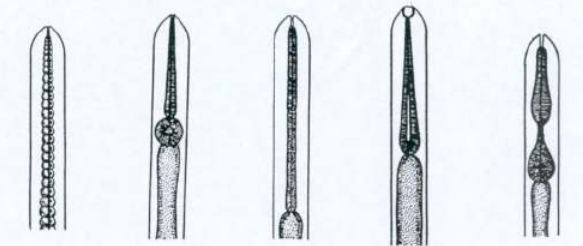
\includegraphics[width=0.8\columnwidth]{A.imagenes/ACV-BioSan-Parasit-NematodosMorf}
	\caption[Morfología de los esófagos de los nemátodos]{Tipos de esófagos de los nemátodos. De izquierda a derecha: tricuriforme, oxiuriforme, filariforme, estrogiloide y rhagditiforme.\label{fig:PARASIT:EsofagosMorf}}
\end{figure}
\subsubsection{\textit{larva migrans} cutanea}
Producida por nemátodos adaptados al ser humano (\textit{Ancylostoma braziliensis}, \textit{A. caninum}, \textit{A. plebotonum}), larvas que se pierden pese a estar adaptadas; y miasis del género \textit{Hypoderma} (ganado vacuno) o \textit{Gasterophilus} (ganado equino). Su diagnóstico es clínico basado en lesiones. Se pueden extraer para su análisis etiológico o mediante tiras para localizar inmunoglobulinas IgE. 
\newpage
\section{Superfamilia \textit{Filaroidea}}
\subsection{\textit{Wachereria bancrofti}}
\subsection{\textit{Dirofilaria inmitis}}
\newpage
\section{Otras familias}
\subsection{\textit{Trichuris trichuria}}
Nemátodo cosmopolita, suele predominar en climas templados y tropicales. Muy común en Asia y Centro y Sudamérica, sobre todo en Brasil. Además, suele coexistir con otros geohelmintos (\textit{Ascaris}, \textit{Enterobius}, etc.) y protozoos (\textit{Giardia}).
\subsubsection{Morfología}
La proción del cuerpo más fina se encuentra ocupada por un esófago tricuriforme, formado por células glandulares superpuestas denominadas esticocitos, formadores del esticosoma, al igual que \textit{Trichinella}.

La hembra es más rectilínea que el macho, que tiene la parte posterior en espiral, donde posee una espícula protegida por una vaina espicular. La hembra posee un ovario y un útero. Los huevos son en forma de huso o limón, con 2 tapones mucosos y en la puesta están sin embrionar. En el exterior se desarrolla la larva L1, que es el agente etiológico.
\begin{figure}[H]
	\centering
	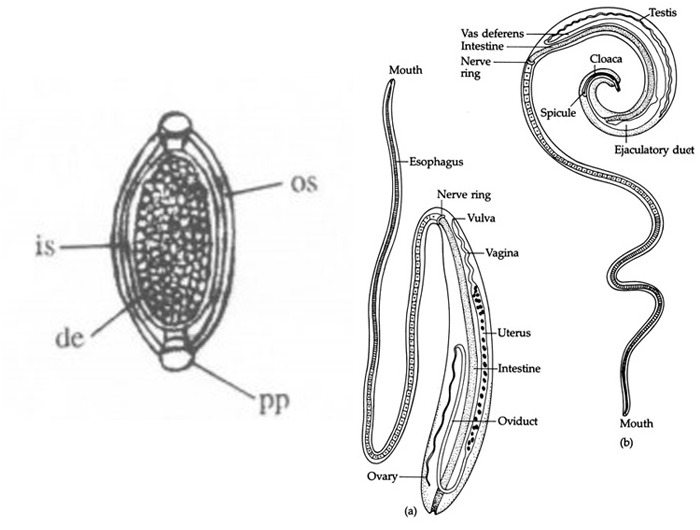
\includegraphics[width=0.6\columnwidth]{A.imagenes/ACV-BioSan-Parasit-TTrichuriaMorf}
	\caption[Morfología de \textit{T. trichuria}]{\textbf{Izquierda}: Huevo de \textit{T. trichuria}, \textbf{OS}: capa exterior; \textbf{IS}: caparazón interior; \textbf{DE}: embrión en desarrollo; \textbf{PP}: papilas polares. \textbf{Centro y derecha}: Fase adulta, \textbf{a)}, hembra; \textbf{b)}, macho \label{fig:PARASIT:TTrichuriaMorf}}
\end{figure}
\begin{multicols}{2}
	\subsubsection{Ciclo biológico}
	Mediante verduras o agua contaminadas con huevos con la larva L1. Los huevos pasan al intestino y en el duodeno se libera la larva L1, dirigiendose a la zona ileoceclar para producirse sucesivas mudas hasta la larva L4 y al fin el adulto, tardando unos 3 meses. En ese momento, machos y hembras copulan y la hembra comienza a eliminar los huevos a razón de 2000 a 20000 por día y hembra. Los huevos salen al exterior mediante las heces y tras unas 2 semanas a una temperatura mayor de 20 C y protegidos de la luz solar, se forma la larva L1, que vuelve a iniciar el ciclo.
	\subsubsection{Control}
	\begin{itemize}[itemsep=0pt,parsep=0pt,topsep=0pt,partopsep=0pt]
		\item Diagnóstico y tratamiento adecuado.
		\item Control de aguas, verduras. Eliminar el hábito de pica. Medidas de higiene
		\item Control de vectores mecánicos como moscas.
	\end{itemize}
	\columnbreak
	\begin{figure}[H]
		\centering
		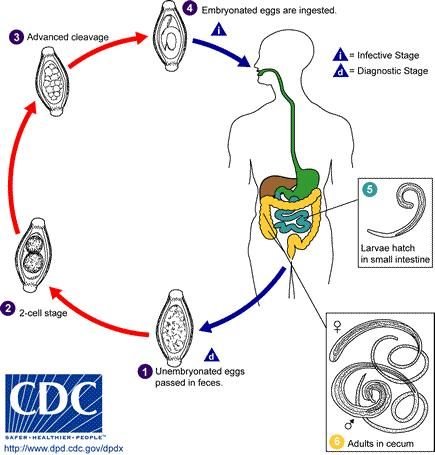
\includegraphics[width=0.95\columnwidth]{A.imagenes/ACV-BioSan-Parasit-TTrichuriaCBios}
		\caption[Ciclo biológico de \textit{T. trichuria}]{Ciclo biológico de \textit{T. trichuria}. Agente: Larva L1 \label{fig:PARASIT:TTrichuriaCBios}}
	\end{figure}
\end{multicols}
\subsubsection{Patogenia}
La tricuriasis tiene un periodo de incubación de 2 a 3 meses, un periodo prepatente de 3 meses y un periodo patente de varios años. Dependiendo de la dosis infectante, puede ser desde asintomática a mortal. Las acciones de \textit{T. trichuria} son:
\begin{itemize}[itemsep=0pt,parsep=0pt,topsep=0pt,partopsep=0pt]
	\item\textbf{Traumática}: en la mucosa, por la presencia de un estilete en la boca que clava en la mucosa y además secreta enzimas proteolíticas con inflamación de mucosa intestinal (llega al sangrado en infecciones masivas) e irritación de plexos nerviosos con hipermotilidad y diarrea.
	\item \textbf{Tóxica}: debido a las sustancias proteolíticas, lo cual se verá mediante la presencia de cristales de Charcot-Leyden en heces, resultado de una eosinofilia.
\end{itemize}
\subsubsection{Sintomatología}
Cursa con dolor abdominal, cefalea, hiperperistaltismo y disenteía y tenesmo. En infecciones masivas (sobre todo en niños), suele cursar con malnutrición que desemboca en anemias, generadas por la acción traumática del adulto que desemboca en malabsorción. La anemia se ve en dedos en palillos de tambor, retraso físico y mental y prolapso rectal.
\subsubsection{Diagnóstico}
\begin{itemize}[itemsep=0pt,parsep=0pt,topsep=0pt,partopsep=0pt]
	\item \textbf{Clínico y etiológico}: si existe prolapso, se pueden observar adultos. Si no, con una colonoscopia. También un síntoma son los dedos en palillos de tambor.
	\item \textbf{Etilológico}: mediante la visión en coprología de cristales de Charcot-Leyden y huevos, dependiendo del número de huevos, se puede ver la masividad de la infección.
\end{itemize}
\newpage
\subsection{\textit{Trichinella spiralis}}
\newpage
\subsection{\textit{Strongyloides stercolaris}}
\textit{Strogyloides stercolaris} es un parásito cosmopolita con alta prevalencia en zonas subtropicales (30 a 100 millones de infectados a nivel global). Son parásitos heterógonos, que alternan vida libre y parásita. Las hembras son partenogenicas\footnote{Hay una hipótesis para explicar la partenogénesis y es la reproducción protándrica: primero se desarrolla una gónada másculina para generar gametos, luego una femenina y se da la autofecundación.} y producen huevos transparentes, ovalados y con opérculo.
\subsubsection{Morfología}
\begin{itemize}[itemsep=0pt,parsep=0pt,topsep=0pt,partopsep=0pt]
	\item \textbf{Vida libre}: tienen una representación cromosómica haploide (machos) o diploide (hembras). Presentan un esófago rabditoide con una protursión prebulbo y una vulva dispuesta anteriormente. Las hembras de vida libre son más pequeñas y ponen más huevos que las parásitas, ya que poseen dos ovarios y dos úteros (frente al único ovario y útero de las parasitarias). Anfidelfas, un útero va a posterior (asociado a la puesta de huevos) y otro anterior. En el propio útero se desarrollan hasta la primera fase larvaria (L1). Posteriormente desarrollan un esófago rabdiforme y continuan su ciclo (L1r\footnote{r por su tipo de esófago, rabdiforme; frente a f, filariforme}, L2r, L3f, L4) fuera del útero.
	\item \textbf{Vida parásita}: presentan una dotación cromosómica triploide, en el caso de las hembras. Son también anfidelfas y presentan una esófago filariforme. Presentan un ciclo vital similar al anterior, pero sin fase L4.
\end{itemize}
\subsubsection{Ciclo biológico}
El ciclo vital puede ser:
\begin{itemize}[itemsep=0pt,parsep=0pt,topsep=0pt,partopsep=0pt]
	\item \textbf{Indirécto o heterogónico}: fases de vida libre.
	\item \textbf{Dirécto u homogónico}: en sus fases de vida parásita. El individuo avanza en su ciclo vital hasta la fase L3r y se produce una penetración al hospedador via subcutánea, transplacentaria, galactógena u oral.
\end{itemize}

Cuando la larva L3f penetra por la piel del hospedador definitivo, se desplaza por el sistema linfático y el torrente sanguíneo hasta las arterias pulmonares. Sigue avanzando hasta que rompe capilares y accede al espacio alveolar. Una vez allí, asciende por la tráquea hasta que es deglutida. En el intestino, la larva L3f se transforma en L4f y pasa a la adultez. Allí, tendrá lugar la partenogénesis y pondrá huevos saliendo la larva L1r en su interior. Los que tengan dotación cromosómica n o 2n, saldrán al exterior y seguirán un ciclo de vida indirecto o, en el caso de las larvas triploides, eclosionarán en el intestino, pudiendo:
\begin{itemize}[itemsep=0pt,parsep=0pt,topsep=0pt,partopsep=0pt]
	\item \textbf{Endoautoinvasión}: muda a L2r y a L3f y vuelve al torrente sanguíneo atravesando el intestino.
	\item \textbf{Migración a zona perianal}: se produce una muda a L2r y a L3f. Muchas de estas se caen del individuo contaminando el suelo permitiendo la infección de otros individuos (no humanos incluidos). Otras intentan penetrar por la piel (exoautoinvasión), en un fenómeno conocido como erupción reptante perianal. Los túneles subcutáneos son muy característicos, observándose un extremo vesiculoso que marca el avance de la larva, y el resto seco y duro. Remitirá a las dos o tres semanas. La larva L3f cerraría el ciclo.
\end{itemize}
\begin{multicols}{2}
	\begin{figure}[H]
		\centering
		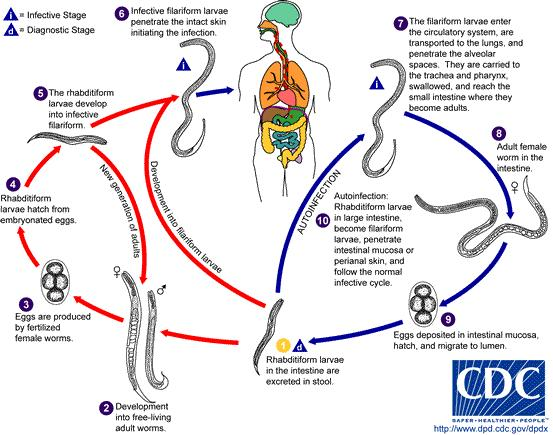
\includegraphics[width=0.9\columnwidth]{A.imagenes/ACV-BioSan-Parasit-SStercolarisCbios}
		\caption[Ciclo vital de \textit{S. stercolaris}]{Ciclo vital de \textit{S. stercolaris}. Agente: Larva L3f.\label{fig:PARASIT:SStercolarisCBios}}
	\end{figure}
	\begin{figure}[H]
		\centering
		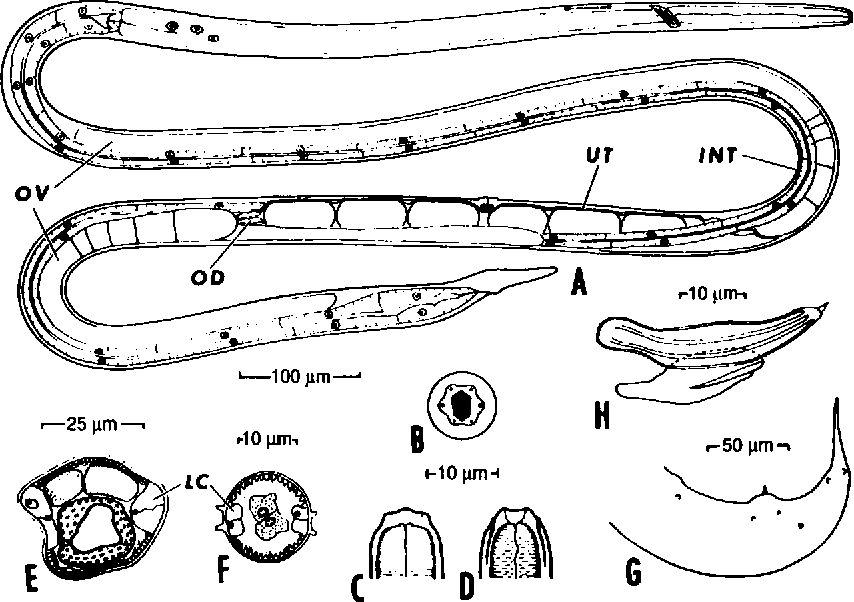
\includegraphics[width=0.9\columnwidth]{A.imagenes/ACV-BioSan-Parasit-SStercolarisMorf}
		\caption[Morfología de la forma parásita de \textit{S. stercolaris}]{Morfología de la forma parasitaria de \textit{S. stercolaris}. \textbf{A}: Visión lateral de una hembra parasitaria (OV: ovario, OD: oviducto, UT: útero, INT: intestino); \textbf{B}: vista anterior apical; \textbf{C}: Vista posterior lateral; \textbf{C}: Vista posterior dorsal; \textbf{E}: Sección a nivel del ovario (LC: cordón lateral); \textbf{F}: Sección intestinal de la larva filariforme; \textbf{G}: vistal de la cola de macho de vida libre; \textbf{H}: Espícula derecha bajo la línea del gobernáculo.\label{fig:PARASIT:SStercolarisMorf}}
	\end{figure}
\end{multicols}

\subsubsection{Patogenia}
El periodo de incubación es de unas dos semanas y el prepatente de 2 a 3 semanas.
\begin{itemize}[itemsep=0pt,parsep=0pt,topsep=0pt,partopsep=0pt]
	\item \textbf{Fase invasiva}: la larva L3f penetra por la piel. Se da una acción traumática y vehiculizadora de bacterias procedentes del interior (microbiota intestinal) o del exterior (suelo), generando hinchazón en el punto de la picadura, prurito local y \textit{larva migrans} cutánea.
	\item \textbf{Fase pulmonar}: acción traumática (ruptura de capilares) y vehiculadora. Causa hemorragias, síntomas asmáticos, tos seca e improductiva, dolor en el pecho, etc. que pasan desapercibidos salvo si se cursa una neumonía bacteriana.
	\item \textbf{Fase intestinal}: acción traumática de la L4f y de los adultos en las vellosidades. Producen un fuerte y punzante dolor epigástrico y diarreas que se exacerban con el consumo de corticoides con parasitaciones masivas.
\end{itemize}
\subsubsection{Diagnosis}
\begin{itemize}[itemsep=0pt,parsep=0pt,topsep=0pt,partopsep=0pt]
	\item \textbf{Etiológico}: en pequeñas infestaciones, mediante el método de concentración de Baermann, que concentra con hidro y termotropismo positivo a la larva y la deja flotando en una solución de ZnS$o_4$. Se ha visto que las hembras son capaces de producir huevos en alveolos pulmonares, por lo que se pueden ver en aspirados pulmonares hembras adultas, huevos y larvas L3f.
	\item \textbf{Indirecto}: muy útil en las primeras fases en las que el parásito se encuentra en la sangre. Mediante ELISA o IFI se pueden ver, pero producen reacciones cruzadas con los ancilostómidos.
\end{itemize}
\newpage
\subsection{\textit{Ancylostoma duodenale} y \textit{Necator americanus}}
\subsubsection{Morfología y localización}
\begin{multicols}{2}
	\subsubsection*{\textit{Ancylostoma duodenale}}
	\textit{Angylostoma duodenale} es una uncinaria del Viejo Mundo. Presenta una cápsula con dientes (4 superiores y dos en la base) con los que cortan las microvellosidades. Los machos son más pequeños que las hembras. En sus glándulas esofágicas presentan sustancias anticoagulantes que permiten la salida de sangre, lo que llevará el desarrollo de anemias por la pérdida de sangre. Las larvas son hematófogas y los adultos se alimentan de plasma, que llegan a obtener el 50 \% del hierro reducido perdido.
	
	Presentan un esófago estrongiliforme, muy musculoso, ligeramente más ensanchado en posterior. Las hembras son anfidelfas y ovíparas, liberan sus huevos en estado de mórula. Los machos presentan bolsa copuladora con tres lóbulos y costillas laterales separadas. Las espículas también están separadas. La larva L3 posee una punta muy puntiaguda y madura a 22 grados.
	\columnbreak
	\subsubsection*{\textit{Necator americanus}}
	\textit{Necator americanus} es la uncinaria del Nuevo Mundo. Posee una cápsula con 2 placas cortantes en la parte superior y dos dientes en la parte inferior.  Al igual que los \textit{Ancylostomas}, los machos son más pequeños que las hembras (anfidelfas y ovíparas, que eliminan huevos en forma de mórula), y poseen esófagos estrongiloides con glándulas secretoras de anticuagulantes.
	
	Los machos poseen bolsas copuladoras  con tres lóbulos y costillas laterlaes semifusionadas. Las espículas se fusionan en la punta y la larva L3 termina en punta roma. Mudan a 28 - 32 grados.
\end{multicols}
\vspace*{-1cm}
\begin{figure}[H]
	\centering
	\subfigure[Morfología de \textit{A. duodenale}]{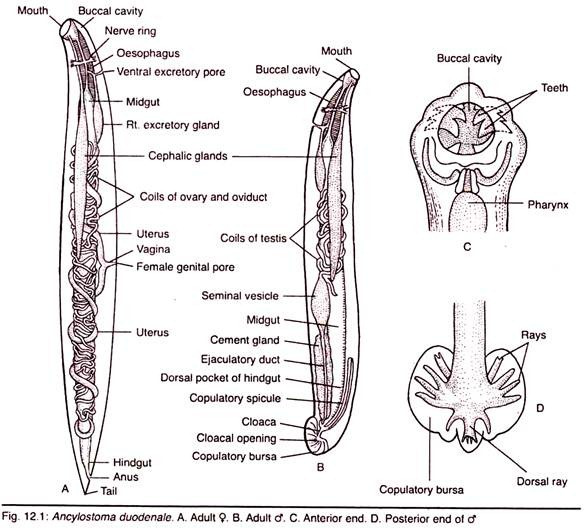
\includegraphics[width=0.475\columnwidth]{A.imagenes/ACV-BioSan-ParasitAduodenaleMorf}}
	\subfigure[Diferencias morfológicas entre \textit{A. duodenale} y \textit{N. americanus}]{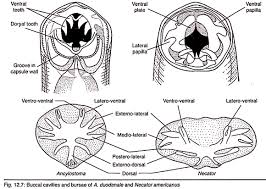
\includegraphics[width=0.475\columnwidth]{A.imagenes/ACV-BioSan-ParasitAduodenaleNamericanusMorf}}
	\caption[Morfología de \textit{A. duodenale} y \textit{N. americanus}]{Morfología de \textit{A. duodenale} y \textit{N. americanus} y sus diferencias más notables.}
\end{figure}
\subsubsection{Ciclo biológico}
La vía de infección es percutánea, aunque \textit{Ancylostoma duodenale} pueden infectar por vía oral, transplacentaria o galactógena.

El ciclo comienza con las larvas L3, que mediante su geotropismo negativo y fototropismo y termotropismo positivos, localizan un animal y penetran por la piel de zonas de los pies, al disponerse como agujas en posición vertical. En este contexto, alguna larvas L3 se pierden por la piel y forman el síndrome de la \textit{larva migrans} subcutánea. Una vez en el organismo, la larva L3 viaja por el sistema circulatorio hasta el corazón y las arterias pulmonares para salir por ellos y ser deglutidos al subir por la faringe. Una vez deglutidas, la larva L3 muda a L4 a los 5 días y a adulto a las 8 semanas. En ese momento se da la reproducción, expulsandose los huevos embrionados en forma de mórula. Tras 7 días, eclosiona la larva L1, que muda en el exterior a L2 y L3. Así mismo, \textit{A. duodenale} es capaz de quedarse latente en distintos tejidos e infectar mediante huevos embrionados o ingestión de larva L3.

Tiene como reservorios el cerdo, los perros y las vacas.
\begin{figure}[H]
	\centering
	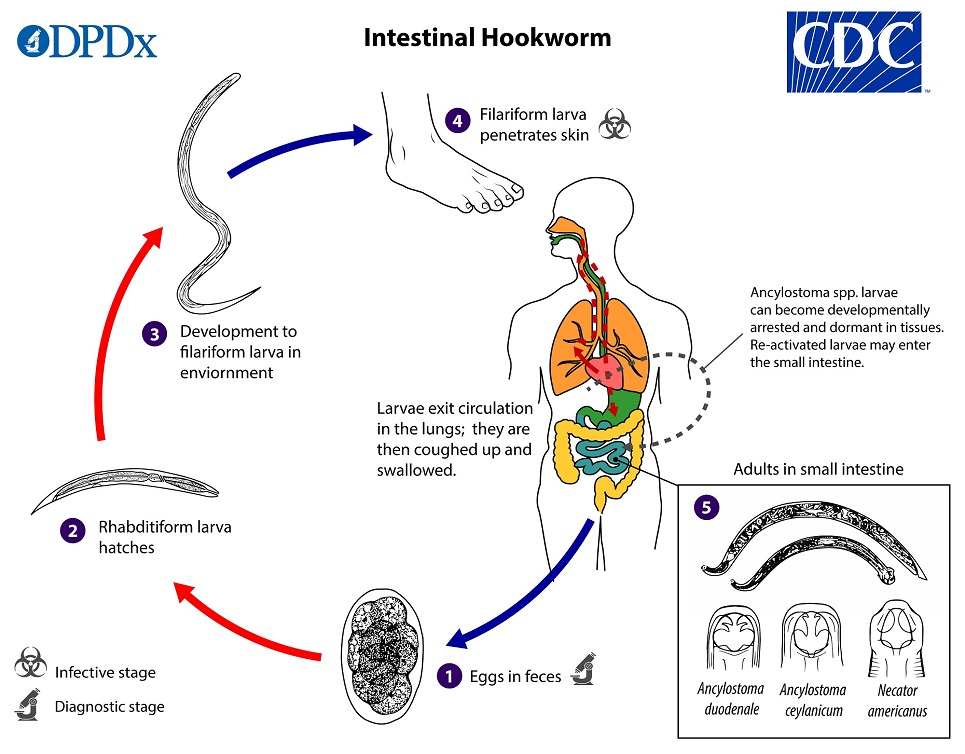
\includegraphics[width=0.7\columnwidth]{A.imagenes/ACV-BioSan-ParasitAduodenaleNamericanusCBios}
	\caption[Ciclo vital de \textit{A. duodenale} y \textit{N. americanus}]{Ciclo vital de \textit{A. duodenale} y \textit{N. americanus}. Agente: Larva L3f.\label{fig:PARASIT:AduodenaleNamericanusCBios}}
\end{figure}
\subsubsection{Patogenia y sintomatología}
La uncinariosis, su gravedad, depende, del número de parásitos, la duración del periodo patente (antes de aplicar tratamientos) y el estado nutricional, fisiológico e inmunológico del infectado. El periodo de incubación es de 4 horas, el prepatente de 5 a 6 semanas y el patente de hasta 20 años. Las uncinarias segregan distitnas moléculas que inhiben o antagonizan con la respuesta inmune. En cuanto a síntomas y daños:
\begin{itemize}[itemsep=0pt,parsep=0pt,topsep=0pt,partopsep=0pt]
	\item\textbf{Fase invasiva}: se produce urticaria y adenopatías en los ganglios cercanos, que siguen presentes durante toda la enfermedad. La inflamación ganglionar es indolora y los gánglios, móviles.
	\item\textbf{Fase pulmonar}: si la parasitosis es masiva, por la acción vehiculizadora pueden producir neumonías y pequeñas hemorragias. Generan una eosinofilia importante. Generan tos seca e improductiva.
	\item\textbf{Fase intestinal}: la larva L3 se alimenta de sangre, se reabsorben el 50 \% del hierro que estas toman. Las infecciones tienden a la cronificación y llevar a anemias. Los niveles de albúmina descienden a valores mínimos con resecación de piel y pelo. El dolor abdominal es insidioso, intermitente y ligero. Puede producirse anorexia y deposiciones con sangre. En niños puede provocar retraso mental y retardo en la pubertad.
\end{itemize}
\subsubsection{Diagnóstico}
\begin{itemize}[itemsep=0pt,parsep=0pt,topsep=0pt,partopsep=0pt]
	\item\textbf{Etiológico} mediante coprología se pueden ver huevos ovalados, transparentes y sin larvas en su interior.
\end{itemize}
\newpage
\subsection{\textit{Ascaris lumbricoides}}
Nemátodo cosmopolita, con mayor frecuencias en zonas tropicales y templadas. Tiene prevalencias mundiales de unos 1000 millones de personas, con unas 20 mil muertes anuales. Fue uno de los primeros parásitos en conocerse, debido a su enorme tamaño: los machos rondan los 15 a 30 cm y las hembras de 20 a 40.
\subsubsection{Morfología}
Machos y hembras poseen una boca con tres grandes labios, los cuales están rodeados de dentículos que, en \textit{A. lumbricoides} son cónicos, pero que en \textit{A. suum}\footnote{Parásitos de cerdos} son aplanados. Su esófago es estrongiliforme o en forma de mazo. Los machos no tiene bolsa copuladora, pero sí dos espículas iguales y anchas con las que penetra en la vulva y facilita la cópula. Poseen numerosas papilas anales y postanales. Las hembras presentan la vulva en el tercio anterior del cuerpo, 2 ovarios y 2 úteros enrollados sobre el intestino, los cuales pueden contener hasta 27 millones de huevos.

Los huevos son de color amarillo-marrón y son muy resistentes a los ácidos gracias a tres capas: una externa albuminoide (en pegotes); una media quitinosa y una intern lipídica, la cual le confiere una gran resistencia. Si el huevo está sin embrionar es de forma más alargada y estrecha, y si está embrionado (que son los que elimina la hembra) es redondo. El agente etiológico es el huevo con la larva L3 en su interior.
\subsubsection{Ciclo biológico}
Comienza con la ingestión de alimentos, agua o tierra contaminados con huevos con L3. Atraviesan el estómago y en el duodeno eclosionan, liberando a la L3, que atraviesa la mucosa intestinal y pasa a un capilar sanguineo, mediante el cual llega a la aorta y de ahí a los pulmones. rompiendo los capilares pulmonares, sale al espacio alveolar y ahí provoca que L3 suba por la tráquea para ser deglutida, volviendo al intestino. Allí, se transforma en L4 y en adulto. En unos 20 días tras la ingestión, las larvas L3 están en el pulmón, en unos 30 se transforman en adultos y en 2 meses eliminan huevos, que tras dos semanas a temperaturas templadas y en oscuridad, se transforman en L3.
\subsubsection{Control}
\begin{itemize}[itemsep=0pt,parsep=0pt,topsep=0pt,partopsep=0pt]
	\item Correcto saneamiento de las aguas, control de las heces y buenas prácticas higiénicas.
	\item Correcto diagnóstico y tratamiento en personas parasitadas.
\end{itemize}
\begin{multicols}{2}
	\begin{figure}[H]
		\centering
		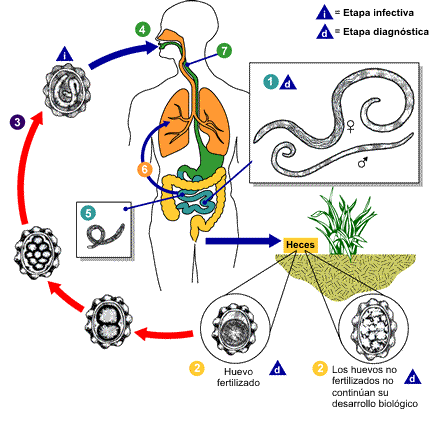
\includegraphics[width=0.9\columnwidth]{A.imagenes/ACV-BioSan-Parasit-ALumbricoidesCBios}
		\caption[Ciclo vital de \textit{A. lumbricoides}]{Ciclo vital de \textit{A. lumbricoides}. Agente: Larva L3f.\label{fig:PARASIT:AlumbricoidesCBios}}
	\end{figure}
	\columnbreak
	\begin{figure}[H]
		\centering
		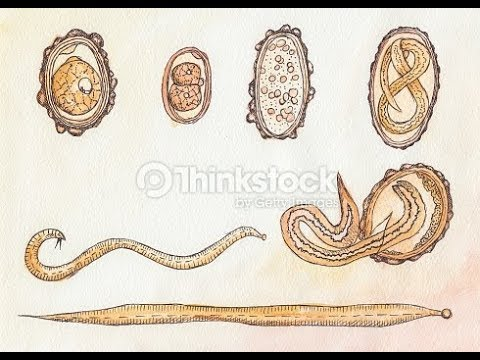
\includegraphics[trim=0 0.5cm 0 0.5cm,clip,width=\columnwidth]{A.imagenes/ACV-BioSan-Parasit-ALumbricoidesMorf}
		\caption[Morfología de \textit{A. lumbricoides}]{Morfología de \textit{A. lumbricoides}. En la parte superior, las diferente fases del huevo hasta la formación de la larva L1; en la parte media, un macho y el momento de la salida de la larva L1 del huevo; parte inferior, una hembra.\label{fig:PARASIT:AlumbricoidesMorf}}
	\end{figure}
\end{multicols}
\subsubsection{Patogenia}
La ascariasis produce las siguientes acciones:
\begin{itemize}[itemsep=0pt,parsep=0pt,topsep=0pt,partopsep=0pt]
	\item\textbf{Traumática}: por parte de la larva L3 por la ruptura de capilares pulmonares. Cuando la infección es masiva y se presenta con fiebre, ésta provoca la movilización de los adultos, que intentan escapar por los orificios del cuerpo, normalmente ano, pero también nariz, ojo, oído o boca, produciéndose acciones traumáticas.
	\item\textbf{Vehiculadora}: de larva L3 mediante el transporte de bacterias del intestino al pulmón.
	\item\textbf{Mecánica}: de obstrucción de los adultos en el intestino.
	\item\textbf{Expolidora y tóxica}: por parte de los adultos.
\end{itemize}
\subsubsection{Sintomatología}
El periodo de incubación es variable y depende del grado de parasitación desde 7 días en infestaciones masivas con síntomas pulmonares a 2 meses cuando hay problemas intestinales. El periodo prepatente es de 60 días y el patente puede extenderse durante años.

Las larvas producen inflamaciones por acción vehiculizadora, hemorragias en pulmón y edema. Con infecciones secundarias, se producen infiltrados de células epiteliales y glóbulos blancos y neumonía conocidos como síndrome de Loëfler que puede llevar a la muerte. Los adultos en el intestino producen enteritis (dolores intestinales), desnutrición y malabsorción de lactosa con pérdida apetito y peso, obstrucción intestinal y de conductos de glándulas anejas, fenómenos de sensibilización (prurito, urticaria, edema facial, insomnio) y eosinofilia en sangre. Los adultos errantes producen una fuerte acción traumática en su recorrido por su tamaño.
\subsubsection{Diagnóstico}
\begin{itemize}[itemsep=0pt,parsep=0pt,topsep=0pt,partopsep=0pt]
	\item\textbf{Etiológico}: por coprología, observando huevos a los dos meses de la infección, u observando larvas L3 en esputos o lavados gástricos.
	\item \textbf{Clínico}: por radiografía con la que se pueden ver las infecciones de un solo sexo.
	\item \textbf{Indirecto}: ELISA, RIA,$\dots$ en los periodos prepatentes (existen larvas L3 en sangre y producen una gran estimulación antigénica).
\end{itemize}
\newpage
\subsection{\textit{Enterobius vermicularis}}
Nemátodo parásito cosmopolita, predomina más en climas templados que en tropicales y aunque tiene una gama amplia de hospedadores definitivos, no se encuentra en perros o gatos. La incidencia en España es de unos 250 casos diagnosticados al año, no siendo cifras reales.
\subsubsection{Morfología}
Machos y hembras tienen el esófago oxiuriforme (con un bulbo) y en la parte anterior alas cefálicas. Las hembras miden entre 8 y 13 mmm, poseen 2 ovarios con dos úteros y una cola muy larga y puntiaguda denominada alfiler. Los machos miden entre 2 y 5 mm, con cola curvada y alas caudales. No tienen bolsa copuladora pero sí una espícula y unas papilas pre y poscloacales. No tienen gobernáculo.

Los huevos son transparentes, con uno de los lados más aplanado. Son muy ligeros, por lo que pueden estar suspendidos en el aire unos 2 minutos. Gozan de gran resistencia, pueden permanecer latentes hasta dos meses y son inmunes a insecticidas caseros. Los huevos que pone la hembra están embrionados con la larva L1.
\begin{figure}[H]
	\centering
	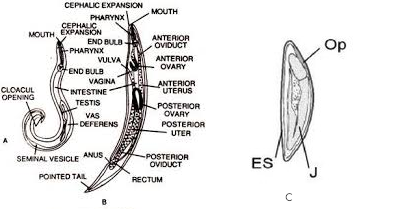
\includegraphics[width=0.8\columnwidth]{A.imagenes/ACV-BioSan-Parasit-EVermicularisMorf}
	\caption[Morfología de \textit{E. Vermicularis}]{Morfología de \textit{E. Vermicularis}.\textbf{A}: Macho; \textbf{B}: Hembra; \textbf{C}: Huevo, \textbf{OP}: opérculo, \textbf{ES}: capa externa, \textbf{J}: embrión \label{fig:PARASIT:EVermicularisMorf}}
\end{figure}
\vspace*{-1cm}
\subsubsection{Ciclo biológico}
\begin{multicols}{2}
	Comienza con la ingestión de alimentos o agua contaminados con huevos con la larva L2 o mediante inhalación y posterior deglución. En el intestino eclosiona el huevo, liberando la larva L2, que avanza por el intestino hasta la zona ileocecal, donde muda a larva L3, luego a larva L4 y posteriormente a adulto. Algunos adultos se alojan en el apéndice, por lo que pueden generar apendicitis. Machos y hembras copulan en la región ileocecal y se realiza la puesta de huevos tras dos mese. Los huevos no se eliminan por las heces, si no que al anochecer, la hembra viaja a los bordes perianales y pone allí los huevos. Si caen al exterior, necesitan un tiempo a una temperatura de 22 C para que mude la larva de L1 a L2. Si se quedan en la zona perianal, en unas 4 horas se produce la muda de L1 a L2. Las hembras, al movilizarse, provacan prurito anal, que al rascarse se quedan los huevos en las uñas y pueden llegar otra vez al intestino.
	\columnbreak
	\begin{figure}[H]
		\centering
		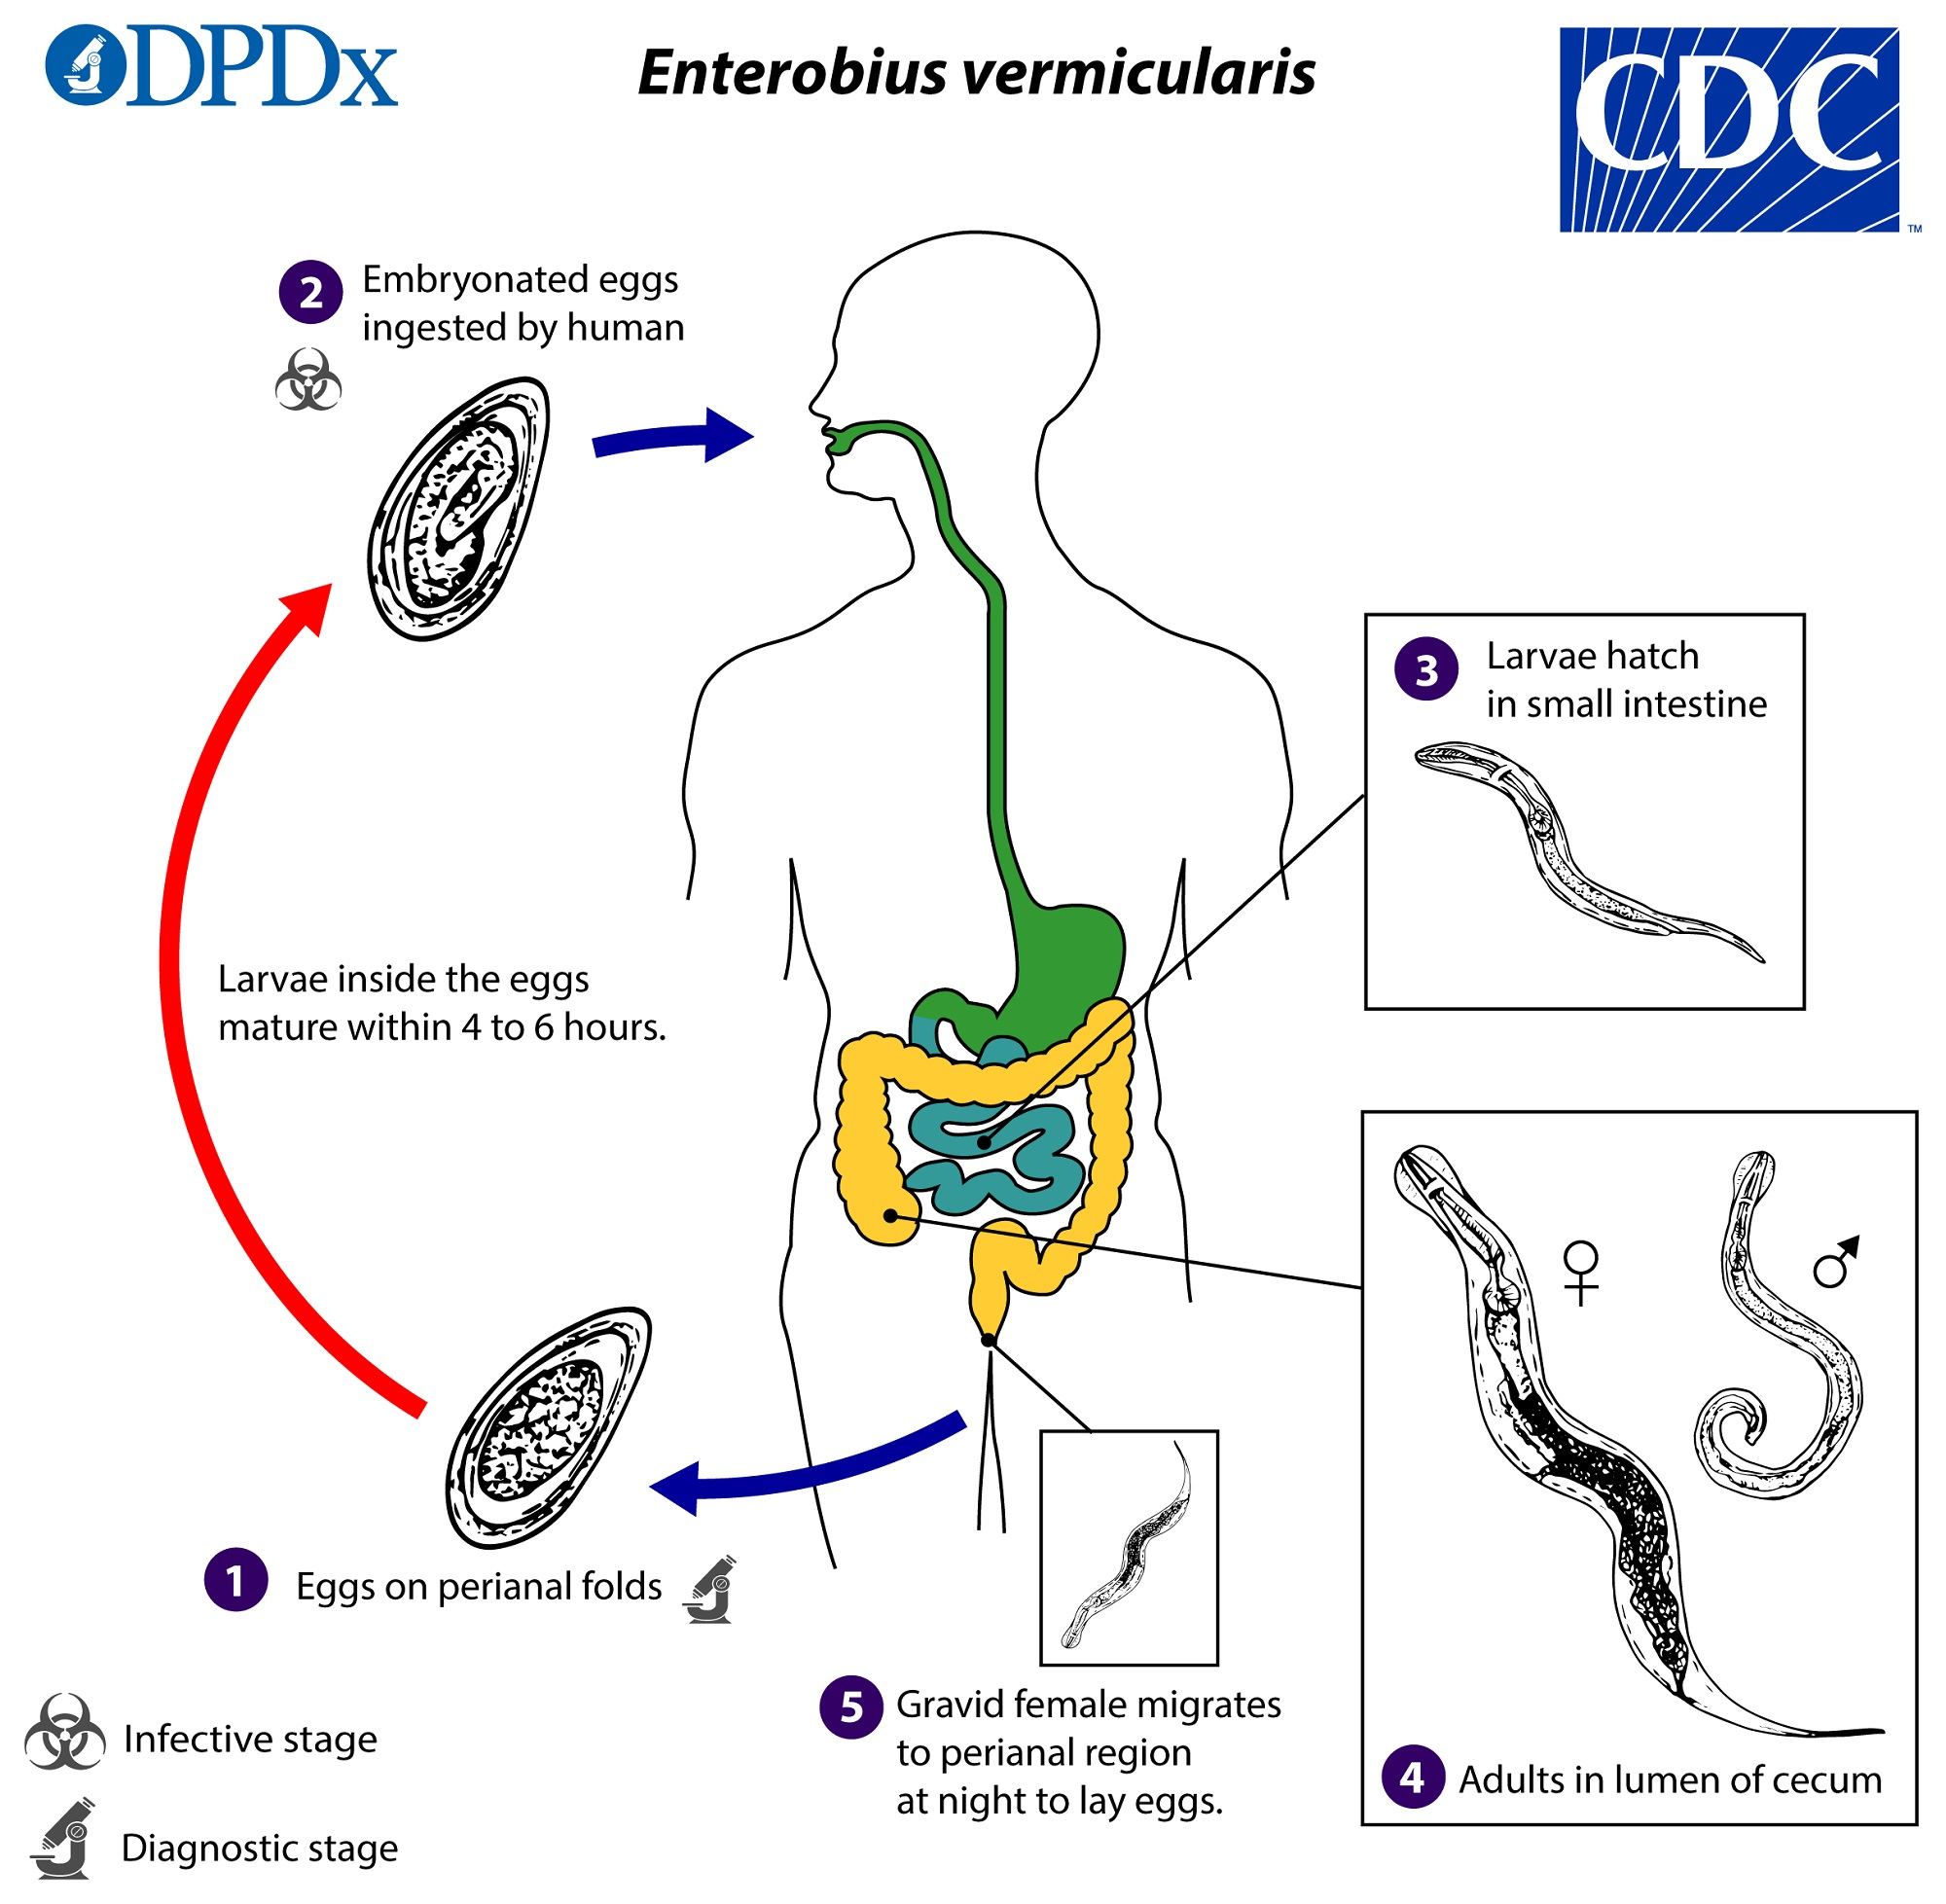
\includegraphics[width=\columnwidth]{A.imagenes/ACV-BioSan-Parasit-EVermicularisCBios}
		\caption[Ciclo vital de \textit{E. Vermicularis}]{Ciclo vital de \textit{E. Vermicularis}. Agente: Larva L2.\label{fig:PARASIT:EVermicularisCBios}}
	\end{figure}
\end{multicols}
Así, las vías de infección son:
\begin{itemize}[itemsep=0pt,parsep=0pt,topsep=0pt,partopsep=0pt]
	\item\textbf{Retroinfestación}: se produce cuando en la zona perianal eclosiona el huevo y la larva L2 vuelve por el ano al intestino, produciendose las mudas hasta llegar a la madurez.
	\item\textbf{Autoinfestación exógena}: mediante via ano-mano-boca.
	\item\textbf{Inhalación}: mediante el movimiento de objetos (sabanas, etc.) con huevos.
	\item\textbf{Ingestión}: por mala higiene y consumo de alimentos contaminados.
\end{itemize}
\subsubsection{Control}
El control se debe hacer a nivel de huevos, pues en cuanto hay un miembro de la familia parasitado, es muy fácil su contagio al resto. Se debe hacer analisis coprológico, tener cuidado al limpiar objetos, buenos hábitos de higiene.
\subsubsection{Patogenia}
La oxiurosis o enterobiosis es una enfermedad muy leve, no se detectan lesiones macroscópicas en el intestino. Sólo ejerce dos acciones: una tóxica que se manifiesta en forma de prurito nasal así como anal y vulvar por el movimiento de la hembra; y una acción vehiculizadora, dando lugar a vaginits con leucorrea o apendicitis.
\subsubsection{Sintomatología}
Cursa con prurito anal, vulvar y nasal, nerviosismos, bruxismo e insomnio.
\subsubsection{Diagnóstico}
Únicamente por diagnóstico etiológico (coprología). No solo se debe hacer de heces, pues solo se ven huevos si las heces arrastran los huevos de la región perianal. La mejor técnica es la de Graham o papel de celofán: se usa un portaobjetos con superficie adherente que se pasa por la zona perianal, donde se quedan pegados los huevos, se cubre con un cubreobjetos y se visualiza al microscopio. Si se sospecha de que hay una enterobiosis y da negativo, repetir la prueba a los pocos días sin que se produzca  limpieza en la zona que los elimine.
\newpage
\subsection{Anisakis}
    % SEC V - Artropodos
     \chapter{\textit{Phylum Arthropoda}}
\section{Orden \textit{Anaplura}}
\subsection{\textit{Pediculus humanus}}
\subsection{\textit{Phtirius pubis}}
\section{Orden \textit{Siphonaptera}}
\subsection{\textit{Ctenofephlidus canis}}
\subsection{\textit{Pulex irritans}}
\section{Orden \textit{Diptera}}
\subsection{\textit{Anopheles} spp}
\subsection{\textit{Aedes} spp}
\subsection{\textit{Cules} spp}
\subsection{Suborden \textit{Cyclorrhopla}} %Stomxys, Musca, Colliplora, Callitroga, Sarcophaga, Gastrophilus, Hypoderma, Oestres
\section{Clase \textit{Arachnida}}
\subsection{\textit{Rhipicephtlus variablis}}
\subsection{\textit{Argus persicus}}
\section{Miasis}
\subsection{dermatobia}
\subsection{Wolfartia}
\subsection{Lucilia}
    \part{Zoología}
     \chapter{Anatomía Animal comparada}
\section{Elementos de morfología}
\subsection{Simetría}
\paragraph{Morfología}: Ciencia auxiliar cuyo objeto es el estudio son los animales desde el punto de vista geométrico.
\paragraph{Ejes}: Línea imaginaria que atraviesa al animal de forma que todos sus elementos se encuentran en torno a ella. Se pueden diferenciar:
\begin{itemize}[itemsep=0pt,parsep=0pt,topsep=0pt,partopsep=0pt]
    \item \textbf{Eje oral-aborall}: desde la boca hasta el ano.
    \item\textbf{Eje apical-antiapical}: desde el extremo superior al inferior
\end{itemize}
\paragraph{Plano}: plano que corta al animal en dos imágenes especulares:
\begin{itemize}[itemsep=0pt,parsep=0pt,topsep=0pt,partopsep=0pt]
    \item \textbf{Sagital}: divide al animal en una parte izquierda y otra derecha.
    \item\textbf{Frontal}: divide al animal en una parte dorsal y otra ventral.
    \item\textbf{Transversal}: divide al animal en una parte anterior y otra posterior.
\end{itemize}
\begin{figure}[H]
    \centering
    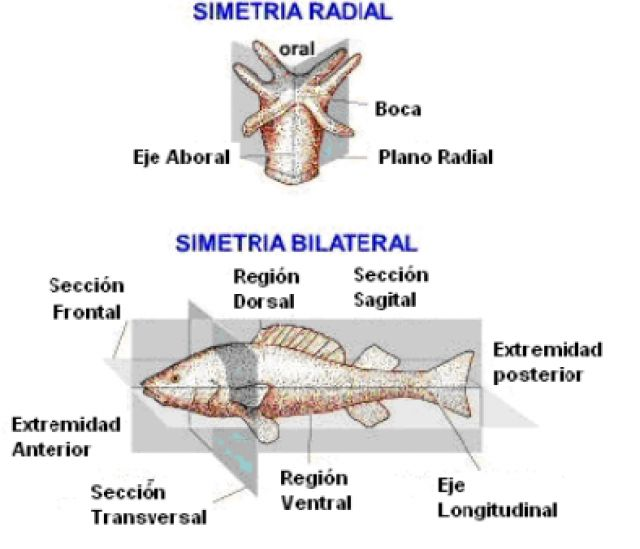
\includegraphics[width=0.65\columnwidth]{A.imagenes/ACV-ANATANIM-EjesPlanos}
    \caption[Ejemplos de Ejes y planos de simetría]{Ejemplos de Ejes y planos de simetría, en animales de simetría radial y de simetría bilateral.}
\end{figure}
\subsection{Clasificación morfológica}
\begin{itemize}[itemsep=0pt,parsep=0pt,topsep=0pt,partopsep=0pt]
    \item \textbf{Anoxonía}: No tienen ejes ni planos de simetría. Son organismos simples (amebas o poríferos), sésiles y poco evolucionados. Los individuos de la misma especie no son siempre iguales.
    \item\textbf{Homoaxonía}: son múltiples (infinitos) ejes homopolares e infinitos planos. Son organismos no animales (radiolarios, protozoos), esféricos.
    \item\textbf{Monoaxonía}: gran mayoría de animales, solo poseer un eje de simetría. Se dividen según planos en:
    \begin{itemize}[itemsep=0pt,parsep=0pt,topsep=0pt,partopsep=0pt]
        \item \textbf{Simetría radial}: infinitos planos de simetría un único eje. Son organismos simples, sésiles o poco móviles, habitan en el fondo marino.
        \item\textbf{Simetría birradial}: un eje de simetría y dos planos simétricos. Son organismos simples, śesiles o poco móviles, como los \textit{Cnidaria},$\dots$
        \item\textbf{Simetría pentaradial}: un eje de simetría y cinco planos de simetría (las partes del animal se repiten cinco veces. Propio de los equinodermos.
        \item\textbf{Simetría bilateral}: lo tienen gran cantidad de animales. Tienen una cabez (contiene centros nerviosos y se encuentran órganos de los sentidos). Son organismos complejos y con plano de simetría sagital. Determina la dirección del desplazamiento. Se distinguen dos regiones, por la cefalización:
        \begin{itemize}[itemsep=0pt,parsep=0pt,topsep=0pt,partopsep=0pt]
            \item \textbf{Cefálica}: contiene la zona oral y la cabeza y es la parte anterior.
            \item\textbf{Caudal}: contiene el resto del organismo del animal no incluida en la zona cefálica. Es la parte posterior.
        \end{itemize}
    \end{itemize}
    \item\textbf{Asimetrías}: alteraciones a la simetría:
    \begin{itemize}[itemsep=0pt,parsep=0pt,topsep=0pt,partopsep=0pt]
        \item \textbf{Organización interna}: el animal tiene órganos impares, diferenciandose dos partes desiguales internas.
        \item\textbf{Por uso}: el animal da preferencia al uso de una parte de su cuerpo en detrimento de su homóloga en la otra sección para una determinada acción (como zurdo$\leftrightarrows$diestro). Deriva de una laterización.
        \item\textbf{Ofensivo-Defensivo}: Una parte se ve más desarrollada que su homóloga, sirviendo al animal, para atacar o defenderse (por ejemplo, el cangrejo violinista).
        \item\textbf{Prefijado}: el animal hipertrofia una parte de su cuerpo (Narval, que desarrolla un colmillo para compensar a otro).
        \item\textbf{Por desarrollo}: el animal cambia o desarrolla una asimetría que se completa en la edad adulta (ej. osteictios pleuronectiformes).
        \item\textbf{Dobles simetrías}: animales segmentados.
        \item\textbf{Clinasimetría}: en un hemisferio y en otro tiene diferentes simetrías (ej. cnidarios en colonias, como el género \textit{Velella}).
    \end{itemize}
\end{itemize}
\subsection{Estructuras morfológicas}
\paragraph{Proglótides}: propia de los platelmintos (Cestodos). Se trata de un órgano sexual, sección de un estróbilo y no imprescindible. Es hermafrodita. Aumenta su grado de maduración con el alejamiento del escolex. Tienen tres fases:
\begin{enumerate}[itemsep=0pt,parsep=0pt,topsep=0pt,partopsep=0pt]
    \item Órgano sexual masculino.
    \item Órgano sexual femenino.
    \item Huevos (ruptura del proglótide y salen al exterior).
\end{enumerate}
\paragraph{Metámeros}: se da en los anélidos. El cuerpo se encuentra segmentado en anillos, imprescindibles (no se segmentan) y no regenerables. Cada sección contiene un vaso sanguineo dorsal y otro ventral, metanefridios (parte excretor, en la parte ventral), un cordón nervioso y una sección del tubo digestivo.
\begin{figure}[H]
    \centering
    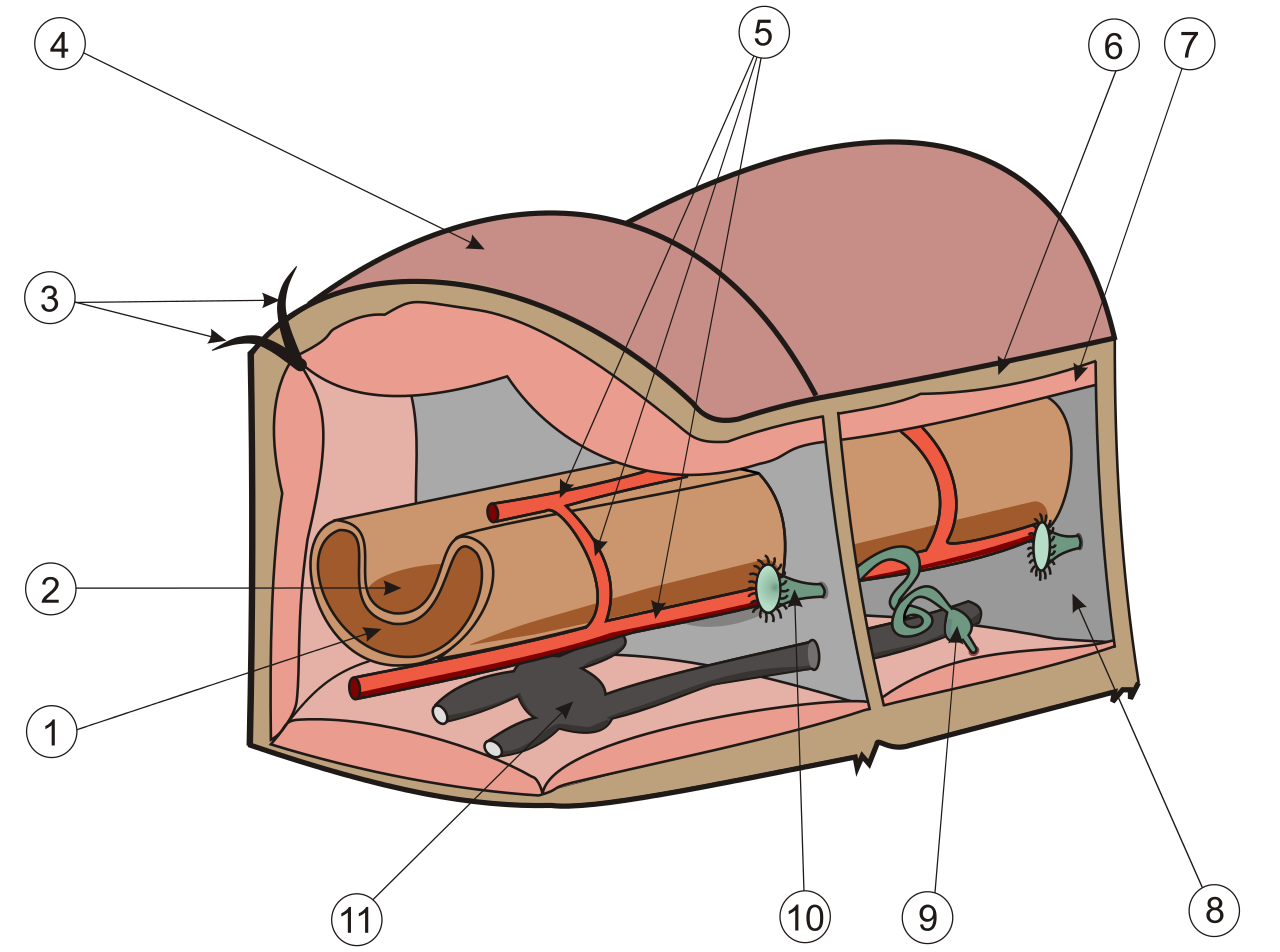
\includegraphics[width=0.5\columnwidth]{A.imagenes/ACV-ANATANIM-Metameros}
    \caption[Anatomía de un metámero]{Anatomía de un metámero: 1 - Lumen intestinal, 2 - Tiflosolio, 3 - Quetas, 4 - Cutícula, 5 - Vasos sanguíneos, 6 - Epitelio, 7 - Musculatura circular, 8 - Tabique del metámero, 9 - Célula terminal del metanefridio, conectando con el canal del metanefridio, 10 - Metanefridio, 11 - Ganglio nervioso del metámero.}
\end{figure}
\paragraph{Ciclómero}: propio de equinodermos y animales con simetría radial. Parte repetida circularmente, con los mismos órganos y estructuras (pueden regenerarse). Animales no cefalizados, cada brazo o sección tiene un tubo digestivo independiente, unas gónadas, un fotorreceptor y un sistema nervioso.
\paragraph{Tagma}: característico de artrópodos. Se da la unión de partes dedicadas a una misma función. Cada parte es la unión de metámeros dedicados a realizar una función, formando una unidad superior.  Se pueden distinguir un tagma cefálico (prostomeo y parte de un metámero), tagma torácico (función de movimiento de los metámeros y tubo digestivo), y tagma abdominal (reproducción).
\subsection{Clasificación del tipo de vida}
\begin{itemize}[itemsep=0pt,parsep=0pt,topsep=0pt,partopsep=0pt]
    \item Según su tipo de vida:
    \begin{itemize}[itemsep=0pt,parsep=0pt,topsep=0pt,partopsep=0pt]
        \item \textbf{Vida libre}: no viven pegados a otro ser.
        \item\textbf{Parásito}: vive fijado a un huésped. Si es en el exterior, se denomina ectoparásito; si está en el interior del ser vivo, es un endoparásito.
    \end{itemize}
    \item Según el medio que habitan:
    \begin{itemize}[itemsep=0pt,parsep=0pt,topsep=0pt,partopsep=0pt]
        \item \textbf{Terrestres}: viven sobre la superficie terrestre. Pueden ser epígeos (viven sobre la capa del suelo) o hipógeos (viven enterrados en la capa del suelo).
        \item\textbf{Acuáticos}: viven en la hidrosfera. Son dulceauicolas (viven en medios fluviales) o marinos (viven en el mar).
    \end{itemize}
    \item Seres acuáticos:
    \begin{itemize}[itemsep=0pt,parsep=0pt,topsep=0pt,partopsep=0pt]
        \item \textbf{Holobiontes}: el animal vive siempre en el mismo medio. Pueden ser talasobiontes (viven en el mar) o potamobiontes (viven en rios).
        \item\textbf{Anfiobiontes}: el animal vive una parte de su desarrollo en el mar o en rio y otra en el medio contrario. Según donde desovan son talasotocos (lo hacen en el mar), o potamotocos (lo hacen en el río).
    \end{itemize}
    \item Seres marinos:
    \begin{itemize}[itemsep=0pt,parsep=0pt,topsep=0pt,partopsep=0pt]
        \item \textbf{Bentónicos}: viven en el lecho marino (sésiles o poco móviles)
        \item\textbf{Pelágicos}: viven entre el fonto y la superficie marina (organismos nadadores).
        \item\textbf{Planctónicos}: viven en la superficie marina (arrastrados por la corriente).
    \end{itemize}
    \item Seres según su movilidad:
    \begin{itemize}[itemsep=0pt,parsep=0pt,topsep=0pt,partopsep=0pt]
        \item\textbf{Móvil}: se mueven.
        \item\textbf{Sécil} : se fijan al sustrato.
    \end{itemize}
    \item En relación a los comportamientos sociales:
    \begin{itemize}[itemsep=0pt,parsep=0pt,topsep=0pt,partopsep=0pt]
        \item \textbf{Solitarios}: no dependen unas de otros, viven en colonias ni tienen división de funciones.
        \item\textbf{Gregarios}: se reúnen en grupos con división de funciones.
        \item\textbf{Coloniales}: viven juntos y comparten partes del cuerpo.
    \end{itemize}
\end{itemize}
\section{Clasificación sistemática}
Se denomina \textbf{Taxonomía} a la ciencia auxiliar que ordena a los seres vivos con unas características comunes. Así mismo, una especie es la única categoría real, conjunto de seres vivos que se pueden reproducir entre si y que su descendencia sea fértil.
\section{\textit{Phylum Chordata}}
Los cordados tienen como características principales:
\begin{itemize}[itemsep=0pt,parsep=0pt,topsep=0pt,partopsep=0pt]
    \item \textbf{Epineuros}: tienen un tubo neural dorsal.
    \item\textbf{Faringotremados}: en algún momento de su desarrollo tienen una faringe perforada.
    \item\textbf{Cordados}: en algún momento de su vida tiene un esqueleto que es un filamento denominado corda. Es el soporte del cuerpo y eje esquelético donde se enganchan los músculos.
    \item En algún momento de su vida desarrollan una cola detrás del ano sin vísceras.
\end{itemize}
\subsection{Subfilo \textit{Tunichata} o Urocordados}
Subiertos por una capa (túnica). Sufren una metamorfosis drástica: de una cría con aspecto de renacuajo y con las características propias de los cordados, pasan a un adulo sin corda, tubo neural y cola. Se diferencian tres clases:
\begin{itemize}[itemsep=0pt,parsep=0pt,topsep=0pt,partopsep=0pt]
    \item \textbf{Ascideos}: tiene tres comportamientos sociales: sésiles, bentónicos y planctónicos.
    \item\textbf{Taliaceos}: son transparentes y planctónicos.
    \item\textbf{Apendicularios}: conservan todos los caracteres de los cordados.
\end{itemize}
\subsection{Subfilo \textit{Cephalochordata}}
También llamados anfioxos, tiene dos ejes y forma de huso. La corda les llega hasta la cabeza.
\subsection{Subfilo \textit{Vertebrata}}
Tienen el tubo neural tapado por vértebras. Se diferencian dos grupos principales:
\begin{itemize}[itemsep=0pt,parsep=0pt,topsep=0pt,partopsep=0pt]
    \item \textbf{Aganatos}: no tienen mandíbula, son:
    \begin{itemize}[itemsep=0pt,parsep=0pt,topsep=0pt,partopsep=0pt]
        \item \textbf{\textit{Myxines}}: saprófitos, al comer se enganchan al trozo a engullir, se anuda sobre sí mismos y al sacar la cabeza arrancan el alimento.
        \item\textbf{Lampreas}: ectoparásitos hematófogos, en la boca tienen una ventosa dentada, al igual que su lengua. Se agarra al huésped con la ventosa y este es perforado con la lengua.
    \end{itemize}
    \item\textbf{Gnatostomados}: tienen mandíbulas:
    \begin{itemize}[itemsep=0pt,parsep=0pt,topsep=0pt,partopsep=0pt]
        \item \textbf{Condríctios}: animales acuáticos, con branquias y esqueleto cartilaginoso. Anamniotas. Algunos representantes son las rayas o el tiburón.Se dividen en:
        \begin{itemize}[itemsep=0pt,parsep=0pt,topsep=0pt,partopsep=0pt]
            \item \textbf{Holocéfalos}: tienen un único agujero branquial. Se llaman, por su forma, \textit{quimeras monstruosas}.
            \item\textbf{Elasmobránquios}: tienen más de dos hendiduras branquiales.
        \end{itemize}
        \item\textbf{Osteíctios}: animales acuáticos con esqueleto óseo.Anamniotas. Se diferencian:
        \begin{itemize}[itemsep=0pt,parsep=0pt,topsep=0pt,partopsep=0pt]
            \item \textbf{Actinopterigios}: sólo tienen branquias.
            \item\textbf{Sarcopterígios}: tiene estructuras que darán lugar a pulmones.
        \end{itemize}
        \item\textbf{Anfibios}: animales de vida terrestre en hábitats húmedos.Anamniotas, de respiración pulmonar y cutánea. Necesitan un medio acuático o húmedo para reproducirse: los huevos se secarían. Las crias respiran bajo el agua.Se clasifican:
        \begin{itemize}[itemsep=0pt,parsep=0pt,topsep=0pt,partopsep=0pt]
            \item \textbf{Anuros}: sin cola.
            \item\textit{Urodelos}: con cola postanal sin vísceras.
        \end{itemize}
        \item\textbf{Reptiles}: animales de vida terrestre, amniotas y de respiración pulmonar. Se dividen según los agujeros craneales:
        \begin{itemize}[itemsep=0pt,parsep=0pt,topsep=0pt,partopsep=0pt]
            \item \textbf{Anápsidos}: no tienen agujeros craneales. (tortugas)
            \item\textbf{Diápsidos}: tienen dos agujeros en el cráneo , animales modernos . (serpientes).
            \item\textbf{Arcosaurios}: tienen dos agujeros en el cráneo, animales antiguos. (cocodrilos).
        \end{itemize}
        \item\textbf{Aves}: animales de vida terrestre, amniotas de respiración pulmonar. Tienen un cráneo derivado de un diápsido. Se pueden establecer:
        \begin{itemize}[itemsep=0pt,parsep=0pt,topsep=0pt,partopsep=0pt]
            \item \textbf{Ratites}: aves corredoras, no buceadoras ni voladoras, como el kiwi.
            \item\textbf{Impennes}: aves buceadoras, no corredoras ni voladoras, como el pingüino.
            \item\textbf{Carenados}: aves voladoras o que tienen estructuras preparadas para el vuelo.
        \end{itemize}
        \item\textbf{Mamíferos}: animales de vida terrestre, amniotas y de respiración pulmonar.
        \begin{itemize}[itemsep=0pt,parsep=0pt,topsep=0pt,partopsep=0pt]
            \item \textbf{Prototerios}: ponen huevos (ornitorrincos).
            \item\textbf{Terios}: no ponen huevos.
            \begin{itemize}[itemsep=0pt,parsep=0pt,topsep=0pt,partopsep=0pt]
                \item \textbf{Metaterios}: las crías nacen sin terminar de desarrollar, por lo que migran a una bolsa o marsupio donde terminan su desarrollo.
                \item\textbf{Euterios}: paren crías desarrolladas pero no siempre independientes.
            \end{itemize}
        \end{itemize}
    \end{itemize}
\end{itemize}
\begin{figure}[H]
    \centering
    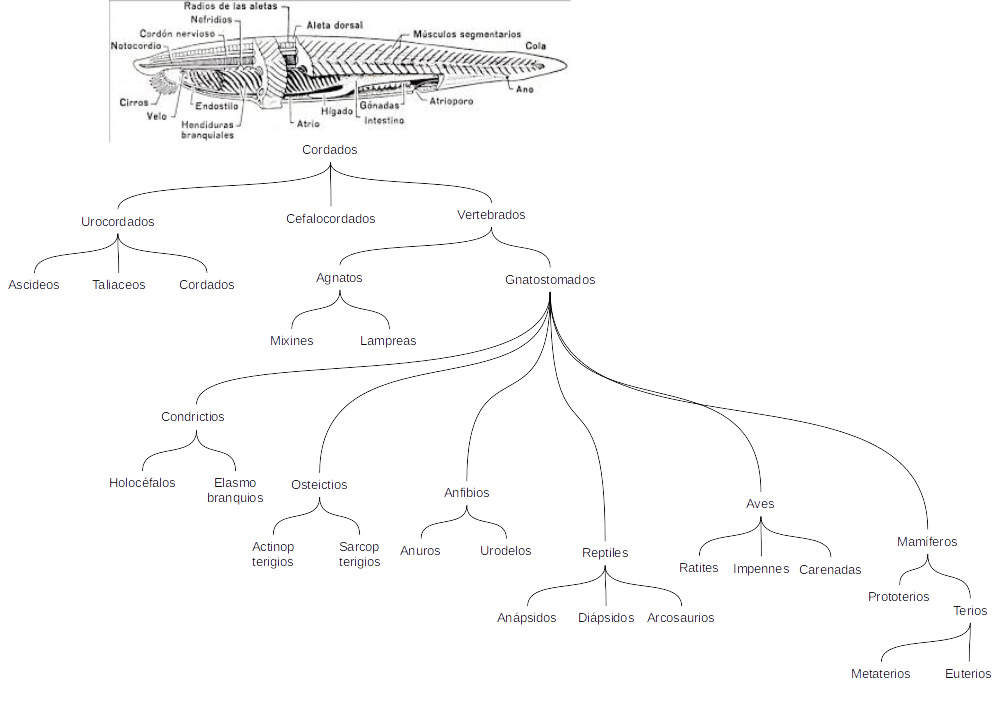
\includegraphics[width=\columnwidth]{A.imagenes/ACV-ANATANIM-Cordados}
    \caption{Clasificación y plan general de los cordados}
\end{figure}
\section{Desarrollo ontogenético}
Historia del desarrollo de un zigoto diplonte hasta que el individuo muere. Comprende:
\begin{itemize}[itemsep=0pt,parsep=0pt,topsep=0pt,partopsep=0pt]
    \item \textbf{Desarrollo embrionario}: observación de las distintas fases del zigoto. El desarrollo embrionario es algo exclusivo del reino \textit{Animalia}. Modos de reproducción:
    \begin{itemize}[itemsep=0pt,parsep=0pt,topsep=0pt,partopsep=0pt]
        \item \textbf{Reproducción asexual}: aquella en la que no hay meiosis, todos los individuos son clónicos.
        \item\textbf{Reproducción sexual}: aquella en la que hay meiosis. Es la única posible en los vertebrados. Se necesita un espermatozoide y un óvulo haploides formando un zigoto diploide. Puede ser mono o diparental, según intervengan uno o dos individuos.
    \end{itemize}
    \item\textbf{Desarrollo postembrionario}: paso del embrión al adulto y su posterior muerto.
\end{itemize}
\subsection{Zigoto: segmentación y gastrulación}
El zigoto es una célula resultante de la unión de dos gametos procedentes de dos gónadas distintas. Se distinguen por la distribución del vitelo, en cuatro tipos, que determinan la división celular.  Tras la formación del cigoto, llevará a cabo un proceso de segmentación, que es el conjunto de cariocinesis que lleva a cabo el zigoto para la formación de la gastrula. La gastrula es a su vez el proceso de invaginación del cigoto, formándose un blastoporo, orificio que comunica el exterior con el arquénteron (cavidad interna que dará lugar al endodermo).

Se pueden diferenciar cuatro tipos de zigoto:
\begin{itemize}[itemsep=0pt,parsep=0pt,topsep=0pt,partopsep=0pt]
    \item \textbf{Isolecito}: la materia nutritiva (vitelo) se reparte en pequeños gránulos uniformemente.
    \begin{itemize}[itemsep=0pt,parsep=0pt,topsep=0pt,partopsep=0pt]
        \item \textbf{Segmentación}: sufre una división igual y holoblástica (todos los blastómeros o células que forman la blástula, son iguales). El proceso consiste en sucesivos ciclos de mitosis iguales. En algunas especies, los blastómeros no son paralelos ni perpendiculares entre sí, si no que se desplazan uno respecto al otro, dando lugar a una diferenciación en segmentaciones radiales o espirales.
        \item\textbf{Gastrulación}: tanto las blástulas espirales como las radiales, las células de un polo sufren unas mitosis más acelaradas creando una región hueca, cuyo tapiz generará el endodermo, mientras que las células en el exterior dan lugar al ectodermo.
    \end{itemize}
    \item\textbf{Heterolocito}: el vitelo se reparte en gránulos pequeños en un polo animal y en gránulos grandes en polo vegetativo.
    \begin{itemize}[itemsep=0pt,parsep=0pt,topsep=0pt,partopsep=0pt]
        \item \textbf{Segmentación}: se dan dos subfases:
        \begin{itemize}[itemsep=0pt,parsep=0pt,topsep=0pt,partopsep=0pt]
            \item \textit{Hasta el cliclo segundo}: se tratan de divisiones holoblásticas e iguales resultando cuatro células (2 en el polo animal y dos en el polo vegetativo). Se diferencia así un polo vegetativo de crecimiento lento (por falta de vitelo) y un polo animal de crecimiento rápido.
            \item\textit{Hasta la blástula}: se da una división holoblástica desigual, pudiendo segmentarse radial o espiralmente. En cualquier caso, se crean dos tipos de células: micrómeros (blastómeros pequeños) y macrómeros (blastómeros grandes).
        \end{itemize}
        \item\textbf{Gastrulación}: En este caso, las células del endodermo son los macrómeros, de forma que el endodermo siempre lo forma el polo vegetativo.
    \end{itemize}
    \item\textbf{Telolecito}: vitelo gigante que rellena todo el cigote, dando un núcleo lateralizado.
    \begin{itemize}[itemsep=0pt,parsep=0pt,topsep=0pt,partopsep=0pt]
        \item \textbf{Segmetación}: Se dividen los nucleos en uno de los polos de la célula pero sin división citoplasmática. Tras un cierto número de ciclos, los núcleos forman protuberancias en la membrana, independizandose y generando un discoblasto. Los blastómeros irán consumiendo poco a poco el vitelo.
    \end{itemize}
    \item\textbf{Centrolecito}: vitelo gigante que rodea a un núcleo que se situa en el centro rodeado por vitelo.
    \begin{itemize}[itemsep=0pt,parsep=0pt,topsep=0pt,partopsep=0pt]
        \item \textbf{Segmetación}: En un primer paso, el nucleo migra a uno de los polos, dando lugar a un zigoto telolecito. Se dividen los nucleos en uno de los polos de la célula pero sin división citoplasmática. Tras un cierto número de ciclos, los núcleos forman protuberancias en la membrana, independizandose y generando un discoblasto. Los blastómeros irán consumiendo poco a poco el vitelo.
    \end{itemize}
\end{itemize}

El desarrollo embrionario puede continuar de dos formas:
\begin{itemize}[itemsep=0pt,parsep=0pt,topsep=0pt,partopsep=0pt]
    \item No se forma una tercera hoja embrionaria (animales diblásticos: Cnidarios y tenóferos). Estos animales desarrollan tejidos producidos por estas dos hojas: epidermis, sistema nervioso y tubo digestivo.
    \item Se forma una tercera hoja emprionaria (animales triblásticos). Apartir del endodermo, se forma una tercera hoja embrionaria o mesodermo. Se pueden diferenciar por dos procesos: esquizocelia y enterocelia. Según la formación del celoma, pueden ser: acelomados, pseudocelomados, celomados o enterocelomados.
\end{itemize}
\begin{figure}[H]
    \centering
    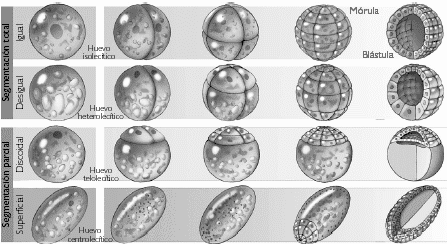
\includegraphics[width=0.8\columnwidth]{A.imagenes/ACV-ANATANIM-SegmetacionGastrulacion}
    \caption[Tipos de cigoto y modelos de segmentación]{Tipos de cigoto y modelos de segmentación. Primeras fases del desarrollo embrionario en los animales y tipos de segmentación según la cantidad y disposición del vitelo nutritivo.}
\end{figure}
\begin{figure}[H]
    \centering
    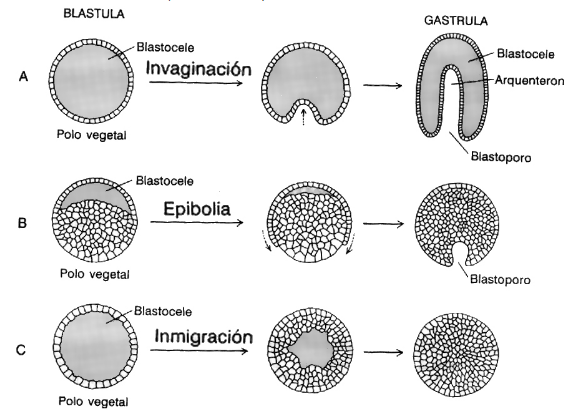
\includegraphics[width=0.7\columnwidth]{A.imagenes/ACV-ANATANIM-Gastrulacion}
    \caption[Modelos de gastrulación]{Modelos de gastrulación. A, por invaginación: las células del polo vegetal del embrión se invaginan y forman el arquénteron; la abertura al exterior es el blastoporo; B, por epibolia: las células del polo animal del embrión crecen para recubrir las del polo vegetal; en este caso el blastoporo se puede formar más tarde; C, por inmigración: las células de la pared interna de la blástula caen al interior del blastocele, formando una masa que luego se ahuecará para formar un arquénteron. Existen aún más modalidades. }
\end{figure}
\subsection{Hojas embrionarias}
Una hoja embrionaria es el conjunto de células formadoras durante el desarrollo embrionario a partir de las cuales se generarán los diversos órganos y tejidos.
\begin{itemize}[itemsep=0pt,parsep=0pt,topsep=0pt,partopsep=0pt]
    \item \textbf{Ectodermo}: 
    \begin{itemize}[itemsep=0pt,parsep=0pt,topsep=0pt,partopsep=0pt]
        \item Epidermis
        \item Sistema nervioso
        \item Boca, faringe, recto y ano.
    \end{itemize}
    \item \textbf{Endodermo}:
    \begin{itemize}[itemsep=0pt,parsep=0pt,topsep=0pt,partopsep=0pt]
        \item Tubo digestivo
        \item Glándulas anejas
        \item Células germinales
    \end{itemize}
    \item\textbf{Mesodermo}: 
    \begin{itemize}[itemsep=0pt,parsep=0pt,topsep=0pt,partopsep=0pt]
        \item Dermis
        \item Aparato circulatorio
        \item Musculatura y esqueleto (vertebrados)
        \item Aparato excretor
        \item Aparato reproductor (células no germinales)
        \item Aparato respiratorio (no faringe)
    \end{itemize}
\end{itemize}

Cada una de las estructuras se formará mediante organogénesis que es el proceso de formación del órgano a partir de las hojas embrionarias.
\subsection{Blastoporo}
El blastoporo (lugar que comunica el arquenteron con el exterior) diferencia a dos tipos de animales:
\begin{itemize}[itemsep=0pt,parsep=0pt,topsep=0pt,partopsep=0pt]
    \item \textbf{Protóstomos}: animales de segmentación espiral, del blastoporo permanece abierto y formará la boca.
    \item\textbf{Deuteróstomos}: animales de segmentación radial, el blastoporo se cierra y la boca es de neoformación.
\end{itemize}
\subsection{Formación del mesodermo}
El proceso de formación del mesodermo o embolia puede darse de dos formas:
\begin{itemize}[itemsep=0pt,parsep=0pt,topsep=0pt,partopsep=0pt]
    \item \textbf{Animales de segmentación espiral}: al ser animales con una determinación muy temprana, se puede localizar que blastómeros dan lugar al mesodermo. En este caso, es el blastómero 4D, sitá junto al blastoporo. Por un proceso de mitosis repetidas forma el mesodermo, siguiendo uno de estos tres procesos:
    \begin{itemize}[itemsep=0pt,parsep=0pt,topsep=0pt,partopsep=0pt]
        \item \textbf{Animales acelomados}: (platelmintos) todo el blastocele (cavidad interior de la blástula) se rellena de mesodermo y no forma celoma.
        \item\textbf{Animales pseudocelomados}: (nemátodos) el mesodermo se pega al ectodermo, formando una cavidad, el pseudoceloma.
        \item\textbf{Animales celomados}: (anélidos, moluscos y artrópodos) los blastómeros del mesodermo forman unas esferas huecas cuyo interior se denomina celoma. Este proceso es la esquizocelia y necesita la migración a través del blastocele hasta el ecuador.
    \end{itemize}
    \item\textbf{Animales de segmentación radial}: el mesodermo se forma por enterocelia, un proceso exclusivo de cordados y equinodermos. Al ser animales de diferenciación tardía, los blastómeros que forman el endodermoestán determinados por la posición. En la enterocelia, el mesodermo se forma a partir del endodermo: de este, y por rápidas mitosis, se forman unas invaginaciones que acaban independizándose y formando una vesículas huecas con el celoma en su interior. 
\end{itemize}
\begin{figure}[H]
    \centering
    \includegraphics[width=\columnwidth]{A.imagenes/ACV-ANATANIM-Mesodermo.jpeg}    
    \caption[Modelos de formación del mesodermo]{Modelos de formación del mesodermo. A, modelos de formación del mesodermo en animales de segmentación espiral; B, modelos de enterocelia para animales de segmentación radial.}
\end{figure}
\subsection{Desarrollo postembrionario}
Se diferencian tres tipos de ciclo:
\begin{itemize}[itemsep=0pt,parsep=0pt,topsep=0pt,partopsep=0pt]
    \item \textbf{Ciclo directo}: animales con cigotos con gran cantidad de vitelo. Esto permite a la cría desarrollarse por completo, naciendo un juvenil de apariencia similar al adulto pero de menor tamaño.
    \item\textbf{Ciclo metagenético}: se da con o sin larva. La forman dos individuos adulots que conforman dos subfases del ciclo, en una hay reproducción sexual; y en la otra, reproducción asexual. Un ejemplo son los cnidarios.
    \item\textbf{Ciclo indirecto}: la larva difiere de la morfología del adulto, llegando a no reconocerse. Propio de zigotos con poco vitelo, se diferencian varias funciones a este ciclo vital como la dispersión (en los tunicados, el adulto sésil permite que la especie colonice nuevos territorios); la alimentación juvenil (la larva se alimenta para obtener los nutrientes para poder madurar); o evitar competencia con el adulto con respecto a recursos alimentarios y que no peligre la especie. Así mismo, se diferencian dos tipos de metamorfosis:
    \begin{itemize}[itemsep=0pt,parsep=0pt,topsep=0pt,partopsep=0pt]
        \item \textbf{Gradual} o \textbf{hemimetábula}: se forman nuevas estructuras de forma gradual (por ejemplo, anfibios anuros como la rana).
        \item\textbf{Dŕastica} o \textbf{Homometábula}: para alcanzar el estado adulto, la larva pasa por un estado de crisálida donde pierde estructuras larvarias, forma otras nuevas y reacomoda y adapta estructuras para su estado final (por ejemplo, los lepidípteros).
    \end{itemize}
\end{itemize}
\subsection{Ley biogenética fundamental}
Enunciada por Haeckel, afirma que <<\textit{La ontogenia es una recapitulación abreviada de la filogenia}>>. Para que esto se cumpla, es necesario que los distintos órganos y estructuras que tengan un origen embrionarl igual o similar.
\begin{itemize}[itemsep=0pt,parsep=0pt,topsep=0pt,partopsep=0pt]
    \item \textbf{Órganos homólogos}: aquellos que aunque difieren parcialmente en morfología y/o función, tienen un mismo origen embrionario.
    \item\textbf{Órganos análogos}: aquellos que tienen una misma estructura y/o posición pero un origen embrionario diferente.
\end{itemize}
\subsection{Desarrollo embrionario de un vertebrado}
Todos los animales del subfilo \textit{vertebrados} cumplen las siguientes características:
\begin{itemize}[itemsep=0pt,parsep=0pt,topsep=0pt,partopsep=0pt]
    \item Animales triblásticos, enterocelomados, simétricos bilateralmente.
    \item Faringotremados, epineuros, con corda rodeada de vértebras y con cola postanal eviscerada.
    \item Deuteróstomos, cigotos isolecitos, de segmentación radial.
\end{itemize}

El desarrollo embrionario de un vertebrado se diferencia según la especie, variando la duración de cada fase o la cantidad de fases, pero en cierto momentos, siguiendo los principios observados de Haeckel, son parecidos. Las fases del desarrollo embrionario comunes a todos los vertebrados son:
\begin{enumerate}[itemsep=0pt,parsep=0pt,topsep=0pt,partopsep=0pt]
    \item Segmentación y gastrulación.
    \item Cierre del blastoporo.
    \item Formación de un neurodermo a partir de una sección del ectodermo , una zona de la corda (de una sección superior del endodermo) y el mesodermo (se crea por enterocelia).
    \item Formación de las cavidades celomáticas y crecimiento en forma de tubo.
    \item Cierre del neurodermo e independización de la zona de la corda.
    \item Desarrollo de:
    \begin{enumerate}[itemsep=0pt,parsep=0pt,topsep=0pt,partopsep=0pt]
        \item \textbf{Neurodermo}: crecimiento longitudinal y formación de una vesícula encefálica que dará lugar al Sistema Nervioso central. En animales con encéfalo, en su parte anterior desarrolla una vesícula encefálica que da lugar al encéfalo; mientras que su región caudal dará lugar a la médula espinal. Se encuentra hueca por dentro, formando en su interior el epéndimo.
        \item\textbf{Corda}: desarrollo longitudinal y rellenado de con células cordotonales muy grandes que acaban formando uniones ocluyentes. Sobre la corda se forman las vértebras que acaban integrandola.
        \item\textbf{Mesodermo}: se dan dos tipos de desarrollo:
        \begin{itemize}[itemsep=0pt,parsep=0pt,topsep=0pt,partopsep=0pt]
            \item \textbf{Ventral}: las dos vesículas celómicas permanecen huecos, se alargan y se unen por la región ventral. Den lugar al peritoneo.
            \item\textbf{Dorsal}: las dos secciones se dividen en tres de forma perpendicular. Las seis partes resultantes tiene, cada una tres regiones:
            \begin{itemize}[itemsep=0pt,parsep=0pt,topsep=0pt,partopsep=0pt]
                \item \textbf{Esclerodermo}: parte dorsal, da lugar al esqueleto.
                \item\textbf{Miotomo}: parte medial, da lugar a la musculatura.
                \item\textbf{Nefrotomo}: parte ventral, da lugar al aparato excretor.
            \end{itemize}
        \end{itemize}
     \end{enumerate}
\end{enumerate}
\begin{figure}[H]
    \centering
    \subfigure[Diferenciación del mesodermo.]{\includegraphics[width=0.4\columnwidth]{A.imagenes/ACV-ANATANIM-FormacionMesodermo.png}}
    \subfigure[Neurulación o fases de formación del tubo neural.]{\includegraphics[width=0.59\columnwidth]{A.imagenes/ACV-ANATANIM-DiferenciacionNeurodermo.png}}
    \caption[Diferenciación del mesodermo]{Diferenciación del mesodermo.}
\end{figure}




    \part{Metodologías de laboratorio}
     \chapter{Técnicas electroquímicas}
\section{Medición de pH}
\chapter{Técnicas de separación de sustancias}
\section{Centrifugación}
\section{Electroforesis}
\subsection{Electroforesis en gel de agarosa}
\subsection{Electroforesis en gel de poliacrilamida}
\subsection{Electroforesis 2D}
\section{Cromatografía}
\subsection{Cromatografía plana}
\subsection{Cromatografía en columna}
\chapter{Espectrometría}
\section{Espectrofotometría visible y UV}
\section{Espectrometría de masas}
\section{Resonancia magnética nuclear}
\chapter{Métodos enzimáticos}
\section{Métodos enzimáticos colorimétricos}
\section{Zimografía}
\chapter{Técnicas inmunológicas}
\section{Inmunoprecipitación}
\section{Aglutinación y fijación del complemento}
\section{Inmunofluorescencia}
\section{Inmunoanálisis}
\subsection{Radioinmunoensayo (RIA)}
\subsection{ELISA}
\section{Inmunotransferencia: Western-blot}
\section{Inmunocitoquímica}
\subsection{Inmunocitoquímica directa}
\subsection{Inmunocitoquímica indirecta}
\section{Purificación de anticuerpos}
\subsection{Producción de anticuerpos monoclonales}
\section{Técnicas de determinación de complemento}
\chapter{Técnicas de Genética y Biología molecular}
\section{Aislamiento y purificación de ácidos nucleicos}
\subsection{Método de fenol-cloroformo-isoamílico}
\subsection{Método de isotiocianato de guanidina-fenol-cloroformo}
\section{Síntesis de ADNc: retrotranscripción}
\section{PCR}
\subsection{RT-PCR}
\subsection{PCR anidada}
\subsection{PCR múltiple}
\subsection{PCR \textit{in situ}}
\subsection{PCR cuantitativa en tiempo real}
\section{Clonación}
\section{Secuenciación}
\subsection{Método químico de Maxwell-Gilbert}
\subsection{Método enzimático de Sanger}
\subsection{Secuenciación automática}
\section{Southern-blot}
\section{Microarrays}
\section{RFLPs}
\section{MLPA}
    \part{Epidemiología}
    % SEC I - Introducción
     \chapter{Introducción}
\section{Introducción: Epidemiología y salud}
La Epidemiología es la disciplina científica que estudia la frecuencia y distribución de la enfermedad en la población y sus determinantes.
\begin{table}[H]
	\centering
	\begin{tabular}{M{2.5cm}N{13.5cm}}
		\rowcolor{black}\textcolor{white}{\textbf{Término}}&\textcolor{white}{\textbf{Definición}}\\
		Estudio&Incluye: vigilancia, observación. test de hipótesis, investigación analítica y experimentación.\\
		\rowcolor{hiperlightgray}Distribución&Referencia a análisis de: tiempos, personas, sitios y clases sociales.\\
		Determinantes&Factores que influyen en la salud: biológicos, químicos, físicos, sociales, culturales, económicos, genéticos y comportamentales\\
		\rowcolor{hiperlightgray}Estados y eventos relacionados con la salud&Referencia a: enfermedades, causa de la muerte, comportamiento (tabaquismo, $\dots$), estado de salud positivos, usod de servicios sanitarios,$\dots$\\
		Poblaciones específicas& Incluye a aquellas con características diferenciales como la ocupación de los grupos.\\
		\rowcolor{hiperlightgray}Aplicación de prevención y control&Objetivos de salud pública para promover, proteger o restaurar la salud.\\
		\hline
	\end{tabular}
	\caption{Terminología útil en epidemiología.}
\end{table}

Frente a la medicina clínica, que estudia individualmente al paciente, la epidemiología estudia a la población en su conjunto. La epidemiología parte de la premisa de que la enfermedad y los problemas de salud no se distribuyen aleatoriamente en una población, sino que existen, en cada individuo, unos características que predisponen a la enfermedad o protegen de ella, pudiendo ser factores genéticos y/o exposición a ciertos riesgos sociales y ambientales. La epidemiología permite:
\begin{itemize}[itemsep=0pt,parsep=0pt,topsep=0pt,partopsep=0pt]
	\item Estudio histórico de la enfermedad: monitorización o vigilancia de tendencias temporales de la enfermedad.
	\item Identificación de síndromes.
	\item Diagnóstico de salud de la comunidad.
	\item Investigación etiológica: identificación de factores que llevan de la salud a la enfermedad.
	\item Evaluación de servicios y de intervenciones sanitarias como el tratamiento médico y campañas de salud pública. Llevan de la enfermedad a la salud.
\end{itemize}

Dentro de la epidemiología se pueden distinguir:
\begin{itemize}[itemsep=0pt,parsep=0pt,topsep=0pt,partopsep=0pt]
	\item \textbf{Epidemiología descriptiva}: estudia la frecuencia y distribución de las enfermedades y problemas de salud, observando los hechos básicos de la distribución en términos de persona, lugar y tiempo. Se basa en estudios descriptivos, individuales (descripción de un caso o series de casos) o poblaciones de región geográfica o administrativa (estudios ecológicos y encuestas).
	\item \textbf{Epidemiología analítica}: estudia los determinantes de la enfermedad, pone a prueba una hipótesis acerca de una relación entre causa y enfermedad, relacionando la exposición de interés con la enfermedad de interés. Se articula en torno a estudios analíticos de tipo observacional (estudios transversales (encuestas), estudios de cohortes y de casos-controles) y experimentales (ensayos clínicos o ensayos de intervención).
\end{itemize}

El término salud se puede definir como: Estado de completo bienestar físico, mental y social y no sólo como ausencia de enfermedad (OMS, 1948); recurso de la vida diaria, concepto que aúna recursos sociales y personales además de aptitudes físicas (Carta de Ottawa, 1986); o como ausencia de enfermedad.
\section{Diagnóstico, pronóstico y tratamiento}
La epidemiología resulta también fundamental no sólo para la salud pública sino también en la práctica clínica. La práctica de la medicina depende de datos poblacionales. El médico aplica un modelo de probabilidad basado en poblaciones al paciente a tratar. Los conceptos y datos basados en la población subyacen a los procesos fundamentales de la práctica clínica: <<diagnóstico + pronostico + tratamiento>>.

Los datos disponibles de enfermedad pueden ser útiles para indicar un diagnóstico, aunque no sea concluyente. El médico aplica un modelo de probabilidad al paciente basado en poblaciones. Los pronósticos de tiempo de vida o enfermedad se basan en la experiencia del médico con un número muy amplio de pacientes que han tenido la misma enfermedad, a los que se observó en el mismo estadio de la enfermedad y que recibieron el mismo tratamiento, es decir, se basa en datos poblacionales.

La selección del tratamiento adecuado se basa en la población. Los ensayos clínicos con distribución aleatoria que investigan los efectos de un tratamiento en un grupo grande de pacientes son el medio ideal para identificar el tratamiento más eficaz y clinicamente  adecuado. Aunque parezca que prevención y tratamiento son actividades excluyentes, la prevención es una parte integral de salud pública y práctica clínica. La epidemiología sirva para planificar y poner en marcha programas de prevención, o para dirigir investigaciones clínicas que ayudan a controlar la enfermedad.

Ejemplos de usos de la epidemiología en la práctica clínica son el descubrimiento de la vacuna frente a la viruela por Edward Jenner, al descubrir que las vaqueras en contacto con vacas infectadas de la viruela bovina no contraian la enfermedad; o el descubrimiento del modo de transmisión de \textit{Vibrio Cholerae} por John Snow, patógeno de la cólera, a través de aguas infectadas, al apreciar que disminuyen los casos en Londres por el cambio de lugar de extracción de aguas (es un caso de expermiento natural, el investigador no modifica la variable, lo hace el ambiente).
\section{Sistema de información sanitaria}
Los sistemas de información sanitaria son un conjunto ordenado de datos organizados con objeto de suministrar información adecuada para informar del estado de salud, de las necesidades sanitarias y dar apoyo a las intervenciones en salud pública. Sirven para valorar la situación sanitaria poblacional, tener sistemas de vigilancia de salud, establecimiento de programas de salud e investigación.

\begin{table}[H]
	\centering
	\begin{tabular}{M{2.5cm}N{4cm}N{5.25cm}N{4cm}}
		\rowcolor{black}\textcolor{white}{\textbf{}}&\textcolor{white}{\textbf{Registros}}&\textcolor{white}{\textbf{Encuestas}}&\textcolor{white}{\textbf{Sist. Notificaciones}}\\
		Base poblacional&
			\begin{tabular}{N{4cm}}
				Natalidad\\
				Mortalidad\\
				Muertes fetales\\
				Enfermedades\\
			\end{tabular}&
			\begin{tabular}{N{5.25cm}}
				Encuesta de salud\\
				Encuesta Nacional de Salud\\
				Encuesta de Población Activa\\
			\end{tabular}&
			\begin{tabular}{c}
				CMBD\\
			\end{tabular}\\
		\rowcolor{hiperlightgray}Procedentes de servicios sanitarios&CMBD&&EDO\\
		\hline
	\end{tabular}
	\caption[Registros de información sanitaria]{Registros de información sanitaria: tipos de registros y la información que dan. Siglas: \textit{CMBD}: Conjunto Mínimo Básico de Datos; \textit{EDO}: Enfermedad de Declaración Obligatoria.}
\end{table}

Los registros de enfermedades son entidades encargadas de recoger, almacenar, analizar e interpretar los datos sobre personas con una determinada enfermedad. El objetivo de estos registros en una población es conocer el número de casos diagnosticados en un periodo definido de tiempo y residentes en el área geográfica abarcada. Los datos de utilidad para el control de enfermedades se usan en etiología, prevención primaria y secundaria, planificación sanitaria y atención al paciente.

La información de los registros procede de todos los centros sanitarios existentes en la población. La detección de los casos se realiza a través de la información recibida con periodicidad en el registro procedente de servicios de documentación o laboratorios de anatomía patológica. Es de gran utilidad esta información, así como la facilitada por otros servicios hospitalarios en los que se diagnostica o trata estas enfermedades.
    % SEC II - Tipos de estudio
     \chapter{Tipos de estudio y diseño epidemiológico}
\section{Introducción}
El escoger el diseño de expermiento adecuado es un paso fundamental en la investigación epidemiológica, dado que cada tipo de diseño tiene sus puntos fuertes y debilidades. Los epidemiólogos han de considerar todas las fuentes de sesgo y confusión y tratar de reducirlas. Las temáticas éticas son también importantes.Los estudios epidemiológicos pueden clasificarse en:
\begin{itemize}[itemsep=0pt,parsep=0pt,topsep=0pt,partopsep=0pt]
	\item \textbf{Observacionales}: en ellos, el investigador mide pero no interviene. Pueden ser:
	\begin{itemize}[itemsep=0pt,parsep=0pt,topsep=0pt,partopsep=0pt]
		\item \textbf{Descriptivos}: La investigación se limita a describir la frecuencia de una enfermedad en una población (con frecuencia es el primer paso de la investigación).
		\item \textbf{Analíticas}: analizan la relación entre estado de salud y otras variables.
	\end{itemize}
	Normlamnete, la mayoría de estudios epidemiológicos tiene un componente de ambos. Así mismo, son frecuentes los estudios puramente descriptivos, y muy raros los analíticos.
	\item \textbf{Experimentales}: los estudios experimentales suponen un intento activo de cambio de los determinantes de una enfermedad como la exposición o un comportamiento - o el progreso de la enfermedad con un tratamiento, de manera igual a la experimentación en otras ciencias. Sin embargo, ellos son sujetos a obligaciones extra, desde que la salud de las personas puede estar en cuestión. En su mayoría incluye:
	\begin{itemize}[itemsep=0pt,parsep=0pt,topsep=0pt,partopsep=0pt]
		\item Aleatorización controlada de pruebas usando pacientes como sujetos.
		\item Estudio de campo con participantes sanos.
		\item Estudios comunitarios con los propios participantes de la comunidad.
	\end{itemize}
\end{itemize}
\section{Tipos de estudios}
\subsection{Estudios descriptivos}
Una simple descripción del estado de salud de una comunidad, basada en datos gratuitos rutinarios u obtenidos en encuestas, siendo normalmente el primer paso en la investigación epidemiológica. En muchos países es suministrado por centros estadísticos nacionales. Los estudios puros estadísticos no analizan causas y efectos. Normalmente, los estudios descriptivos son o están basados en estadísticas de mortalidad, examinando variables de muerte por edad, sexo, etnia,$\dots$ durante periodos específicos de tiempo en varios países.
\subsection{Estudios ecológicos}
Resultan útiles para generar hipótesis. En un estudio ecológico, las unidades de análisis son grupos de personas antes que individuos. Cada una de las observaciones necesitaría ser testada mediante control para excluir la posibilidad de que otras características, como enfermedades graves en diferentes poblaciones, no cuentan para la relación.

Los estudios ecológicos también pueden ser hechos mediante comparación de poblaciones en diferentes sitios al mismo tiempo o en series de tiempo por comparación de la misma población en un sitio en tiempos diferentes.
\subsubsection{Falacia ecológica}
Un sesgo o falacia ecológica resulta si conclusiones inapropiadas son deducidas en base a datos ecológicos. Cada inferencia ecológica, aunque limitada puede proveer un comienzo fructífero para un trabajo epidemiológico más detallado.
\subsection{Estudios transversales}
Miden la prevalencia de una enfermedad. En un estudio transversal, la medida de exposición y efecto se hacen al mismo tiempo. No es sencillo calcular las razones que muestran las asociaciones en estudios transversales. La cuestión clave es descubrir si la exposición precede o sigue al efecto. Si los datos de exposición se muestra que la exposición es anterior a cualquier efecto, los datos de un estudio transversal pueden ser tratados como datos generados por un estudio de cohortes.

Los estudios transversales son relativamente fáciles y baratos de gestionar y son útiles para investigar exposiciones que son características inalterables de individuos como etnia, grupo sanguineo, $\dots$ En brotes repentinos de enfermedades, un estudio transversal para medir varias exposiciones puede ser el primer paso más conveniente en la investigación de la causa.

Los datos de estudios transversales son útiles en la evaluación de las necesidades de cuidados de salud de las poblaciones. Los datos de repetidas encuestas transversales utilizando muestras aleatorias independientes con definiciones estandarizadas y métodos de entrevista provee de útiles indicaciones de tendencias. Cada encuesta tendría un propósito claro. Las encuestas válidas necesitan de cuestionarios bien diseñados, una muestra apropiada de suficiente tamaño y un buen ratio de respuestas.

Gran cantidad de países conducen encuestas transversales de muestras representativas de su población, centrandose en características demográficas e individuales, enfermedades y hábitos de vida saludable. Frecuencia de enfermedades y factores de riesgo pueden ser examinados en relación a edad, sexo y etnia.
\subsection{Estudios de Casos-Controles}
Los estudios de casos-controles proveen una relativamente simple vía para investigar la causa de las enfermedades raras. Se incluyen personas con una enfermedad (u otra variable de resultados) de interés y un control adecuado (comparación de referencia), un grupo de personas no afectadas por la enfermedad u otra variable de resultados. El estudio compara la incidencia de las posibles causas en casos y controles. El investigador recoge datos de la incidencia de la enfermedad en un punto en el tiempo y de la exposición en un punto de tiempo anterior.

Los estudios casos-controles son longitudinales. Han sido llamados retrospectivos dado que el investigador mira atrás desde la enfermedad a las posibles causas. Esto puede ser confuso porque los términos retrospectivo y futurible son también usados para describir el momento de recolección de datos en relación a la fecha actual. En este sentido, los estudios caso-control pueden ser retrospectivos, cuando todos los datos tratan sobre el pasado, o futuribles cuando la recolección de información continúa con el paso del tiempo.
\begin{figure}[H]
	\centering
	\includegraphics[width=0.5\columnwidth]{A.imagenes/ACV-EPI-CasosControles}
	\caption{Ejemplo de intervención en estudio de casos-controles.}
\end{figure}
\subsubsection{Selección de casos y controles}
Un estudio de casos-controles comienza con la selección de casos. Estos representarían todos los casos en un grupo poblacional espcífico. Los casos son seleccionados en base a la enfermedad y no a la exposición. Los controles son personas sin la enfermedad. Un aspecto fundamental y exigente de los estudios basados en casos-controles es encontrar una manera de coste apropiado para identificar y enrolar sujetos controles para mostrar la prevalencia de la exposición en la población que genera los casos. Además, la elección de controles y casos debe no estar influenciada por el estado de exposición, que debe ser determinado de la misma manera en ambos. No es necesario ser inclusivo, de hecho puede restringirse a cualquier subgrupo específico.

Los controles representan presonas quienes habrían estado designados al estudio como casos si hubieran contraído la enfermedad. Idealmente, los estudios de caso-control utiliza nuevos casos (incidentes) para evitar la dificultad de separar factores que intervienen en la causalidad y supervivencia (o recuperación), aunque los estudios han sido, con frecuencia, conducidos usando datos de prevalencia (por ejemplo, estudios de caso-control de malformaciones genéticas). Los estudios de casos-controles estiman el riesgo relativo de enfermedad, pero no determinan de forma absoluta la incidencia de enfermedad.
\subsubsection{Exposición}
Un aspecto importante de los estudios de caso-control es la determinación de comienzo y duración de la exposición para casos y controles. En el diseño de casos-controles, el estado de exposición de los casos es normalmente determinado después del desarrollo de la enfermedad (datos retrospectivos) y normalmente por cuestionarios directos de afectados o familiares y amigos. Las respuestas de los informantes puede estar influenciada por el conocimiento de la hipótesis bajo investigación o la experiencia propia de la enfermedad.

La exposición se determina a veces por parámetros bioquímicos (por ejemplo, plomo en sangre o cadmio en orina), los cuales pueden no representar la relevancia de exposiciones pasadas. Por ejemplo, el plomo en sangre a los 6 años no es un buen indicador de la exposición a los 1 ó 2 años, edades con gran sensibilidad al plomo. Este problema puede ser evitado si la exposición puede ser estimada por un sistema establecido de registro (guardado de resultado de test de sangre rutinario) o si los estudios caso-control son llevados a cabo de forma prospectiva, de manera que los datos son recogidos antes del desarrollo de la enfermedad.
\subsubsection{\textit{Odds ratio} o proporción de razones}
La asociación de exposición y enfermedad (riesgo relativo) en un estudio de caso-control se mide mediante el cálculo de <<\textit{odds ratio}>> (OR) que es la proporción de las razones de exposición entra la razones de los controles. Las \textit{odds ratio} es similar a la proporción de riesgo, especialmente si la enfermedad es rara. Para la proporción de razones sea una buena aproximación, los casos y los controles deben ser representativos de la población general con respecto a la exposición. Sin embargo, debido a que la incidencia de la enfermedad es desconocida, el riesgo absoluto no puede ser calculado. Una proporción de razones ha de ser acompañado de un intervalo de confianza sobre el punto estimado.
\begin{table}[H]
	\centering
	\begin{tabular}{
			>{\columncolor[HTML]{000000}}l 
			>{\columncolor[HTML]{000000}}l lll}
		{\color[HTML]{FFFFFF} } & {\color[HTML]{FFFFFF} } & \multicolumn{2}{l}{\cellcolor[HTML]{000000}{\color[HTML]{FFFFFF} Exposición}} &  \\
		{\color[HTML]{FFFFFF} } & {\color[HTML]{FFFFFF} } & \cellcolor[HTML]{000000}{\color[HTML]{FFFFFF} Sí} & \cellcolor[HTML]{000000}{\color[HTML]{FFFFFF} No} &  \\
		\cellcolor[HTML]{000000}{\color[HTML]{FFFFFF} } & {\color[HTML]{FFFFFF} Sí} & A & B &  \\
		\multirow{-2}{*}{\cellcolor[HTML]{000000}{\color[HTML]{FFFFFF} Enfermedad}} & {\color[HTML]{FFFFFF} No} & \cellcolor[HTML]{DAE8FC}C & \cellcolor[HTML]{DAE8FC}D &
	\end{tabular}
	\caption[Cuadro de Punnet u \textit{Odds ratio}]{Cuadro de Punnet u \textit{Odds ratio}: en esta tabla se clasifican los distintos casos por su grado de exposición.}
\end{table}
\begin{center}
	\begin{equation}
		OR = \dfrac{A\cdot D}{B\cdot C}
	\end{equation}
	\captionof{Ecuacion}[Ecuación de \textit{Odds Ratio}]{Ecuación de \textit{Odds ratio}, leida como la posiblidad de un sujeto expuesto a desarrollar la enfermedad.}
\end{center}
\subsection{Estudios de cohortes}
Los estudios de cohortes comienzan con un grupo de presonas libres de la enfermedad y que son clasificados en subgrupos de acuerdo a la exposición a una causa potencial de enfermedad o resultado. Las variables de interés son especificados y medidos y la cohorte entera es seguida para observar como el ulterior desarrollo de nuevos casos de enfermedad (u otro resultado) difiere entre grupos con y sin exposición. Dado que los datos de exposición y enfermedad se refieren a diferentes puntos en el tiempo, los estudios de cohortes son longitudinales. Los estudios de cohortes son estudios de futuro, término confuso que puede ser evitado, ya que se refiere al momento de recabación de datos, no a la relación exposición-efectos, pudiendo haber estudios retrospectivos o de futuro.

Los estudios de cohorte proveen la mejor información sobre la causa de la enfermedad y la medida más directa del riesgo de contraer la enfermedad. Aunque conceptualmente simples, son muy complejos y pueden requerir largos periodos de tiempo de seguimiento desde que la enfermedad puede ocurrir un tiempo largo de exposición. Muchas exposiciones son investigadas durante largos periodos en la naturaleza y la precisa información sobre ellas requiere largos periodos de recogida de datos.

En situaciones con repetidas y puntuales exposiciones, la relación causa-efecto para efectos puntuales puede ser obvio, pero los estudios de cohortes son también usados para investigar efectos tardíos o crónicos. Como un estudio de cohortes empieza con gente expuesta y no expuesta, la dificultad de medida o el hallar datos existentes en exposiciones en gran medida determina la viabilidad de realización de estos. Si la enfermedad es rara en grupos expuestos y no expuestos puede provocar también problemas en la obtención en grupos suficientemente grandes de estudio.

El coste de un estudio de cohortes puede ser reducido usando fuentes rutinarias de información sobre mortalidad y morbilidad, como registros de enfermedades o registros nacionales de muertes como parte del seguimiento. Un tipo especial de estudios de cohortes con los estudios de gemelos, donde el factor de variación genética (entre gente expuesta y no expuesta a un factor particular) puede ser eliminado. Como estudios ha provisto de fuertes evidencias para una variedad de relaciones causa-efecto para enfermedades crónicas.
\begin{figure}[H]
	\centering
	\includegraphics[width=0.5\columnwidth]{A.imagenes/ACV-EPI-Cohortes}
	\caption{Ejemplo de intervención en estudio de cohortes.}
\end{figure}
\subsubsection{Estudios de cohortes históricos}
Los costes pueden ser reducidos usando cohortes históricas (identificadas en base a crónicas de exposición previas). Se llaman así porque toda exposición y efecto (enfermedad) ha sido recogida antes del comienzo del estudio actual. Este orden de diseño es muy común para estudios que relacionan cáncer y exposiciones laborales.
\subsubsection{Estudios caso-control integrados}
El diseño de estudios caso-control integrados hace menos caros a los estudios de cohortes. Los casos y los controles son ambos escogidos de una cohorte definida para el cual alguna información sobre exposición y factores de riesgo está ya disponible. Información adicional de nuevos casos y controles, particularmente seleccionados para el estudio son recogidos y analizados. Estos diseños son particularmente útiles cuando la medida de la exposición es cara.
\section{Epidemiología experimental}
La intervención o experimentación implica intenta cambiar una variable en uno o más grupos de personas. Esto puede significar la eliminación de un factor dietético que se piense que provoca alergia, o la prueba de un nuevo tratamiento sobre un nuevo tratamiento sobre un grupo seleccionado de pacientes. Los efectos de una intervención han de ser medidos mediante comparación de resultados con el grupo control. Puesto que las intervenciones están estrictamente reguladas por los estudios de protocolo, las consideraciones éticas son de importancia capital en el diseño de estudios. Por ejemplo, ningún paciente debe serle denegado el tratamiento apropiado como resultado de la participación en un experimento, y este debe ser testado a la luz del conocimiento actual. El consentimiento informado es requerido en todos los casos.
\subsection{Estudios clínicos}
Un estudio clínico es un experimento epidemiológico diseñado para estudiar los efectos de una intervención particular, normalmente un tratamiento para una enfermedad específica. Los sujetos en el estudio poblacional son aleatoriamente asignados a grupos control o de intervención, y los resultados son calculados por comparación. Para asegurar que los grupos que están siendo comparados son equivalentes, los pacientes son asignados aleatoriamente. Si la selección inicial y la aleatorización se hicieron adecuadamente, los grupos control y de tratamiento serán comparables al inicio de la investigación; cualquier diferencia entre grupos son acontecimientos no afectados por sesgos conscientes o inconscientes de los investigadores.
\begin{figure}[H]
	\centering
	\includegraphics[width=0.5\columnwidth]{A.imagenes/ACV-EPI-EstudioClinico}
	\caption{Ejemplo de intervención en estudio clínico.}
\end{figure}
\subsection{Estudios de campo}
Los estudios de campo implica a la población sana pero presupuesta a estar en riesgo. La recolección de datos se toma <<en el campo>>, normalmente entre personas no institucionalizadasde la población general. Entonces los sujetos están libres de enfermedades y el propósito es prevenir las enfermedades que pueden ocurrir con relativamente baja frecuencia. Suelen ser logisticamente complejos y suponen un esfuerzo costoso (un ejemplo fue la vacuna frente a la polio de Salk, con un millón de infantes vacuandos).

Los estudios de campo pueden ser usados para evaluar intervenciones apuntando a reducir la exposición sin necesariamente medir los sucesos de los efectos de salud. Cada estudio de intervención puede hacerse en menor escala y con menor coste así como no implicar un largo seguimiento o medida de los resultados de enfermedades.
\subsection{Pruebas comunitarias}
En este tipo de experimentos, el grupo de tratamiento son comunidades antes que individuos. Esto es particularmente apropiado para enfermedades que son influenciadas por las condiciones sociales y para esfuerzos de prevención sobre grupos de comportamiento.
\subsubsection{Limitaciones}
Una limitación de estos estudios es que sólo un pequeño número de comunidades puede ser incluido y la distribución aleatoria de las comunidades no es normalmente viable. Otros métodos son requeridos para asegurar que cualquier diferencia encontrada al finalizar el estudio pueden ser atribuidas a la intervención preferiblemente que a diferencias inherentes entre comunidades. Además es difícil aislar comunidades donde la intervención tiene lugar frente a cambios sociales generales que pueden estar ocurriendo. Las limitaciones del diseño, especialmente frente a inesperadamente largos, los factores de riesgo favorables cambian en sitios control, siendo dificil calcularlos. Como consecuencia, las conclusiones definitivas sobre la efectividad global de los intentos internacionales no son siempre positivos.
\begin{table}[H]
	\centering
	\begin{tabular}{M{2.15cm}N{2.15cm}N{1.8cm}N{2cm}N{2.5cm}N{1.8cm}N{2cm}}
		\rowcolor{black}\textcolor{white}{\textbf{Estudios}}&\textcolor{white}{\textbf{Descriptivo}}&\textcolor{white}{\textbf{Analíticos}}&\textcolor{white}{\textbf{Ecológicos}}&\textcolor{white}{\textbf{Transversales}}&\textcolor{white}{\textbf{Caso-Control}}&\textcolor{white}{\textbf{Cohortes}}\\
		Unidad de estudio&---&---&Población&Individuos&Individuos&Individuos\\
		Enfermedades raras&-&-&+&-&+&-\\
		\rowcolor{hiperlightgray}Causas raras&-&-&+&-&-&+\\
		Múltiples efectos de causa&-&-&+&+&-&+\\
		\rowcolor{hiperlightgray}Multiples exposiciones y determinantes&-&-&+&+&+&+\\
		Medidas relacionadas con tiempo&-&-&+&-&+&+\\
		\rowcolor{hiperlightgray}Medida directa incidencia&-&-&-&-&+&+\\
		Investigaciones largo tiempo&-&-&-&-&+&-\\
		\hline
	\end{tabular}
	\caption{Aplicaciones de los estudios epidemiológicos.}
\end{table}
\section{Errores potenciales en estudios epidemiológicos}
La investigación  aspira a proveer de medidas exactas de la incidencia de enfermedades u otro resultado en salud. Sin embargo, hay muchas posibilidades de errror en la medida que debe ser minimizado y calculado aquél que no puede ser eliminado. Los tipos de error:
\begin{itemize}[itemsep=0pt,parsep=0pt,topsep=0pt,partopsep=0pt]
	\item \textbf{Error aleatorio}: ocasionados por variaciones en la medida de la muestra, debido únicamente al azar, determinando un valor que diverge del real, causando inexactitud en la medida. El error aleatorio nunca puede ser eliminado desde que se estudia una muestra de la población. Son tres los tipos, no pudiéndose eliminar por un estudio sobre una muestra:
	\begin{itemize}[itemsep=0pt,parsep=0pt,topsep=0pt,partopsep=0pt]
		\item \textbf{Variación biológica individual}: Siempre ocurre y la medida no es perfecta.
		\item\textbf{Error de muestreo}: causado por el hecho de que una pequeña muestra no es representativa de todas las variables poblacionales. La mejor forma de reducirla es aumentar el tamaño del estudio.
		\item\textbf{Error de medida}: el error de medida puede ser reducido por severos protocolos, y haciendo medidas individuales tan precisas como sean posibles. Es preciso conocer el método de medida usado y los errores que pueden producir. Los laboratorios han de contar con procedimientos de control de calidad (exactitud y precisión de medidas).
	\end{itemize}
	\item\textbf{Tamaño de muestra}: La muestra debe ser lo suficientemente grande para tener el suficiente poder estadístico para detectar las diferencias importantes estimadas. El tamaño al final se determina por consideraciones logísticas y financieras, y ha de de hacerse un compromiso entre los costes y el tamaño de la muestra. La siguiente información es necesaria antes de que los cálculos se hagan:
	\begin{itemize}[itemsep=0pt,parsep=0pt,topsep=0pt,partopsep=0pt]
		\item Requiere un nivel de significación estadística con la capacidad de detectar la diferencia.
		\item Nivel de error aceptable o se arriesga a perder el efecto real.
		\item Magnitud del efecto bajo investigación.
		\item Tamaño relativo de los grupos a comparar.
	\end{itemize}
	\item\textbf{Precisión}: la precisión del estudio puede ser también mejorada asegurandose de que los grupos son del tamaño relativo apropiado. Este es frecuentemente un asunto que afecta a estudios de caso-control cuando se requiere una decisión sobre el número de controles para cada caso. Si no es posible, ser definitivo sobre el ratio ideal de controles sobre casos, entonces depende de los costes relativos de recopilar casos y controles. En general, sin embargo, podría haber un pequeño punto donde se puede tener más cuatro controles por caso. Es importante asegurar que hay la suficiente similitud entre casos y controles cuando los datos son analizados por edad, grupo, o clase social, $\dots$ Si hay más casos, y solo unos pocos controles, el estudio podría no tener en cuenta la confusión por ciertos factores.
	\item\textbf{Error sistemático}: el error o sesgo sistemático acontece cuando los resultados difieren de una manera sistemática de los valores reales. Un estudio con un pequeño error sistemático es altamente exacto. La exactitud no se ve afectada por el tamaño de la muestra. Las posibles fuentes de error sistemático son muchos y variados, siendo los principales:
	\begin{itemize}[itemsep=0pt,parsep=0pt,topsep=0pt,partopsep=0pt]
		\item \textbf{Sesgo o error de selección}: ocurre cuando hay una diferencia sistemática entre las características de la gente seleccionada para un estudio y las características de quienes no están. Un origen obvio del sesgo ocurre cuando los participantes se seleccionan así mismos para un estudio, o porque ellos están enfermos o porque están preocupados por una exposición. Si los individuos entran o permanecen en un estudio que tiene diferentes características de aquellos quienes no fueron seleccionados inicialmente, o quien salió antes de terminar, el resultado es una estimación parcial de la asociación entre exposición y resultado. Un importante sesgo de selección se introduce cuando la enfermedad o el factor bajo investigación hace a la gente no útil para el estudio (trabajadores que abandonan el trabajo por molestias provocadas por la exposición). En cada estudio epidemiológico necesita un diseño que cuente con el sesgo.
		\item \textbf{Sesgo de medida o clasificación}:
	\end{itemize}
\end{itemize}
    % SEC III - Medidas Frecuencia
     \chapter{Medidas de frecuencia}
La epidemiología analítica se sirve de:
\begin{itemize}[itemsep=0pt,parsep=0pt,topsep=0pt,partopsep=0pt]
	\item \textbf{Frecuencias absolutas}: simplemente, el número de individuos por categorías. No permite comparar.
	\item\textbf{Frecuencias relativas}: número de individuos de la categoría con respecto a la población total.
	\begin{center}
		\begin{equation}
		F_R = \dfrac{\mbox{N individuos}}{\mbox{Total}}
		\end{equation}
		\captionof{Ecuacion}[Frecuencia relativa]{Frecuencia relativa: se lee <<El X de cada 10/100 sufre Y>>.}
	\end{center}
	\item\textbf{Proporción}: cociente de dos frecuencias absolutas donce el númerador está contenido en el denominador.
	\begin{center}
		\begin{equation}
		P = \dfrac{A}{A + B}
		\end{equation}
		\captionof{Ecuacion}[Proporción]{Proporción: se lee <<El X\% de los expuestos posee la característica Y>>.}
	\end{center}
	\item\textbf{Razón}: Cociente en el que el numerador no está contenido en el denominador. Compara fenómenos.
	\begin{center}
		\begin{equation}
		R = \dfrac{A}{B}
		\end{equation}
		\captionof{Ecuacion}[Razón]{Razón: se lee <<Por cada X individuos de B, hay Y de A>>.}
	\end{center}
	\item\textbf{Odds}: Probabilidad de que se produzca un evento entre la que no ocurra.
	\begin{center}
		\begin{equation}
		\mbox{Odds} = \dfrac{P_{(A)}}{1 - P_{(A)}}
		\end{equation}
		\captionof{Ecuacion}[Odds]{Odds: se lee <<Por cada X que no sufren la enfermedad, hay 1 que sí>>.}
	\end{center}
	\item\textbf{Tasa}: Razón de cambio entre dos magnituds en la que el denominador incluye el tiempo.
	\begin{center}
		\begin{equation}
		\mbox{Tasa} = \dfrac{A}{B\left(\frac{\mbox{udd}}{\mbox{tiempo}}\right)}
		\end{equation}
		\captionof{Ecuacion}[Tasa]{Tasa: se lee <<El X \% de los expuestos han desarrollado Y en Z tiempo>>.}
	\end{center}
	\item\textbf{Prevalencia}: proporción de individuos de una población que padecen una enfermedad. Se usa en estudios transversales y de casos-controles. Se puede indicar a modo de periodo, se toma la población en un determinado espacio de tiempo.
	\begin{center}
		\begin{equation}
		\mbox{Prevalencia} = \dfrac{\mbox{N casos}}{\mbox{Total}}
		\end{equation}
		\captionof{Ecuacion}[Prevalencia]{Prevalencia: se lee <<Hay X casos de cada $10^N$ de individuos enfermos>>.}
	\end{center}
	\item\textbf{Incidencia}: medido en personas afectadas/año, es el número de casos nuevos que se desarrollan en una población durante un periodo de tiempo. No indica un sequimiento uniforme, la población se restringe a los que pueden padecer la enfermedad y puede indicar recurrencias. Se diferencia:
	\begin{itemize}[itemsep=0pt,parsep=0pt,topsep=0pt,partopsep=0pt]
		\item \textbf{Incidencia acumulada}: probabilidad de enfermedad total en la población de riesgo. Se diferencia entre una incidencia acumulada epidémica (durante epidemias, permite el seguimiento durante el periodo epidémico), de la tasa de letalidad (fallecidos por la enfermedad).
		\begin{center}
			\begin{equation}
			I_A = \dfrac{\mbox{Casos nuevos}}{\mbox{Población inicio}}
			\end{equation}
			\captionof{Ecuacion}[Prevalencia]{Prevalencia: se lee <<Hay X casos de cada $10^N$ de individuos enfermos>>.}
		\end{center}
		\item\textbf{Tasa de incidencia}: cociente entre casos nuevos de una enfermedad ocurridos durante el periodo y la suma de todos los tiempos de observación. Necesita de un riesgo constante. Suele ser un denominador adecuado de la enfermedad.
		\begin{center}
			\begin{equation}
			T_I = \dfrac{\mbox{Casos nuevos}}{\sum\mbox{Tiempos individuales}}
			\end{equation}
			\captionof{Ecuacion}[Prevalencia]{Prevalencia: se lee <<Hay X casos de cada $10^N$ de individuos enfermos>>.}
		\end{center}
	\end{itemize}
	\item\textbf{Otros}:
	\begin{itemize}[itemsep=0pt,parsep=0pt,topsep=0pt,partopsep=0pt]
		\item \textbf{Tasa de nacimiento}:
		\begin{center}
			\begin{equation}
				T_{Nacimiento} = \dfrac{\mbox{Nacimientos vivos}}{\sum\mbox{Población en edad media}}
			\end{equation}
			\captionof{Ecuacion}{Tasa de nacimiento.}
		\end{center}
		\item\textbf{Tasa de fertilidad}:
		\begin{center}
			\begin{equation}
				T_{Fertilidad} = \dfrac{\mbox{Nacimientos vivos}}{\sum\mbox{Mujeres entre 15 y 45}}
			\end{equation}
			\captionof{Ecuacion}{Tasa de fertilidad.}
		\end{center}
		\item\textbf{Tasa de mortalidad infantil}:
		\begin{center}
			\begin{equation}
				T_{Mort Infant} = \dfrac{\mbox{Infantes muertos}}{\sum\mbox{Nacimientos vivos}}
			\end{equation}
			\captionof{Ecuacion}{Tasa de mortalidad infantil.}
		\end{center}
		\item\textbf{Tasa de mortinatos}:
		\begin{center}
			\begin{equation}
				T_{Mortinato} = \dfrac{\mbox{Muertes intrauterinas (28 semanas)}}{\sum\mbox{Total nacimientos}}
			\end{equation}
			\captionof{Ecuacion}{Tasa de mortinatos.}
		\end{center}
		\item\textbf{Tasa de mortalidad perinatal}:
		\begin{center}
			\begin{equation}
				T_{Mort Perinat} = \dfrac{\mbox{Mortinatos + muerte en 1 semana}}{\sum\mbox{Total nacimientos}}
			\end{equation}
			\captionof{Ecuacion}{Tasa de mortalidad perinatal.}
		\end{center}
	\end{itemize}
\end{itemize}
\begin{table}[H]
	\centering
	\begin{tabular}{M{2.5cm}N{3.5cm}N{3.5cm}N{3.5cm}}
		\rowcolor{black}\textcolor{white}{\textbf{Tipo medida}}&\textcolor{white}{\textbf{Proporción}}&\textcolor{white}{\textbf{}}&\textcolor{white}{\textbf{Tasa}}\\
		Equivalencia&Prevalencia&Riesgo&Tasa de incidencia\\
		\rowcolor{hiperlightgray}Unidad&---&---&$\frac{\mbox{Casos}}{\mbox{Personas}\cdot\mbox{Tiempo}}$\\
		Tiempo diagnóstico&Casos Existentes&Casos Nuevos&Casos Nuevos\\
		\rowcolor{hiperlightgray}Sinónimos&---&Incidencia Acumulada&Densidad de incidencia\\
		Temporalidad&Momento puntual&Seguimiento&Seguimiento\\
		\rowcolor{hiperlightgray}Valores&0 a 1&0 a 1&0 a $\infty$\\
		\hline
	\end{tabular}
	\caption{Comparativa de unidades en Epidemiología Analítica.}
\end{table}
    %%%%%%%%%%%%%%%%%%%%%%%%%%%%%%%%%%%%%%%%%%%%%%%%%%%%%%%%%%%%%
    %APPENDICES
    %%%%%%%%%%%%%%%%%%%%%%%%%%%%%%%%%%%%%%%%%%%%%%%%%%%%%%%%%%%%%
    \part{Adendas}
    \appendix
    \renewcommand*{\thesection}{\Alph{section}}\textbf{}
    % APPENDIX A
    %\input{Appendices/Appendix_1.tex}
    %%%%%%%%%%%%%%%%%%%%%%%%%%%%%%%%%%%%%%%%%%%%%%%%%%%%%%%%%%%%%
    %BIBLIOGRAPHY
    %%%%%%%%%%%%%%%%%%%%%%%%%%%%%%%%%%%%%%%%%%%%%%%%%%%%%%%%%%%%%
    %\part{Adendas}
    % SEC Adenda Temario Ayudante Investigacion
     \chapter{Riesgos de trabajo en Laboratorio}
\section{Riesgos específicos a agentes biológicos}
El personal de los laboratorios está expuesto a ciertos riesgos biológicos, que son bacterias, virus, hongos, parásitos mono o pluricelulares y animales de experimentación. La protección frente a los riesgos relacionados con la exposición a agentes biológicos está regulado por el Real Decreto 664/1997 (RD 664/97 de aquí en adelante) y la adaptación contenida en la Orden de 25 de marzo de 1998. Este RD 664/97 establece para el trabajo con microorganismos, así como para aquellas actividades que implican la manipulación de animales vertebrados infectados natural o deliberadamente, cuatro niveles de seguridad o contención biológica. Así mismo, las Notas Técnicas de Prevención (NTP) realizadas por el Insituto Nacional de Seguridad e Higiene en el Trabajo contienen informaciones específicas sobre los riesgos que se pueden producir al trabajar en el laboratorio y recomendaciones a seguir. No sólo se deben aplicar medidas específicas sino también deben aplicarse las medidas generales de seguridad relativas a la higiene personal, al trabajo seguro y buenas prácticas frente al riesgo biológico utilizando los equipos de protección adecuados.
\subsection{Principios básicos de seguridad biológica}
\subsubsection{Terminología (RD 664/97)}
\begin{itemize}[itemsep=0pt,parsep=0pt,topsep=0pt,partopsep=0pt]
    \item \textbf{Agentes biológicos}: microorganismo, con inclusión de organismos modificados genéticamente, cultivos celulares y endoparásitos humanos susceptibles de originar cualquier tipo de infección, alergia o toxicidad.
    \item\textbf{Microorganismo}: toda entidad microbiológica, celular o no, capaz de reproducirse o de transferir material genético.
    \item\textbf{Cultivo celular}: resultado del crecimiento \textit{in vitro} de células obtenidas de organismos pluricelulares.
    \item\textbf{Peligro}: todo aquello que puede producir un daño o un deterioro de la calidad de vida individual o colectiva de las personas.
    \item\textbf{Daño}: consecuencia producida por un peligro sobre la calidad de vida individual o colectiva de las personas.
    \item\textbf{Riesgo}: probabilidad de que ante un determinado peligro se produzca un cierto daño, pudiendo por ello cuantificarse.
    \item\textbf{Desinfección} (OMS): eliminación de agentes infecciosos que están fuera del organismo por medio de la exposición directa a agentes químicos o físicos.
    \item\textbf{Contaminación} (OMS): presencia de un agente infeccioso en la superficie del organismo; también en la vestimenta, ropa de cama, juguetes, instrumental quirúrgico, apósitos u otros objetos inanimados o sustancias, incluyendo el agua y alimentos.
    \item\textbf{Esterilización} (OMS): destrucción de toda forma vida por calor, radiación, gas o tratamiento químico.
    \item\textbf{Limpieza}: eliminación según, o un detergente adecuado, o por el empleo de aspiradora, de agentes infecciosos y sustancias orgánicas de superficies en las cuales estos pueden encontrar condiciones adecuadas para sobrevivir o multiplicarse.
\end{itemize}
\subsubsection{Clasificación de peligrosidad}
\begin{itemize}[itemsep=0pt,parsep=0pt,topsep=0pt,partopsep=0pt]
    \item\textbf{Grupo 1}: microorganismos comunes que rara vez ocasionan enfermedades en individuos inmunocompetentes, no requiere medidas de seguridad.
    \item\textbf{Grupo 2}: microorganismo causante de enfermedades, cuyo manejo implica un riesgo en el laboratorio, aunque es raro que puedan causar epidemias. Su prevención o tratamiento es sencillo y efectivo. No requieren medidas especiales de seguridad, pero sí cabinas de bioseguridad si pueden producir aerosoles.
    \item\textbf{Grupo 3}: microorganismos causantes de infecciones graves, que suponen un riesgo serio para el trabajador del laboratorio. Existe el peligro de diseminación de la infección. Su profilaxis y tratamiento son efectivos. Debe trabajarse en cabinas de bioseguridad, sobre todo si se trata de cultivo puro.
    \item\textbf{Grupo 4}: microorganismos causantes de infecciones graves que suponen también un riesgo serio para el trabajador del laboratorio. En estos casos es aún mayor el peligro de diseminación comunitaria. No existe profilaxis ni tratamiento efectivos. Debe trabajarse con cabinas de seguridad.
\end{itemize}

El aire debe fluir de las zonas limpias a las sucias (áreas de trabajo) y de ahí al exterior, o volver a circular tras ser filtrado. En laboratorios que trabajen con microorganismos de los grupos III y IV, el aire debe ser filtrado con filtros HEPA.
\subsubsection{Niveles de contención}
La seguridad biológica se fundamenta en técnicas de laboratorio, equipos de seguridad o barreras primarias y diseño de instalaciones o barreras secundarias:
\begin{itemize}[itemsep=0pt,parsep=0pt,topsep=0pt,partopsep=0pt]
    \item \textbf{Técnicas de laboratorio}: deben seguir prácticas y técnicas estándar microbiológicas para contener riesgos (Manual de seguridad biológica).
    \item\textbf{Equipos de seguridad}: dispositivos  que garanticen la seguridad (i.e. prendas de protección personal.)
    \item\textbf{Diseño y construcción de la instalación}: barreras que dependen del tipo de agente infeccioso que se manipule. Dentro de ellas se incluyen la separación de las zonas a las que tiene acceso el público, disponibilidad de sistemas de descontaminación, filtrado de aire de salida al exterior, etc.
\end{itemize}

El término contención hace referencia a los métodos que se emplean para hacer seguro el manejo de materiales infecciosos en el laboratorio. La contención tiene como finalidad reducir al mínimo la exposición del personal de los laboratorios , otras personas y el entorno a agentes potencialmente peligrosos. De todos, el mayor es el nivel 4, para procesar aquellos agentes patógenos o infectocontagiosos que producen alta mortalidad y para el que no existe tratamiento y/o es poco fiable.

\begin{tabular}{N{3.5cm}N{3.5cm}N{3.5cm}N{3.5cm}}
    \rowcolor{black}\textcolor{white}{\textbf{Grupo}}&\textcolor{white}{\textbf{Riesgo individual}}&\textcolor{white}{\textbf{Riesgo comunitario}}&\textcolor{white}{\textbf{Riesgo comunitario}}\\
    I&Bajo&Bajo &Nivel 1\\
    \rowcolor{hiperlightgray}II&Moderado&Limitado&Nivel 2\\
    III&Alto&Bajo o Limitado&Nivel 3\\
    \rowcolor{hiperlightgray}IV&Alto&Alto&Nivel 4\\
    \hline
\end{tabular}
\subsection{Riesgos específicos de exposición a bacterias}
En el RD 664/1997 se detalla una lista de especies, de las que se pueden extraer los más comunes ante su manipulación. Independientemente del agente bacteriano a manipular, debe ser una práctica universal la utilización de bata y guantes, practicas de higiene personal correctas y lavado frecuente de manos.
\subsubsection{\textit{Bacillus anthracis}}
Bacilo grande, Gram positivo, inmóvil, aerobio y esporulante (espora como forma de resistencia a desecación y altas temperaturas). Las técnicas de desinfección eliminan la forma vegetativa pero no la de resistencia. La virulencia de este microbio va ligada a la cápsula (las cepas no capsuladas no son virulentas), reforzándose con la producción de toxinas que complementan los mecanismos antifagocitarios. El reservorio está constituido por herbívoros que lo eliminan en heces y orina. La enfermedad que produce es el carbunco, que afecta al ganado y al ser humano de tres maneras:
\begin{itemize}[itemsep=0pt,parsep=0pt,topsep=0pt,partopsep=0pt]
    \item \textbf{Cutánea}: más frecuente, provoca la formación de una pústula maligna acompañada de fiebre.
    \item\textbf{Pulmonar} e \textbf{intestinal} : producen una septicemia, siendo el caso más grave.
\end{itemize}

Trabajo en el laboratorio:
\begin{itemize}[itemsep=0pt,parsep=0pt,topsep=0pt,partopsep=0pt]
    \item\textbf{Peligros en el laboratorio}: puede encontrarse en la sangre y otros fluidos biológicos, en exudados de lesiones cutáneas, orina, heces y diferentes productos producidos de animales infectados. El principal peligro para el personal se produce por contacto directo e indirecto de la piel con cultivos y superficies contaminadas, inoculación parenteral y exposición a aerosoles infecciosos.
    \item\textbf{Precauciones}: En general, para las diferentes actividades se recomienda un nivel de contención 3. El laboratorio de experimentación animal, con animales potencialmente infectados, también deben cumplir con las medidas asignadas al nivel de seguridad 3. Además, los manuales de seguridad recomiendan medias de seguridad adicionales para trabajar con este agente por su posible uso en terrorismo biológico.
\end{itemize}
\subsubsection{\textit{Clostridium tetani}}
Bacilo Gram positivo, anaerobio estricto, no capsulado, móvil y productor de esporas (endosporas) resistentes al calor, humedad, luz y antisépticos. Sintetiza una potente neurotoxina responsable de la enfermedad del tétanos, siendo esta muy termolabil y se inactiva en presencia de oxígeno. Su hábitat es el suelo, especialmente tierra de cultivo y el intestino humano o animal.
\begin{itemize}[itemsep=0pt,parsep=0pt,topsep=0pt,partopsep=0pt]
    \item\textbf{Peligros en el laboratorio}: los principales peligros son la inoculación parenteral y la ingesta de la toxina. Se desconoce si la toxina se puede absorber a través de mucosas y la exposición a aerosoles. 
    \item\textbf{Precauciones}: se recomienda un nivel de contención 2 para la manipulación de cultivos y toxina. Para el personal de laboratorio el riesgo de contraer la enfermedad es bajo y existe vacuna y suero con anticuerpos frente a la toxina.
\end{itemize}
\subsubsection{\textit{Escherichia coli}}
Bacilo Gram negativo, enterobacteria, no esporulado, aerobio facultativo, oxidasa negativo con requerimientos nutritivos sencillos y relativamente resistente a agentes externos. Es un microorganismo de elección para investigación genética y biotecnológica. Se reconocen dos tipos de cepas de \textit{E. coli}: cepas capaces de adherirse a la superficie mucosa del intestino delgado y cepas no patógenas incapaces de adherirse al intestino delgado o producir enterotoxinas.
\begin{itemize}[itemsep=0pt,parsep=0pt,topsep=0pt,partopsep=0pt]
    \item\textbf{Peligros en el laboratorio}: varian en función de la cepa que se manipula. Las fuentes de contaminación son alimentos contaminados y heces. Se pueden distinguir cuatro grupos principales de cepas capaces de producir enterotoxinas:\textit{E. coli} enterohemorrágicas (ECEH) o \textit{E. coli} verocitotóxicas (ECVT):
    \begin{itemize}[itemsep=0pt,parsep=0pt,topsep=0pt,partopsep=0pt]
        \item \textbf{\textit{E. coli} enteroinvasiva} (ECEI): las fuentes de contaminación son alimentos contaminados, heces, agua, materiales contaminados.
        \item \textbf{\textit{E. coli} enteropatógenas} (ECEP): las fuentes de contaminación son heces.
        \item \textbf{\textit{E. coli} enterotóxica} (ECET): las fuentes de contaminación son alimentos contaminados, heces, agua, materiales contaminados.
    \end{itemize}
    \item\textbf{Precauciones}: Se recomienda un nivel de contención 2 para la manipulación de cultivos o de material contaminado. Se recomienda para cepas verocitotóxicas (ej. 0157:H7) un nivel de contención 3. Las medidas higiene personal deben ser estrictas, dado que la via de entrada es oral.
\end{itemize}
\subsubsection{\textit{Francisella tularensis}}
Bacilo Gram negativo, aerobio, con requerimientos nutritivos específicos, necesita agar sangre con cisteína para su crecimiento. En el RD 664/97 figuran dos tipos: \textit{F. tularensis} A (aislada en roedores y artrópodos, muy virulenta en ratón y humano) y \textit{F. tularensis} B (aislado en agua y animales marinos, poco virulenta para ratón y ser humano).
\begin{itemize}[itemsep=0pt,parsep=0pt,topsep=0pt,partopsep=0pt]
    \item\textbf{Peligros en el laboratorio}: el principal peligro lo constituye el personal manipulando material de riesgo biológico contaminado con este microorganismo. La infección se produce por el contacto directo de piel o mucosas con material infectado, inoculación parenteral accidental, ingestión, exposición a aerosoles o gotículas infecciosas.
    \item\textbf{Precauciones}: Se debe manipular en laboratorios con un nivel de contención 3 (en el caso del tipo A), o de tipo 2, para el tipo B. Los manuales de bioseguridad de USA recomiendan medidas adicionales por su potencial uso con fines terroristas.
\end{itemize}
\subsubsection{\textit{Micobacterium spp}}
Género de bacilos Gram positivo, rectos o ligeramente curvados, aerobios y no esporulados. No se tiñen con la tinción de Gram pero sí con la tinción de Zielh-Neelsen (ácido-alcohol resistente), por el alto contenido en lípidos en su superficie celular. Este género comprende bacterias que producen varias  enfermedades: lepra (\textit{M. leprae}), tuberculosis humana (\textit{M. tuberculosis}, \textit{M. bovis}, \textit{M. africanum}) y otras enfermedades con varias denominaciones, que se clasifican en:
\begin{itemize}[itemsep=0pt,parsep=0pt,topsep=0pt,partopsep=0pt]
    \item \textbf{Enfermedades pulmonares paratuberculosas}: \textit{M. kansaii}, \textit{ M. avium}.
    \item \textbf{Linfadenitis}: \textit{M. scrofulaceum}, \textit{M. fortuitum}, \textit{M. kansaii}.
    \item \textbf{Úlceras cutáneas}: \textit{M. ulcerans}, \textit{M. marinum}, \textit{M. fortium}, \textit{M. chelonei}.
\end{itemize}
\begin{itemize}[itemsep=0pt,parsep=0pt,topsep=0pt,partopsep=0pt]
    \item \textbf{Peligros en el laboratorio}: manipulación de muestras ambientales (suelos o aguas) o tejidos, exudados o esputos de enfermos. Debe extremarse las precauciones en técnicas que generen aerosoles para evitar la inhalación de gérmenes asociados a enfermedades pulmonares.
    \item \textbf{Precauciones}: Nivel de contención 2 para todos los agentes, con excepción de \textit{M. ulcerans} (nivel de contención 3).
\end{itemize}
\subsubsection{\textit{Micobacterium tuberculosis}  y \textit{M. bovis}}
Bacilos Gram positivo, rectos o ligeramente curvados, aerobios y no esporulados. Se presentan en agrupaciones de dos a tres bacilos, en una conformación que recuerda a caracteres chinos. La vía de entrada de estos microorganismos es por inhalación de aerosoles (se puede transmitir mediante toses sobre personal no infectado), inoculación parenteral, contacto directo con mucosas, ingestión de los agentes patógenos.
\begin{itemize}[itemsep=0pt,parsep=0pt,topsep=0pt,partopsep=0pt]
    \item \textbf{Peligros en el laboratorio}: manipulación de muestra para diagnóstico (esputos, orina, aspirado gástrico o bronquial, líquido cefalorraquideo y pleural)'así como tejidos infectados
    \item \textbf{Precauciones}: Nivel de contención 3 y prácticas higiénicas adecuadas para la manipulación de muestras potencialmente contaminadas. Los laboratorios de experimentación animal deben adoptar también un nivel 3 de contención, con especial énfasis para primates no homínidos y roedores.
\end{itemize}
\subsection{Riesgos específicos de exposición a virus}
El RD 664/1997 y las recomendaciones de la CDC recomiendan el uso de EPIs (guantes, mascarillas, protectores oculares y/o faciales, batas y ropa de trabajo; prevención la exposición a fluidos potencialmentes contaminados) y la elección de una barrera protectora adecuada al procedimiento a utilizar. Especial mención el cuidado con las agujas contaminadas (no deben reencapsularse) y la formación de aerosoles.
\subsubsection{Virus de la Hepatitis A y Hepatitis E}
Estos virus constituyen un riesgo para personal que maneja animales (especialmente primates no homínidos). El virus de la hepatitis E (VHE) supone un riesgo menor que el Virus de la Hepatitis A (VHA), salvo en gestantes por riesgos teratogénicos.
\begin{itemize}[itemsep=0pt,parsep=0pt,topsep=0pt,partopsep=0pt]
    \item \textbf{Peligros en el laboratorio}: el agente infeccioso está en heces, saliva y sangre. La ingestión y su contacto con suspensiones constituyen el principal riesgo, así como la exposición a material contaminado. No se ha encontrado referencias a exposición a aerosoles. 
    \item \textbf{Precauciones}: nivel de contención 2, facilitar EPIs para actividades que impliquen la manipulación de heces y otros materiales; así como para personal de laboratorio que trabaje con animales potencialmente infectados. Se recomienda vacunar al personal expuesto al VHA.
\end{itemize}
\subsubsection{Otros Virus de la Hepatitis: VHB, VHC, VHD}
La hepatitis B es una de las enfermedades infecciosas más comunes entre el personal de laboratorio. La exposición al Virus de la Hepatitis C es mayor en personal sanitario siendo la vía parenteral la más frecuente. El Virus de la Hepatitis D (VHD) necesita la presencia del Virus de la Hepatitis B (VHB), por lo que la protección frente al VHB protege también frente al VHD.
\begin{itemize}[itemsep=0pt,parsep=0pt,topsep=0pt,partopsep=0pt]
    \item \textbf{Peligros en el laboratorio}: el VHB se encuentra en sangre y componentes de la misma y en otros fluidos biológicos, siendo las vías de exposición la inoculación parental y exposición a piel y mucosas a fluidos infectados, pudiendo detectarse durante varios días fuera del organismo. El VHC se detecta en sangre y suero sanguíneo, principalmente.
    \item \textbf{Precauciones}: nivel de contención 2 para las actividades que manipulan tejidos o fluidos corporales potencialmente infectados. En el caso de manejo de animales, facilitar EPIs adecuados. Para el caso de manipulación con elevado riesgo de generación de aerosoles, utilizar un nivel de contención 3. Se recomienda vacunar al personal expuesto al VHB. Es imprescindible el uso de ropa de laboratorio y guantes para el trabajo con el contacto directo con material o individuos potencialmente infecciosos.
\end{itemize}
\subsubsection{Herpesvirus simiae B}
El virus B se manifiesta bajo la forma de infección laente en monos, reactivándose de forma espontánea.
\begin{itemize}[itemsep=0pt,parsep=0pt,topsep=0pt,partopsep=0pt]
    \item \textbf{Peligros en el laboratorio}: la mayora parte de los casos se presentan cuando se trabaja directamente con animales vivos importados de paises de origen. Las infecciones conocidas se produjeron durante la manipulación de cultivos celulares de monos infectados, sobre todo del tejido renal de \textit{Macaca rhesus}. Otros casos se debieron por vía parenteral, por punción o corte con cristales infectados.
    \item \textbf{Precauciones}: nivel de contención 4 para trabajos con materiales o animales infectados. Se debe utilizar un material y protecciones personales para la prevención de arañazos y mordeduras.
\end{itemize} 
\subsubsection{Herpesvirus Simplex (1 y 2), Herpesvirus hominis}
El Virus Herpes Simplex 1 (HSV-1), o virus del herpes labial, es una primoinfección generalmente beningna y que la reactivación genera vesículas en la mucosa bucal y borde mucocutáneo. HSV-2 o virus del herpes genital, supone una enfermedad venérea y la mayor parte de las infecciones en neonatos. El virus puede ser eliminado por las mucosas en periodos de hasta 12 días (HSV-2) o 7 semanas (HSV-1).
\begin{itemize}[itemsep=0pt,parsep=0pt,topsep=0pt,partopsep=0pt]
    \item \textbf{Peligros en el laboratorio}: existe mayor riesgo en el personal que maneja material clínico. El peligro está relacionado con ingestión, inoculación parenteral, exposición a salpicaduras en mucosa ocular, nasal o bucal, e inhalación de aerosoles.
    \item \textbf{Precauciones}: nivel 2 de contención para los trabajos con cultivos con material potencialmente infectado. Se utilizará ropa de laboratorio y guantes si existe riesgo directo con material infeccioso.
\end{itemize}
\subsubsection{Virus de la gripe (A, B, C)}
No se han declarado casos de la enfermedad contraída por personal de laboratorio diferentes de la población general.
\begin{itemize}[itemsep=0pt,parsep=0pt,topsep=0pt,partopsep=0pt]
    \item \textbf{Peligros en el laboratorio}: el virus está presente en secreciones respiratorias de individuos infectados, especialmente en la cloaca de determinadas aves. La vía de entrada principal es la inhalación de aerosoles. Se transmite por contacto directo con gotículas infecciosas y por dispersión aérea. Puede persistir en mucosidad seca.
    \item \textbf{Precauciones}: nivel de contención 2 para la recepción y preparación de muestras para diagnóstico o para material procedente de autopsias. Se recomienda vacunar al personal expuesto, aunque solo existe para los tipos A y B.
\end{itemize}
\subsubsection{Virus de la Coriomeningitis Linfocítica (CML)}
Las infecciones por este virus son poco frecuentes, sobre todo motivadas por el contacto con hámsters domésticos infectados o roedores y monos de laboratorio.
\begin{itemize}[itemsep=0pt,parsep=0pt,topsep=0pt,partopsep=0pt]
    \item \textbf{Peligros en el laboratorio}: el virus está presente en sangre, líquido cefalorraquídeo, orina, secreciones rinofaríngeas, heces y tejidos infectados. La contaminación se produce por inoculación parenteral, contaminación a través de mucosas o lesiones cutáneas, tejido o líquidos procedentes de animales infectados, exposición a aerosoles o por la manipulación de cultivos celulares infectados.
    \item \textbf{Precauciones}: nivel de contención 3 y precauciones especiales del personal para trabajos que comportan manipulación del virus, animales potencialmente infectados y cepas nuerotrópicas. Nivel de contención 2 para el resto de cepas.
\end{itemize}
\subsubsection{Poliovirus}
Son pocos frecuentes las infecciones por este virus y soló representan peligro para el personal no vacunado.
\begin{itemize}[itemsep=0pt,parsep=0pt,topsep=0pt,partopsep=0pt]
    \item \textbf{Peligros en el laboratorio}: este virus se encuentra en heces y secreciones de garganta de individuos infectados (personas, primates no homínidos). La ingestión o inoculación parenteral de fluidos o tejidos infecciosos son las principales vías de infección.
    \item \textbf{Precauciones}:  Nivel de contención 2 (muestras clínicas y laboratorios de experimentación animal). Todo el personal debe estar vacunado y tener evidencia serológica de inmunidad frente a los tres tipos de poliovirus.
\end{itemize}
\subsubsection{\textit{Poxviridae}}
Los virus de este género (virus de la viruela humana, vaca, mono, de la vacuna y tanapox) causan infecciones con lesiones cutáneas vesiculares, pústulas circunscritas con contenido pruriginoso. La viruela humana es la única enfermedad erradicada, todo gracias a la vacuna. La epidemiología demuestra que las infecciones a humanos son debidas a contacto con monos infectados de viruela del mono.
\begin{itemize}[itemsep=0pt,parsep=0pt,topsep=0pt,partopsep=0pt]
    \item \textbf{Peligros en el laboratorio}: el agente se encuentra en fluidos y costras de las lesiones, secreciones respiratorias u otros tejidos infectados. El principal peligro para el personal de laboratorio y animalario son las exposiciones a aerosoles, contacto directo con piel y mucosas, así como la inoculación parenteral.
    \item \textbf{Precauciones}:  nivel de contención 2 para todas las manipulaciones con poxvirus diferentes del virus de la viruela, único riesgo de infección para el personal expuesto. Se exige vacunación del personal, no exposición a individuos inmunodeprimidos y manejo en cabinas de seguridad de clase I o II .
\end{itemize}
\subsubsection{Virus de la rabia (\textit{Rhabdoviridae})}
La enfermedad, poco frecuente en humanos, se transmite por contacto directo con saliva y sangre humanas (mordedura) de perros, mofetas, zorros, gatos, murciélagos, chacales y monos.
\begin{itemize}[itemsep=0pt,parsep=0pt,topsep=0pt,partopsep=0pt]
    \item \textbf{Peligros en el laboratorio}: la principal forma de infección del personal se debe a la manipulación natural o experimental de animales infectados o sus tejidos. Se han descrito escasas infecciones por inhalación de material infectado.
    \item \textbf{Precauciones}:  nivel de contención 2 y recomendaciones especiales para personal que manipule materiales potencialmente infecciosos. Se recomienda nivel de contención 3, equipos de precaución personal y otras recomendaciones para operaciones que manejen tejidos con gran carga infectiva y/o capaces de generar grandes cantidades de aerosoles. En cualquier caso, se recomienda vacunación a personal y animales de laboratorio.
\end{itemize}
\subsubsection{Retrovirus: VIH y VIS}
Los retrovirus se estudian por ser modelos para estudio de bases moleculares del cáncer y de la aparición del SIDA. Se transmite por exposición directa a fluidos biológicos infectados, contacto sexual, vía parenteral y placentaria.
\begin{itemize}[itemsep=0pt,parsep=0pt,topsep=0pt,partopsep=0pt]
    \item \textbf{Peligros en el laboratorio}: los riesgos provienen de la posibilidad de inoculación accidental o de contacto con piel y mucosas con fluidos infectados.
    \item \textbf{Precauciones}:  en caso de muestras no concentradas, se puede realizar en un nivel de contención 2. Cultivos celulares y derivados concentrados, se harán en nivel de contención 3.
\end{itemize}
\subsubsection{Virus de la estomatitis vesicular}
Riesgo para trabajadores en contacto con ganado bovino, estando presente en fluidos vesiculares, tejidos y sangre de animales infectados y sangre y garganta de seres humanos.
\begin{itemize}[itemsep=0pt,parsep=0pt,topsep=0pt,partopsep=0pt]
    \item \textbf{Peligros en el laboratorio}: los principales resigos son la exposición a aerosoles y gotículas, contacto de piel con mucosas y tejidos o fluidos infectados e inoculación parenteral.
    \item \textbf{Precauciones}:  nivel de contención 3 para aislados virulentos. Las cepas de laboratorio (virulencia atenuada) basta con un nivel de contención 3.
\end{itemize}
\subsubsection{Priones: Kuru, Creutzfeld-Jacob, y otros}
Estas partículas infecciosas (proteínas) se asocian a encefalopatísa espongiformes transmisibles: Creutzfeldt-Jacob, Encefalopatía Espongiforme Bovina, Kuru, síndrome de Gerstmann-Sträussler-Scheynker. El agente se encuentra principalmente en tejido nervioso (kuru) o en otros órganos  tales como bazo y sistema linfático, pulmones, riñones, sangre... (otros priones).
\begin{itemize}[itemsep=0pt,parsep=0pt,topsep=0pt,partopsep=0pt]
    \item \textbf{Peligros en el laboratorio}: estas infecciones no suponen riesgo. La manipulación de tejidos contaminados constituye un peligro para laboratorios de anatomía patológica ante inoculaciones accidentales, especialmente en tejido nervioso. No se conoce riesgo por aerosoles o exposición directa a mucosas.
    \item \textbf{Precauciones}:  se recomienda nivel de contención 3 para todos los priones a excepción del prión del \textit{Scrapie}, que es suficiente con un nivel de contención 2.
\end{itemize}
\subsection{Riesgos específicos de exposición a hongos}
Los hongos son organismos eucariotas, heterótrofos, uni o pluricelulares, de naturaleza mayoritariamente saprofita, aunque algunos puedan ser patógenos oportunistas, generando distintos tipos de micosis:
\begin{itemize}[itemsep=0pt,parsep=0pt,topsep=0pt,partopsep=0pt]
    \item \textit{\textbf{Superficiales}}: afectan al cabello y capas superficiales de la epidermis.
    \item \textit{\textbf{Cutáneas}}: afectan a epidermis, cabello y uñas.
    \item \textit{\textbf{Subcutáneas}}: afectan a piel, tejido subcutánea, fascia y huesos.
    \item \textit{\textbf{Generalizadas o profundas}}: afectan a órganos internos.
\end{itemize}
La infección en el laboratorio ocurre por la inhalación o inoculación de una de las formas reproductoras. Estos seres tienen varias opciones de reproducción, ya sean sexual, parasexual  o asexual.

Las levaduras son hongos unicelulares (2 a 4 $\mu$m) que se reproducen fundamentalmente por gemación. Los mohos son hongos pluricelulares que crecen formando hifas (estructuras tubulares) que conforman un micelio, que puede ser vegetativo (pegado al sustrato) o aéreo o reproductor, donde se forman las esporas.

La reproducción asexual es el crecimiento a partir de un micelio pseudomicelio primitivo, sin conjugación nuclear ni reproducción cromática, denominándose a los hongos que se reproducen así <<\textit{hongos imperfectos}>>. Este tipo de reproducción puede ser:
\begin{itemize}[itemsep=0pt,parsep=0pt,topsep=0pt,partopsep=0pt]
    \item \textbf{Gemación}: formación de una yema en un punto de la célula madre, a partir de donde la célula hija aumenta de tamaño, se separa de la progenitora y da lugar a otras células.
    \item \textbf{Esporulación-Germinación}: se forman esporas (formas de resistencia) dentro de la célula madre que germinarán en un medio adecuado. Si se desarrollan directamente en la célula vegetativa, reciben el nombre de talosporas. Si se desarrollan en estructuras especializadas se denominan de diferentes formas: conidias, artrosporas, blastosporas, clamidosporas y esporangiosporas.
    \item \textbf{Fragmentación}: las hifas se fragmentan y cada fragmento da lugar a una nueva colonia, siendo un procedimiento común en subcultivos de laboratorio.
\end{itemize}

La reproducción sexual consiste en un ciclo de formación de esporas por fusión de dos núcleos haploides sexualmente distintos. Aunque no es común en hongos patógenos humanos, existen formas de hongos de reproducción sexual que infectan al ser humano (pudiendo recibir dos nombres). Los principales tipos de esporas sexuales son ascosporas, zigosporas y oosporas.

La reproducción parasexual ocurre en el caso de hifas que se unen sin fusión nuclear posterior, dando lugar a un heterocarión de núcleos haploides, pudiéndose conjugarse núcleos y aparece un diploide heterozigótico (i.e. \textit{Aspergillus nidulans}).
\subsubsection{\textit{Blatomyces dematitidis} (o \textit{Ajellomyces dermatitidis})}
Las infecciones de este hongo se manifiestan como micosis granulomatosa pulmonar (crónica o aguda) o cutánea. La infección pulmonar ocurre tras la inhalación de conidios, generando una neumonía o una blastomicosis pulmonar. Las lesiones cutáneas se producen por inoculación accidental de un tejido o cultivo de \textit{B. dermatitidis} en fase levaduriforme. Los granulomas aparecen en cara y partes distales de miembros. No es transmisible de ser vivo a ser vivo de forma directa.
\begin{itemize}[itemsep=0pt,parsep=0pt,topsep=0pt,partopsep=0pt]
    \item \textbf{Principlaes focos de infección}: la forma de levadura está presente en tejidos infectados y en muestras clínicas, mientras que el micelio se haya en cultivos.
    \item \textbf{Peligros en el laboratorio}: la inoculación parenteral accidental de tejidos infectados o de cultivos con la forma levadura causa granulomas locales, mientras que la exposición a aerosoles con conidios infecciosos da lugar a la forma pulmonar.
    \item \textbf{Precauciones recomendadas}: nivel de contención 3 para manipulación de cultivos, muestras clínicas, tejidos o animales infectados.
\end{itemize}
\subsubsection{Coccidiodes immitis}
Produce micosis generalizadas que empiezan por infecciones respiratorias, con una primoinfección asintomática o de tipo gripal; una afección granulomatosa evolutiva con lesiones pulmonares y abscesos en todo el cuerpo.
\begin{itemize}[itemsep=0pt,parsep=0pt,topsep=0pt,partopsep=0pt]
    \item \textbf{Principales focos de infección}: las artrosporas infecciosas se presentan en cultivos micelares y muestras de tierra. Las esférulas (cuerpos esféricos de pared gruesa con endosporas en su interior) se presentan en muestras clínicas (esputos y lesiones cutáneas) y tejidos animales infectados.
    \item \textbf{Peligros en el laboratorio}: ampliamente documentado, la infección con esférulas parasitarias (poco infecciosas) se da por la inoculación accidental de pus u otras sustancias, conformando granulomas. La inhalación de artrosporas es la principal causa de enfermedades, encontrandose en muestras de tierra, cultivos micelares o transformación de las esférulas de material clínico.
    \item \textbf{Precauciones recomendadas}: nivel de contención 3 para manipulación de cultivos, tierras o material susceptible de tener artrosporas, así como recomendaciones para evitar aerosoles.
\end{itemize}
\subsubsection{\textit{Cryptococcus neoformans} (o \textit{Filobasidiella neoformans})}
Presente en heces de aves, es un microorganismo frecuente que sólo infecta a organismos inmunodeprimidos. Las manifestaciones de la infección son: infección pulmonar, meningitis, osteomielitis, fungemia, endocarditis, infección cutánea, queratitis micótica, celulitis orbital, infección endoftálmica.
\begin{itemize}[itemsep=0pt,parsep=0pt,topsep=0pt,partopsep=0pt]
    \item \textbf{Principales focos de infección}: las levaduras se encuentran en el suelo en forma no encapsulada, que por su tamaño permiten su inhalación. Se ha encontrado también en materiales ambientales contaminados con excremento de paloma y en muestras clínicas contaminadas.
    \item \textbf{Peligros en el laboratorio}: No se conocen casos de infección respiratoria en laboratorios, sí por vía parenteral. Presentan también peligros la manipulación de cultivos, material infeccioso o mordeduras de animales de experimentación , siguiendo la vía parenteral.
    \item \textbf{Precauciones recomendadas}: nivel de contención 2 para material susceptible de infección. Los trabajos con material ambiental susceptible de tener levaduras de este microorganismo se manipulará en cabina de seguridad biológica.
\end{itemize}
\subsubsection{\textit{Histoplasma capsulatum}  (o \textit{Ajellomyces capsulatus})}
La infección por este microorganismo se presenta con una primoinfección pulmonar con diversas formas clínicas (asintomática, respiratoria aguda benigna, diseminada aguda, diseminada crónica, pulmonar crónica) que avanza a micosis generalizadas de gravedad variable.
\begin{itemize}[itemsep=0pt,parsep=0pt,topsep=0pt,partopsep=0pt]
    \item \textbf{Principales focos de infección}: la forma infecciosa (conidio) se presenta en cultivos celulares esporulantes y tierra, la forma de levadura está en fluidos y tejidos de seres infectados (la inoculación parenteral provoca infección local).
    \item \textbf{Peligros en el laboratorio}:  se derivan de la inhalación de conidios infecciosos, cuyo tamaño (< 5 $\mu$m) facilitan la dispersión aérea y retención pulmonar. Existen datos de infecciones por pinchazos y otras vías parenterales, que generan infecciones locales.
    \item \textbf{Precauciones recomendadas}:  Nivel de contención 3 para cultivos de micelio, muestras de tierras o material sospechoso de estar infectado.
\end{itemize}
\subsubsection{\textit{Sporothix schenckii}}
Genera micosis cutáneas, que comienzan con un nódulo y localizándose en un miembro, paso posterior los ganglios linfáticos que drenan a la región afectada se vuelven duros y se ulceran los nódulos.  Raramente produce artritis, neumonía y otras infecciones viscerales.
\begin{itemize}[itemsep=0pt,parsep=0pt,topsep=0pt,partopsep=0pt]
    \item \textbf{Principales focos de infección}: muestras clínicas procedentes de aspiración de lesiones, pus, exudados y muestras de suelo y vegetales.
    \item \textbf{Peligros en el laboratorio}:  la infección local de piel u ojos se produce por salpicaduras, rasguños o pinchazos con material infectado, o por vía parenteral por mordedura de animal infectado. Las lesiones locales se generan por manipulación de cultivos o autopsias.
    \item \textbf{Precauciones recomendadas}:  nivel de contención 2.
\end{itemize}
\subsubsection{Tiñas: Especies patógenas de \textit{Epidermophyton floccosum}, \textit{Microsporum} spp, \textit{Tricophyton spp}}
Producen micosis cutáneas o tiñas en regiones queratinizadas. La gravedad varía según género y especie del dermatofito. Por regla general,  se produce descamación, perdida del pelo, eritema, induración, costra y supuración, con lesiones circulares.
\begin{itemize}[itemsep=0pt,parsep=0pt,topsep=0pt,partopsep=0pt]
    \item \textbf{Principales focos de infección}:  piel, pelos y uñas de huéspedes.
    \item \textbf{Peligros en el laboratorio}:  La mayor parte se han adquirido en el contacto con animales de laboratorio infectados. Rara vez con manejo de cultivos o material clínico.
    \item \textbf{Precauciones recomendadas}:  nivel de contención 2 para trabajos y experimentos con portadores o presuntos portadores.
\end{itemize}
\subsubsection{Otros mohos patógenos}
Los siguientes mohos generan una micosis crónica llamada cormoblastomicosis, adquirida por inoculación accidental de esporas, empezanco con el desarrollo de una pápula y la extensión en lesiones similares a verrugas o tumores. Las especies patógenas son: \textit{Cladosporium trichoides}, \textit{Cladosporium bantianum}, \textit{Penicillum marnffei}, \textit{Exophiala dermatitis}, \textit{Fonsecaea pedrosoi}, \textit{Dactylaria gollopavum/Ochronosis gallopavum}.
\begin{itemize}[itemsep=0pt,parsep=0pt,topsep=0pt,partopsep=0pt]
    \item \textbf{Principales focos de infección}:  muestras ambientales.
    \item \textbf{Peligros en el laboratorio}:  la inhalación de conidios de cultivos en fase de esporulación y la inoculación accidental son los únicos riesgos descritos para el personal de laboratorio.
    \item \textbf{Precauciones recomendadas}:  nivel de contención 2 en la manipulación de agentes o fases de reproducción.
\end{itemize}
\subsection{Riesgo específico por exposición a parásitos}
El riesgo biológico frente a los parásitos es el de menor difusión, aunque su manipulación es un riesgo si no se realiza en condiciones de seguridad biológica. Estos organismos generan con el hospedador una relación en la que este primero recibe un perjuicio, llamándose parasitismo. Los parásitos pueden ser protozoos unicelulares o seres pluricelulares (nemátodos helmínticos, cestodos (tenias) y termatodos (fasciolas)).
\subsubsection{Fuentes de parasitosis}
\begin{itemize}[itemsep=0pt,parsep=0pt,topsep=0pt,partopsep=0pt]
    \item Por contacto directo a través de otra persona (\textit{Trichomonas vaginalis}).
    \item Por vía oral-fecal (i.e. oxiuros como \textit{Enterobius vermiculatis}).
    \item Vía congénita/maternofilial (\textit{Toxoplasma} spp).
    \item Por fómites (\textit{Enterobius} spp).
    \item Por suelo contaminado con heces infectadas (\textit{Ancylostoma} spp).
    \item Por agua o alimentos contaminados (\textit{Entamoeba histolytica}, \textit{Trichinella spiralis}).
    \item Por animales parasitados (\textit{Echinococcus granulosus}).
    \item Vectores artrópodos (\textit{Plasmodium} spp, vehiculado por mosquitos \textit{Anopheles}).
\end{itemize}
\subsubsection{Vías de entrada}
Los parásitos pueden penetrar por vía cutánea, por contacto con mucosas parasitadas o vía oral. La vía respiratoria es excepcional (la utilizan \textit{Toxoplasma} o \textit{Pneumocystis carinii}). Otra vía de entrada es mediante transfusiones de sangre o vectores (i.e. \textit{Plasmodium}).

Los parasitos protozoarios (\textit{Toxoplasma}, \textit{Plasmodium}, \textit{Trypanosoma}, \textit{Entamoeba}, \textit{Coccidia}, \textit{Giardia}, \textit{Leishmania}, \textit{Sarcicocystis}, \textit{Cryptosporidium}) son escasos para el caso humano, necesitando vivir en un medio líquido. Si no está en un ambiente favorable, forman quistes que son fácilmente diseminables. En estos casos, la infestación se da por pinchazos accidentales o ingestión de quistes, esporas u oocistes en heces.

Aquellos parásitos transmisibles por artrópodos (i.e \textit{Trypanosoma cruzi}), que se encuentran viviendo en su saliva y entran por mordedura o pinchazo del artrópodo. Son transmisibles por vía parenteral o transfusión.

Un gran riesgo son las infecciones por \textit{Cryptosporidium} en personal que maneja animales infectados, en especial con terneras jóvenes infestadas con oocistes.
\begin{itemize}[itemsep=0pt,parsep=0pt,topsep=0pt,partopsep=0pt]
    \item \textbf{Peligros en el laboratorio}: los diferentes estadios infecciosos pueden estar presentes en sangre, heces, lesiones y artrópodos. Una fuente  directa puede ser el contacto con material procedente de lesiones (i.e \textit{Leishmania} en roedores infectados). La entrada del parásito está condicionada al tipo del parásito al que se está expuesto: ingestión, vía parenteral, penetración por heridas, picaduras de artrópodos, exposición a mucosas de ojos, nariz o boca, aerosoles con trofozoitos o formas móviles, o con homogeneizados de tejidos o sangre. Los individuos inmunodeprimidos o embarazadas deben evitar trabajar con organismos vivos.
    \item \textbf{Precauciones recomendadas}: nivel de contención 2, junto con el uso de cabinas de seguridad biológica.
\end{itemize}
\subsection{Riesgos específicos debidos al empleo de animales}
La legislación sobre animales como modelos de experimentación obligan a utilizar el mínimo de animales en el mínimo de usos posibles. Esto se regula en el RD 223/1988 y el Convenio Europeo de 1986.

La investigación puede requerir de animales deliberadamente infectados, con el riesgo de contaminación. Así mismo, los animales de experimentación pueden ser reservorios de enfermedades infecciosas, producir alergias o ser fuente de accidentes por arañazos, mordeduras, picaduras, etc. Su manipulación se regula mediante el RD 664/1997 y la OM 25/marzo/1998 sobre protección de la clase trabajadora.
\subsubsection{Organización y distribución del animalario}
Los animales de experimentación tendrán alojamiento confortable, higiénico y con unas dimensiones suficientes que garanticen cierta libertad o movimiento, además de estar provistos de agua, alimentos y cuidados. El personal encargado debe certificar la correcta salud y condiciones de los animales. Ya sea en el experimento o al final de la vida útil, debe hacerse mediante métodos que supongan el mínimo sufrimiento físico y mental.

El área destinada a la experimentación debe incluir las siguientes zonas:
\begin{itemize}[itemsep=0pt,parsep=0pt,topsep=0pt,partopsep=0pt]
    \item Sala donde se alojan los animales de forma permanente (animalario, estabulario) que debe estar diseñadas en función del animal, riesgo que representa y medidas de protección correspondiente.
    \item  Sala de cuarentena, para la prevención de zoonosis, donde se recepcionan los animales.
    \item Sala de manipulación o laboratorio, donde se llevan a cabo los tratamientos, intervenciones o autopsias. Debe estar equipada para experimentos quirúrgicos asépticos. Así, se recomienda disponer una sala para postoperatorios.
    \item Sala de limpieza para lavado de cajas, camas, jaulas y material.
    \item Almacén y vestuario para personal, que debe ser adyacente.
\end{itemize}
\subsubsection{Riesgos debidos a la manipulación de animales}
Los riesgos se clasifican en:
\begin{itemize}[itemsep=0pt,parsep=0pt,topsep=0pt,partopsep=0pt]
    \item \textit{Riesgos inherentes a los animales}: por ser portadores de enfermedades infecciosas.
    \item \textit{Riesgos resultatas de la investigación realizada}.
    \item \textit{Riesgos generados por animales transgénicos}: estos animales puede ser susceptibles a enfermedades o estado inmunes modificados. Se deben usar niveles de seguridad biológica elevados.
\end{itemize}

Los riesgos al trabajar con estos animales deberían estar limitados por medidas de aprovisionamiento y supervisión veterinaria. Se debe evaluar siempre el riesgo conociendo la especie, las infecciones susceptibles, la naturaleza de agentes infecciosos... Cuanto más alejado filogenéticamente sea la especie frente al ser humano, menor el riesgo de transimisión de patógenos.
\subsubsection{Recomendaciones generales destinadas a la protección laboral}
Todo personal que trabaje con animales debe estar informado de los riesgos inherentes al trabajo y recibir formación en técnicas, instrumentación, metodología y EPIs para evitar contraer la enfermedad e impedir la dispersión de agentes biológicos. Desde el punto de vista estructural, los servicios relacionados con las instalaciones (almacenes, vestuarios y lavabos) deben estar cerca de la unidad animal, aunque fuera, y siempre teniendo en cuenta los niveles de seguridad.

En el trabajo con animales de adoptan criterios generales aplicables a laboratorios y centros de trabajo donde se manipulan agentes biológicos, teniendo en cuenta el tipo de microorganismo con el que se trabaja o posibles cepas portadas.
\subsubsection{Instrucciones para el trabajo según el nivel de seguridad}
\paragraph{Nivel de seguridad 1 (medidas básicas)}
\begin{itemize}[itemsep=0pt,parsep=0pt,topsep=0pt,partopsep=0pt]
    \item \textbf{Infraestructura}: los locales estarán cerrados y protegidos procurando que las salidas al exterior sean las menos posibles, con dispositivos de cerradura automática y permanentemente cerradas. Los techos, paredes y suelos deben ser materiales resistentes, no porosos y fáciles de lavar y desinfectar. El suelo será uniforme, impermeable y antideslizante, capaz de soportar sin peligro el peso y desplazamiento del mobiliario. Los sifones deben ser descontaminados regularmente. Las aberturas deben estar provistas de dispositivos que impidan la entrada de otros seres vivos y, si hay una entrada, se informará al responsable; además de evitar la fuga o salida al exterior (barreras sucesivas, neutralización), siendo sacrificados una vez recapturados (nivel de residuo sanitario no específico, grupo II). En cada local destinado a la instalación de animales debe haber un lavabo para manos y para el lavado de jaulas. El suelo de las jaulas estará siempre limpio y se renovará periódicamente. Las jaulas limpias se guardarán en locales separados. Debe disponerse de locales separados para alimentos y camas, estando en lugares secos y libre de plagas. Según el origen de los animales, se habilitará una zona de cuarentena, variable según la especie, y que será más larga cuanto mayor sea el riesgo de zoonosis. Las muertes o enfermedades inesperadas se notificarán de forma inmediata y no se tocará al animal salvo instrucciones del responsable. El sistema de ventilación será apropiado a las exigencias termohigrométricas de la especie, garantizando 15 renovaciones de aire por hora (dependiendo de las circunstancias, puede ser mayor o menor) para la reducción de gases y olores, circulando del nivel menos contaminado al más contaminado. 
    \item \textbf{Conducta del personal}: el personal entrará en las salas de manipulación con los EPIs adecuados, y unicamente entrarán las personas que realizarán el experimento o autorizados. Se lavará cuidadosamente las manos tras manipular animales (vivos o muertos) y al abandonar el local. Las heridas producidas por animales se tratarán de forma inmediata: se estimulará la hemorragia, se lavará profusamente y aplicará un apósito protector; reiniciándose el tratamiento lo antes posible. Se debe minimizar la generación de aerosoles, así como se prohíbe todo alimento no destinado al consumo animal. Se debe contar la excreción de agentes por saliva, heces, orina y en el limpiado de camas y jaulas. Todo el personal debe estar inmunizado contra el tétanos y otras enfermedades para las que se disponga vacuna. Los animales pueden ser portadores asintomáticos de microbios peligrosos para el ser humano. Se tomarán precauciones especiales para la administración de medicamentos para sedación o eutanasia, con un control estricto, y con al menos una persona debe estar informada de medidas ante autoexposición a inyecciones y anestésicos volátiles.
    \item \textbf{Alojamiento de los animales}: las jaulas, cajas, estantería e instalaciones se construirán de materiales que no representen peligro para los animales y que sea fácilmente desinfectable. Se garantizará un control periódico de los animales, y ante la llegada, se examinará por una persona competente que defina medidas de cuarentena, con autorización del responsable. Los cadáveres y desechos se eliminarán rápidamente según legislación (i.e. en caso de radiomarcaje, se seguirá la reglamentación de residuos radiactivos). En la espera, se guardará en frío en embalajes estancos.
\end{itemize}
\paragraph{Nivel de seguridad 2 }
\begin{itemize}[itemsep=0pt,parsep=0pt,topsep=0pt,partopsep=0pt]
    \item \textbf{Infraestructura}: la unidad estará situado en una zona específicamente reservada, lejos de zonas de paso. El acceso estará concebido de roma que permite al personal cambiarse de ropa para acceder a la unidad y tendrá un autoclave cerca. Las jaulas se desinfectarán mediante autoclave o solución descontaminante eficaz. Las superficies de trabajo se descontaminarán al finalizar el experimento. La señalización internacional de peligro biológico se colocará en las puertas y se podrán cerrar las puertas herméticamente.
    \item \textbf{Conducta del personal}: será obligatorio llevar guantes resistentes a mordeduras o impermeables ante la exposición al material infeccioso sea inevitable. El personal se cambiará de ropa de trabajo y zapatos al entrar y salir de la unidad. Necesario el uso de fundas protectoras y mascarillas. El acceso se limitará al personal informado y que sea imprescindible para la investigación. El médico de la empresa delimitará que personas no están autorizadas.
    \item \textbf{Alojamiento de los animales}: se tomarán precauciones para evitar la agresión por parte de animales durante diferentes fases. Se utilizarán jaulas de contención y se anestesiará al animal antes de cogerlo. Toda manipulación susceptible de generar aerosoles se efectuará en cabinas de seguridad biológica (clase I o II) y protección facial, con énfasis en autopsias y recogida de tejidos infectados o inoculación intranasal. Los residuos se descontaminarán mediante autoclave o cabina de fumigación y se eliminarán  por vías convencionales. Los cadáveres se evacuarán en bolsas de plástico dobles, soldadas y estancas y se eliminarán como residuo sanitario grupo III.
\end{itemize}
\paragraph{Nivel de seguridad 3}
\begin{itemize}[itemsep=0pt,parsep=0pt,topsep=0pt,partopsep=0pt]
    \item \textbf{Infraestructura}: los dispositivos de lavado de manos serán de accionamiento no manual, mediante codo, pie o forma automática, próximos a las salidas. El autoclave se situará en el interior de la unidad animal. Cuando se trate de animales grandes, se dispondrá de un dispositivo de fumigación o baño con desinfectante, con posibilidad de acceso por interior o exterior de la unidad. Se señalizarán los accesos y estos serán de doble puerta. Las ventanas no son practicables y habrá una zona de vestuario con ducha próximas a la salida. El sistema de ventilación debe evacuar el aire al exterior del edificio en una zona donde no exista posibilidad de reciclado o pasado a través de filtros HEPA. El aire circulará desde el exterior al interior, estando el vestíbulo en depresión intermedia. Se utilizará un circuito de vacío con filtros HEPA y trampas de agua con desinfectante apropiado.
    \item \textbf{Conducta del personal}: el vestuario debe ser completo, con protectores de zapatos o botas y máscara filtrante y se debe descontaminar antes de llevar a lavar. Se hará consignas estrictas de descontaminación de las zonas. Será obligatorio el uso de guantes responsables para la manipulación y se descontaminarán en autoclave. 
    \item \textbf{Alojamiento de los animales}: en cada local dedicado a una especie diferente de microorganismo, las jaulas ocupadas por animales infectados se situarán en recintos de seguridad adaptados. El aire filtrado debe expulsarse dentro del circuito de extracción principal del laboratorio o directamente al exterior con garantía de que no haya reciclado. Los cadáveres se colocarán en bolsa doble estaca dentro de la unidad, el exterior se descontaminará por fumigación o sumergiéndola en baño descontaminante. Se eliminarán como residuo sanitario grupo III. Las jaulas se descontaminarán en el autoclave antes del cambio de cama y antes de al limpieza, con precauciones especiales para la manipulación de camas (se cubrirán las cubetas con camas con plástico sobresalidendo por los bordes de forma que se puede tomar por los extremos y pueda depositarse dentro de bolsas de plástico fácilmente), y la descontaminación de la jaula puede hacerse en baño descontaminante dentro de la unidad.
\end{itemize}
\paragraph{Nivel de seguridad 4}
\begin{itemize}[itemsep=0pt,parsep=0pt,topsep=0pt,partopsep=0pt]
    \item \textbf{Infraestructura}: la unidad se situará en un edificio separado o en una zona aislada en el interior del edificio. Las aberturas estarán selladas y será obligatorio un vestuario de doble zona con ducha en cada entrada. Las conducciones eléctricas, luminarias, bocas y conductos de aspiración se concebirán para la mínima deposición de polvo, los circuitos de ventilación serán estancos y las puertas deberán cerrase con llave. Una señal indicará cuando los animales infectados estén presentes en el interior de la misma.  El sistema de ventilación será autónomo, con depresión controlada, con aire circulando de la zona menos a la más contaminada, filtrándose por filtros HEPA y se expulsarán lejos de toda boca aspiración de aire. Un sistema de alarma advertirá de fallos. Deben tomarse precauciones durante el cambio de filtros, con descontaminación previa y empleando ropa de protección. La descontaminación por calor o solución descontaminante de eficacia comprobada para los efluente líquidos (lavabo, aseo, ducha, sifón de baño, condensación del autoclave) y con puerta doble.
    \item \textbf{Conducta del personal}: el acceso a los locales se restringirá a personal autorizado por el responsable, con autorización médica previa y con información de como se debe proteger. El personal entrará y saldrá por el compartimiento estanco del vestuario. Se cambiará la ropa por ropa de trabajo (guardapolvo, pantalón, camisa, calzado y guantes) al entrar al animalario. A la salida, se quitará y se dejará en zona de espera. Será obligatorio ducharse antes de ponerse la ropa de calle. Será obligatorio una vigilancia médica especial para el personal con acceso, teniendo una seroteca del personal. Las normas serán detalladas ante situaciones de emergencia y se informará sobre el cumplimiento de las mismas.
    \item \textbf{Alojamiento de los animales}: los animales infectados se mantendrán en las cabinas de confinamiento de clase III dentro de salas en depresión o dentro de dispositivos de confinamiento parcial, ventilados por una corriente de aire ascendente filtrado por HEPA. Los cadáveres, partes y otros residuos, camas o cualquier material contaminado o procedente de animales inoculados con agentes biológicos de grupo 4 se eliminarán como residuo sanitario de grupo III.
\end{itemize}
\section{Riesgos radiológicos}
El uso de la radiación permite la contribución a la Ciencia pero también un riesgo para el personal de laboratorio. Los Centros Públicos de Investigación Biológica tienen una serie de legislaciones generales y planes específicos del centro para la manipulación. La organización básica del personal de una instalación radiactiva es:
\begin{enumerate}[itemsep=0pt,parsep=0pt,topsep=0pt,partopsep=0pt]
    \item Titular de la instalación.
    \item Responsable de la Protección Radiológica.
    \item Supervisor Responsable.
    \item Supervisor de unidad organizativa (1 por unidad).
    \item Supervisor suplente
    \item Operador adscrito al servicio de Protección radiológica.
    \item Responsable de laboratorio con zonas autorizadas.
    \item Usuario de material radiactivo y equipos productores de radiación ionizante.
\end{enumerate}

El servicio de Protección Radiológica busca mantener la instalación radiactiva en unas condiciones que permitan asegurar que todas las operaciones se realizan de forma segura y con protección a profesionales y público general. Las instalaciones se diseñarán de acuerdo a si se usa fuentes radiactivas encapsuladas, no encapsuladas y/o equipos generadores de radiación ionizante. Dado que los laboratios con uso de fuentes radiológicas usan lineas celulares o animales, se tendrá que tener:
\begin{itemize}[itemsep=0pt,parsep=0pt,topsep=0pt,partopsep=0pt]
    \item Laboratorio central de radioisótopos y/o dependencias auxiliares.
    \item Almacén central para residuos radiactivos.
    \item Zona autorizada para Animalario y Estabulario.
    \item Zona para los laboratorios de investigación.
    \item Zona para laboratorios de Servicios Centrales.
    \item Zona para laboratorios de técnicas especiales de uso común.
    \item Zona ubicada para irradiadores $\gamma$ y generadores de rayos.
\end{itemize}

Las instalaciones contarán con medidas específicas según la legislación:diseño de espacios, materiales, sistemas especiales de tratamiento de aire, efluyentes líquidos, descontaminación del personal, almacenamiento de fuentes de radiación, sistemas especiales de incendios, etc.
\subsection{Radiación. Tipología, Dosimetría}
Los átomos, componente fundamental de la materia, tiene una configuración de dos partes: un núcleo donde se concentra gran cantidad de masa (protones y neutrones) y la carga positiva (protones) y una zona exterior donde orbitan los electrones, siendo eléctricamente neutros. Los átomos se diferencian entre sí por el número de protones en el núcleo, no obstante, pueden existir diferentes cantidades neutrones, generando isótopos con propiedades físicas diferentes.

La estabilidad del núcleo está en relación con la proporción de protones y neutrones en el núcleo. Los núcleos inestables experimentan procesos de desintegración tendentes a a formar núcleos estables. En esa desintegración, llamada desintegración radiactiva, se emite energía de distintos tipos que, en forma de radiación, se puede transmitir sin soporte material y puede producir de forma directa o indirecta ionizaciones en la materia. Los núcleos inestables pueden surgir de forma espontánea en la naturaleza o mediante el bombardeo de átomos estables con otras partículas.

La radiación se define como la emisión por núcleos inestables de ondas y/o partículas electromagnéticas, que pueden ser de dos tipos:
\begin{itemize}
    \item \textbf{Electromagnéticas/fotónicas}: rayos X o rayos gamma, no poseen masa.
    \item \textbf{Corpusculares}: radiación $\alpha$ (núcleos de Helio), $\beta$ (electrones a gran velocidad) o protones y neutrones.
\end{itemize}
\subsubsection{Magnitudes radiológicas}
Se pueden distinguir distintas formas de medir la radiación, según interese alguna consideración concreta:
\begin{itemize}[itemsep=0pt,parsep=0pt,topsep=0pt,partopsep=0pt]
    \item \textbf{Medida de actividad}: número de desintegraciones que ocurren en un radioelemento por unidad de tiempo. La unidad es el Becquelio, que se define como una desintegración por segundo.
    \item \textbf{Medida de exposición}: cantidades de radiación fotónica que emite un material radiante en una unidad de tiempo, medida a una distancia específica. Se utiliza en el Culombio por kilogramo y el Roentgen (R), siendo inválido para medir radiaciones corpusculares.
    \begin{itemize}[itemsep=0pt,parsep=0pt,topsep=0pt,partopsep=0pt]
        \item \textbf{Roentgen} (R o Gy$_a$): es la intensidad de radiación que crearían $2,08\cdot 10^8$ pares de iones en $1 cm^3$. La definición oficial se basa en términos de carga eléctrica liberada en la ionización por unidad de masa de aire ($1 R = 2,58\cdot 10^{-4} C/kg$).
    \end{itemize}
    \item \textbf{Medida de dosis absorbida}: se define como cantidad de energía cedida por la fuente emisora a la materia expuesta a esta. La unidad de dosis es el Gray, que se establece en un Jule por kilogramo de masa.
    \item \textbf{Medición de daño}: se utiliza el Sievert y su unidad decimal, el rem (1 Sv == 100 rem).
\end{itemize}
%% TODO: Reescribir las magnitudes y la dosimetría
\subsubsection{Efectos de la radiaciones ionizantes}
Las alteraciones por exposición a la radiación son muy diversas, pero se manifiestan en un periodo de latencia que oscial entre minutos y años, influyendo la dosis por unidad de tiempo (intensidad y tiempo de radiación), distancia a la fuente de radiación, tipo de radiación, energía transferida a la materia por unidad de longitud recorrida, extensión de la superficie corporal expuesta y tipo de tejido expuesto.
\paragraph{Exposición externa}: Se produce cuando el individuo está sometido a un campo de radiación originado por sustancias radiactivas exteriores a él. La medida de la dosis se realiza con dosímetros personales que se llevarán en la parte del cuerpo más expuesta. La protección general frente a estos peligros son:
    \begin{itemize}[itemsep=0pt,parsep=0pt,topsep=0pt,partopsep=0pt]
        \item Aumentar la distancia a la fuente de radiación.
        \item Disminuir el tiempo de exposición.
        \item Blindaje o interposición de obstáculos entre fuente y receptor.
    \end{itemize}
    \subparagraph{Contaminación personal externa}: Causada por la deposición de sustancias radiactivas sobre ropa o piel. Generan dosis por exposición externa y pueden pasar a ser contaminación interna. Se mide mediante pórticos de salida de la zona contaminada y detectores portátiles. Si se trabaja en laboratorios de radioinmunoanálisis, se deben seguir las siguientes reglas:
        \begin{itemize}[itemsep=0pt,parsep=0pt,topsep=0pt,partopsep=0pt]
            \item Desprenderse adecuadamente de ropa y lavado correcto de la piel.
            \item No tocar innecesariamente las zonas contaminadas y evitar tocarse el cuerpo con las manos.
            \item Chequeo de objetos antes de sacarlos de la zona radiactiva para no expandir la contaminación al exterrior de la zona de riesgo.
        \end{itemize}
    \subparagraph{Contaminación personal interna}: Entrada en el organismo de sustancias radiactivas, consecuencia de la existencia de partículas en el aire, o por contaminación externa que pasa al organismo. Se mide con contadores de cuerpo entero, al pasar a la zona radiactiva, y una vez al año para presonas clasificadas como profesionalmente expuestas.
    \subparagraph{Normas generales}:
    \begin{itemize}[itemsep=0pt,parsep=0pt,topsep=0pt,partopsep=0pt]
        \item Prohibición de comer, beber y fumar en lugares de trabajo.
        \item Prendas y materiales protectores.
        \item Señalización de zonas de riesgo: símbolo específico, en diferentes colores según riesgo, magnitud y tipo.
        \item Reconocimientos médicos y análisis previos y periódicos. Control de dosis recibida con periodicidad.
        \item No serán aptos para este servicio: menores de edad, mujeres gestantes o lactantes o trabajadores con algún tipo de patología neurológica, nefrológica o hepatológica.
    \end{itemize}
\paragraph{Límites anuales de radiación}
% Please add the following required packages to your document preamble:
% \usepackage{graphicx}
% \usepackage[table,xcdraw]{xcolor}
% If you use beamer only pass "xcolor=table" option, i.e. \documentclass[xcolor=table]{beamer}
\begin{table}[H]
    \centering
    \begin{tabular}{cc}
        \rowcolor[HTML]{000000} 
        {\color[HTML]{FFFFFF} \textbf{Parte del cuerpo}} & {\color[HTML]{FFFFFF} \textbf{Radiación máxima soportada (mSv)}} \\
        Totalidad del cuerpo             & 50  \\
        \rowcolor[HTML]{D9D9D9} 
        Órganos aislados                 & 500 \\
        Cristalino                       & 150 \\
        \rowcolor[HTML]{D9D9D9} 
        Piel                             & 500 \\
        Miembros superiores e inferiores & 500 \\ \hline
    \end{tabular}
    \caption{Límites anuales de exposición a radiación $\beta$ y $\gamma$}
    \label{tab:Adenda:RiesgoRadio:LimitesAnuales}
\end{table}
\subsection{Sustancias y elementos radiactivos}
Se considera producto radiactivo a la materia radiactiva o a cualquier otro que esté contamiinado o con niveles de emisión superiores a los establecidos. Existen varios criterios de clasificación, considerando el tipo de radiación, el periodo de semidesintragración, la actividad específica (determina el tipo de protección a corto plazo, clasificandose en alta, media y baja actividad, y condicionando el tipo de blindaje para su manejo y transporte) y la radiotoxicidad (define la peligrosidad de los residuos radiactivos desde la Biología, englobando varios parámetros: tipo de radiación, semidesintragración, velocidad de expulsión y capacidad de fijación en tejidos). Según esto, el ICPR (Comisión Internacional de Protección Radiológica) y el EURATOM clasifican los radionúclidos en 4 grupos:
    \begin{itemize}[itemsep=0pt,parsep=0pt,topsep=0pt,partopsep=0pt]
        \item \textbf{Grupo A}: comprende isótopos de mayor toxicidad, como el Radio-226, Plutonio-239 y Americio-241.
        \item \textbf{Grupo B}: conjunto de elementos radiactivos de toxicidad media o media-alta: Estroncio-90, Yodo-125 y Yodo-131.
        \item \textbf{Grupo C}: establecido por radionúclidos de toxicidad baja o media-baja, tales como Fósforo-32, Oro-194 y Molibdeno-99.
        \item \textbf{Grupo D}: comprende isótopos de más baja toxicidad como el Tritio, Cromo-51 y Tecnecio-99.
    \end{itemize}

La clasificación permite fijar que sistemas de seguridad y protección se han de cumplir en instalaciones que manipulen estas sustancias, siendo tres la reglas fundamentales:
    \begin{itemize}[itemsep=0pt,parsep=0pt,topsep=0pt,partopsep=0pt]
        \item \textbf{Distancia}: se deben manipular los elementos a la mayor distancia de la fuente de radiación.
        \item \textbf{Emplomado}: siempre que la legislación lo indique, se deben colocar barreras de plomo entre la fuente de radiación y el operador.
        \item \textbf{Tiempo}: el tiempo de manipulación de estos elementos debe ser siempre el menor posible.
    \end{itemize}
\subsection{Precauciones}
\begin{itemize}[itemsep=0pt,parsep=0pt,topsep=0pt,partopsep=0pt]
    \item El laboratorio de isótopos debe estar en una habitación indepediente y aislado, e indicado específicamente.
    \item Los bancos serán impermeables y cubiertos con material absorbente desechable para evitar que gotas desprendidas salpiquen, y con facilidad para retirar los vertidos.
    \item Los isótopos y kits se almacenarán en armarios cerrados marcados con signos de precaución y el material de manipulación será desechable.
    \item Todo el área deberá informar con símbolos de la peligrosidad y de forma específica del peligro.
    \item Se trabajará siempre con guantes.
    \item Si se ingiere, aspira o salpica una sustancia, se avisará al supervisor.
    \item Todo el material utilizado y los envases se depositarán en contenedores específicos.
    \item \textbf{En caso de derrame}:
    \begin{itemize}[itemsep=0pt,parsep=0pt,topsep=0pt,partopsep=0pt]
        \item Se interrumpirá el paso de personas.
        \item Se cubrirá la zona con papel absorbente y se introducirá en una bolsa del plástico junto con los guantes usados y el material que haya estado en contacto con el vertido.
        \item Lavado de manos con jabón y agua fria.
        \item Comprobación de niveles de radiación en ropa y zona del vertido.
    \end{itemize}
\end{itemize}

En aquellas zonas de trabajo con radioisótopos se recogerá la radiación individual mediante el uso de dosímetros o placas fotográficas individuales, teniendose que llevar siempre encima cuando se esté en la zona y guardarse en zonas libres de radiación cuando no se use.

% Please add the following required packages to your document preamble:
% \usepackage[table,xcdraw]{xcolor}
% If you use beamer only pass "xcolor=table" option, i.e. \documentclass[xcolor=table]{beamer}
\begin{table}[H]
    \centering
    \begin{tabular}{ccccc}
        \rowcolor[HTML]{000000} 
        {\color[HTML]{FFFFFF} \textbf{Radioisótopo}} &
          {\color[HTML]{FFFFFF} \textbf{Emisión}} &
          {\color[HTML]{FFFFFF} \textbf{Energía}} &
          {\color[HTML]{FFFFFF} \textbf{T$_\dfrac{1}{2}$}} &
          {\color[HTML]{FFFFFF} \textbf{Toxicidad}} \\
        $^3$H     & $\beta$                                  & 18 KeV      & 12,3 años & Baja     \\
        \rowcolor[HTML]{D9D9D9} 
        $^{35}$Sr & $\beta$                                  & 167 KeV     & 87,4 días & Baja     \\
        $^{45}$Ca & $\beta$                                  & 254 KeV     & 87,4 días & Baja     \\
        \rowcolor[HTML]{D9D9D9} 
        $^{14}$C  & $\beta$                                  & 156 KeV     & 5730 años & Moderada \\
        $^{33}$PH & $\beta$                                  & 249 KeV     & 25,4 días & Moderada \\
        \rowcolor[HTML]{D9D9D9} 
        $^{32}$PH & $\beta$                                  & 1,71 KeV    & 14,7 días & Moderada \\
        $^{51}$Cr & $\Gamma$                                 & 320 KeV     & 27 días   & Moderada \\
        \rowcolor[HTML]{D9D9D9} 
        $^{22}$Na & $\gamma / \beta$                         & 1,27 MeV    & 2,6 años  & Moderada \\
        $^{131}$I & \cellcolor[HTML]{D9D9D9}$\gamma / \beta$ & 360/610 KeV & 8 días    & Alta     \\
        \rowcolor[HTML]{D9D9D9} 
        $^{125}$I & $\Gamma$                                 & 35 KeV      & 60 días   & Alta     \\ \hline
    \end{tabular}
    \caption{Radioisótopos más comunes de trabajo en biología y sus características}
    \label{tab:Adenda:RiesgoRadio:RadioisotoposCaracteres}
\end{table}









    \clearpage
     \chapter{Sistema Internacional de Medida}
Una magnitud física es todo aquello que se puede medir. Serán así magnitudes físicas la longitud, superficie, masa, etc. \textbf{Medir} es determinar una magnitud por comparación con otra que se toma como unidad. El resultado de toda medida es un número y una unidad, el número sin la unidad carece de sentido. Las magnitudes pueden ser añadidas o sustraídas directamente sólo si tienen las mismas unidades.
\section{Error}
\subsection{Error sistemático y accidental}
Una medida perfecta es imposible. Los errores pueden ser:
\begin{itemize}[itemsep=0pt,parsep=0pt,topsep=0pt,partopsep=0pt]
    \item \textbf{Error sistemático}: debido al instrumento de medida. Existe una mala construcción del instrumento o empleo incorrecto. Se aprecian cuando se cambia de instrumento o de método de observación.
    \item\textbf{Error accidental}: de causa múltiple, imposibles de controlar. Se reducen repitiendo varias veces la medida y hallando la media aritmética de los valores obtenidos.
\end{itemize}
\subsection{Error absoluto y relativo}
\begin{itemize}[itemsep=0pt,parsep=0pt,topsep=0pt,partopsep=0pt]
    \item \textbf{Error absoluto}: es la diferencia entre la medida hecha y el valor real de la magnitud medida.
    \item\textbf{Error relativa}: la razón entre el error absoluto de una medición y el valor verdadero de la cantidad de magnitud medida, dado en tanto por uno. Si se multiplica por cien se da en cien por cien.
\end{itemize}

Un ejemplo puede ser la medida mediante un sistema de un patrón conocido de 10 unidades, pero midiendo 9.9996 unidades. Los errores son:
\begin{itemize}[itemsep=0pt,parsep=0pt,topsep=0pt,partopsep=0pt]
    \item Error absoluto: $10 - 9.9996 = 0.0004 U$
    \item Error relativo: $0.0004 / 10 = 0.00004$ en tanto por uno; $0.004\%$
\end{itemize}
\section{Sistema de unidades}
De entre todas las magnitudes susceptibles de medida hay tres, denominadas fundamentales por ser irreductibles, mientras todas las demás están relacionadas con aquéllas de una u otra manera. Puede expresarse a través de las mismas de forma más o menos complicada, siendo magnitudes derivadas. Las unidades fundamentales se definen:
\begin{itemize}[itemsep=0pt,parsep=0pt,topsep=0pt,partopsep=0pt]
    \item \textbf{Longitud}: extensión del espacio que ocupan los cuerpos.
    \item\textbf{Masa}: Cantidad de materia que integran los cuerpos.
    \item\textbf{Tiempo}: duración de un fenómeno.
\end{itemize}

Las propiedades son:
\begin{itemize}[itemsep=0pt,parsep=0pt,topsep=0pt,partopsep=0pt]
    \item La relación entre las magnitudes fundamentales y las derivadas viene expresada por su fórmula de dimensiones.
    \begin{itemize}[itemsep=0pt,parsep=0pt,topsep=0pt,partopsep=0pt]
        \item La superficie se define como el producto de dos longitudes, y por tanto, es una magnitud derivada de la longitud:
            \subitem Fórmula dimensional $(S) = \mbox{longitud} \cdot \mbox{longitud} = L^2$
            \subitem Unidades de superficie $\mbox{metro} \cdot \mbox{metro} = m^2$
        \item El volumen se define como el producto de tres longitudes:
            \subitem Fórmula dimensional $(V) = \mbox{longitud} \cdot \mbox{longitud} \cdot \mbox{longitud} = L^3$
            \subitem Unidades de volumen $\mbox{metro} \cdot \mbox{metro} \cdot \mbox{metro} = m^3$
        \item La unidad de velocidad (v) es la unidad de longitud dividida por la unidad de tiempo (t):
            \subitem Fórmula dimensional $(v) = \mbox{longitud} / \mbox{longitud} =$ longitud/tiempo.
            \subitem Unidades de velocidad $\mbox{metro} / \mbox{segundo} = m/s$
        \item La unidad de densidad es la unidad de masa (m) dividida por la unidad de volumen (V):
            \subitem Fórmula dimensional $(D) =  \mbox{masa} / \mbox{volumen} = M/V$
            \subitem Unidades de densidad $\mbox{kilogramo} \cdot \mbox{metro cúbico} = kg/m^3$
    \end{itemize}
    \item Dos medidas con la misma fórmula de dimensiones son de la misma magnitud y, por tanto, se pueden sumar después de un cambio de unidades.
\end{itemize}
\section{Sistema Internacional de Unidades}
Existen dos tipos de Unidades, las básicas y las derivadas.
\subsection{Unidades básicas}
Son las utilizadas en propiedades físicas o cualidades fundamentales:
\begin{table}[H]
    \centering
    \begin{tabular}{ccc}
        \rowcolor{black}\textcolor{white}{\textbf{Propiedad a medir}}&\textcolor{white}{\textbf{Nombre}}&\textcolor{white}{\textbf{Símbolo}}\\
        Longitud&metro&m\\
        \rowcolor{hiperlightgray}Masa&Kilogramo&kg\\
        Tiempo&segundo&s\\
        \rowcolor{hiperlightgray}Corriente eléctrica&amperio&A\\
        Temperatura&Kelvin&k\\
        \rowcolor{hiperlightgray}Cantidad de sustancia&mol&mol\\
        Intensidad luminosa&candela&kat\\
        \hline
    \end{tabular}
    \caption{Unidades básicas del Sistema internacional}
\end{table}
\subsection{Unidades derivadas}
Son aquellas obtenidas mediante combinación de las unidade básicas (mediante multiplicaciones y/o divisiones), dando ecuaciones más o menos complejas, lo que ha llevado a la adopción, en algunos casos, de nombres y símbolos específicos para facilitar su uso. Algunas con utilidad clínica serían el volumen, densidad, concentración, frecuencia, fuerza, etc. Existen también propiedades físicas adimensionales como indice de refracción o absorbancia. Algunas definiciones son:
\begin{itemize}[itemsep=0pt,parsep=0pt,topsep=0pt,partopsep=0pt]
    \item Metro cúbico ($m^3$): unidad de volumen.
    \item Kilogramo por metro cúbico ($kg/m^{-3}$): unidad de densidad.
    \item Hertz ($s^{-1}$): unidad de frecuencia.
    \item Newton ($m\cdot kg\cdot^{-2}$): unidad de fuerza.
    \item Pascal ($N / m^2$): Unidad de energía, trabajo y calor.
    \item Watio ($J / s = m^2\cdot kg\cdot s^{-2}$): unidad de potencia.
    \item Voltio ($W / A$): unidad de potencial eléctrico.
    \item Katal ($mol / s$): cantidad de catalizador.
\end{itemize}
\subsection{Múltiplos y submúltiplos aceptados}
A la hora de utilizar estas unidades en el laboratorio, tanto básicas como derivadas, pueden ser demasiado grandes o pequeñas para expresar algunas magnitudes. Para solucionarlo se recurre al uso de múltiplos y submúltiplos de las unidades mediante uso de prefijos. Los más utilizados son:
\begin{table}[H]
    \centering
    \begin{tabular}{ccc|ccc}
        \rowcolor{black}\textcolor{white}{\textbf{Prefijo Múltiplos}}&\textcolor{white}{\textbf{Símbolo}}&\textcolor{white}{\textbf{Factor}}&\textcolor{white}{\textbf{Prefijo submúltiplos}}&\textcolor{white}{\textbf{Símbolo}}&\textcolor{white}{\textbf{Factor}}\\
        Peta&P&$10^{15}$&Femto&f&$10^{-15}$\\
        \rowcolor{hiperlightgray}Tera&T&$10^{12}$&Pico&p&$10^{-12}$\\
        Giga&F&$10^{9}$&Nano&n&$10^{-9}$\\
        \rowcolor{hiperlightgray}Mega&M&$10^{6}$&Micro&$\mu$&$10^{-6}$\\
        Kilo&K&$10^{3}$&Mili&m&$10^{-3}$\\
        \rowcolor{hiperlightgray}Hecto&H&$10^{2}$&Centi&c&$10^{-2}$\\
        Deca&D&$10^{1}$& Deci&d&$10^{-1}$\\
        \hline
    \end{tabular}
    \caption{Múltiplos y submúltiplos del Sistema internacional}
\end{table}
\subsection{Conversión al sistema internacional}
Antes de implantarse el sistema internacional, los distinto parámetros que se determinaban se expresaban en unidades pertenecientes a otros sistemas, las unidades convencionales. Será por tanto necesario conocer cómo realizar la conversión de estas unidades a las de SI, para poder interpretar los resultados en los distintos laboratorios, independientemente del sistema de unidades que estén empleando. Para ello es necesario conocer la relación entre ambas unidades.
\section{Formas de expresar concentración}
La materia se puede encontrar bajo diversas formas pudiendo clasificarse en:
\begin{multicols}{2}
    \begin{itemize}
        \item Sustancias puras:
        \begin{itemize}[itemsep=0pt,parsep=0pt,topsep=0pt,partopsep=0pt]
            \item Elementos químicos.
            \item Compuestos puros.
        \end{itemize}
        \item Mezclas:
        \begin{itemize}[itemsep=0pt,parsep=0pt,topsep=0pt,partopsep=0pt]
            \item Mezclas homogéneas.
            \item Mezclas heterogéneas.
        \end{itemize}
    \end{itemize}
\end{multicols}
\subsection{Sustancias puras}
Se trata de sustancias que no pueden reducirse a otras más sencillas en condiciones normales, clasificándose en:
\begin{itemize}[itemsep=0pt,parsep=0pt,topsep=0pt,partopsep=0pt]
    \item \textbf{Elementos químicos}: son sustancias puras formadas por una sola clase de átomos. Cada elemento químico se designa con un nombre determinado y se representa con un símbolo químico.
    \item\textbf{Compuestos puros}: Compuestos formados por átomos de elementos distintos en proporción fija y constante. A cada compuesto se le asigna una fórmula. Se puede definir la formula molecular de una sustancia como una fórmula en la que se indican los elementos químicos que la forman (mediante un símbolo) y unos subíndices que hacen referencia a la proporción en que se encuentra cada elemento en el compuesto.
\end{itemize}
\subsubsection{Átomo}
La materia está constituida por partículas denominadas átomos. El átomo es una estructura compleja dentro de la cual se sitúan las partículas subatómicas, destacando:
\begin{itemize}[itemsep=0pt,parsep=0pt,topsep=0pt,partopsep=0pt]
    \item \textbf{Electrón}: partícula elemental de carga eléctrica negativa y poca masa.
    \item\textbf{Protón}: partícula elemental de carga eléctrica positiva, mayor masa que el electrón y formadora del núcleo.
    \item\textbf{Neutrón}: partícula nuclear de carga neutra.
\end{itemize}
Se puede definir así:
\begin{itemize}[itemsep=0pt,parsep=0pt,topsep=0pt,partopsep=0pt]
    \item \textbf{Número atómico} (Z): es el número de protones en el núcleo de un átomo.
    \item\textbf{Número másico} (A): es la suma de protones y neutrones del núcleo de un átomo.
    \item\textbf{Iśotopo}: átomos de un mismo elemento que difiere en el número de neutrones. Luego los isótopos tiene el mismo número atómico pero distinto número másico.
    \item\textbf{Masa atómica}: número de veces que un átomo de dicho elemento pesa más que una unidad de UMA. Como unidad de masa atómica de referencia (UMA), se estableció como la doceava parte de la masa atómico del isótopo 12 del carbono.
    \item\textbf{Átomo-gramo}: se define como la cantidad de gramos de un elemento que iguala a su peso atómico. Se corresponde con el número de Avogadro ($6.023\cdot 10^{23}$) de átomos del mismo.
\end{itemize}
\subsubsection{Molécula}
La parte más pequeña de un compuesto que mantiene sus propiedades químicas. Se pueden encontrar formadas por átomos iguales o por combinaciones de distintos elementos. Se define como \textbf{masa molecular} el número de gramos en igual valor numérico que la cifra que expresa la masa molecular, que se corresponde con el número de Avogadro. Se define como un \textbf{mol} el equivalente al número de átomo-gramo de una sustancia.
\subsection{Mezclas}
Se obtiene por interposición mecánica de varias sustancias. Se clasifican en:
\begin{itemize}[itemsep=0pt,parsep=0pt,topsep=0pt,partopsep=0pt]
    \item \textbf{Mezclas homogéneas}: presentan una composición uniforme. Es lo denominado disolución.
    \item\textbf{Mezclas heterogéneas}: su composición no es uniforme, denominándose soluciones.
\end{itemize}
\subsubsection{Disolución}
Se puede definir como una mezcla de composición uniforme, no pudiendo diferenciar sus componentes a simple vista. Los componentes de una disolución reciben el nombre de soluto y disolvente. El soluto suele ser el componente minoritario y el disolvente el compuesto de mayor cuantía.

Se pueden clasificar las disoluciones atendiendo al estado físico de sus componentes. Así, tanto soluto como disolvente se pueden encontrar en distitno estado: sólido, líquido o gas. En general, existe un límite para la cantidad de soluto que puede disolverse en un disolvente a determinada temperatura. Cuando este límite se alcanza, se dice que el disolvente está saturado y se tiene una disolución saturada. En las disoluciones en las que el soluto es un sólido y el disolvente un líquido hay que tener en cuenta que la solubilidad viene afectada por:
\begin{itemize}[itemsep=0pt,parsep=0pt,topsep=0pt,partopsep=0pt]
    \item \textbf{Temperatura}: los sólidos suelen ser más solubles en caliente que en frio.
    \item\textbf{Superficie de contacto}: a mayor superficie de contacto sólido-líquido, se disolverá antes el soluto.
    \item\textbf{Agitación}: contribuye a la fragmentación del sólido aumentando de este modo la superficie de contacto.
\end{itemize}
    \clearpage
     \chapter{Técnicas de Calibración}
\section{Consideraciones generales}
Los reactivos alcalinos no se guardan en recipientes de vidrio ya que pueden disolver ciertos tipos de vidrio. Del mismo modo, los disolventes orgánicos pueden atacar determinados plásticos, por lo que se usará material de vidrio. Tanto las micropipetas como los dispensadores automáticos son sistemas volumétricos de alta precisión que se descalibran fácilmente ante la presencia de partículas extrañas que pueden llegar a obturarlos.
\section{Material de vidrio}
Para medir volúmenes en el laboratorio se usan recipientes de vidrio, debido a su gran estabilidad química. El material de vidrio utilizado puede presentar diferentes propiedades como resistencia a calor, fuerza, etc. Se recomienda el uso de vidrio borosilicato. No obstante, no se debe exponer a cambios bruscos de temperatura o presión. Ya sean matraces volumétricos, pipetas, buretas, probetas o dispensadores; todos estos utensilios están diseñados para que pequeños incrementos de volumen den lugar a variaciones grandes en el nivel del líquido, estando eso sí a una temperatura y condiciones estándar. Se pueden encontrar instrumentos volumétricos con distintos tipos de calibración:
\begin{itemize}[itemsep=0pt,parsep=0pt,topsep=0pt,partopsep=0pt]
    \item \textbf{Instrumentos para verter}: pipetas o buretas, permite la adición o extracción de un volumen exacto, estando ya pensado el volumen adherido por humectación.
    \item\textbf{Instrumentos para contener}: como matraces aforado, la cantidad de líquido se encuentra reducida en el volumen no adherido a las paredes del instrumento.
\end{itemize}

En la utilización del material volumétrico, hay que tener en cuenta el error de paralelaje, que consiste en una lectura errónea debido a un defecto de posición del operario. Se debe tener en cuenta que la superficie de un líquido en un volumen estrecho presenta una curvatura o menisco, que se utiliza, su fondo, en el punto de referencia en la calibración y uso del material.
\subsection{Probetas}
Son recipientes de forma cilíndrica provistas de una base que les da estabilidad y un reborde que facilita su vaciado. Van graduadas verticalmente en milímetros y se usan para medidas de poca precisión.
\subsection{Pipetas}
Utensilios de laboratorio que se emplean para transferir volumenes exactos. En la pared de las mismas aparece la capacidad y temperatura a la que pueden ser usadas.
\begin{itemize}[itemsep=0pt,parsep=0pt,topsep=0pt,partopsep=0pt]
    \item \textbf{Pipetas volumétricas}: diseñadas para medir un solo volumen. Cilíndricas, con un ensanchamiento en su parte central. La parte superior lleva gravados datos propios y una señal de calibrado. La parte inferior tiene su extremo estirado para proporcionar un orificio de salida estrecho.
    \item\textbf{Pipetas graduadas}: cilindricas con un extremo inferior, van graduadas para medir cualquier volumen hasta su capacidad máxima. Cuentan con adaptadores en la parte superior para incorporar aspiradores como peras de caucho o adaptadores para la formación de vacio. No deben soplarse para eliminar el líquido adherido por capilaridad, ya que están calibradas teniendo en cuenta ese volumen.
    \item\textbf{Pipetas especiales} o \textbf{micropipetas}: usadas para transferir volúmenes pequeños, de microlitros. Aspecto de jeringuilla y se llenan por succión: tienen un pistón que crea un vacío en una punta de plástico desechable que impide posibles contaminaciones. Así mismo, se tienen capilares de vidrio para sustancias que reaccionan al plástico.
\end{itemize}
\subsection{Buretas}
Útiles destinados a la transferencia de volúmenes exactos de líquidos. Consisten en un tubo de vidrio de diámetro interior uniforme, graduado en la parte exterior y dotado de un dispositivo de cierre en su parte inferior que permite dispensar volúmenes arbitrarios del líquido contenido. Se utilizan, sobre todo, en valoraciones. Existen de volumenes de 2 y hasta de 50 mL, con precisión de 1 a 100 $\mu$L. Las buretas de vidrio disponen, por su parte inferior, de una llave de vidrio esmerilado o material de plástico. Debe girar fácilmente y no tener fugas.

La bureta debe estar limpia y seca. Debe humedecerse un par de veces en la solución empleada. Se llenará hasta un nivel por encima de cero y se enrasa con el volumen extra, abriendo la llave. Comprobar que no hay burbujas en el extremo inferior. Conviene esperar un minuto y comprobar el enrase, para que se escurra la capa de drenado. Se debe manejar teniendo en cuenta el error de paralelaje.
\subsection{Matraces aforados}
Presentan una forma característica en forma de pera y fondo plano. En el cuello del matraz aparece la linea de aforo indicando la capacidad del recipiente. El extremo del matraz se cierra usando para ello un tapón de vidrio esmerilado. Generalmente están calibrados para contener líquidos aunque algunos están diseñados para verter. Son necesarios para preparar soluciones de forma exacta.

Los matraces deben estar limpio, aunque no necesariamente tiene que estar secos. Para preparar una disolución de un producto sólido se empieza pesando la cantidad necesaria de producto, que se traslada a un vaso de precipitados donde se disuelve en una pequeña cantidad del disolvente, traspasándose la matraz aforado y lavando varias veces el vaso de precipitado, vertiendo cada lavado en el matraz hasta enrasar en la marca con cuidado. Se homogeiniza por rotación.

En el caso de líquidos, mediante una pipeta o probeta, se añade el soluto en el fondo del matraz y se añade el disolvente por las paredes, homogeneizandose por rotación.
\subsection{Limpieza y mantenimiento}
Se puede llevar a cabo mediante la limpieza con un cepillo y agua con un detergente. Se enjuaga con agua al menos tres veces con más agua y finalmente con agua destilada. Por lo general, cuanto antes se limpie tras la utilización, mejor suele ser la limpieza.

Otra forma de limpiarlo es mediante la inmersión del material en una solución de limpieza durante 20 a 30 minutos. Se puede aumentar la efectividad mediante mayor temperatura o más tiempo. Se deben lavar con agua destilada después. Así mismo, se puede realizar la limpieza con distinta maquinaria, pero esta se reservará para material de vidrio pero nunca de plástico.
\subsubsection{Limpieza analítica de trazas}
Dependiendo del material, se utilizaran distintos compuestos químicos:
\begin{itemize}[itemsep=0pt,parsep=0pt,topsep=0pt,partopsep=0pt]
    \item \textbf{Trazas metálicas}: se sumergirá el material en ácido nítrico 1 N durante una hora, enjuagando posteriormente con agua destilada.
    \item\textbf{Trazas orgánicas}: se limpia con hipoclorito sódico 1 N, o mediante alcohol, para posteriormente introducirlos en una solución de clorhídrico 1N y enjuagarlo con agua destilada.
    \item\textbf{Trazas de grasa y material hidrófobo orgánico}: se realiza mediante la inmersión del material en solución crómica (10 mg de \ch{Cr_2O_7^2-} en 10 mL de agua y adición hasta 100 mL de \ch{H_2SO_4}) y posterior enjuagado con agua destilada.
\end{itemize}
\subsubsection{Control de calidad}
Diariamente, se debe examinar que ningún material tenga manchas de agua, teniendo que realizar de nuevo la limpieza si existe de todo el material limpiado ese día.

Semanalmente, se debe examinar que no existan ni material húmedo ni que al llenar el material con agua, se produzcan turbulencias extrañas ni que se quede retenido agua al vaciarlo o llenarlo. Una vez a la semana, se añadirá un pequeño volumen de bromosulfotaleína sódica (20 mg/L) a material al azar, para comprobar la presencia de detergente (un color rosado se considera positivo). Se retirará material dañado o astillado.
\section{Material de porcelana}
Se usa cuando se requiere material que soporte elevadas temperaturas (desecación en horno, cenizas, etc.). No se utiliza en laboratorios clínicos. Se deben tener las mismas precauciones que con el material de vidrio.
\section{Material de plástico}
\subsection{Plástico termoresistente}
Se trata de material desechable y uso tiene esencial importancia en laboratorios donde las contaminaciones son críticas. Los materiales son: puntas para micropipetas, tubos de ensayo y centrífuga, tubos eppendorf o microtubos, vasos de precipitados, probetas y otros.

El material se puede esterilizar antes de su uso utilizando autoclave de vapor. Tras el uso se desecha o se reestieriliza, dependiendo si el material ha estado en contacto con material peligroso. El material volumétrico reutilizable se limpia siguiendo las consideraciones del vidrio.
\subsection{Plástico termosensible}
La mayor parte del material de plástico no es termosensible. Este tipo de material, si se vende de forma esteril, se hace mediante radiación gamma.
\begin{itemize}[itemsep=0pt,parsep=0pt,topsep=0pt,partopsep=0pt]
    \item \textbf{Placas petri}: similar a una caja redonda compuesta de dos piezas, se suele utilizar para cultivos. Existen de vidrio o de plástico, siendo estas las más utilizadas.
    \item\textbf{Pipetas pasteur, tubos de ensayo y centrífuga}: tienen las mismas funciones que el material de vidrio, pueden venderse higienicas o estériles.
    \item\textbf{Material volumétrico}: se limpia igual que el material de vidrio.
\end{itemize}
\section{Agua de laboratorio}
Al hacer determinaciones en el laboratorio de análisis se pueden introducir errores por el uso de agua con impurezas, ya sean orgánicas o impurezas. Para eliminarlas, el agua se somete a diversos tratamientos según el grado de pureza requerido.
\begin{itemize}[itemsep=0pt,parsep=0pt,topsep=0pt,partopsep=0pt]
    \item \textbf{Destilación}: el agua es calentada hasta la evaporación, tras lo cual se procede a la condensación. A partir de agua destilada se puede obtener mediante doble destilación mediante un agente oxidante en la segunda que elimine la materia orgánica.
    \item\textbf{Desionización}: se elimina las partículas cargadas presentes en el agua, haciendo pasar ésta a través de una columna con resina de intercambio iónico. Su inconveniente es que no elimina microorganismos.
    \item\textbf{Adsorción}: usan adsorbentes como el carbón, silicatos, etc.
    \item\textbf{Filtración}: la calidad del agua obtenida depende del tamaño del poro del filtro empleado.
\end{itemize}
\section{Instrumentos de pesada}
Los conceptos de masa y peso van unidos, llegando a confundirse por la proporcionalidad existente entre ambas: todos los objetos tienen masa (que es invariable), y en consecuencia, por la acción de la gravedad, peso (que depende de la atracción hacia el centro del cuerpo gravitatorio).  La masa se mide con la balanza para evitar variaciones debidas a modificaciones locales de la aceleración gravitatoria. Según su sensibilidad, se pueden clasificar:
\begin{itemize}[itemsep=0pt,parsep=0pt,topsep=0pt,partopsep=0pt]
    \item \textbf{de precisión}: su sensibilidad se comprende entre los 0.1 y 0.001 gramos.
    \item\textbf{analíticas}: poseen una sensibilidad mayor a 0.0001 gramos.
\end{itemize}
\subsection{Balanzas electrónicas}
Son balanzas monoplato de carga superior. Utilizan una fuente electromagnética para contrabalancear la carga colocada en el platillo.

El platillo se encuentra sobre un cilindro metálico hueco rodeado por una bobina que se encuenta unida al polo de un imán. Una corriente pasa a través de la bobina y produce un campo electromagnético, con el brazo vacío la corriente se ajusta de manera que el nivel del brazo indicador está en posición cero. Cuando se coloca una carga en el plato, un registrador fotoeléctrico acoplado al brazo del soporte cambia de posición, y transmite una corriente a un amplificador que aumenta el flujo de corriente a través de la bobina y restablece el plato a su posición original. Esta corriente es proporcional al peso sobre el plato y produce un voltaje medible que es transformado en un valor numérico por un procesador. De esta manera, la pesada consiste unicamente en depositar objetos y ver el display.

Si para pesar una sustancia se ha de hacer uso de un envase que la contenga, se puede tarar este y añadiendo a posteriori la sustancia obteniendo así el peso neto.
\subsection{Balanza de Mohr-Wesphal}
Se utiliza para obtener la densidad de líquidos. Está formada por un pequeño cilindro de vidrio que se equilibra mediante un contrapeso.

Al introducir el inmersor en distintos líquidos se rompe el equilibrio, recuperándose meidante caballetes de diferentes pesos que se desplazan a lo largo del brazo, en el que se encuentra nueve ranuras espaciadas regularmente. La posición y los pesos de los caballetes, sobre las distintas ranuras, los cuales devuelven la balanza a la primitiva posición de equilibrio para un determinado líquido, indicando la densidad del mismo.
\subsection{Calibración, verificación, exactitud y sensibilidad}
Cuando se instala una balanza es necesario calibrarla. También es necesario su calibración periódicamente (cada dos o tres meses). La calibración de una balanza electrónica implica la pesada de un peso patrón de masa conocido, el valor de la pesada debe corresponder con el valor del patrón. Para calibrar una balanza se buscará exactitud y sensibilidad.

Se dice que una balanza es exacta cuando al añadir masas iguales en un plato, la posición y los valores del display son idéntidos.

Una balanza será sensible si es capaz de distinguir la adición de un pequeño peso  indicándolo mediante cambio en el display o posición del plato. Una balanza tiene una presición de 1 mg si es capaz de diferenciar dos masas que difieren en ello. Una balanza es precsa si al repetir varias veces una misma pesada se obtiene el mismo valor. Es lo que más se busca en una balanza.
\section{Equipos de temperatura}
\subsection{Baños}
Son recipientes con agua cuya temperatura puede ajustarse. Algunos disponen de sistema de agitación y de esta manera permite garantizar que en todo el recipiente la temperatura sea homogénea.
\paragraph{Usos}: incubación de reactivos, muestras y cultivos en medio líquido.
\paragraph{Mantenimiento}: cambiar periódicamente el agua y limpiar la cuba para evitar depósito de sales (usar previamente agua destilada). Comprobar el funcionamiento con un termómetro distinto al instalado en el sistema.
\subsection{Estufas}
Recipiente termostatizado, con cierre hermético y aislamiento del exterior. La temperatura del aire del interior puede ajustarse y mantenerse. Loas hay de diversos tipos según el rango de temperaturas que puedan alcanzar.
\paragraph{Descripción y tipos}: se diferencian tres tipos:
\begin{itemize}[itemsep=0pt,parsep=0pt,topsep=0pt,partopsep=0pt]
    \item \textbf{Estufas de cultivo}: temperaturas que van hasta los 60 C, usándose normalmente a unos 37 C.
    \item\textbf{Estufa}: trabajan a temperaturas entre 50 y 300 C.
    \item\textbf{Horno de mufla}: tienen un rango de temperaturas superior a 1000 C.
\end{itemize}
Cualesquiera fuese el tipo, las partes son:
\begin{itemize}[itemsep=0pt,parsep=0pt,topsep=0pt,partopsep=0pt]
    \item \textbf{Caja interior}: pared metálica con doble aislamiento y compartimentos internos.
    \item\textbf{Puerta frontal}
    \item\textbf{Fuente de calor}
    \item\textbf{Circulador de aire}: por debajo de la columna de circulación. Existen dos tipos de ventilación, la natural (basada en las diferencias de densidad), y la forzada (el aire se mueve por acción de un ventilador situado en el exterior).
\end{itemize} 
\paragraph{Utilidad}: las estufas de baja temperatura (bacteriológicas), hasta los 60 C, son utilizadas en laboratorio clínico e inmunológico. Las de mediana temperatura, tienen utilidad sobre todo para la desdecación de material de vidio lavado en el laboratorio. Cuando se neceiste una estufa de gran volumen, se ha de utilizar una de aire forzado que permitirá mantener una temperatura homogénea en toda la cámara.
\paragraph{Mantenimiento}: Limpiar paredes interiores y comprobación del correcto funcionamiento mediante un termómetro distinto al del sistema. No utilizar para el secado de productos que puedan desprender vapores susceptibles de hacer mezclas peligrosas. No trabajar a una temperatura infoerior a la ambiente. Todas las regulaciones en el interior de la estufa se hacen en sentido ascendente, de menor a mayor temperatura.
\subsection{Neveras y congeladores}
Constan de:
\begin{itemize}[itemsep=0pt,parsep=0pt,topsep=0pt,partopsep=0pt]
    \item \textbf{Cámara interna}:en su interior se enfria el material y permite su distribución.
    \item\textbf{Puertas}: adaptadas de manera que se impida la pérdida de temperatura.
    \item\textbf{Termostato}: selecciona la temperatura deseada, controlando la acción del compresor por medio de una válvula de expansión que regula la entra refrigerante al evaporador.
    \item\textbf{Sistema frigorífico}:
    \begin{itemize}[itemsep=0pt,parsep=0pt,topsep=0pt,partopsep=0pt]
        \item \textbf{Evaporador}:estática (la temperatura interior actúa por gradientes), o de tiro forzado (con el que se mantiene una uniformidad en la temperatura interna de la cámara).
        \item\textbf{Compresor}
        \item\textbf{Condensador}
    \end{itemize}
\end{itemize}
\paragraph{Usos}: permite reducir los procesos químicos a la actividad enzimática, reducir el metabolismo y multiplicación de flora no deseada; aumento de la concentración de solutos en agua residual no cristalizada. En el laboratorio el uso de neveras y congeladores se utilizan a temperaturas de 4 a -20 C, para permitir la conservación de reactivos.
\paragraph{Mantenimiento}: no colocar refrigeradores cerca de zonas de calor ni obstruir las vías de refrigeración. Limpiar los apartaros mediante presión o métodos mecánicos con el aparato apagado. Abrir lo menor posible el aparato. Medir la temperatura de forma diaria y registrarla. Descongelar el aparato según instrucciones del fabricante. 
\subsection{Termómetros}
Los equipos como termómetros de columna líquida, termopares o termómetros de resistencia de platino deben tener una calidad adecuada para cumplir las especificaciones del ensayo. La calibración y trazabilidad de la medida deben estar garantizadas.

Cuando la precisión de la media no tenga efecto directo en el resultado del ensayo, se seguirá manteniendo las condiciones de trazabilidad y acreditación. El laboratorio debe realizar verificaciones independientes de los indicadores de temperatura.
\subsection{Autoclaves}
Los autoclaves deben cumplir las tolerancias de temperatura, especificadas. No se recomienta la utilización de autoclaves provistos sólo de manómetro para esterilizar o descontaminar medios. La estabilidad y la uniformidad de la temperatura, así como el tiempo necesario para alcanzar condiciones de equilibrio en los autoclaves debe verificarse inicialmente y documentarse. La constancia de las características registradas durante la verificación inicial del equipo debe comprobarse y registrarse después de efectuar una modificación o reparación.

El ciclo de esterilización debe tener en cuenta el perfil de calentamiento de la carga. Deben darse instrucciones claras de funcionamiento basadas en los perfiles de calentamiento para cada uso. El control de la temperatura puede realizarse mediante el uso de un termopar y un aparato de registro, un termómetro de temperatura máxima o por observación directa y registro de temperatura máxima. Se ha de comprobar así mismo, mediante uso de indicadores, la efectividad del ciclo.



    \clearpage
    \renewcommand*{\thesection}{}\textbf{}
    
    \bibliographystyle{apacite}
    \bibliography{Bibliography}
\end{document}